%%%%%%%%%%%%%%%%%%%%%%%%%%%%%%%%%%%%%%%%%%%%%%%%%%%%%%%%%%%%%%%
%% OXFORD THESIS TEMPLATE

% Use this template to produce a standard thesis that meets the Oxford University requirements for DPhil submission
%
% Originally by Keith A. Gillow (gillow@maths.ox.ac.uk), 1997
% Modified by Sam Evans (sam@samuelevansresearch.org), 2007
% Modified by John McManigle (john@oxfordechoes.com), 2015
% Modified by Ulrik Lyngs (ulrik.lyngs@cs.ox.ac.uk), 2018, for use with R Markdown
% Modified by Shir Dekel (shirdekel@yahoo.com.au), 2021, for use for his thesis.
%
% Ulrik Lyngs, 25 Nov 2018: Following John McManigle, broad permissions are granted to use, modify, and distribute this software
% as specified in the MIT License included in this distribution's LICENSE file.
%
% John tried to comment this file extensively, so read through it to see how to use the various options.  Remember
% that in LaTeX, any line starting with a % is NOT executed.  Several places below, you have a choice of which line to use
% out of multiple options (eg draft vs final, for PDF vs for binding, etc.)  When you pick one, add a % to the beginning of
% the lines you don't want.


%%%%% CHOOSE PAGE LAYOUT
% The most common choices should be below.  You can also do other things, like replacing "a4paper" with "letterpaper", etc.

% This one will format for two-sided binding (ie left and right pages have mirror margins; blank pages inserted where needed):
%\documentclass[a4paper,twoside]{templates/ociamthesis}
% This one will format for one-sided binding (ie left margin > right margin; no extra blank pages):
%\documentclass[a4paper]{ociamthesis}
% This one will format for PDF output (ie equal margins, no extra blank pages):
%\documentclass[a4paper,nobind]{templates/ociamthesis}
%UL 2 Dec 2018: pass this in from YAML
%SD dvipnames provides the ability to specify specific colours to hyperref,
% through xcolor. Can't be specified in xcolor package load directly, because of
% a conflict with another package that uses xcolor.
\documentclass[a4paper, nobind, dvipsnames]{templates/ociamthesis}

% UL 5 January 2021 - add packages used by kableExtra
\usepackage{booktabs}
\usepackage{longtable}
\usepackage{array}
\usepackage{multirow}
\usepackage{wrapfig}
\usepackage{colortbl}
\usepackage{pdflscape}
\usepackage{tabu}
\usepackage{threeparttable}
\usepackage{threeparttablex}
\usepackage[normalem]{ulem}
\usepackage{makecell}
% SD turn on colorlinks, instead of borders, colour all links navy blue, and
% only make toc numbers hyperlinked
\usepackage[colorlinks=true,allcolors=Blue,linktocpage=true,pdfpagelabels]{hyperref}
\usepackage{float}

% SD 9 June 2021 - add ability to use typeset keys for explaining shortcuts
\usepackage{menukeys}

% Taken from https://tex.stackexchange.com/a/174306/233976,
% https://tex.stackexchange.com/a/52625/233976, and
% https://tex.stackexchange.com/a/185168/233976 because hypothesis is already
% defined by bookdown.
\usepackage{amsthm}
\makeatletter
\def\thmhead@plain#1#2#3{%
  \thmname{#1}\thmnumber{\@ifnotempty{#1}{ }\@upn{#2}}%
  \thmnote{---#3}}
\let\thmhead\thmhead@plain
\makeatother

%UL set section header spacing
\usepackage{titlesec}
% 
\titlespacing\subsubsection{0pt}{24pt plus 4pt minus 2pt}{0pt plus 2pt minus 2pt}

% UL 30 Nov 2018 pandoc puts lists in 'tightlist' command when no space between bullet points in Rmd file
\providecommand{\tightlist}{%
  \setlength{\itemsep}{0pt}\setlength{\parskip}{0pt}}
 
% UL 1 Dec 2018, fix to include code in shaded environments

%UL set whitespace around verbatim environments
\usepackage{etoolbox}
\makeatletter
\preto{\@verbatim}{\topsep=0pt \partopsep=0pt }
\makeatother

%UL 26 Mar 2019, enable strikethrough
\usepackage[normalem]{ulem}

%UL use soul package for correction highlighting
\usepackage{color, soul}
\usepackage{xcolor}
\definecolor{correctioncolor}{HTML}{CCCCFF}
\sethlcolor{correctioncolor}
\newcommand{\ctext}[3][RGB]{%
  \begingroup
  \definecolor{hlcolor}{#1}{#2}\sethlcolor{hlcolor}%
  \hl{#3}%
  \endgroup
}
\soulregister\ref7
\soulregister\cite7
\soulregister\autocite7
\soulregister\textcite7
\soulregister\pageref7

%%%%%%% PAGE HEADERS AND FOOTERS %%%%%%%%%
\usepackage{fancyhdr}
\setlength{\headheight}{15pt}
\fancyhf{} % clear the header and footers
\pagestyle{fancy}
\renewcommand{\chaptermark}[1]{\markboth{\thechapter. #1}{\thechapter. #1}}
\renewcommand{\sectionmark}[1]{\markright{\thesection. #1}} 
\renewcommand{\headrulewidth}{0pt}

\fancyhead[LO]{\emph{\leftmark}} 
\fancyhead[RE]{\emph{\rightmark}} 

% UL page number position 
\fancyfoot[C]{\emph{\thepage}} %regular pages
\fancypagestyle{plain}{\fancyhf{}\fancyfoot[C]{\emph{\thepage}}} %chapter pages

% JEM fix header on cleared pages for openright
\def\cleardoublepage{\clearpage\if@twoside \ifodd\c@page\else
   \hbox{}
   \fancyfoot[C]{}
   \newpage
   \if@twocolumn\hbox{}\newpage
   \fi
   \fancyhead[LO]{\emph{\leftmark}} 
   \fancyhead[RE]{\emph{\rightmark}} 
   \fi\fi}


%%%%% SELECT YOUR DRAFT OPTIONS
% This adds a "DRAFT" footer to every normal page.  (The first page of each chapter is not a "normal" page.)

% This highlights (in blue) corrections marked with (for words) \mccorrect{blah} or (for whole
% paragraphs) \begin{mccorrection} . . . \end{mccorrection}.  This can be useful for sending a PDF of
% your corrected thesis to your examiners for review.  Turn it off, and the blue disappears.

%%%%% BIBLIOGRAPHY SETUP
% Note that your bibliography will require some tweaking depending on your department, preferred format, etc.
% If you've not used LaTeX before, I recommend reading a little about biblatex/biber and getting started with it.
% If you're already a LaTeX pro and are used to natbib or something, modify as necessary.
% Either way, you'll have to choose and configure an appropriate bibliography format...


\usepackage[style=apa, backend=biber, refsegment=chapter]{biblatex}
\newcommand*{\bibtitle}{References}

\addbibresource{references.bib}


% This makes the bibliography left-aligned (not 'justified') and slightly smaller font.
\renewcommand*{\bibfont}{\raggedright\small}


% Uncomment this if you want equation numbers per section (2.3.12), instead of per chapter (2.18):
%\numberwithin{equation}{subsection}


%%%%% THESIS / TITLE PAGE INFORMATION
% Everybody needs to complete the following:
\title{The psychology of managerial capital allocation}
\author{Shir Dekel}
\college{}

% Master's candidates who require the alternate title page (with candidate number and word count)
% must also un-comment and complete the following three lines:

% Uncomment the following line if your degree also includes exams (eg most masters):
%\renewcommand{\submittedtext}{Submitted in partial completion of the}
% Your full degree name.  (But remember that DPhils aren't "in" anything.  They're just DPhils.)
\degree{Doctor of Philosophy (Science)}
% Term and year of submission, or date if your board requires (eg most masters)
\degreedate{2021-06-23 09:20:05}


%%%%% YOUR OWN PERSONAL MACROS
% This is a good place to dump your own LaTeX macros as they come up.

% To make text superscripts shortcuts
	\renewcommand{\th}{\textsuperscript{th}} % ex: I won 4\th place
	\newcommand{\nd}{\textsuperscript{nd}}
	\renewcommand{\st}{\textsuperscript{st}}
	\newcommand{\rd}{\textsuperscript{rd}}

%%%%% THE ACTUAL DOCUMENT STARTS HERE
\usepackage{amsthm}
\newtheorem{theorem}{Theorem}[chapter]
\newtheorem{lemma}{Lemma}[chapter]
\newtheorem{corollary}{Corollary}[chapter]
\newtheorem{proposition}{Proposition}[chapter]
\newtheorem{conjecture}{Conjecture}[chapter]
\theoremstyle{definition}
\newtheorem{definition}{Definition}[chapter]
\theoremstyle{definition}
\newtheorem{example}{Example}[chapter]
\theoremstyle{definition}
\newtheorem{exercise}{Exercise}[chapter]
\theoremstyle{definition}
\newtheorem{hypothesis}{Hypothesis}[chapter]
\theoremstyle{remark}
\newtheorem*{remark}{Remark}
\newtheorem*{solution}{Solution}
\begin{document}

%%%%% CHOOSE YOUR LINE SPACING HERE
% This is the official option.  Use it for your submission copy and library copy:
\setlength{\textbaselineskip}{22pt plus2pt}
% This is closer spacing (about 1.5-spaced) that you might prefer for your personal copies:
%\setlength{\textbaselineskip}{18pt plus2pt minus1pt}

% You can set the spacing here for the roman-numbered pages (acknowledgements, table of contents, etc.)
\setlength{\frontmatterbaselineskip}{17pt plus1pt minus1pt}

% UL: You can set the line and paragraph spacing here for the separate abstract page to be handed in to Examination schools
\setlength{\abstractseparatelineskip}{13pt plus1pt minus1pt}
\setlength{\abstractseparateparskip}{0pt plus 1pt}

% UL: You can set the general paragraph spacing here - I've set it to 2pt (was 0) so
% it's less claustrophobic
\setlength{\parskip}{2pt plus 1pt}

%
% Oxford University logo on title page
%
\def\crest{{
\includegraphics{templates/usyd-logo.png}}}
\renewcommand{\university}{The University of Sydney}
\renewcommand{\submittedtext}{A thesis submitted for the degree of}


% Leave this line alone; it gets things started for the real document.
\setlength{\baselineskip}{\textbaselineskip}


%%%%% CHOOSE YOUR SECTION NUMBERING DEPTH HERE
% You have two choices.  First, how far down are sections numbered?  (Below that, they're named but
% don't get numbers.)  Second, what level of section appears in the table of contents?  These don't have
% to match: you can have numbered sections that don't show up in the ToC, or unnumbered sections that
% do.  Throughout, 0 = chapter; 1 = section; 2 = subsection; 3 = subsubsection, 4 = paragraph...

% The level that gets a number:
\setcounter{secnumdepth}{2}
% The level that shows up in the ToC:
\setcounter{tocdepth}{2}


%%%%% ABSTRACT SEPARATE
% This is used to create the separate, one-page abstract that you are required to hand into the Exam
% Schools.  You can comment it out to generate a PDF for printing or whatnot.

% JEM: Pages are roman numbered from here, though page numbers are invisible until ToC.  This is in
% keeping with most typesetting conventions.
\begin{romanpages}

% Title page is created here
\maketitle

%%%%% DEDICATION -- If you'd like one, un-comment the following.

%%%%% ACKNOWLEDGEMENTS -- Nothing to do here except comment out if you don't want it.

%%%%% PREFACE
\begin{preface}
 	\textbf{Naviation}

  There are links throughout the PDF document, identified by \textcolor{Blue}{dark
  blue} text. Clicking on these will take you to whatever they reference. This can
  be an hypothesis, a footnote, a citation, a figure, a table, or a section. If
  you are using Preview (on a Mac) then you can subsequently return back to where
  you clicked on the link by pressing the key combination \keys{\cmd + [} (the
  command key with the left square bracket). In Adobe Acrobat the key combination
  is \keys{\cmd + \arrowkeyleft} (the command key with the left arrow key) for Mac
  and \keys{\Altwin + \arrowkeyleft} (the Alt key with the left arrow key) for
  Windows.

  \textbf{Reproducibility}

  This thesis was written using \texttt{rmarkdown} \autocite{xie2018} with \texttt{bookdown} \autocite{xie2016},
  using \texttt{renv} \autocite{ushey2021} to create reproducible environments, and \texttt{targets}
  \autocite{landau2021} to create a reproducible pipeline. Typesetting was done with
  \LaTeX based on the \texttt{oxforddown} template \autocite{lyngs2019}. All the components
  required to reproduce this document can be found at the Github repository
  \url{https://github.com/shirdekel/phd_thesis}.
\end{preface}

%%%%% ABSTRACT -- Nothing to do here except comment out if you don't want it.
\begin{abstract}
	Capital allocation decisions are critical for large organisations. Management
 research mainly considers such decisions from an organisational perspective,
 largely overlooking potential psychological influences. Therefore, this thesis
 investigated cognitive processes that affect capital allocation decisions. Three
 studies examined how participants integrated multiple kinds of cues when making
 their decisions. Each study presented participants with both statistical
 information and non-numerical semantic information. In each study, participants
 had the opportunity to leverage a statistical concept that arguably should be
 the sole basis of the decision. The first study showed participants sequential
 risky choices without intermittent feedback. Participants could have combined
 the risk across decisions to reduce the overall potential loss. However, they
 struggled to do this, unless it was depicted visually. The second study asked
 participants to allocate a budget across a set of business projects.
 Participants could have used the variance associated with the provided forecast
 estimates to choose which metrics to use for the allocation. However, they only
 appropriately used this information when it was expressed verbally, and did not
 when it was expressed numerically. In the third study, participants saw projects
 with conflicting statistical and anecdotal evidence. The anecdotes were either
 similar or dissimilar to the target project. Participants could have clarified
 the conflicting evidence by using provided information about the distribution
 from which the anecdote was sampled. However, they ignored this information.
 Despite this, participants moderated their use of the anecdote by its similarity
 to the target project. These results show that people's capital allocation
 decisions are bounded by a limited understanding of certain statistical
 concepts, but that they are capable of more nuanced choice when properly
 scaffolded.
\end{abstract}

%%%%% MINI TABLES
% This lays the groundwork for per-chapter, mini tables of contents.  Comment the following line
% (and remove \minitoc from the chapter files) if you don't want this.  Un-comment either of the
% next two lines if you want a per-chapter list of figures or tables.
  \dominitoc % include a mini table of contents

% This aligns the bottom of the text of each page.  It generally makes things look better.
\flushbottom

% This is where the whole-document ToC appears:
\tableofcontents

\listoffigures
	\mtcaddchapter
  	% \mtcaddchapter is needed when adding a non-chapter (but chapter-like) entity to avoid confusing minitoc

% Uncomment to generate a list of tables:
\listoftables
  \mtcaddchapter
%%%%% LIST OF ABBREVIATIONS
% This example includes a list of abbreviations.  Look at text/abbreviations.tex to see how that file is
% formatted.  The template can handle any kind of list though, so this might be a good place for a
% glossary, etc.

% The Roman pages, like the Roman Empire, must come to its inevitable close.
\end{romanpages}

%%%%% CHAPTERS
% Add or remove any chapters you'd like here, by file name (excluding '.tex'):
\flushbottom

% all your chapters and appendices will appear here


\begin{savequote}
Executive: A man who can make quick decisions and is sometimes right.
\qauthor{---Elbert \textcite[p.~52]{hubbard1914}}\end{savequote}

\hypertarget{introduction}{%
\chapter{Introduction}\label{introduction}}

\minitoc

Much of modern life depends on large organisations. General Electric (GE) makes
the engines that power our aircrafts, Johnson \& Johnson makes our shampoo, and
Google allows us to search the internet. The areas of our lives that are less
affected by such private firms depend on public sector organisations such as
public hospitals, schools, and police. The justification for the existence of
organisations of this size is that the particular combination of individual
divisions, alongside a corporate management, will lead to better performance for
each of the divisions than they would have been able to generate individually.
In other words, the assumption is that such organisations create a synergy---the
quality of the whole will be greater than the sum of its parts.

Multi-divisional organisations are typically organised in a hierarchical
structure, with a corporate management team and subsidiary divisions. Each
division can be made up of several business units. For instance, some of GE's
divisions include GE Aviation and GE Healthcare. Similarly, in the public
sector, a hospital system may operate through multiple individual hospitals in
different regions.

Such organisations therefore need to make capital allocation decisions. That is,
given a limited amount of financial resources, how best to invest in the
multiple divisions? Equally? Pick a winner? What metric should be used to
compare across divisions? Capital allocation is a critical process to the
operation and development of multi-divisional organisations.

The products and services that arise from organisations are necessarily a result
of the work of many people. In GE, for instance, the factories that generate
aircraft engines need to be staffed by production line workers, accountants are
needed for bookkeeping, and software engineers are needed to design and maintain
the production systems. Despite this, many important strategic decisions
ultimately come from a very small number of people. The decisions that the CEO
or other lower level executives make can have large consequences on the life of
the company.

It is often assumed that a few people having a lot of decision-making power is
for the best. Managers of large organisations often appear to be bold and
effective decision-makers. It appears that their position of power and wealth
was necessarily arrived at through high competence and rational decision-making,
suggesting that the organisation is in good hands. However, there are three
reasons why it may be concerning that much of an organisation's future---and by
extension often many more components of the economy---depends on the decisions
of a few individual. First, the role of survivorship bias in obtaining the
manager's role is unclear, because the number of managers that used the same
management strategy and failed is unknown. Second, decades of work have shown
that people's decision-making is often fallible and that job experience does not
always alleviate this fallibility. Third, managers of large organisations often
face uncertain environments, which increases the likelihood of managers facing
psychological biases.

There are many examples of companies that suffered due to such biases.
Overconfidence and confirmation bias likely played a part in Blockbuster's
famous refusal of an offer to buy Netflix in 2000 \autocite{meissner2015}. \textcite{roxburgh2003}
identified how Equitable Life Assurance Society unnecessarily anchored on
previous interest rate performance and was unprepared when rates changed. In an
example of the sunk-cost fallacy, the London Stock Exchange continued investing
in an automated-settlement system even when it no longer remained profitable.
The Bank of England needed to step in and stop the project. Overconfidence in
market entry is also a common issue, illustrated by EMI's introduction into the
medical-diagnostics market with the CT scanner \autocite{horn2005,camerer1999}. By
underestimating the competition and overestimating their own capabilities they
eventually incurred losses and exited the market.

One class of biases has not been well studied: capital allocation biases. While
some previous work investigating these biases exists \autocite[e.g.,][]{bardolet2011}, many
questions still remain unanswered. This is a rather large hole in the literature
because capital allocation decisions are at the centre of executive and lower
level managers' roles. When making capital allocation decisions, there are
elements of the decision-making environment that can be deceiving for managers.
This thesis examines how the framing of a series of business projects affects
people's decisions about those projects. Specifically, the same set of projects,
presented in aggregate form, is much more likely to be accepted. Further,
sometimes people are distracted by extraneous semantic information, such as the
relative similarity of the options.

The results of the thesis show that although people in general make sensible
decisions, they fail to moderate them appropriately when presented with critical
information. Specifically, information about metric variance is ignored even
when other metrics are available. Further, people seem to appropriately use
statistical and anecdotal information based on relevance to the situation at
hand, but ignore information about the sampling of the anecdote. Not
appropriately using these kinds of statistical concepts has important
financial consequences, discussed below. In short, people overall tend to make
sound decisions, but fail to appropriately moderate them in situations that have
more subtle (but consequential) statistical implications.

All the experiments in the thesis use laypeople, except for one experiment.
However, past work generally shows the same biases in managers and laypeople
\autocite[with some showing more bias, e.g.,][]{haigh2005}. Further, upcoming studies will
directly test managers to determine any potential expertise effects.

Section~\ref{capital-allocation} will explain how the capital allocation
process functions in hierarchical organisations and why it is necessary to
analyse such a process with a psychological approach. Section~\ref{psychology}
reviews the literature on decision-making biases and how these may apply to
capital allocation decisions. Section~\ref{chapter-overview} will then
summarise the rest of the thesis chapters.

\hypertarget{capital-allocation}{%
\section{Capital allocation in hierarchical organisations}\label{capital-allocation}}

The purpose of a multi-divisional organisation is to generate more value than
any of the individual divisions combined. The whole should be greater than the
sum of its parts. Previous work suggests that this is achieved due to factors
such as reduced transaction costs \autocite{williamson1981,teece1982,teece1980,coase1937,liebeskind2000}, shared resources \autocite{wernerfelt1984,barney1991},
increased competitive advantage \autocite{porter1980,porter1985}, increased monitoring
\autocite{gertner1994}, and increased synergies \autocite{barney1988}. The underlying logic is
the same: a multi-divisional organisation will be successful if it manages its
divisions using processes and resources that are shared or, better yet, are
complementary.

In order to successfully manage multiple units, large organisations developed a
hierarchical structure. \textcite{bower1970} identified three levels of the typical
management hierarchy: business, division, and corporate. These are equivalent to
front-line (or bottom), middle, and top level managers \autocite{noda1996}. Early
theorists suggested that the strategy for the organisation's growth is driven
completely by the top managers; the rest of the organisation simply enacts their
proposals. However, \textcite{mintzberg1985} emphasised the role of an emergent strategy,
in which lower level managers affect change in the organisation's strategy.
Other work proposed and found evidence for an iterated process in which a
strategic context may be set by top managers, but business projects advanced by
lower level managers also contribute to driving the strategy of the organisation
\autocite{noda1996,burgelman1983,bower1970}.

The way that capital is allocated in an organisation is very important to its
growth and longevity. This process is a part of the broader process of resource
allocation. A \emph{resource} can refer to many types of assets that an organisation
owns, both tangible and intangible, of which capital is only one
\autocite{wernerfelt1984}. The capital allocation process itself is an important driver
of the strategic outcomes of an organisation \autocite{bower1970,bower2005}, and as a
result, is an important influence on its financial performance \autocites[e.g.,][]{arrfelt2015,bardolet2010}. \textcite[p.~72]{sengul2019} describe intra-firm capital
allocation as ``(i) a process of determination, comparison, and selection among
multiple investment alternatives, (ii) taking place across organizational levels
of the firm, and (iii) influenced and constrained by the external context in
which the firm is situated.'' In capital allocation, business-level managers
typically formulate project proposals, which their division managers then
evaluate. The division managers then choose the projects to send for final
approval with the corporate managers. The supply of available capital is also
influenced by external sources such as investors, competitors, and customers.
However, this thesis focuses on the comparison and selection processes that are
relevant during business project evaluation.

Managers ultimately have only limited information about the projects that they
evaluate. They typically have access to descriptive information about the
investment and its known properties, but also are provided with financial
metrics that estimate the returns on the investment. There are many such
metrics; they usually attempt to encapsulate a trade-off between predicted
future gains, present losses (in the form of the capital spent to pay for the
investment), and opportunity costs. Examples include Net Present Value (NPV),
Internal Rate of Return (IRR), Return on Investment (ROI), Cost-Benefit (CB),
and Pay-Back Period (PBP). This thesis focuses on NPV, since it is one of the
most frequently used metrics for project evaluation \autocite{graham2001,remer1993,graham2015}. NPV is the difference between the money that a project is
forecasted to make and the initial investment in its development (accounting for
the time value of money), as seen in Equation~\eqref{eq:npv}:

\begin{equation}
\text{NPV}=\sum_{t=0}^n \frac{R_t}{(1+i)^t}, \label{eq:npv}
\end{equation}

where \(t\) is the time of the cash flow, \(i\) is the discount rate, \(R_t\) is the
net cash flow, and \(n\) is the total number of periods. NPV is a useful metric
because simply knowing that it is positive suggests that the project that it
describes should be profitable. Therefore, metrics such as these have a strong
influence on the decision of the manager evaluating a project.

However, there are other influences on project evaluations other than the value
of the financial metrics. For instance, politics within or outside the company
can lead to situations in which a decision is based on social influence or even
manipulation \autocite{garbuio2017}. Such influence is not necessarily negative; it may
involve qualitative feedback from, for instance, a more senior manager
\autocite{thamhain2014}. Research has also shown that the media can have a tangible
influence on managerial decision-making \autocite{bednar2013,liu2013}. Other sources
of influence are the organisational structures and incentives that are in place
both externally \autocite{kokkinis2019} and internally to the organisation
\autocite{ullrich2004,rajan2000}. Such dynamics have also been the subject of economic
modelling investigations \autocite{reichelstein1997,cavagnac2005,ortner2017}.
Project proposals might also be affected by certain approval structures. For
instance, managers might submit overly-optimistic project proposals if they know
that the corporate team only accepts projects with a certain minimum NPV
forecast.

Another potential organisational influence on capital allocation is the extent
of diversification present in an organisation. A diversified organisation is one
that possesses different divisions that are unrelated in some way. \textcite[p.~96]{penrose2009} defined it as such:

\begin{quote}
a firm diversifies its productive activities whenever, without entirely
abandoning its old lines of product, it embarks upon the production of new
products, including intermediate products, which are sufficiently different
from the other products it produces to imply some significant difference in
the firm's production or distribution programmes.
\end{quote}

Previous work found that organisations that are made up of more related
divisions are more successful than those that are made up of unrelated divisions
\autocite{harrison1993,rumelt1974,shelton1988,wernerfelt1988}. This is also true
within business divisions \autocite{davis1992}. However, \emph{more} diversified firms have
also been shown to be associated with profitability \autocite{grant1988}. This is
usually explained by the ability for such firms to avoid risk associated with
any one market. Some of the discrepancy in diversification findings has been
explained to be due to the specific measures used \autocite{lubatkin1986}. It may also
be because most studies used Standard Industrial Classification (SIC) codes to
measure diversification \autocite[e.g.,][]{rumelt1974}, whereas others operationalised it
using other approaches \autocite[e.g., resource-based;][]{harrison1993}.

The advantage that related organisations have had has been explained through
\emph{synergies} \autocite{barney1988}. That is, an organisation with two divisions that can
use their resources to better one another are better off together than
separately. The 1960s saw a general rise in mergers and acquisitions from
executives seeking to diversify their organisations. However, doing so simply
for the sake of increasing divisions, rather than an understanding of the
possible synergies, leads to the organisation actually being worth less than the
sum of its parts \autocite[known as a \emph{diversification discount};][]{lang1994}. In fact,
many organisations that acquired other businesses to diversify subsequently end
up divesting them \autocite{porter1987}. For instance, in 2018 Australian conglomerate
Wesfarmers demerged its Coles division, a successful retailer. Since then, the
share price for both companies has risen by approximately 62\% and 32\%,
respectively \autocite{boyd2021}.

While much of the performance of an organisation depends on influences that are
external to the individual managers (e.g., organisational, political),
psychological factors are often also quite consequential. For instance, on the
one hand, organisational factors such as relevant support teams and approval
processes may influence capital allocation depending on the extent of an
organisation's extent of diversification. On the other hand, psychological
factors such as ability of managers to compare between business project
proposals may also impact allocation differently depending on the organisation's
diversification. It is likely to be more difficult for a manager to evaluate
project proposals from two dissimilar divisions that it is to evaluate those
from two similar divisions. The organisational influences discussed above often
assume that the manager that is making the decisions acts rationally, as per
traditional economic theory. However, surveys of executives show that CEOs and
CFOs often rely on non-financial factors for capital allocation decisions
\autocite{graham2015}. Executives in these surveys identified manager reputation and
confidence as two of the most important factors for capital allocation
decisions. Further, research in psychology has shown that cognitive biases can
influence such capital allocation decisions. Section~\ref{psychology} discusses
such biases and the relevant implications for the thesis.

\hypertarget{psychology}{%
\section{The psychology of capital allocation}\label{psychology}}

Managers of large organisations are generally assumed to have a superior
decision-making capability to non-managers. However, managerial decision-making
involves many of the same processes that have been shown to be affected by
psychological biases in the general population \autocite{schwenk1984,das1999,mccray2002}. Further, an organisation's success ultimately depends on strategic
decisions made by top level managers \autocite{mazzolini1981}. Therefore, despite early
work attempting to analyse such decisions using a structured organisational
analysis \autocite[e.g.,][]{mintzberg1976}, it is important to understand the potential
influence of psychological biases on managerial decisions. Research in the field
of behavioural strategy has started to do this \autocite{powell2011}.

Psychological research has shown that people tend to make decisions that are
inconsistent with neoclassical economic theory. For instance, Expected Utility
Theory \autocites[EUT;][]{friedman1948,vonneumann1944} assumed that people have complete
information when making decisions. However, both laypeople and managers of
organisations are limited in the amount of information that they have and their
ability to use it \autocite{simon1955,cyert1956}. Such inconsistencies with economic
prescription are likely to have evolutionary origins, so are sure to be adaptive
in certain environments \autocite{haselton2009,gigerenzer2008,bettis2017}. However,
there are many situations in which such inconsistency with economic theory can
have bad consequences.

Research has shown many ways in which the allocation of capital in an
organisation can be influenced by psychological biases. For instance,
\textcite{benartzi2001} found that people tend to allocate their retirement fund equally
between the available options, regardless of their composition. This \emph{naive
diversification} bias was also found in capital allocation for hierarchical
firms \autocite{bardolet2011}. Managers allocated capital equally across the available
divisions in the firm, regardless of performance. Analysis of real companies
found that this behaviour is damaging to firm performance because it means that
lower performing business units get subsidised by higher performing units, which
are not operating at their full potential \autocite{arrfelt2015,bardolet2010}.
Subsequent studies found that business unit size also matters; capital
allocation to both the smallest and largest units is disproportionate to their
actual profitability levels \autocite{bardolet2017}. This was attributed to a
combination of naive diversification and political power effects.

Relatedly, people tend to continue expending capital into investments that
appear to be failing \autocite{staw1981}. This \emph{escalating commitment} is another way
that psychological biases can influence allocation in an organisation. This
pattern of decision-making is likely a consequence of the sunk cost fallacy, in
which people avoid ``cutting their losses'' even when they know that they cannot
recuperate an investment \autocite{parayre1995}.

Managers also do not always seem to seek profit maximisation. \textcite{shapira2014}
offered managers and MBA students two investment from a hypothetical firm: one
with the same expected returns as the average of the firm's current investments
and one with lower returns than the firm's average returns. However, both
investments were profitable, so to maximise firm profits both should be chosen.
Instead, participants were more likely to only choose the first investment. It
seems that the firm's average returns served as an anchor, so participants did
not want to reduce the firm's average returns, regardless of profitability.

The way that information is presented can also influence allocations. For
instance, \textcite{yates1978} showed that people's evaluations are sensitive to the level
of detail in the information provided. They found that people devalued
descriptions of university courses more when they had less detail. This may be
relevant for managers evaluating project proposals. A proposal might appear more
attractive simply due to the level of detail in it, even if the level of detail
does not correspond with the quality of each proposal.

Further, people tend to be over-confident in their decisions and forecasts. This
has been shown in laypeople \autocite{langer1975,mannes2013,soll2004,puri2007}, as
well as in IT professionals \autocite{mckenzie2008} and managers \autocite{lovallo2003,kahneman1993,baroneadesi2013}. This is important for higher-level managers
that evaluate project proposals because the metrics that rely on forecast
estimates may be biased by the over-confidence of the lower-level manager that
created the proposal. Further, the higher-level manager evaluating the proposal
may in turn be over-confident about its prospects due to factors that are
unrelated to the underlying value. Overconfidence is also seen when considering
the success of projects in hindsight \autocite{bukszar1988,christensenszalanski1991}.
This means that it less likely that managers will be able to effectively learn
from both past mistakes and successes due to the potentially erroneous belief
that the outcome was anticipated.

Managers often create sensitivity analyses, estimating the worst case, best
case, and most likely scenario for a forecast. However, these are likely to be
anchored on past experiences that further the manager's existing beliefs. In
fact, prior research has shown that people are poor at constructing subjective
probability distributions \autocites[e.g.,][]{alpert1982,schaefer1973,staelvonholstein1971,tversky1974}. Therefore, this suggests that even if the
lower-level managers that construct project proposals calibrate their forecasts
so that they are not over-confident, they are still likely to provide inaccurate
estimates of their degree of confidence.

The above summarises many of the currently known psychological biases related to
capital allocation. This thesis focuses on three essential processes within the
capital allocation process: 1. risky choice, 2. the comparison between
diversified businesses, and 3. the influence of prior experience. Each of these
is prone to separate biases, that are also interrelated. The subsequent
subsections review the literature for these processes.

\subsection{Risky choice}

Neoclassical theories such as EUT suggest that when faced with multiple risky
options people should choose the option with the highest Expected Value (EV),
all else being equal. This means multiplying the value of each option by its
probability and comparing the resulting values \autocite[first documented in][]{pascal1999}. For instance, imagine being presented with the following two
choices:

\begin{enumerate}
\def\labelenumi{\Alph{enumi})}
\item
  a gamble that involves a 50\% chance gaining \$200 and a 50\% chance of losing
  \$100; or
\item
  gaining/losing nothing.
\end{enumerate}

In option A, the EV is calculated as \(200 \cdot 0.5 - 100 \cdot 0.5 = 50\). Since
the EV for option A (50) is higher than the EV for option B (0), EUT would
suggest that option A should be chosen.

This basic principle was extended by \textcite{bernoulli1954}, who suggested that a
persons' subjective value of money differs depending on their current wealth.
This \emph{diminishing marginal utility} suggests that the more money a person
already has, the less value acquiring more money will have for him. For example,
the experience of a rich man that finds \$10 on the street is very different to
the experience of a homeless man that finds \$10 \autocite{bradley2013}. Even though \$10
was gained in both cases, \$10 has less value to a person that already has, for
example, \$1000, than for a person that initially only has \$10. This principle is
usually modelled as an power function (with a fractional exponent).

Prospect theory \autocite{kahneman1979,tversky1992} challenged EUT by suggesting that
people's subjective value of money does not depend on their state of wealth---it
depends on a change of wealth from a reference point. This is important because
people's subjective value of money is different depending if they are gaining or
losing money. Specifically, losses have a stronger psychological impact than
equivalent gains. This disparity is one of the most settled and consistent
findings in psychology and economics, having been well-replicated \autocite[e.g,][]{ruggeri2020}. The fact that losses loom more than equivalent gains for the vast
majority of people is referred to as \emph{loss aversion} \autocite{kahneman1979}. This
finding was the primary reason that Daniel Kahneman won the Nobel Prize in
Economics in 2002 \autocite{kahneman2003}. Loss aversion has been found with small
amounts of money in experimental settings \autocite{kahneman1979,tversky1992} and with
millions of dollars in corporate settings \autocite{koller2012,swalm1966}. The effect
has been found in young children \autocite{harbaugh2001}, the numerous disparate
cultures in which it has been tested \autocite{weber1998}, and even in capuchin monkeys
\autocite{chen2006a}. Furthermore, a neural basis for loss aversion was identified
\autocite{tom2007}. Therefore, loss aversion is clearly central to human cognition and
behaviour.

The function that represents the value of a prospect describes both loss
aversion and diminishing marginal utility, as seen in
Equation~\eqref{eq:value-function}:

\begin{equation} v(x) = \left\{ \begin{array}{l} x^\alpha \text{ if } x \ge 0 \\
-\lambda(-x)^\beta \text{ if } x < 0, \label{eq:value-function} \end{array} \right.
\end{equation}

where \(x\) is the possible outcome, \(\lambda\) represents the loss aversion
coefficient, and \(\alpha\) and \(\beta\) represent the diminishing marginal utility
for gains and losses, respectively.

In other words, loss aversion means that losses have more impact than equivalent
gains. In fact, the impact of loss aversion can be expressed even more
precisely, as a measurement of the ratio of the slopes of the curve for gains
and losses. This measure tells us the average amount that losses have more
impact than equivalent gains. In a sequel to the original prospect theory paper,
\textcite{tversky1992} measured a median coefficient (\(\lambda\)) of 2.25 of loss aversion.
This means that people respond to losses 2.25 times more than equivalent gains.
Similarly, this paper measured a median exponent (representing diminishing
marginal utility, \(\alpha\) and \(\beta\)) of 0.88 for both gains and losses. This
means that people discount money the more of it they have by a rate of
\(x^{0.88}\).

Figure~\ref{fig:prospect-theory} shows loss aversion as the function being
steeper in the domain of losses than the domain of gains. It shows diminishing
marginal utility by the slight curve of the function. Equivalent changes in
actual wealth from the references point (x-axis) have different impacts on the
changes' subjective value (y-axis). An increase in wealth (\(x = 1\)) brings about
an equivalent increase of value (\(y = 1^{0.88} = 1\)). However, a decrease in the
same amount of wealth (\(x = -1\)) brings about a decrease in value 2.25 times the
value of the equivalent gain (\(y = -2.25 \cdot (-(-1))^{0.88} = -2.25\)).



\begin{figure}
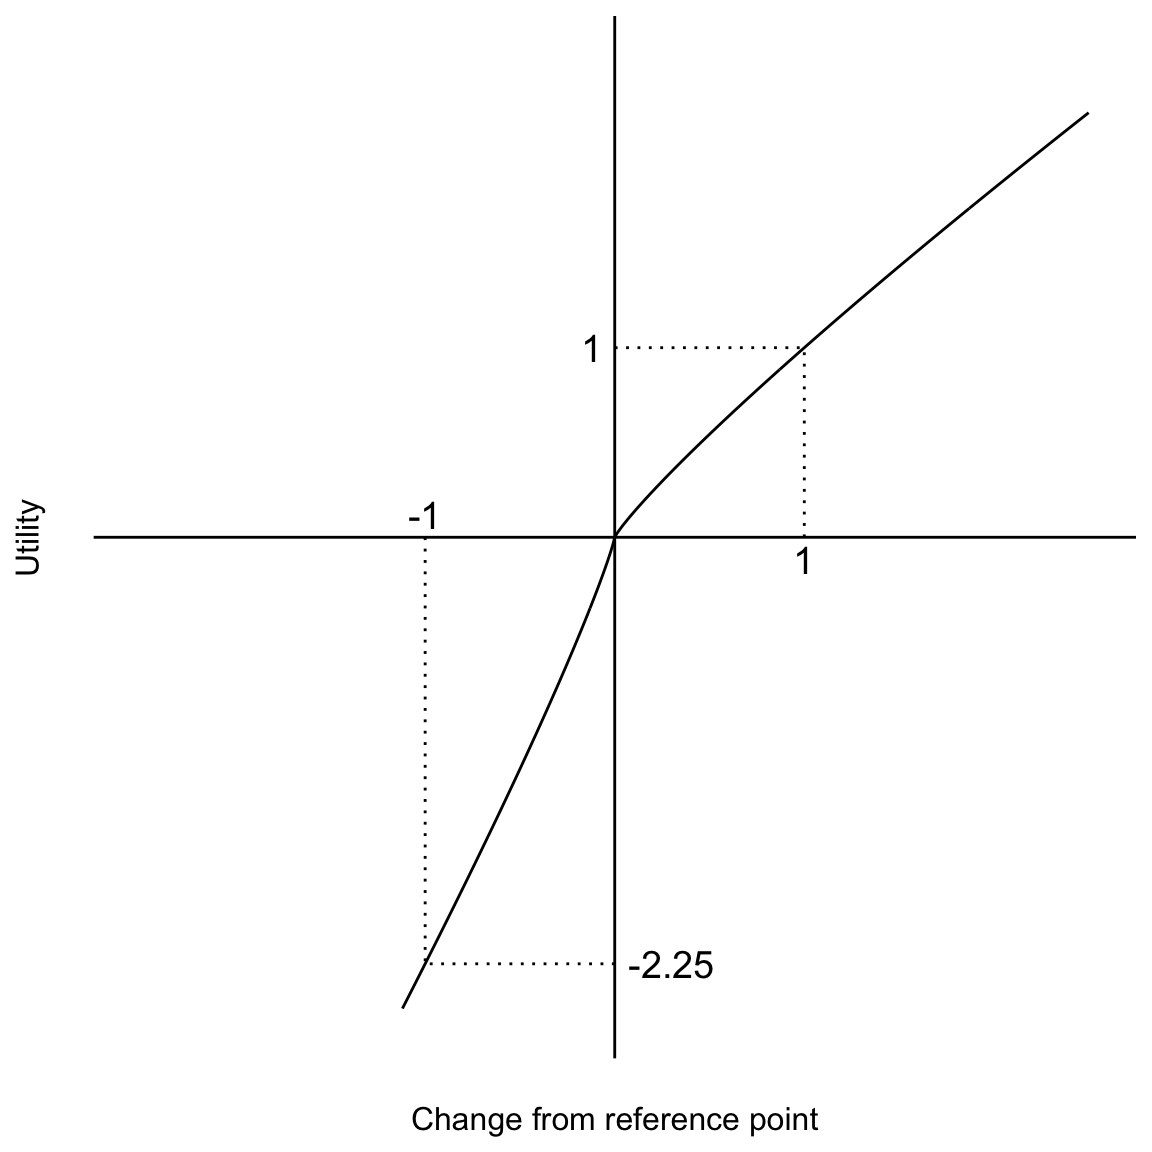
\includegraphics[width=1\linewidth]{thesis_files/figure-latex/prospect-theory-1} \caption{An example of the value function in prospect theory.}\label{fig:prospect-theory}
\end{figure}

This research is relevant to capital allocation because the project proposals
that managers evaluate invariably involve an element of risk. Therefore,
managers are likely to be affected by similar effects on risk that have been
shown in laypeople. However, hierarchical organisations offer an even more
complex situation. \textcite{lovallo2020} found that the risk profiles of lower-level
managers are lower than those of the top managers. They suggest that this may be
due to lower-level managers' loss aversion to accepting projects that may
jeopardise their job. However, the top managers recognise that a loss in one or
more business units is likely to be offset by gains in other units. Such an
inconsistency in risk profiles across the levels of an hierarchical organisation
fails to take advantage of the benefits of risk aggregation, which has long been
understood in external markets \autocite{markowitz1952}.

\textcite{lovallo2020} suggested that lower-level managers' failure to aggregate risk to
the degree desired by top executives is costing companies approximately a third
of the total EV of new project proposals. This is an example of a negative
consequence associated with ignoring statistical concepts such as risk
aggregation. It is thus critical to identify ways to support risk aggregation
across organisational hierarchies. The psychological literature shows that
people's risk aggregation is facilitated through various choice bracketing
manipulations. However, there has been no work that investigated such situations
without providing participants with feedback in between decisions; this
critically limits the external validity of this work because in the real world,
organisations evaluate several projects before seeing the outcomes of any one
decision. The experiments presented in Chapter~\ref{aggregation} investigate
the effects of choice bracketing on risk aggregation without feedback.

\subsection{Project similarity}

When evaluating project proposals, managers are likely to be influenced by the
relative similarity of the available options to each other. The extent to which
this may be true is important especially since the increase firm
diversification. Organisations are not only varied by the number of divisions
which they possess, but also by the extent of diversification. This means that
managers are likely to find themselves comparing across dissimilar types of
projects.

As mentioned above, there are likely many organisational and financial reasons
why the extent of diversification in an organisation would impact its
performance. However, the impact of psychological factors has not been
investigated. Specifically, project similarity, which is an organisational
factor, is likely to affect the project comparison process, which is a
psychological factor. This may then have downstream consequences on firm
performance through, for instance, the kinds of financial metrics that are used
and how they are evaluated. Having more similar projects to compare may mean
more attributes on which to evaluate, whereas a dissimilar comparison may lead
to a situation in which a manager has to rely on potentially unreliable metrics.

Structure-mapping theory \autocites[SMT;][]{gentner1997,gentner1983} provides a model of
comparison that psychologically distinguishes similar and dissimilar allocation
tasks. SMT models comparison as a process of bringing conceptual structures into
alignment which, when possible, puts shared dimensions into correspondence.
Alignment both highlights when two conceptual structures share dimensions, but
also highlights how the two structures differ along those shared dimensions,
called \emph{alignable differences}. For example, when comparing two oil discovery
projects, all the relevant processes of planning an exploration and measuring
the amount of hydrocarbons in a prospect might be identical, but the specific
amount measured will be different. This is the alignable difference: a
difference between the two projects that is constrained within the same
conceptual structure. However, when comparing between an oil field and a
refinery, there will be significantly more \emph{non-alignable differences}, because
the two domains do not share component dimensions. That is, many of the
processes that exist in the exploration business unit have a significantly
different dimensional structure to those in the refinery business unit, such
that it will be difficult to find meaningful alignments. More non-alignable
differences mean that there are less opportunities to make meaningful
comparisons, and so would make predicting relative project success and ranking
their priority more difficult. Chapter~\ref{alignment} experimentally
examines business project comparisons and how project alignment affects capital
allocation decisions.

When evaluating projects, managers make use of financial metrics, such as NPV.
However, such metrics are reliant on forecast estimates of, for instance, future
cash flows. Do managers take into account such inherent variance in their
decisions? This is especially important to investigate given the above
discussion. In cases of non-alignable comparison managers may rely on a
potentially unreliable metric. On the other hand, in an alignable comparison,
managers might have the option to moderate their choice based on the relative
reliability of different metrics. It is important to remember that all such
decisions are often very consequential for the manager. That is, the project
could ultimately make the company money and lead to future opportunities for the
manager, or potentially cause financial harm to the company (and subsequently
lead to a job loss). This is another example of the way in which ignoring
certain statistical concepts---here metric variance---can have negative
consequences for an organisation.

Psychological research shows that laypeople are in general quite poor at using
numerical variance information \autocite{galesic2010,konold1993,vivalt2021,batteux2020}. However, it is unclear to what extent managers would be sensitive
to variance information in the metrics associated with the projects that they
evaluate. On the one hand, perhaps managers' financial training will allow a
consideration of such variance estimates, but this might not manifest in a
situation in which managers have already been shown to be prone to biases.
Chapter~\ref{alignment} investigates whether people are as sensitive to
verbally-instructed reliability information as they are to numerical reliability
information.

\subsection{Reasoning from past cases}

Managers often use past events to reason and make predictions about the future
\autocite{einhorn1987}. Such past events may be those that happened to the individual
manager, a case from the organisation's history, or from an external source.
This will especially be the case in a project evaluation scenario when a given
project is hard to compare with the other projects at hand. However, managers
evaluating project proposals may make inappropriate comparisons when considering
the target project to other cases. For instance, when comparing a target problem
to other cases, people tend to limit the size of the comparison set to a small
number. This is often only a handful of cases, or even one. Doing this might
mean only considering potentially irrelevant surface similarity to the current
situation and not aligning the underlying causal structure. Further, this might
mean not considering other similar projects.

\textcite{tversky1974} discussed a number of biases that may influence such processes. The
availability bias is seen when people mistake the ease of retrieval of
information for its frequency. Further, research on analogical retrieval showed
that people are more likely to retrieve surface similar cases than those with a
relational connection \autocite{gentner1993}. As such, managers are likely to recall
cases that may not be sufficiently relevant to their target situation and be
overly-confident about the frequency of such cases occurring. Such a focus on a
particular case might then also lead to an anchoring effect, wherein other
decisions might be disproportionately seen as relevant. \textcite{tversky1974} also found
that people are not sensitive to properties of sample size such as the greater
amount of non-representative outcomes in small samples. This means that managers
are even less likely to appreciate the importance of considering a large sample
of cases when drawing conclusions to a target problem. \textcite{tversky1974} also note an
insensitivity to predictability, in which people do not take into account the
reliability of the information that they have to make a prediction. This might
mean that managers may struggle to ideally weigh evidence of varying degrees of
reliability.

External sources that might be used to compare to a target situation include
business case studies. Considering such examples of prior business decisions or
events are the way that most MBAs learn about the business world. Publications
such as Forbes or Harvard Business Review publicise various businesses'
successes and failures and so may create an allure to use such case studies in
the decision-making process. On the other hand, managers may have access to more
aggregated data about their industry from, for instance, consultancy companies.
How do managers use these various types of evidence in their decision-making?

Research on this topic suggests that managers tend to prefer anecdotes over
statistics, unless aided \autocite{wainberg2018}. This is a concern because \textcite{gavetti2005}
suggests that managers often make use of case studies quite poorly. The analogy
literature draws a distinction between surface similarity, in which a mapping is
made between easily identifiable but potentially functionally irrelevant
attributes, and relational similarity, in which the underlying mechanism is
considered. Are managers sensitive to the deeper causal mechanisms that underlie
the anecdotes they judge? Or are they simply influenced by surface similarity?
Chapter~\ref{anecdotes} investigates the extent to which people moderate their
reliance on anecdotes or aggregated data by the relevance of the anecdote to the
target project during capital allocation. It also considers whether people are
sensitive to information about the distribution from which the anecdote was
sampled. Ignoring this statistical concept can have negative consequences for an
organisation by potentially over- or under-estimating the relevance of a past
case and therefore making an ill-informed investment.

\hypertarget{chapter-overview}{%
\section{Chapter overview}\label{chapter-overview}}

In sum, the potential consequences of a diversified hierarchical structure are
that business projects will be considered one at a time, and if they are
considered together, disparate project types will make comparisons hard.
Considering projects one by one might mean that risk is not aggregated across
projects and therefore value is lost. The difficultly to compare will lead to
both potentially relying on unreliable metrics, and relying on improper
anecdotal evidence. The thesis is that people often go half-way. They do not
completely disregard the normative strategy, but also struggle to moderate their
decisions when it comes to statistical concepts such as aggregation, variance,
and sampling.

The previous section identified three capital allocation processes that are
currently under-studied and so are important to investigate further. First, the
evaluation of individual project proposals might lead to managers only
considering such projects one at a time, despite the opportunity of aggregating
a portfolio of such projects. The choice bracketing literature suggests that
there are ways of facilitating such aggregation, but does not investigate this
without providing participants inter-trial feedback. Second, in situations in
which managers compare multiple projects, the structural alignment literature
suggests that managers in diversified firms will struggle to allocate capital,
more than those in more integrated firms. Further, these managers might not be
sensitive to the variance inherent in the financial metrics they rely on. Third,
a difficulty to compare across existing projects might instead mean a reliance
on prior case studies from personal or external experience. Research on
anecdotal bias suggests that managers might rely more on such case studies than
on aggregated data, but it is unclear whether they will use anecdote relevance
to moderate their decisions. Further, it is unclear if they will appropriately
use information about the anecdote's sample distribution.

The rest of this thesis investigates the psychology of capital allocation
decisions in three chapters that describe empirical work, two theoretical
chapters, and a general discussion chapter. Chapter~\ref{aggregation} describes
two experiments that investigate the effects of choice bracketing on risk
aggregation without feedback. Chapter~\ref{interstitial-1} is a short
theoretical chapter that discusses the difference between evaluating project
proposals with inherent budget estimates and the process of allocating an
existing budget top-down. Chapter~\ref{alignment} describes three experiments
that investigate the effects of alignment and reliability type---verbal or
numerical---on allocations. Chapter~\ref{interstitial-2} is another short
theoretical chapter that discusses the trade-offs that people make when using
information to evaluate project proposal options. Chapter~\ref{anecdotes}
describes two experiments that investigate the effects of anecdote similarity on
the anecdotal bias. Finally, Chapter~\ref{discussion} discusses the theoretical
and practical implications of the empirical chapters and concludes the thesis.

\newpage

\printbibliography[segment=\therefsegment,heading=subbibintoc]



\begin{savequote}
Cultivate the habit of surveying and testing a prospective action before
undertaking it. Before you proceed, step back and look at the big
picture, lest you act rashly on raw impulse.
\qauthor{---\textcite{epictetus1995}}\end{savequote}

\hypertarget{aggregation}{%
\chapter{Effect of choice bracketing on risk aggregation in repeated-play gambles with no feedback}\label{aggregation}}

\chaptermark{Effect of choice bracketing on risk aggregation}

\minitoc

\section{Introduction}

Investors know not to put all their eggs in one basket. Ever since work on
modern portfolio theory \autocite{markowitz1952}, it has been clear that combining the
risk of a set of individual investments reduces the overall risk of the
portfolio of investments. But what about situations in which it is not clear
that a set of investments fit together as a portfolio? Personal decisions such
as buying a car or moving cities are typically evaluated independently, as are
business decisions such as a farm investing in new cropping technology or a
multi-business firm building a mine.

While these decisions are separated in time, they are often not so far apart
that it is easy to learn from past outcomes (and sometimes the outcomes
themselves are unclear). This is because the outcomes of large investments are
often delayed. As such, the decision-maker cannot always use the knowledge of
the returns of one investment when evaluating a subsequent investment. Any
results that a farmer may identify from using a new technology will only become
apparent after many seasons of use. Similarly, it will take many years for a
multi-business firm to begin to estimate whether the output of a mine resulted
in the expected return on investment. These are the decisions that this chapter
investigates: sequences of large risky choices without immediate outcomes.

Risk aggregation is the combination of probability or variance information (or
both) associated with certain outcomes for the purpose of understanding that
information more comprehensively \autocite{bjornsen2019}. However, the psychological
literature suggests that this process may be difficult for people to use. Work
on prospect theory \autocite{kahneman1979} suggests that people's evaluation of gambles
does not conform to expected utility theory and is prone to framing effects.
Specifically, people typically evaluate gambles one by one \autocite{rabin2009,tversky1981,kahneman1993}. As such, it is unlikely that people will be able
to aggregate risk when they do not perceive a series of investments as a
portfolio. So, what would encourage people to aggregate risk? The literature on
\emph{choice bracketing} \autocite{read1999} shows that grouping a set of individual gambles
together facilitates risk aggregation. As such, the current work provides two
primary contributions. First, this work is the first to investigate the effect
of choice bracketing on risk aggregation in independent gambles evaluated
without immediate returns. Second, this work introduces novel choice bracketing
manipulations.

The earlier work on risk aggregation essentially did the aggregating work for
the participants. For example, experimenters provided participants with an
outcome probability distribution, usually with an explicit indication to group
the choices together, such as by asking for a single decision to be made on a
set of identical gambles. Other work addressed the more realistic situation of a
set of independent gambles. However, most of this work provided participants
with the outcomes of their choices before the subsequent choice. In these
paradigms participants experienced individual outcomes from the eventual outcome
distribution of the gambles, meaning that aggregation was confounded with
learning.

As mentioned above, in real-life there is usually a significant delay between
the choice a person or firm makes and the outcome of that choice, and there are
likely to be several interim choices in the meantime. This is especially true
for business executives, who would typically have to wait months or years before
beginning to understand the consequences of their decision, and even then the
outcome may be unclear. However, previous work did not investigate the effect of
choice bracketing on risky choice without feedback. This is surprising, since
choice bracketing is exactly the kind of process that should promote aggregation
in these more realistic decisions. As such, this chapter investigated new ways
of encouraging participants to bracket their risky choices, but with a paradigm
that involves a series of independent choices without feedback. In this way, the
paradigm is more isometric with real-life risky choice.

\subsection{Multi-play gambles}

Despite the difficulties of risk aggregation, people seem to aggregate ``naively''
when considering multiple gambles. \textcite{samuelson1963} told of a colleague who
rejected a gamble that involved a 50\% chance of gaining \$200 and a 50\% of losing
\$100, despite the gamble's positive Expected Value (EV). That is, \(200 \cdot 0.5 - 100 \cdot 0.5 = 50\). Rejection of a positive EV gamble out of fear of the
possible loss is classic loss aversion. However, the same colleague said he
would accept 100 plays of the same gamble. Samuelson argued that this choice is
irrational.\footnote{Other work suggests that it is consistent with expected utility
  theory, once certain assumptions are added \autocites[e.g.,][]{ross1999,aloysius2007}.
  However, a normative discussion is out of the scope of the present work.} Intuitively, it is clear that over the course of 100
gambles, the positive EV wins out, and a net loss of money is extremely
unlikely. Samuelson's colleague was more risk averse when making a single
decision about one gamble (a \emph{single-play} gamble), than when making a single
decision about multiple (in this case 100) identical gambles (a \emph{multi-play}
gamble).\footnote{This chapter uses the terminology for gamble types used in
  \textcite{bristow2011}, and \textcite{camilleri2013}.}

\textcite{wedell1994} replicated the \textcite{samuelson1963} anecdote experimentally with a gamble
involving a potential gain of \$100 and a potential loss of \$50. Participants
accepted the multi-play gamble of 100 plays more than the single-play gamble.
This effect has since been replicated with different outcomes and probabilities,
both with hypothetical and real money. Some participants often require fewer
than 10 plays of a previously rejected gamble in order to accept it \autocite{dekay2005,keren1991,montgomery1982,redelmeier1992}. Other similar studies found a
multi-play effect that was in the predicted direction but not significant
\autocite{barron2003,benartzi1999,klos2005,langer2001}. Further, the effect is not
seen when participants do not perceive gamble outcomes as fungible \autocite{dekay2006,dekay2005,dekay2011} or when choice is continuous rather than discrete
\autocite{bristow2011}.

However, multi-play effects are likely robust, since there is also evidence that
such gambles reduce a variety of cognitive biases. These include common-ratio
effects \autocite{keren1987,keren1991,dekay2006}, preference reversals
\autocite{wedell1990}, ambiguity aversion \autocite{liu2009}, and the illusion of control
\autocite{koehler1994}. Participants are also more likely to use explicitly provided EVs
in multi-play gambles \autocite{li2003}, show eye movements more congruent with an EV
model than single-play gambles \autocite{su2013}, and judge multi-play gambles as
riskier \autocite{joag1990}.

People prefer multi-play gambles that are displayed with an aggregated outcome
distribution of those gambles than those without \autocite{benartzi1999,redelmeier1992,klos2013,webb2017,coombs1971,venkatraman2006,dekay2005,langer2001,keren1991}. This is because these distributions
present the probabilities of all the different possible outcomes, so very
clearly show the rarity of a loss. Note that this does not seems to hold when
returns are calculated as percentages, rather than fixed dollar amounts
\autocite{stutzer2013}; and when participants do not perceive gamble outcomes as
fungible \autocite{dekay2005}. However, when this effect is demonstrated, the multi-play
gamble is usually set up such that its (binomial) outcome distribution shows a
relatively low chance of losing any money and a very low chance of losing a lot
of money. For instance, Figure~\ref{fig:samuelson-distribution-10} shows the
outcome distribution of the \textcite{samuelson1963} gamble played 10 times. Outcome
distributions of this sort do the aggregating work for the participants, making
the attractiveness of the multi-play gamble clearer. This work suggests that
participants can comprehend and respond to aggregated risk, but that they
struggle to compute the aggregation without external help.



\begin{figure}
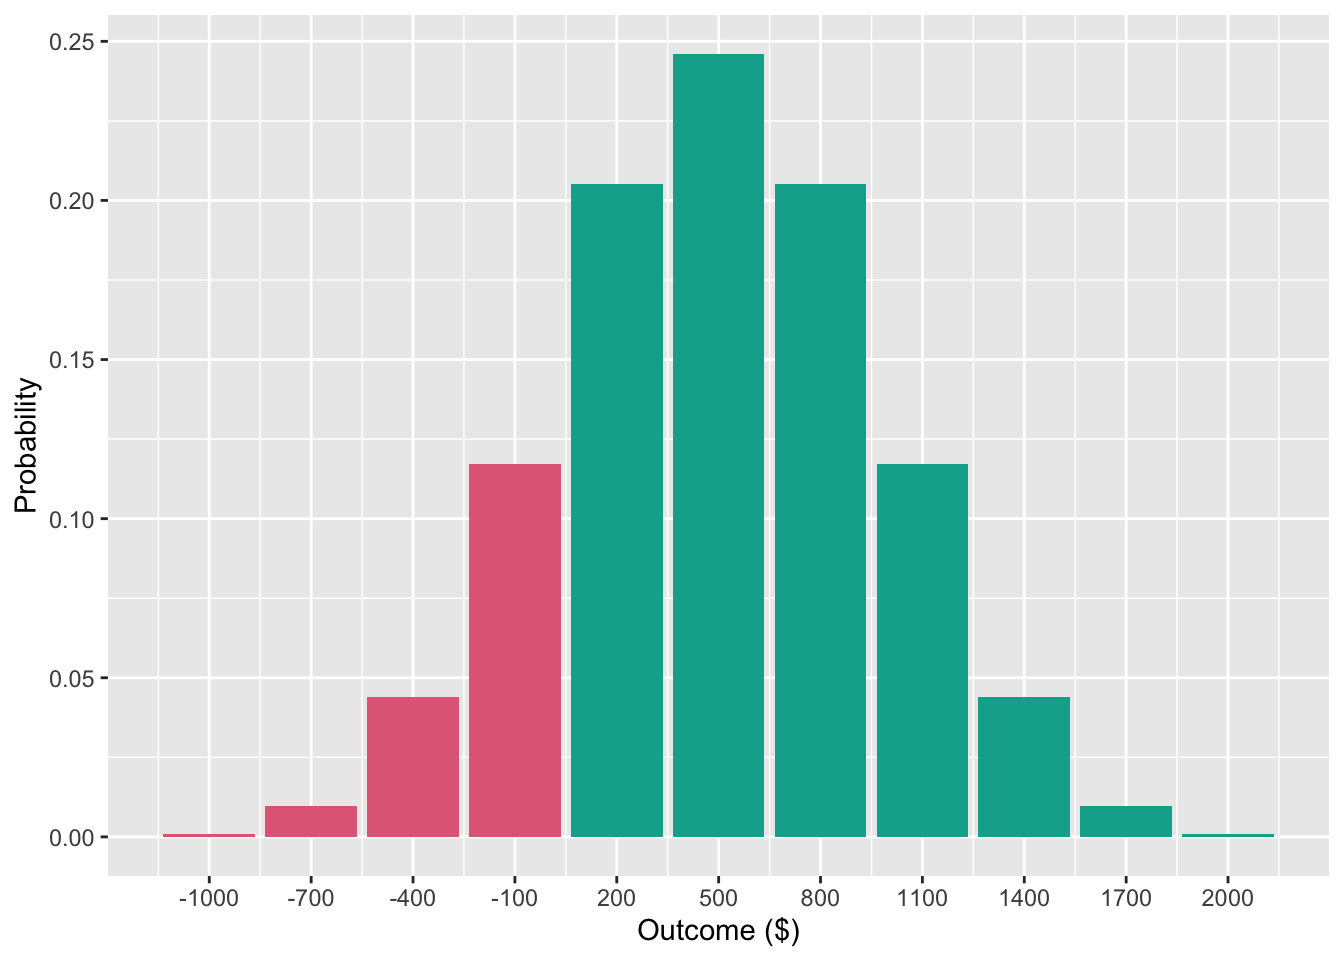
\includegraphics[width=1\linewidth]{thesis_files/figure-latex/samuelson-distribution-10-1} \caption{The outcome probability distribution of the \textcite{samuelson1963} gamble (50\% chance of gaining \$200 and a 50\% of losing \$100) played 10 times.}\label{fig:samuelson-distribution-10}
\end{figure}

\subsection{Repeated-play gambles}

Decisions in real life are usually sequential, and rarely identical as in the
multi-play paradigm \autocite[cf.][]{barron2003}. That is, people tend to be confronted
with individual choices whose outcomes and outcome probabilities are different
from one choice to another, and these choices occur at different points in time.
In a business setting this can be seen in decisions about whether to invest in
new projects; proposals and opportunities differ widely and occur at different
times. Managers are not ever simply asked: ``here are 10 identical investments to
consider; do you want all or none of them?''

In \emph{repeated-play} (rather than multi-play) gamble paradigms, participants make
decisions about a series of individual gambles. Research using this paradigm
found that people are less risk averse both when outcomes for a series of
gambles are evaluated less frequently and the subsequent decisions are made less
frequently \autocite{gneezy1997,thaler1997,bellemare2005,beshears2016}. People are
also less risk averse (for positive EV gambles) when they receive feedback after
each decision or are able to sample from the distribution of possible outcomes
before making a choice \autocite{camilleri2011,camilleri2013,barron2003,wulff2018,ludvig2011,hertwig2004,jessup2008}. Other work found that loss aversion is
mitigated when people are explicitly instructed to consider the options as a
part of a portfolio \autocite{sokolhessner2009,sokolhessner2012}.

These studies are closer to real-life decisions than the multi-play gamble
paradigm, because they involve a set of separate gamble decisions, rather than a
single decision about a set of gambles. However, for the most part, the
experiments used in the repeated-play gamble literature use various forms of
feedback throughout the course of the experiment. That is, participants are
shown the outcomes of their gambles before they make more decisions. This
paradigm is known as \emph{experience-based choice}. In \emph{description-based choice},
on the other hand, the gamble is simply presented to the participant without any
feedback, as in the multi-play gambles above. In real life, people rarely see
the immediate outcomes of their risky choices, and even less so in business
settings, where any return on investment often takes years to manifest.

Only a limited number of studies have used a repeated-play paradigm without
feedback. For instance, \textcite{jessup2008} and \textcite{hertwig2004} investigated the effects of
feedback in repeated-play gambles on the weighting of small probabilities, and
had a no-feedback control condition. Other work similarly used individual
description-based gambles presented sequentially \autocites[e.g.,][]{ert2013,joag1990}.
However, these studies did not attempt to facilitate participants' risk
aggregation. \textcite{haisley2008} provided limited evidence for facilitating risk
aggregation. They gave participants the opportunity to buy five (negative EV)
lottery tickets, and either presented them one at a time, or together.
Participants bought fewer tickets, when they considered them jointly, thereby
maximising EV. However, the experimenters did not specify the outcomes and
probabilities of each gamble, meaning that it is unclear if participants
understood the independent lotteries as identical or non-identical. This reduces
the external validity of the study, as most independent risky choice involves
non-identical outcomes and probabilities. In sum, these studies were not
designed to research how to facilitate risk aggregation and reduce loss
aversion. This chapter is novel because its goal is to facilitate risk
aggregation without the experimental artefact of immediate feedback.

\subsection{Choice bracketing}

Research in psychology and economics has identified ways of facilitating risk
aggregation by encouraging people to group their choices. Specifically, people
aggregate more when they consider the consequences of their choices together
(broad bracketing) than when they consider them individually \autocite[narrow
bracketing;][]{read1999}. In multi-play gambles (especially when displayed with
an outcome distribution), choices are inherently bracketed broadly because a
single choice is made about multiple gambles. Similarly, studies that used
repeated-play gambles facilitated risk-tolerance through what can in hindsight
be considered broad bracketing. For instance, when \textcite{thaler1997} presented gamble
outcomes less frequently, they allowed participants to consider longer time
increments with a single evaluation.

Both the original \textcite{samuelson1963} anecdote and its subsequent replications show
that people do have an intuition for aggregation even without the risk being
calculated exactly for them. This chapter tests whether that same intuition can
be elicited and applied across sets of unique bets. What are the minimal
conditions required to encourage aggregation? The multi-play gamble work
suggests that participants can engage in a more intuitive form of aggregation
when provided with the right contextual cues. Investigating the effects of more
subtle cues will help shed light on the cognitive processes underlying choice
bracketing. Of course, the effects of more subtle cues would not eliminate the
utility of explicit financial education, but they will help the design of
decision-making contexts to best align with such instruction.

One way of potentially facilitating risk aggregation is to highlight to
participants the number of total options that are available to them.
\textcite{sokolhessner2009} and \textcite{sokolhessner2012} reduced risk aversion using lengthy
instructions that encouraged participants to ``think like a trader.'' This meant
considering all the repeated-play gambles as a portfolio, as opposed to
considering them individually. However, this was quite a strong manipulation
that is perhaps unrealistic in real world. A more subtle cue could involve
simply making participants aware that they are going to be making a series of
choices. If people possess an intuitive understanding of aggregation, as
suggested above, then this kind of contextual cue will also facilitate
aggregation.

In addition to simply informing participants that they will make a series of
choices, making the choices more readily comparable may facilitate broad
bracketing, and thus risk aggregation. Consider the inverse situation wherein a
lack of comparability between choices may prevent broad bracketing, such as when
an executive for a multi-business firm makes decisions across multiple distinct
industries. Of course, the similarity of decision contexts does not change the
maths of risk aggregation, but may well affect whether people do aggregate risk
across decisions. \textcite{dekay2005} found that multi-play effects are not seen when
choices are not considered fungible. For instance, participants aggregated
across dollar amounts, but not across patients in a medical decision. As such,
people may behave similarly when considering a set of dissimilar choices if they
do not consider them fungible.

There is further suggestive evidence that the similarity of a set of choices to
one another will affect choice bracketing. Choices whose differences are easy to
compare (alignable differences) are weighted heavier than those that are
difficult to compare \autocite{markman1995,markman2010}. Increased similarity across a
set of choices may both highlight the ability for those choices to be bracketed,
and further facilitate risk aggregation through the comparable attributes.
However, it is possible that increased similarity will facilitate risk
aggregation even without a tangible benefit to the underlying calculations. That
is, it is possible that simply manipulating the similarity of
financially-irrelevant semantics of a choice set will make people less risk
averse. If so, then this will be by virtue of an implicit risk aggregation in
which the mere awareness of the possibility of a grouping of choices reduces
risk aversion. It is important to investigate the effect of similarity
especially because in managerial settings, executives in multi-business firms
will often have to make comparisons across industries that are hard to compare.
For instance, General Electric currently develops both analytic software
products and jet engines for the military. They had been even more diversified
previously, at one stage simultaneously developing home appliances and owning
the NBC television network.

In addition to the similarity between choices, how choices are presented may
affect how easily they are compared, and thus whether or not the multiple
subsequent effects listed above would come to fruition. As mentioned above,
\textcite{haisley2008} found a higher degree of EV maximisation when gambles were
presented jointly, rather than separately. Similarly, \textcite{hsee1999} found that
people's choices were affected by whether they viewed the attributes of the
choices separately or jointly. Their \emph{evaluability hypothesis} suggests that
attributes that are difficult to evaluate will have a greater impact on joint
presentation than separate presentation. Joint presentation is a form of broad
bracketing because it forces a participant to view of all the components of a
decision together. Participants may therefore be more likely to consider
aggregating the risk involved in a set of choices when all those choices are in
view. Joint presentation potentially reduces the working memory load otherwise
needed to maintain that set of choices. As such, it is quite possible that a
combination of highly similar choices, presented jointly will lead to the
highest likelihood of broad bracketing, and thus risk aggregation.

\textcite{moher2010} replicated \textcite{gneezy1997}, but separately manipulated the number of
gambles seen per trial and feedback frequency. They found that participants were
less risk averse when viewing a set of three gambles per trial, than when
viewing only one. However, they only found this effect with a set of identical
outcomes. When outcomes were non-identical, there was no effect of presentation.
However, participants were always presented with gamble outcomes for each trial,
so it is unclear to what extent this influenced participants' ability to bracket
broadly. In fact, when seeing gambles separately, participants were less risk
averse when receiving feedback for each trial, compared to every three trials.
Testing a presentation manipulation without the confound of feedback will help
to clarify this effect.

\subsection{Internal capital market investment context}

Executives of large, successful firms are often viewed as fearless risk-takers
who take on risky projects to generate innovation and growth. However, the
available evidence suggests that executives do not view themselves that way
\autocite{swalm1966,march1987}. Executives typically evaluate multiple investments
over time. Risk aggregation is sensible when investments are only partially
correlated (i.e., the success of one does not influence the success of another).
It is sensible to take on a set of risky investments with positive EV, where
each investment has some chance of loss, because those that succeed will make up
for those that failed. These benefits are well-known in stock market investment
settings, thanks to Nobel laureate Harry Markowitz's work on modern portfolio
theory \autocite*{markowitz1952}.

However, it is unclear whether the general public and even business managers use
this concept, due to the extent of risk aversion in both those populations
\autocites[e.g.,][]{tversky1992,march1987}. In fact, executives treat risk like the rest
of us; they view investments one at a time, are risk averse in the domain of
gains, and are risk seeking in the domain of losses \autocite{maccrimmon1986,swalm1966,lovallo2020}. However, it is understandable why risk aggregation is
foreign to most people; outside of an investment portfolio selection situation,
it is unlikely for people to spontaneously group a selection of individual risky
choices. Usually in life, people encounter risky choices sequentially, and so
the risk of each individual choice is more salient than the aggregated risk of
an arbitrary combination of choices.

\textcite{lovallo2020} show that executives treat investments within their own company in
isolation. In multi-business firms, the managers of each business unit often
make the investment decisions about individual projects. As such, they often do
not consider the scope of their decisions in the context of the entire company.
For instance, Nobel laureate Richard Thaler offered 25 division managers working
for the same firm a hypothetical investment that involves a 50\% chance of
gaining \$2 million for the company and a 50\% chance of losing \$1 million
\autocite*{thaler1999}. Only three managers said they would accept the investment.
However, the CEO indicated that he would have clearly preferred managers to
accept all the investments. To each middle-manager, the choice represents a risk
of loss for their division and potentially their job, whereas for the CEO the
entire portfolio of choices represents a worthwhile risk.

This chapter investigates risky choice in the context of business project
investment internal to a company because this is a real-world context where
choice bracketing is important and currently under-appreciated \autocite{lovallo2020}.
The participants in these experiments were taken from a population that does not
have extensive managerial experience. However, in such a population a lack of
risk aggregation is most likely more common, and the variables used here are
readily applicable to the financial decisions that laypeople make. For instance,
one of the real-world applications of the choice bracketing literature has been
to use outcome distributions and increased time horizons to encourage investment
in high risk, but high EV, retirement funds \autocite[e.g.,][]{benartzi1999}. Otherwise,
people typically prefer low risk, low EV, funds. Further, using laypeople
eliminates potential differences in prior experience with the management-based
decision-context. Upcoming research will focus on managers with context-specific
experience to investigate the effects of that experience.

\hypertarget{aggregation-1}{%
\section{Experiment~1}\label{aggregation-1}}

Experiment~1 investigated the effect of three choice bracketing manipulations on
risky choice in hypothetical capital allocation scenarios. Previous research
had low ecological validity because of the use of multi-play paradigms or
feedback. In this experiment, the risky choice task was a description-based
repeated-play paradigm. This means that participants had to make a choice about
whether to accept a number of different hypothetical investments, but were not
provided with the outcome of their choices after each decision. The variables of
interest were the similarity of the choices, whether the choices were presented
together or separately, and whether participants were aware of the number of
choices that they would be making.

The values and probabilities of the gambles were set up such that each
individual gamble, as well as the aggregation of all the gambles, would be
attractive to a rational agent interested in maximising EV. As such, the key
dependent measure was the proportion of risky choices participants accepted.

Previous research suggests that people will be willing to make more risky
choices when explicitly told to bracket their choices \autocite{sokolhessner2009,sokolhessner2012}. Therefore, Experiment~1 tested the following:

\begin{hypothesis}[Awareness main effect]
\protect\hypertarget{hyp:awareness-aggregation-1}{}{\label{hyp:awareness-aggregation-1} \iffalse (Awareness main effect) \fi{} }Participants that know how many projects to expect will make more risky choices
than participants that are unaware.
\end{hypothesis}

Further, previous work suggests that joint presentation is a form of broad
bracketing \autocites[e.g.,][]{moher2010,hsee1999}. Therefore, Experiment~1 tested the
following:

\begin{hypothesis}[Presentation main effect]
\protect\hypertarget{hyp:presentation-aggregation-1}{}{\label{hyp:presentation-aggregation-1} \iffalse (Presentation main effect) \fi{} }Participants will make more risky choices when seeing projects jointly than when
seeing them separately.
\end{hypothesis}

Similarity of options has also been shown to affect the way people bracket their
choices \autocite[e.g.,][]{dekay2005}. Therefore, Experiment~1 tested the following:

\begin{hypothesis}[Similarity main effect]
\protect\hypertarget{hyp:similarity-aggregation-1}{}{\label{hyp:similarity-aggregation-1} \iffalse (Similarity main effect) \fi{} }Participants that see projects from the same industry will make more risky
choices than participants that see projects from different industries.
\end{hypothesis}

\subsection{Method}

\subsubsection{Participants}

One hundred and ninety-eight people (82 female) were recruited from the online recruitment platform Prolific. Participants were compensated at a rate of £5 an hour. The average age was 32.52 (\emph{SD} = 11.42, \emph{min} = 18, \emph{max} = 69). Participants reported an average of 7.01 (\emph{SD} = 9.1, \emph{min} = 0, \emph{max} = 42) years of work in a business setting, and an average of 1.7 (\emph{SD} = 2.85, \emph{min} = 0, \emph{max} = 20) years of business education. The mean completion time was 12.04 (\emph{SD} = 11.29, \emph{min} = 3.1, \emph{max} = 112.4) minutes.~Table~\ref{tab:condition-allocation-aggregation-1}
shows the between-subjects condition allocation.

\begin{table}[tbp]

\begin{center}
\begin{threeparttable}

\caption{\label{tab:condition-allocation-aggregation-1}Experiment 1 group allocation.}

\begin{tabular}{lll}
\toprule
Similarity & \multicolumn{1}{c}{Awareness} & \multicolumn{1}{c}{N}\\
\midrule
High & Aware & 53\\
High & Naive & 53\\
Low & Aware & 47\\
Low & Naive & 45\\
Total & - & 198\\
\bottomrule
\end{tabular}

\end{threeparttable}
\end{center}

\end{table}

\subsubsection{Materials}

\hypertarget{instructions-materials-aggregation-1}{%
\paragraph{Instructions}\label{instructions-materials-aggregation-1}}

Participants were told to imagine that they are executives in a large company
and that they will need to decide about investing in a number of hypothetical
business projects. The appendix shows these instructions in
Figure~\ref{fig:instructions-materials-aggregation-1}.

\hypertarget{task-aggregation-1}{%
\paragraph{Risky investment task}\label{task-aggregation-1}}

Participants saw 10 short descriptions of business projects, and were asked
whether they would invest in that project or not. Each description included the
name of the hypothetical business, the amount they forecast the project to cost,
the amount the project is forecast to make, and probabilities for these
forecasts. The project values were selected so that the projects appeared
attractive when aggregated, and unattractive when segregated \autocite[see][]{langer2001}.
These values were different for each project, but followed a set of constraints
for each project's EV and the probability of any loss given the outcome
distribution of all 10 projects (\(P(\text{loss}_{aggregated})\)). Further, there
was a constraint on the gambles' loss aversion coefficient (\(\lambda\)), which is
a measure of people's greater sensitivity to losses compared to gains. The
constraints were:

\begin{enumerate}
\def\labelenumi{\arabic{enumi}.}
\item
  \(\text{EV} > 0\);
\item
  \(\lambda < 2.25\); and
\item
  \(P(\text{loss}_{aggregated}) < 0.1\).
\end{enumerate}

As such, each project cannot be considered to be a loss in terms of expected
value, but also would not be an easy choice for investment, because of the low
\(\lambda\) \autocite[made to be lower than the median loss aversion coefficient calculated
in][]{tversky1992}. Further, since people are especially sensitive to loss
probabilities \autocite{zeisberger2020,kahneman1979}, an arbitrarily low
\(P(\text{loss}_{aggregated})\) was chosen to make investment in the complete set
of projects seem attractive. The actual probability of a loss given the outcome
distribution used in the experiment was 0.09.
This was calculated by summing all probabilities in the Poisson binomial
distribution whose outcomes were less than zero. For comparison,
\(P(\text{loss}_{aggregated})\) = 0.17
for 10 plays of the \textcite{samuelson1963} gamble. The highest probability of a loss for
any single gamble (\(P(\text{loss}_{single})\)) was
0.80.
Figure~\ref{fig:project-choice-aggregation-1} shows an example of a description
of a project in this task.



\begin{figure}
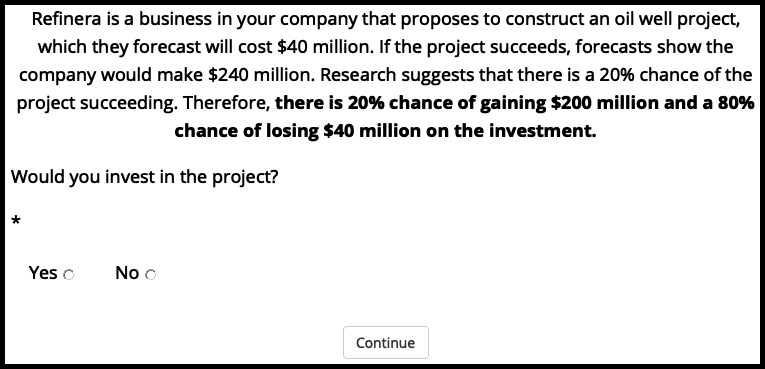
\includegraphics[width=1\linewidth]{thesis_files/figure-latex/project-choice-aggregation-1-1} \caption{Example of a project choice display in Experiment~1. Border added for clarity.}\label{fig:project-choice-aggregation-1}
\end{figure}

In the high similarity condition, these project descriptions were all about one
type of project (in this case an oil well project) and were all from the same
business. In the low similarity condition, each project was from a different
industry. In the joint presentation condition, the 10 projects were all
displayed on the one webpage, whereas in the separate presentation condition
each was displayed on a different webpage. Participants in the aware condition
saw the display shown in Figure~\ref{fig:awareness-aware-aggregation-1} before
their separate presentation display. Those in the naive condition simply
proceeded without this message. The financial and probability values were
identical regardless of condition, and the order of each set of 10 projects was
randomised.



\begin{figure}

\includegraphics[width=1\linewidth]{thesis_files/figure-latex/awareness-aware-aggregation-1-1} \caption{The display seen by those in the aware condition of Experiment~1. Border added for clarity.}\label{fig:awareness-aware-aggregation-1}
\end{figure}

Although the project descriptions were succinct, and the decisions in the task
were made quickly, they reflect real decisions in businesses in critical ways.
Companies that consider their forecast estimates probabilistically (i.e., do not
simply use the most likely estimate as the only estimate) do frame their options
as likelihoods of certain monetary outcomes.

\hypertarget{outcome-distribution-materials-aggregation-1}{%
\paragraph{Outcome distribution decision}\label{outcome-distribution-materials-aggregation-1}}

Participants were asked if they would invest in the last 10 projects they saw
and were provided with a graph of the outcome probability distribution of the 10
projects. The appendix shows this graph in
Figure~\ref{fig:project-choice-aggregated-aggregation-1}. A coding error was
discovered after collecting data. This was an error in the generation of
gambles, which meant that the outcome distribution decision data could not be
used. Therefore, the effect of outcome distribution will not be discussed until
Experiment~2, which fixed this issue.
Appendix~\ref{outcome-distribution-aggregation-1} presents an analysis of this
data, and describes the coding error and its implications.

\paragraph{Follow-up gambles}

Participants were shown four further sets of gambles (11 total) that functioned
to check participant attention and replicate the gambles from \textcite{samuelson1963} and
\textcite{redelmeier1992}. See Appendix~\ref{follow-up-materials-aggregation-1-appendix}
for details.

\subsubsection{Procedure}

Participants read the instructions and completed the risky investment task,
first in the separate presentation condition, and then in the joint condition.
They then made the outcome distribution decision and responded to the 11
follow-up gambles.

\hypertarget{results-aggregation-1}{%
\subsection{Results}\label{results-aggregation-1}}

\subsubsection{Project choice}

A three-way ANOVA was conducted to investigate the effects of similarity,
awareness, and presentation on the proportion of participants' decision to
invest in the 10 projects. As seen in
Figure~\ref{fig:plot-aggregation-1-awareness}, participants invested more when
they were told that there will be 10 projects, compared to when they were not
told this, \(F(1, 194) = 9.52\), \(p = .002\), \(\hat{\eta}^2_p = .047\). As seen in
Figure~\ref{fig:plot-aggregation-1-presentation}, participants invested more
when viewing the projects jointly, compared to when they viewed them separately,
\(F(1, 194) = 28.14\), \(p < .001\), \(\hat{\eta}^2_p = .127\). Although there was no main effect of
similarity, \(F(1, 194) = 1.63\), \(p = .204\), \(\hat{\eta}^2_p = .008\), the interaction between
similarity and presentation was significant,
\(F(1, 194) = 4.31\), \(p = .039\), \(\hat{\eta}^2_p = .022\) (see
Figure~\ref{fig:plot-aggregation-1-similarity-presentation}). Specifically, the
presentation effect was stronger in the high similarity condition,
\(\Delta M = 0.07\), 95\% CI \([0.04,~0.09]\), \(t(194) = 5.29\), \(p < .001\), than in the low similarity
condition, \(\Delta M = 0.03\), 95\% CI \([0.00,~0.05]\), \(t(194) = 2.06\), \(p = .041\). These findings
suggest that it is possible to facilitate risk aggregation with subtle choice
bracketing manipulations.



\begin{figure}
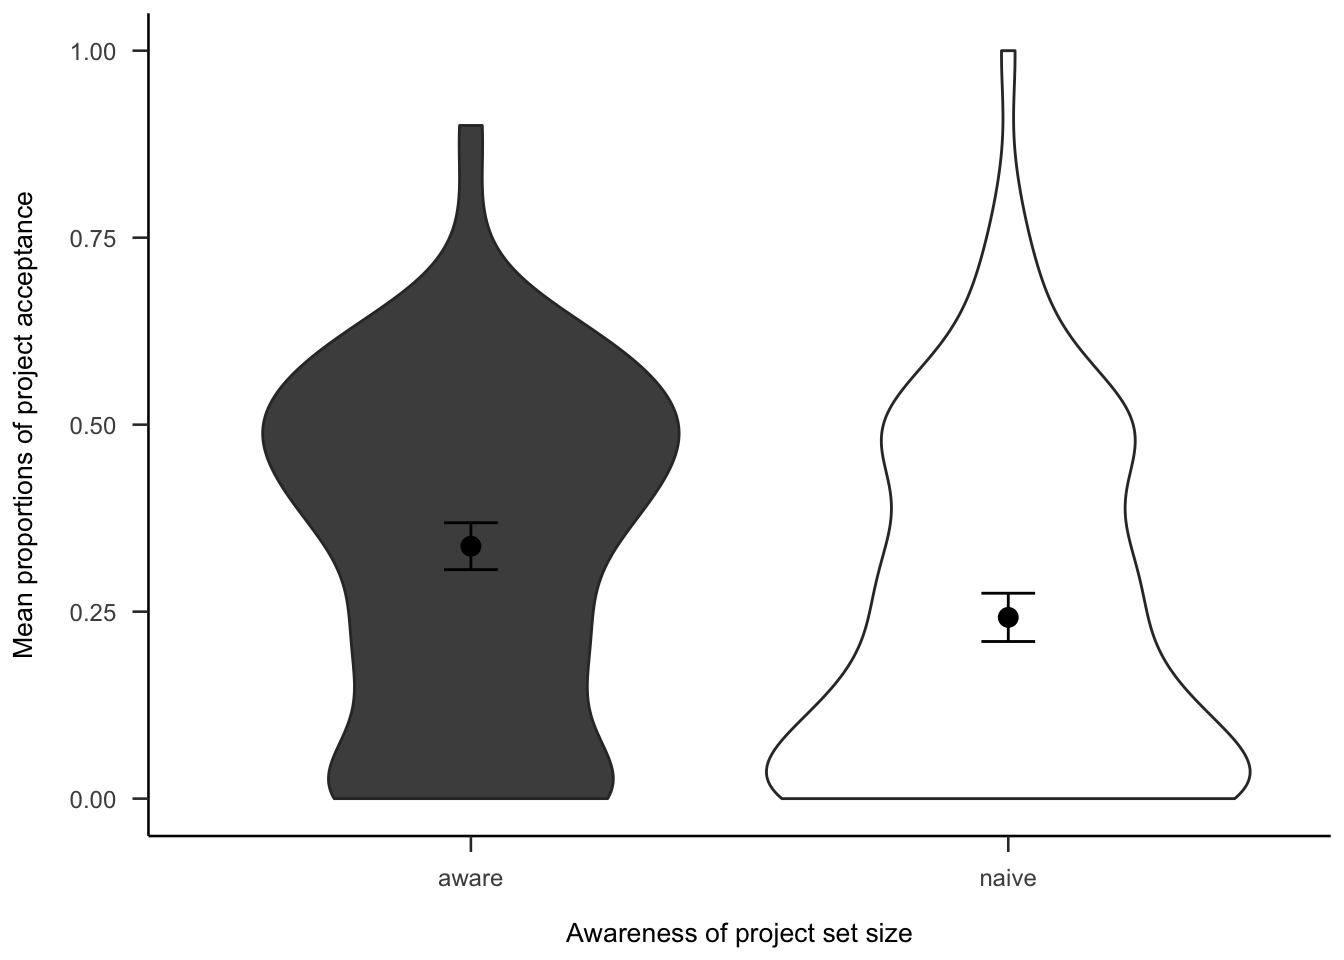
\includegraphics[width=1\linewidth]{thesis_files/figure-latex/plot-aggregation-1-awareness-1} \caption{Mean proportions of decisions to invest in each set of 10 projects, by awareness conditions. Error bars represent 95\% confidence intervals.}\label{fig:plot-aggregation-1-awareness}
\end{figure}



\begin{figure}
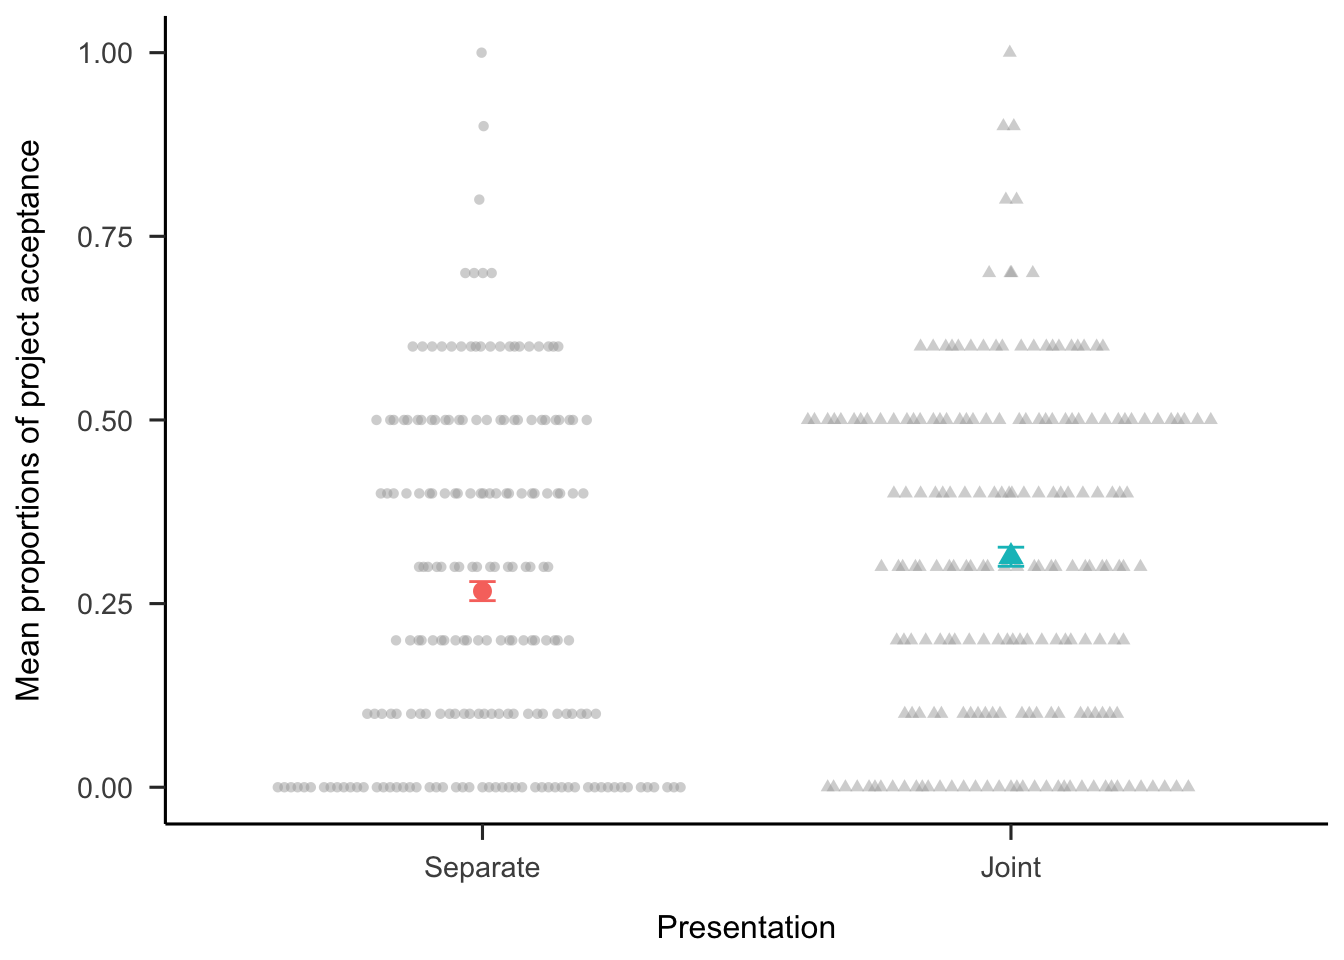
\includegraphics[width=1\linewidth]{thesis_files/figure-latex/plot-aggregation-1-presentation-1} \caption{Mean proportions of decisions to invest in each set of 10 projects, by presentation conditions. Error bars represent 95\% confidence intervals.}\label{fig:plot-aggregation-1-presentation}
\end{figure}



\begin{figure}
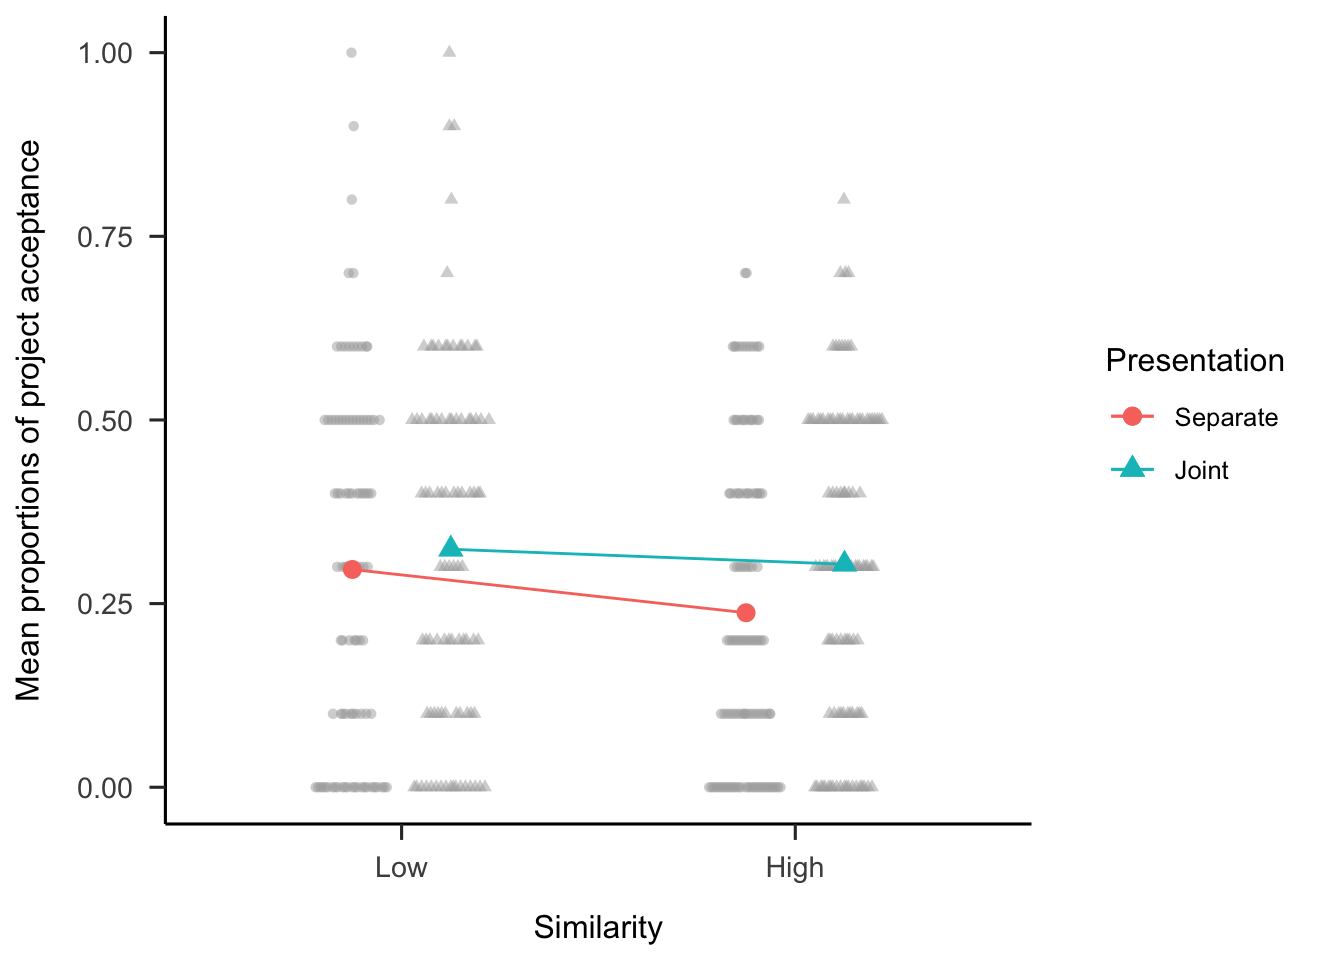
\includegraphics[width=1\linewidth]{thesis_files/figure-latex/plot-aggregation-1-similarity-presentation-1} \caption{Mean proportions of decisions to invest in each set of 10 projects, by similarity and presentation conditions. Error bars represent 95\% confidence intervals.}\label{fig:plot-aggregation-1-similarity-presentation}
\end{figure}

\subsubsection{Trial-by-trial analysis}

Exploratory analyses were conducted into the possible effects of the
manipulations on a trial-by trial basis. The appendix shows the data for all
conditions (see Figure~\ref{fig:plot-aggregation-1-trials}). The key findings
are in the separate presentation. As
Figure~\ref{fig:plot-aggregation-1-trials-separate-awareness} shows, in the
separate condition people are more likely to accept projects over the 10 trials,
but this interacts with awareness,
\(b = 0.04\), 95\% CI \([0.01, 0.08]\), \(z = 2.32\), \(p = .021\).
Specifically, the relationship between choice and trial is stronger in the aware
condition,
\(b = 0.11\), 95\% CI \([0.06, 0.16]\), \(z = 4.54\), \(p < .001\), than in the
naive condition,
\(b = 0.03\), 95\% CI \([-0.03, 0.08]\), \(z = 1.01\), \(p = .311\). It seems that
participants that were told the total number of projects became less risk averse
as the experiment proceeded, regardless of the gamble values.



\begin{figure}
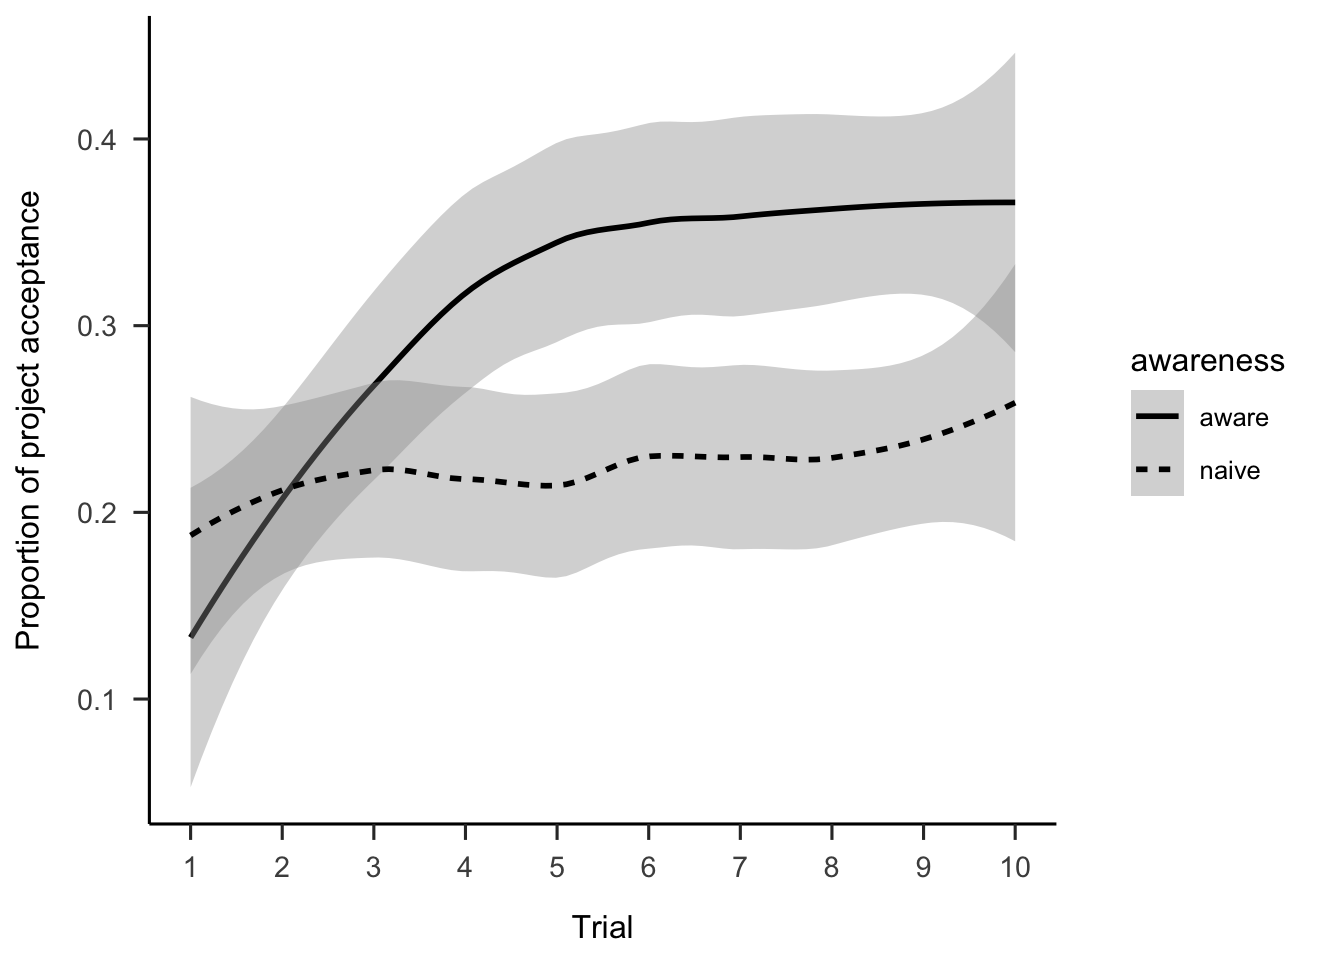
\includegraphics[width=1\linewidth]{thesis_files/figure-latex/plot-aggregation-1-trials-separate-awareness-1} \caption{Proportion of project acceptance in the separate presentation condition, by trial, and awareness conditions. LOESS is used for smoothing over trials and the shading represents 95\% confidence intervals.}\label{fig:plot-aggregation-1-trials-separate-awareness}
\end{figure}

\hypertarget{discussion-aggregation-1}{%
\subsection{Discussion}\label{discussion-aggregation-1}}

Experiment~1 found evidence for most of the hypotheses. Specifically, people
made more risky choices when considering those choices jointly on the same page,
compared to on separate pages; and when they knew how many choices were in the
set. Further, the results showed an interaction between project similarity and
presentation. Exploratory analyses showed that participants' risk aversion
decreased as they proceeded through the trials, but only when participants were
aware of the number of projects.

\subsubsection{Presentation effect}

The presentation effect may be a result of one of two mechanisms. A mathematical
aggregation explanation would mean that participants are combining the gambles
into a mental representation of the probability distribution and then deciding
based on the attractiveness of that distribution. A joint presentation of
choices would facilitate this combination. On the other hand, people may also be
using a sort of naive aggregation process when they are encouraged to group
their choices together. A naive aggregation explanation would suggest that
participants in the joint condition are simply more likely to realise that a few
big wins could offset a few losses. Participants could have been encouraged by
the joint display to consider the set of projects together. This could then lead
to the conclusion that investing in a higher number of gambles might mean that
the gains of some projects will pay off the losses of the other projects.

\subsubsection{Awareness effect}

Experiment~1 found that participants that viewed the projects separately were
more likely to invest in the projects as the trials went on, regardless of the
actual gambles. Having an awareness of the total number of projects in the set
could increase the likelihood that participants would naively aggregate.
Specifically, knowing the number of total projects might increase the salience
of the idea that the gains of some projects will offset the losses of others,
because it reinforces a focus on the entire set. Another possibility is that
participants had a certain aspiration level \autocite{lopes1996} that they were
attempting to reach. This might mean that they invested more as the task
proceeded after realising that the gambles were not becoming significantly more
favourable. \textcite[p.~219]{barron2003} specifically did not tell participants about
the number of gambles they would experience to ``avoid an `end of task' effect
(e.g.~a change in risk attitude).'' \textcite{barron2003} provided participants with
feedback, but this should not be necessary for an aspiration level explanation
since participants only need to be aware of the potential for certain gains.

This result may also be due to a Gambler's fallacy effect or the law of small
numbers. This effect is characterised by people's expectation of a pattern to
follow the underlying distribution of the function that generates each
component. For instance, someone observing the results of a coin flip that look
like HTTHTTTT might anticipate that the likelihood of ``heads'' is higher than
that of ``tails,'' despite the actual likelihood being 50\% for either. This effect
occurs in sequential decision-making, so may be relevant for the repeated-play
decisions in Experiment~1. \textcite{barron2010} found that the gambler's fallacy (in a
roulette prediction task) emerges when information about past outcomes was
displayed sequentially, but not when it is displayed all at once. \textcite{haisley2008}
found evidence for the gambler's fallacy with a repeated-play gamble paradigm.
As such, it is possible that an effect such as the Gambler's fallacy can explain
the effect of the awareness manipulation. That is, participants may have thought
that after a few gambles that they considered risky, the last ones were more
likely to materialise. Further, this would be more likely to occur for those
that knew the total number of projects, because they knew when the sequence was
approaching its end.

\hypertarget{similarity-discussion-aggregation-1}{%
\subsubsection{Similarity effect}\label{similarity-discussion-aggregation-1}}

Experiment~1 did not find a main effect of similarity in the individual choice
data as predicted in Hypothesis~\ref{hyp:similarity-aggregation-1}. Instead,
choice similarity interacted with the presentation condition. This interaction
is harder to explain since it was not hypothesised. In fact, the results seem to
suggest the opposite to what was originally expected. Initially, it was
predicted that people would be less risk averse in the high similarity
condition, due to the better ability to consider the isolated projects as a
grouped set. Similarity was thought to act as a broad bracket, and therefore
increase aggregation. That is, it was expected that seeing a set of similar
projects would help participants aggregate risk when seeing them separately,
more than when projects are dissimilar. Instead, project acceptance was actually
numerically higher in the low than in the high similarity condition
(\(\Delta M = -0.06\), 95\% CI \([-0.12,~0.00]\), \(t(228.14) = -1.83\), \(p = .068\)) when projects were
presented separately, averaging over awareness conditions.

There was no significant difference between similarity conditions regardless of
presentation condition. However, allocations were significantly higher in the
joint presentation condition than in the separate condition for both high and
low similarity. The interaction seems to have been found due to the larger
difference in the high similarity condition. Perhaps the ability to aggregate
risk when projects are presented together is more made more salient when
projects are similar.

Specifically, the interaction seems to be driven by the separate high similarity
condition being lower, rather than by the joint high similarity being higher, as
would have been expected. As such, participants could have been engaged in a
naive \emph{diversification}, rather than a naive aggregation. In ``true''
diversification, people would choose a set of projects that are partially (and
ideally negatively) correlated, as per \textcite{markowitz1952}. However, in reality
people that intend to diversify only seem diversify naively, meaning that they
neglect co-variation when diversifying \autocite[e.g.,][]{hedesstrom2006}. Instead, they
only seem to be looking for variety, rather than diversification in the strict
sense. This \emph{diversification bias} is also seen in product choices \autocite{read1995}.

In Experiment~1, participants may have considered the high similarity condition
as a sign that the set of projects may not be sufficiently ``diversified.''
However, this explanation would also predict the joint presentation condition to
be lower in the high similarity condition. So, perhaps when in the separate
condition, participants were constantly thinking that they might be getting a
different project in the next display, so rejected more projects because of the
lack of diversification, but not realising that they would not be getting any
other type of project. Those in the joint presentation, on the other hand, were
able to see all ten projects, so already knew that there were no other projects
in the set, and so were less likely to reject projects on the basis of the hope
for different projects in the future.

\subsubsection{Limitations}

This experiment had two major limitations. First, proper counterbalancing was
not used in the high alignment project domain, nor in the order of the
within-subjects manipulation of presentation. As such, it is unclear what role
these elements played in the results, especially in the presentation condition,
in which participants always saw the separate condition first. Second, as
mentioned above in Section~\ref{outcome-distribution-materials-aggregation-1},
there was a mistake in the generation of the gamble values that meant that the
individual gambles did not correspond with the distribution that participants
saw. Both of these limitations were addressed in Experiment~2.

\hypertarget{aggregation-2}{%
\section{Experiment~2}\label{aggregation-2}}

Experiment~2 investigated the effect of presentation, awareness, and
distribution on project choice. For the distribution manipulation, half of the
sample saw an outcome probability distribution as in the previous literature
\autocites[e.g.,][]{redelmeier1992,webb2017} to determine their risk aversion when the
gambles are explicitly aggregated. In contrast to most of the repeated-play
choice literature, each choice was presented without subsequent feedback.
Further, in contrast to Experiment~1, the distribution were displayed alongside
each gamble, as opposed to only at the very end. This is an important
manipulation because finding out whether it is effective will 1. add to the
understanding of the conditions necessary for mathematical aggregation (beyond a
mere intuitive sense of aggregation), and 2. suggest new ways to encourage
aggregation in real-world applications.

In past work, participants were shown ordinary binomial distributions, since
multi-play gambles are identical. However, there has not been an investigation
of \emph{non-identical} gamble distributions in this context. Doing this requires
using a \emph{Poisson} binomial distribution, which allows for multiple trials with
different probabilities.

Further, Experiment~2 addressed potential order effects in Experiment~1 by
manipulating all the main variables between-subjects. Manipulating presentation
between-subjects, removes the potentially confounding factor of reduced risk
aversion over time.

Experiment~2 again tested Hypotheses~\ref{hyp:awareness-aggregation-1},
and~\ref{hyp:presentation-aggregation-1}, from Experiment~1. Further, following
the finding in Experiment~1 that participants in the aware condition seemed to
become more risk-taking as the experiment progressed, Experiment~2 tested the
following:

\begin{hypothesis}[Interaction of trial number and awareness]
\protect\hypertarget{hyp:awareness-trials-aggregation-2}{}{\label{hyp:awareness-trials-aggregation-2} \iffalse (Interaction of trial number and awareness) \fi{} }Participants will make more risky choices as the trials progress, but only when
they are aware of the total number of projects in the set.
\end{hypothesis}

Further, multi-play gambles with outcome distributions have been shown to reduce
risk aversion compared to multi-play gambles without distributions \autocites[e.g.,][]{redelmeier1992,webb2017}. Therefore, Experiment~2 tested the following:

\begin{hypothesis}[Distribution effect]
\protect\hypertarget{hyp:distribution-aggregation-2}{}{\label{hyp:distribution-aggregation-2} \iffalse (Distribution effect) \fi{} }Participants will make more risky choices when presented with an aggregated
outcome distribution than when making the same decisions individually.
\end{hypothesis}

\subsection{Method}

\subsubsection{Participants}

One hundred and sixty-four people (51 female) were recruited from the online recruitment platform Prolific. Participants were compensated at a rate of £5 an hour. The average age was 26.39 (\emph{SD} = 8.63, \emph{min} = 18, \emph{max} = 72). Participants reported an average of 2.55 (\emph{SD} = 5.34, \emph{min} = 0, \emph{max} = 43) years of work in a business setting, and an average of 1.67 (\emph{SD} = 2.94, \emph{min} = 0, \emph{max} = 20) years of business education. The mean completion time was 6.53 (\emph{SD} = 5.15, \emph{min} = 1.18, \emph{max} = 39.93) minutes.~Table~\ref{tab:condition-allocation-aggregation-2}
shows the between-subjects condition allocation.
Appendix~\ref{power-analysis-aggregation-2} describes the power analysis
conducted to arrive at this sample size.

\begin{table}[tbp]

\begin{center}
\begin{threeparttable}

\caption{\label{tab:condition-allocation-aggregation-2}Experiment 2 group allocation.}

\begin{tabular}{llll}
\toprule
Awareness & \multicolumn{1}{c}{Distribution} & \multicolumn{1}{c}{Presentation} & \multicolumn{1}{c}{N}\\
\midrule
Aware & Absent & Separate & 40\\
Naive & Absent & Joint & 41\\
Naive & Absent & Separate & 41\\
Naive & Present & Separate & 42\\
Total & - & - & 164\\
\bottomrule
\end{tabular}

\end{threeparttable}
\end{center}

\end{table}

\subsubsection{Materials}

\paragraph{Instructions}

Participants were shown the same instructions as in Experiment~1 (see
Section~\ref{instructions-materials-aggregation-1}).

\hypertarget{task-aggregation-2}{%
\paragraph{Risky investment task}\label{task-aggregation-2}}

Participants saw a similar display to the one in Experiment~1 (see
Section~\ref{task-aggregation-1}), but with new gamble values, in order to fix
the mistake in the Experiment~1 gamble value calculation (detailed in the
appendix Section~\ref{outcome-distribution-aggregation-1}).

The presentation and awareness manipulations were as in Experiment~1. However,
in the distribution-present condition participants saw the outcome probability
distribution of all the projects alongside the description, rather than after
all the projects were seen (see
Figure~\ref{fig:separate-distribution-present-aggregation-2}).



\begin{figure}
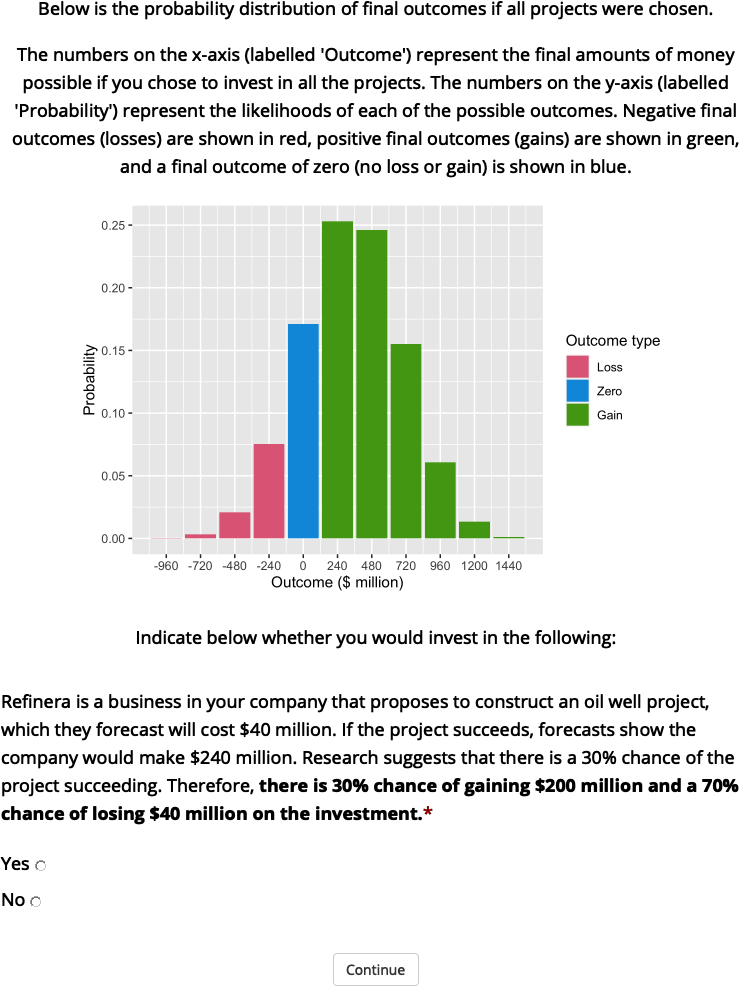
\includegraphics[width=1\linewidth]{thesis_files/figure-latex/separate-distribution-present-aggregation-2-1} \caption{An example of a display seen by those in the separate distribution-present condition of Experiment~2.}\label{fig:separate-distribution-present-aggregation-2}
\end{figure}

\hypertarget{follow-up-aggregation-2}{%
\paragraph{Follow-up}\label{follow-up-aggregation-2}}

Participants were asked how many projects they think they saw, whether they were
willing to accept all or none of the projects, and how many they would be
willing to accept if they had to choose a number.
Appendix~\ref{follow-up-materials-aggregation-2-appendix} shows these
questions.

\subsubsection{Procedure}

Participants read the instructions and completed the risky investment task in
their respective conditions. After seeing the individual projects, participants
were then asked the three follow-up questions.

\hypertarget{results-aggregation-2}{%
\subsection{Results}\label{results-aggregation-2}}

\subsubsection{Project investment}

The project investment data were analysed as proportions of choice per
participant, as in Experiment~1. Each experimental condition was compared to the
same control condition (separate presentation, naive awareness, and distribution
absent). Figure~\ref{fig:plot-aggregation-2-proportion} shows these data. The
difference between presentation conditions was not significant,
\(d_s\) = 0.00, 95\% CI {[}-0.43, 0.43{]}, \(t\)(80) = 0.00, \(p\) = 1.000. Similarly, the
difference between awareness conditions was not significant,
\(d_s\) = 0.15, 95\% CI {[}-0.29, 0.58{]}, \(t\)(79) = 0.66, \(p\) = .508. However, those that that saw a
distribution chose to invest significantly more
(51.19\%) than those that did
not see a distribution
(39.02\%),
\(d_s\) = 0.47, 95\% CI {[}0.03, 0.90{]}, \(t\)(81) = 2.11, \(p\) = .038.



\begin{figure}
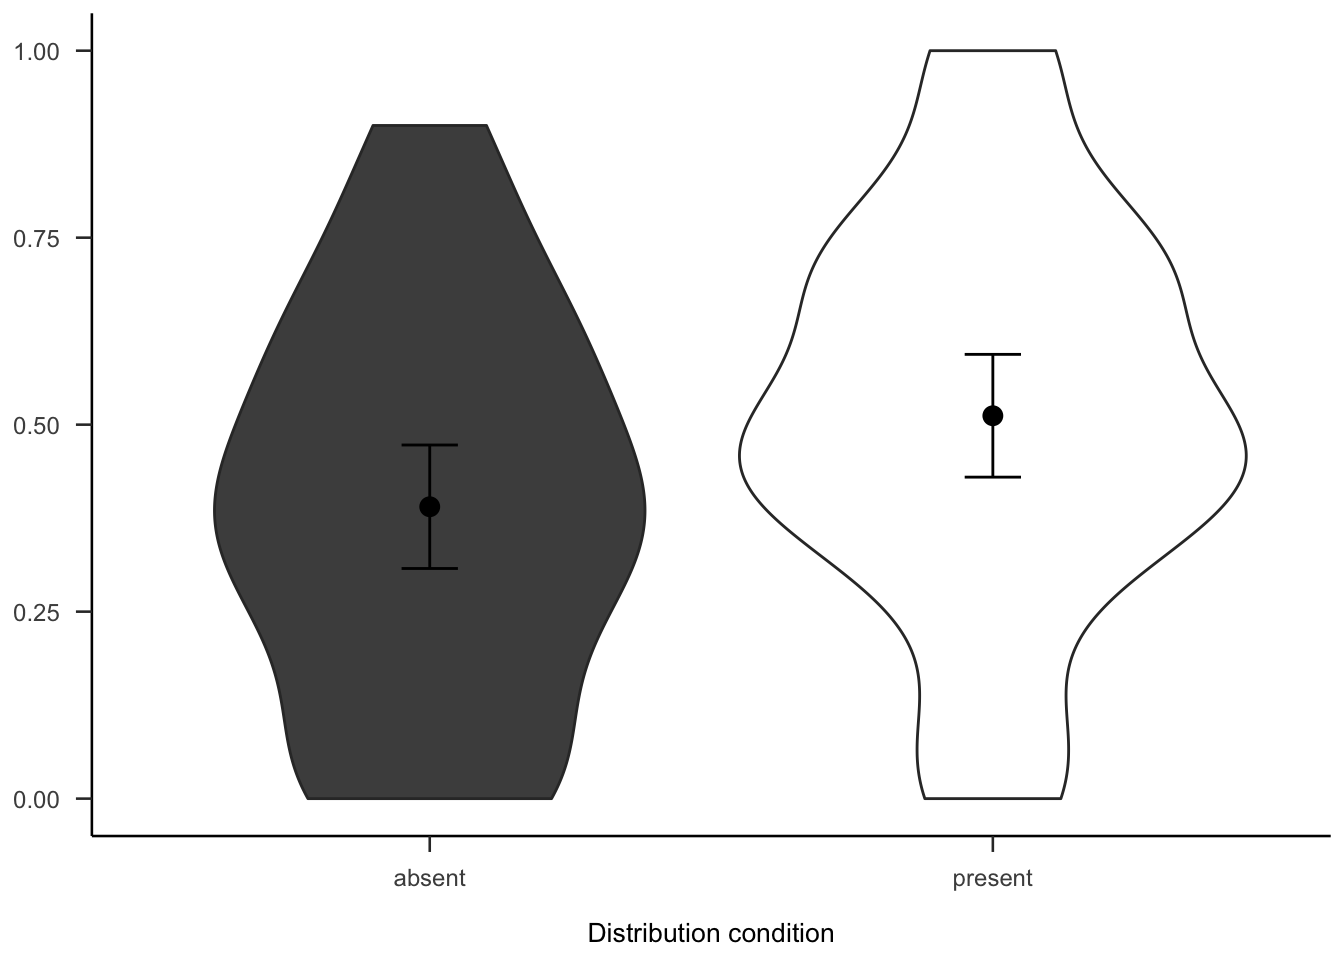
\includegraphics[width=1\linewidth]{thesis_files/figure-latex/plot-aggregation-2-proportion-1} \caption{Mean proportion of project acceptance for the presentation, awareness, and distribution effects. Note, the condition on the left of each effect is the reference condition (separate presentation, naive awareness, distribution absent). As such, it is identical for the three effects. Error bars represent 95\% confidence intervals.}\label{fig:plot-aggregation-2-proportion}
\end{figure}

Further, as Figure~\ref{fig:plot-aggregation-2-choice-trials} shows, it
doesn't seem as if the previous awareness by trial effect was replicated.



\begin{figure}
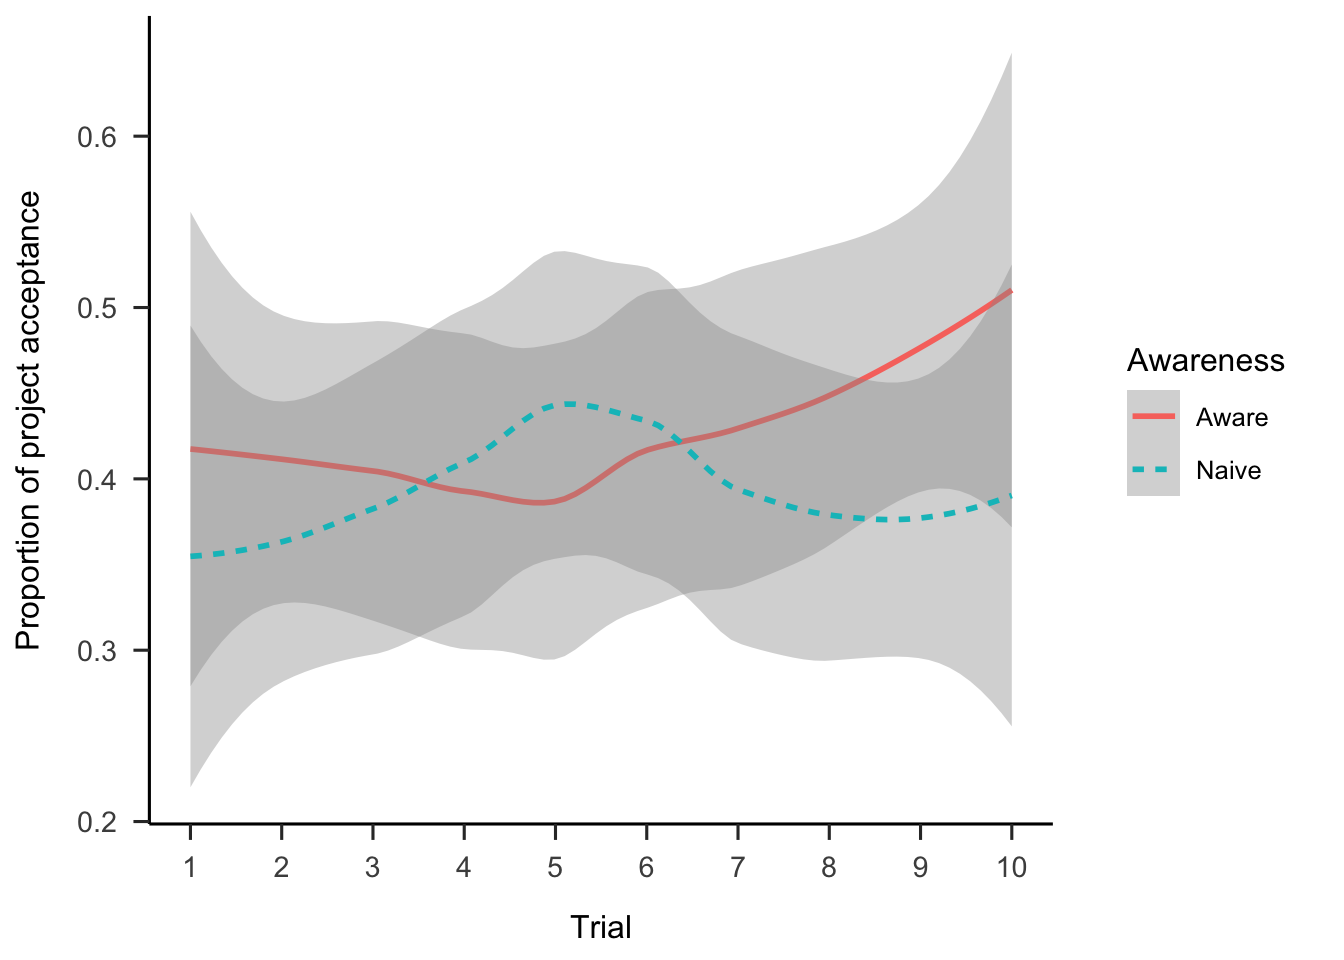
\includegraphics[width=1\linewidth]{thesis_files/figure-latex/plot-aggregation-2-choice-trials-1} \caption{Mean project acceptance for separate presentation, distribution absent condition, by awareness and trial. LOESS is used for smoothing over trials and the shading represents 95\% confidence intervals.}\label{fig:plot-aggregation-2-choice-trials}
\end{figure}

\subsubsection{Follow-up}

The portfolio choice data from both the number and binary questions were
congruent with the above, finding that those in the distribution condition were
more likely to invest (see Appendix~\ref{results-aggregation-2-appendix}).

\hypertarget{discussion-aggregation-4}{%
\subsection{Discussion}\label{discussion-aggregation-4}}

Experiment~2 found support for
Hypothesis~\ref{hyp:distribution-aggregation-2}). Seeing an outcome
distribution of a business project portfolio had a strong effect on
participants' decision-making. Participants indicated that they would invest in
more projects and were more likely to indicate that they would invest in the
entire portfolio. However, the awareness and presentation effects found in
Experiment~1 (see Section~\ref{results-aggregation-1}) did not replicate.

These findings provide evidence for choice bracketing. That is, people do seem
to be primarily considering gambles one at a time. Further, these findings
suggest that that the main bottleneck for appropriately aggregating a set of
gambles is a computational one. That is, people simply cannot mentally combine
the outcomes and probabilities in a way that sufficiently approximates the
outcome distribution display.

The lack of replication of the awareness and presentation effects provides
evidence against a naive aggregation account of the distribution effect.
Specifically this suggests that the distribution effect is a result of a lack of
ability to mathematically combine risk, rather than naive aggregation. If some
of the bottleneck was attributable to a lack of realisation that the individual
gambles could be grouped together, then the effects from Experiment~1 should
have replicated. Instead it seems that even when people have an opportunity to
consider an entire set of risky choices together (and consider that the gains
may outweigh the losses), they do not do this.

In Experiment~2, all the gambles came from the same domain. This was done to
attempt to replicate the relevant effects from Experiment~1. However, there
could have been something about that particular domain that led to the lack of
replication. A follow-up experiment addressed this issue by presenting
participants with 20 gambles from 10 different industries and still did not
replicate the awareness effect (see Appendix~\ref{aggregation-4}).

\section{General discussion}

This chapter found that choice bracketing facilitated risk aggregation in
description-based repeated-play gambles. This paradigm has never been a target
of research. Early work on risk aggregation involved multi-play gambles, which
treated gambles as simultaneous and identical. However, most risky choice
outside the lab involves considering multiple choices independently, as in
repeated-play paradigms. Most repeated-play paradigms have involved providing
participants with feedback, or allowing them to sample from outcome
distributions. Large real-life investments are different, as their outcomes are
not eventuated immediately (and do not allow for distribution sampling). The
limited prior work using description-based repeated-play gambles did not
consider the effect of choice bracketing on risk aggregation. As such, the
paradigm used in this chapter allowed for the investigation of choice bracketing
in a way that is more isomorphic with real-life prescriptions.

Experiment~1 found evidence for the effects of similarity, presentation, and
awareness of the number of projects. Experiment~2 found evidence for the effect
of an outcome distribution but did not replicate the presentation and awareness
effects. Subsequent follow up experiments (reported in
Appendices~\ref{aggregation-3} and~\ref{aggregation-4}) again tested the
similarity and awareness effects. These experiments found evidence for naive
diversification (an advantage for low similarity) when considering them all
projects once and did not replicate the trial-by-trial interaction from
Experiment~1.

Therefore, in addition to the novelty of the paradigm itself, this chapter found
that choice bracketing facilitates risk aggregation. As per
Hypothesis~\ref{hyp:distribution-aggregation-2}, Experiment~2 found that
showing a distribution of outcome probabilities without inter-trial feedback
reduced risk aversion. Further, there was mixed evidence for
Hypothesis~\ref{hyp:similarity-aggregation-1}, such that people were less risk
averse when the set of projects they saw were dissimilar, but only when offered
them as a portfolio (see Appendix~\ref{aggregation-3}). There was only minimal
evidence for Hypotheses~\ref{hyp:awareness-aggregation-1}
and~\ref{hyp:presentation-aggregation-1}, suggesting that viewing projects
together and an awareness of the number of projects are not sufficient to
encourage aggregation. Altogether, it seems that subtle contextual cues are
often not sufficient to encourage risk aggregation and that people need risk to
be is aggregated for them explicitly in order to understand the benefits of
aggregation.

\subsection{Theoretical implications}

The finding that participants are less risk averse when provided with an
aggregated outcome distribution is congruent with previous work \autocite[e.g.,][]{redelmeier1992}. However, when distributions have been previously used, gambles
were identical---as in multi-play paradigms---and used immediate feedback for
repeated-play paradigms \autocite[e.g.,][]{benartzi1999}. As mentioned previously, both
these paradigms have limited ecological validity because usually people are
faced with non-identical sequential choices and do not receive immediate
feedback. This work is the first to provide evidence for this aggregation effect
with non-identical gambles without feedback.

The other choice bracketing findings are less congruent with previous research.
\textcite{sokolhessner2009} and \textcite{sokolhessner2012} found that encouraging participants to
make decisions akin to a professional investor increased the amount of risky
choices they made. The results showed that a subtler manipulation---whether or
not participants were aware of the number of choices to be made---is not
sufficient to encourage aggregation. \textcite{hsee1999} found that useful, but
hard-to-interpret, attributes were used more when the options were presented
jointly, rather than separately. In the case of these experiments, the ``hard to
interpret'' element of the decision set was the risk of the projects. Contrary to
\textcite{hsee1999}, it seems that risk was not always accounted for more when projects
were presented jointly, rather than separately. More study is needed to
understand whether the effects that were seen in Experiment~1 but not replicated
in the subsequent experiments are due to statistical chance or specific elements
of the experiment.

Research on the effect of option similarity on choice \autocite[e.g.,][]{markman1995}
suggests that alignable differences are more important than non-alignable
differences. Further, the effects of multi-play gambles and outcome
distributions on risk aggregation are only seen when participants perceive the
options as fungible \autocite[e.g.,][]{dekay2005}. As such, it was predicted that a set of
investments that involve the same type of investment would be seen as more
similar, and therefore be considered as fungible.
Hypothesis~\ref{hyp:similarity-aggregation-1} predicted that this would
facilitate a broad bracketing, and therefore more risk aggregation.

Instead, the results showed that choice similarity did not affect individual
project allocations. However, when participants were given an all-or-nothing
choice for the entire set of projects, those that viewed dissimilar projects
were more likely to take the entire set projects than those that viewed similar
projects. This is different from the initial hypothesis, however, it may still
suggest an effect of choice bracketing. That is, this effect was only found when
participants were asked about the entire portfolio of projects, rather than when
they had a chance to make a choice about each project. The way that the question
was framed may have acted to broadly bracket the choices by forcing the choice.

A diversified portfolio is one whose investments are uncorrelated or negatively
correlated. According to Portfolio Theory \autocite{markowitz1952}, a diversified
portfolio is preferred to one that is not diversified, because it reduces the
probability of a loss. When some investments have losses, others will have
gains---the root of ``don't keep all your eggs in one basket.'' Typically,
questions of gamble aggregation assume that each gamble is independent. That is,
the gambles are uncorrelated. As such, aggregation of a portfolio already
assumes that the portfolio is somewhat diversified (or at least that the gambles
aren't perfectly correlated).

In the case of the similarity effect, the choice bracketing did not seem to
encourage aggregation, but instead appears to have encouraged a naive
diversification \autocite{hedesstrom2006,read1995}. It could not have been actual
diversification, because the projects did not contain correlational information.
Instead, participants could have been more eager to accept the project portfolio
due to the higher variability between projects (due to the similarity
manipulation).

\subsubsection{How does choice bracketing facilitate aggregation?}

Much of the literature \autocite[e.g.,][]{benartzi1999} is not clear about why choice
bracketing occurs. Some explain the effect of bracketing on aggregation using
risk aversion \autocite[e.g.,][]{read1999}, while others refer to the increased weighting
of potential losses \autocite{webb2017}.

Decision-from-experience \emph{sampling} studies explain the underweighting of rare
events (as opposed to the overweighting that occurs with
decisions-from-description) by sampling bias and recency effects \autocites[e.g.,][]{hertwig2004,wulff2018}. That is, they explain that people are less risk
averse for positive EV gambles because when they sample from the distribution
they only sample a small amount (usually approximately 20 times) so they do not
experience rare events very often. Also, the latter half of the sequence of
sampling is significantly more predictive than the former (recency effect). Some
decision-from-experience \emph{feedback} studies explain this effect by ``choice
inertia'' \autocite{camilleri2011}. That is, ``the tendency to repeat the last choice,
irrespective of the obtained outcome'' (p.~383). However, there is not much more
elaboration beyond this. Repeated-play gambles show more underweighting than
multi-play gambles. This is said to be due to a ``reliance on a very small set of
samples'' \autocite[p.~64]{camilleri2013}. However, this explanation does not account for
repeated-play effects independently.

The experiments in this chapter shed some light about the mechanisms behind why
choice bracketing may affect risk aggregation in repeated-play gambles without
feedback. Two explanations were proposed: participants may realise that some
gains will offset the losses, or they may need explicit aggregation. Not finding
evidence for the subtle choice bracketing manipulations suggests that people do
not intuitively consider that the gains of their choices may offset the
potential losses. Perhaps the possibility of recouped losses would become more
salient when other participants are explicitly told of this possibility, as in
\textcite{sokolhessner2009}. Their explicit instruction manipulation is introduced above
as appearing unrealistically strong, but the results of this chapter suggest
that people do need very explicit scaffolding in order to use risk aggregation.

\subsection{Practical implications}

This research implies some prescriptions for capital allocation decision-making.
For instance, even if managers implement processes that encourage a joint
evaluation of projects, this may be insufficient to encourage aggregation.
Projects need to very explicitly be considered as individual components in a
portfolio in order to facilitate better risk aggregation. Some companies are
already implementing processes that make this more explicit \autocite{lovallo2020}. This
is especially important for those that would still have to evaluate projects
separately. Further, this work shows the importance of being explicit about the
forecasted probabilities of project success. Doing this is necessary for the
aggregation process. Even more ideal would be to forecast project success using
an entire probability distribution for the different possible outcomes. However,
research shows that people struggle to construct such distributions \autocites[e.g.,][]{alpert1982,schaefer1973,staelvonholstein1971,tversky1974} and
Chapter~\ref{alignment} shows that people struggle to use such variance
information when making allocation decisions.

Interestingly, participants were less risk averse about a portfolio of projects
when industries differed, compared to when they were all from the same industry.
Simply manipulating the similarity of financially-irrelevant semantics of a set
of choices affected participants' risk aversion. This has implications for
managerial settings. Executives in multi-business firms often have to make
capital allocation decisions that involve comparing dissimilar projects. How can
an oil well exploration project be appropriately compared to an oil refinery? Or
to a microchip project? Chapter~\ref{alignment} suggests that evaluating
dissimilar business projects is more difficult to comparing similar projects.
The current work suggests that managers may actually be \emph{less} likely to realise
the benefits of aggregation when they are in a less diversified company. As
such, managers should complement an understanding of aggregation with that of
diversification. This might help to avoid being biased by a lack of variety of
projects despite a potentially high level of diversification.

\subsection{Future research}

The main novelty of the experiments in this chapter comes from increasing
ecological validity of risky choice problems by removing inter-trial feedback.
Future work should test even more realistic scenarios. Such studies should
involve managers, ideally in multi-business firms. Investigating whether the
choice bracketing findings from these experiments replicates in a sample of
managers will help to determine whether these results could be applied to
real-world managerial decision-making. This is especially important since
\textcite{haigh2005} found that professional traders show more myopic loss aversion than
students. Further, the similarity, awareness, and presentation manipulations
should be tested with managers since it is possible that they have a greater
sense of naive aggregation and are therefore more likely to be more amenable to
such manipulations. The addition of extra payment for better performance on the
task might also assist in making the task more isomorphic with real-world
managerial decisions. Further, in the present experiments, participants viewed
the projects all in the space of one session. However, this is not completely
isomorphic to real life, where managers make many other decisions that are
unrelated to the large risky investments at their companies. Future research
should test participants over a longer period of time \autocite[as in][]{beshears2016} in
order to see whether the effects of the manipulations replicate in a more
realistic environment.

\newpage

\printbibliography[segment=\therefsegment,heading=subbibintoc]

\hypertarget{interstitial-1}{%
\chapter{Joint evaluation of multiple projects}\label{interstitial-1}}

Chapter~\ref{aggregation} found that people struggle to aggregate risk even
when provided with choice bracketing cues that could have built on an intuitive
sense of how aggregation reduces risk. The finding that people are more likely
to accept many gambles at once \autocites[e.g.,][]{samuelson1963,wedell1994}, even without
any aids to calculate risk, suggests that people can gain an intuition for the
benefits of aggregation. Yet, in the current work, people instead considered
projects one at a time and only leveraged the benefits of aggregation when given
an explicit visualisation of what it entails.

This shows that it is important to change organisational policy to encourage
considering business projects jointly. Doing this means that the risk can be
concurrently aggregated. In real-life capital allocation scenarios, when
managers evaluate projects sequentially, an aggregated distribution can also be
presented using any number of projects that were considered in the recent past.
This means that a strategy of project risk aggregation can be implemented at any
stage in an organisation's lifespan. Relatively new ventures can implement these
recommendations by waiting until a certain number of project proposals have been
accrued before aggregating.

Considering projects jointly is also useful for accountability purposes. The
usual incentive structure in organisations that judges each project outcome
independently is likely to punish risk-taking due to its potential negative
consequences and not due to the information that was available at the time of
evaluation. Framing a set of projects as a portfolio means that any subsequent
success or failure of one project can be traced back to the entire batch, and
the performance of the whole portfolio can be evaluated.

Business projects might not always be either accepted or rejected, as in
Chapter~\ref{aggregation}. Instead, top-level managers might ask for project
proposals from lower-level managers, and then allocate funds from the available
budget. An organisation might also have a initial ``culling'' phase, and a
subsequent ranking phase. When initially considering a set of projects, some
might be rejected according to certain rules. For instance, an NPV might not
meet a certain minimum cut-off. The remaining projects in the set can then be
ranked in order of priority and receive an allocation of capital from the
budget.

A few potential problems arise at the point that projects are considered jointly
for ranking and allocation. For instance, it might not be easy to compare
between the projects in the set. As discussed in Chapter~\ref{introduction},
diversification of business units has become very popular in large
organisations. Therefore, most hierarchical organisations are likely to face
difficult comparisons when deciding on how to rank and allocate capital to
projects that originated in different divisions. A non-hierarchical organisation
that develops one type of product may be able to simply compare across any
number of intrinsic project attributes, whereas a diversified organisation is
likely to have to rely on more abstract financial metrics, such as NPV. Such
metrics are ``abstract'' because they can be applied in almost any domain.

For instance, when comparing across two oil well projects, there can be both
attributes intrinsic to the project, such as the amount of hydrocarbons that are
extracted per hour, and also the more abstract financial metrics. There is a
potential interaction between the ease that managers have to compare across the
projects and the kinds of measures that are used to make the comparison. Two
similar projects, such as two oil wells can be evaluated using litres of
hydrocarbons extracted per hour, whereas an oil refinery cannot. In the case
that two dissimilar projects are compared, managers can use financial metrics to
compare across domains. This can lead to comparable accuracy as long as the
abstract metrics are as reliable as the intrinsic project features.

A concern that arises out of a reliance on such metrics is that underlying
variance is not taken into account. Forecast estimates such as NPV rely on many
assumptions and contain much inherent uncertainty, so managers that use them
should be cautious about over-relying on them. Chapter~\ref{alignment} tested
people's sensitivity to forecast estimate variance information. That is, will
people use NPV more when the variance information suggests that it is a reliable
measure, than when the information suggests that it is unreliable?

Chapter~\ref{aggregation} manipulated project presentation and found no
significant difference between when projects were considered jointly or
separately. This was explained by the bounds on people's ability to intuitively
aggregate. However, it was unclear what components of the projects people
focused on both because they were not explicitly manipulated and because the
task involved a binary choice (accept or reject). A relative allocation measure
for multiple projects with systematically varied attributes would allow to
determine the influence of those different attributes. Therefore,
Chapter~\ref{alignment} considered the situation in which people are already
presented with choices together and asked to evaluate the projects by allocating
a hypothetical budget.

Further, Chapter~\ref{alignment} identified the factors that affect people's
decisions independently from the potential risk of losing hypothetical money,
which is a large reason for the effects in the previous chapter. Risk aversion
was accounted for by making it clear that no losses are possible. This was
achieved by using only positive NPVs, which implies that the project is not
forecasted to lose money.

Chapter~\ref{alignment} also manipulated how easy the project attributes are to
compare in order to identify the ways that decision-making in a diversified
organisation might be different to that of a more integrated organisation.
Chapter~\ref{aggregation} manipulated similarity by either showing a set of
projects from the same industry or a set from different industries. This was
meant to simulate an integrated and diversified firm, respectively. This
manipulation was not as strong because there were no project attributes that
could be aligned or not. That is, there was nothing actually non-alignable. This
may explain the equivocal similarity effect. Chapter~\ref{alignment} more fully
manipulated alignability by having project attributes be critical to the
evaluation. These project features were shown explicitly so that the difficulty
of the comparison is more obvious.



\begin{savequote}
It is not possible to compare apples and oranges. But it is possible to
compare apples and oranges in terms of some specific attribute---to say
that apples deliver twice as many calories per dollar or that oranges
deliver twice as many vitamin C units per dollar.
\qauthor{---\textcite[p.~13]{robinson1944}}\end{savequote}

\hypertarget{alignment}{%
\chapter{Project similarity bias and variance neglect in forecast metric evaluation}\label{alignment}}

\minitoc

\section{Introduction}

One of the most important tasks that executives face is allocating capital
within their company. This requires ranking different projects based on their
importance and predicted success, and allocating limited capital respectively
(not unlike a scientific funding agency). Ranking projects requires comparing
them across a number of dimensions. For example, an executive in an oil company
might have multiple proposals on his or her desk for where to explore for oil
next and how to do so. Figuring out what makes one oil discovery project better
than another one is relatively easy. However, consider a different scenario in
which the executive has to allocate capital between an oil discovery project
and an oil refinery project. The dimensions of an oil refinery project that
distinguishes good from bad projects may be totally different from the
dimensions of oil discovery projects that do the same. Think of a funding agency
giving out fellowships and deciding between two cognitive scientists, or a
cognitive scientist and a physicist. What makes a physics proposal better for
the field of physics than a cognitive science proposal is for cognitive science?

Structure-mapping theory \autocites[SMT;][]{gentner1997,gentner1983} provides a model of
comparison that psychologically distinguishes these two kinds of allocation
tasks. SMT models comparison as a process of bringing conceptual structures into
alignment which, when possible, puts shared component dimensions into
correspondence. Alignment both highlights when two conceptual structures share
dimensions, and also highlights how the two structures differ along those shared
dimensions, called \emph{alignable differences}. For example, when comparing two oil
discovery projects, all the relevant processes of planning an exploration and
measuring the amount of hydrocarbons in a prospect might be identical, but the
specific amount measured will be different. This is the alignable difference: a
difference between the two projects that is constrained within the same
conceptual structure. However, when comparing between an oil field and a
refinery, there will be significantly more \emph{non-alignable differences}, because
the two domains do not share component dimensions. That is, many of the
processes that exist in the exploration business unit have a significantly
different dimensional structure to those in the refinery business unit, such
that it will be difficult to find meaningful alignments. More non-alignable
differences mean that there are less opportunities to make meaningful
comparisons, and so would make predicting project success and ranking their
priority more difficult. This chapter experimentally examined project
comparisons and how such comparisons affect capital allocation decisions. The
working hypothesis was that comparisons with more alignable differences will
make project predictions more precise, and project rankings easier and more
informative, than a comparison with non-alignable differences.

However, what happens when the two domains are too disparate for a
decision-maker to align them, but the task demands that they be aligned? This is
actually a bit of uncharted territory experimentally. The prediction is that
when forced to, people will grab at any piece of information that they can and
then try to infer and abstract as much as seems reasonable to ease the
alignment. This is in fact what occurs very frequently in business settings.
Corporate enterprises continue to embrace diversification strategies in their
investments, and so constantly have to make capital allocation choices that
involve very disparate domains. To overcome these difficult comparisons,
executives rely on various financial measures that in theory can apply to any
project or business proposal. These financial measures work well to ease the
burden of the difficult comparison by abstracting away from the complexities of
the individual projects, and just focus on financial information such as total
costs, projected profits, etc. Initially hard-to-compare projects can therefore
be more easily evaluated by comparing values on individual numerical measures.

The most common financial measure that is used by executives in order to value
business project proposals is Net Present Value \autocites[NPV;][]{graham2001,remer1993,graham2015}. NPV is the difference between the money that a project is
forecasted to make and the initial investment in its development (accounting for
the time value of money), as seen in Equation~\eqref{eq:npv}.

NPV is commonly used to decide about capital allocation and investment. The
simple rule is that if a project's NPV is positive, then it is financially
viable, and if NPV is negative, then it is not. However, the use of NPV has been
criticised, both by academics and practitioners \autocite{fox2008,willigers2017}. The
main criticism is that there is underlying variance within the NPV measure that
is not made apparent by the final form of the measure, a single numerical value.
For instance, NPV is dependent on the cash inflows that are projected for each
year of the project. However, financial forecasting is known to often be
inaccurate and prone to optimism bias \autocite{lovallo2003,puri2007}. Therefore,
there is bound to be variation in the reliability of NPV measures as a function
of the forecasting error in the cash flow calculations. The duration of the
project and the discount rate are further sources of variance that are hidden by
the single numerical value of NPV.

As such, the secondary goal of this research was to investigate the extent to
which people are sensitive to variance information (from financial forecasting)
when making capital allocation decisions. This consideration is especially
important in the capital allocation situations illustrated above, in which
executives need to compare between projects from disparate domains and therefore
have to rely on NPV. This matters because the NPV calculated from different
domains may have different underlying forecasting error, which may compromise
the utility of using NPV as the basis of the comparison. Do executives
sufficiently account for the inherent variance in the measure that they rely on
so much? Research shows that people are good at extracting variance information
when experiencing numerical sequences \autocite{rosenbaum2020}. However, people struggle
to use variance information when it is represented numerically \autocite{galesic2010,konold1993,vivalt2021,batteux2020}.

\subsection{Experiment summary}

Experiment~1 investigated the effect of alignment on the decision-making of
naive participants' capital allocation to a set of fictional projects. NPV
reliability was manipulated by directly stating whether it is a reliable measure
because the naive participants were assumed not to have the requisite knowledge
to be sensitive to reliability information otherwise. This experiment predicted
that when projects are alignable, participants use NPV if they are told that it
is a reliable measure, but do not use it if they are told that it is unreliable.
However, when projects are not alignable, participants were predicted to use NPV
regardless of the stated NPV reliable.

Experiment~2 investigated the decision-making of management students in almost
the same situation as Experiment~1. The main difference was that instead of
telling participants the reliability of NPV, this experiment manipulated the
level of associated \emph{numerical} NPV reliability. That is, the width of numerical
ranges around an NPV. Participants were predicted to rely more on NPV in the
non-alignable projects than in the alignable projects. However, this experiment
predicted that there will be no effect of numerical reliability, since there is
very little evidence that people are sensitive to variance information when
represented numerically.

Experiment~3 again tested the alignment and reliability effects in a
non-business population, but manipulated both verbal and numerical reliability
in the same experiment to allow for direct comparisons. An effect of reliability
was predicted in the verbal reliability condition, but not in the numerical
reliability condition. Further, this experiment used project descriptions with
clearer profitability indicators, and added a larger selection of business
industries.

\hypertarget{alignment-2}{%
\section{Experiment~1}\label{alignment-2}}

Experiment~1 investigated the effects of alignment and explicit NPV reliability
information on capital allocation decisions. The structural alignment literature
suggests that people weigh alignable differences more heavily than non-alignable
differences. It was expected that people would use NPV more than any other
product attributes (because it applied to every product). However, this effect
should vary with participants' perceived reliability of the value. That is, if
other project dimensions were alignable, then it should be easier to adjust the
use of NPV based on its reliability. However, it was predicted that in low
alignment there will be a reliance on NPV, as the sole alignable difference,
regardless of its stated reliability. These effects were measured by considering
the linear trend of how NPV, across projects, relates to the money allocated to
the projects. Critically, participants saw both NPV and other features intrinsic
to each project domain, and these were inversely related. Therefore, a positive
NPV amount trend indicated a reliance on NPV, whereas a negative trend indicated
a reliance on the intrinsic project features. First, Experiment~1 tested the
following omnibus hypothesis:

\begin{hypothesis}[Overall effect]
\protect\hypertarget{hyp:three-way-alignment-2}{}{\label{hyp:three-way-alignment-2} \iffalse (Overall effect) \fi{} }The alignment \(\times\) reliability amount \(\times\) NPV amount interaction will
be significant.
\end{hypothesis}

Initially, the specific effects were tested excluding the no NPV condition.
Comparing across dissimilar projects will be difficult, so participants are
expected to rely on NPV more in such a scenario than when they have other
alignable attributes. Therefore, Experiment~1 tested the following:

\begin{hypothesis}[Alignment effect]
\protect\hypertarget{hyp:allocation-alignment-alignment-2}{}{\label{hyp:allocation-alignment-alignment-2} \iffalse (Alignment effect) \fi{} }The linear NPV amount trend will be higher, on average, in low alignment
than in high alignment.
\end{hypothesis}

Participants are likely to moderate their allocations based on the provided
reliability information. However, it is more likely that they will do this when
they have multiple options for metrics to use than when only NPV is
alignable. Therefore, Experiment~1 tested the following:

\begin{hypothesis}[Moderation of NPV reliability by alignment]
\protect\hypertarget{hyp:allocation-alignment-reliability-npv-alignment-2}{}{\label{hyp:allocation-alignment-reliability-npv-alignment-2} \iffalse (Moderation of NPV reliability by alignment) \fi{} }The NPV amount \(\times\) reliability interaction will be stronger in the high
alignment than in low alignment.
\end{hypothesis}

More specifically, it is expected that when projects are similar, participants
will rely on NPV more (positive NPV amount trend) when they are told that it is
reliable and rely more on the projects' intrinsic features (negative NPV amount
trend) when they are told that it is unreliable. However, when projects are
dissimilar, it is expected that participants will rely solely on NPV solely,
regardless of what they are told about its reliability. Therefore, Experiment~1
tested the following:

\begin{hypothesis}[NPV reliability in high alignment]
\protect\hypertarget{hyp:allocation-alignment-high-alignment-2}{}{\label{hyp:allocation-alignment-high-alignment-2} \iffalse (NPV reliability in high alignment) \fi{} }In high alignment, the linear NPV amount trend will be higher in
the high reliability condition than in the low reliability condition
\end{hypothesis}

\begin{hypothesis}[NPV reliability in low alignment]
\protect\hypertarget{hyp:allocation-alignment-low-alignment-2}{}{\label{hyp:allocation-alignment-low-alignment-2} \iffalse (NPV reliability in low alignment) \fi{} }In low alignment, the linear NPV amount trend will not differ
significantly between reliability conditions
\end{hypothesis}

A no NPV condition was used to gain a better understanding of the baseline
responding to the materials without NPV. This was used to determine the extent
of participants' reliance on NPV. When projects were similar, this condition was
expected to be equivalent to the low reliability condition, as participants
disregard NPV. When projects were dissimilar, this condition was expected to
express the average participant value judgements for the project descriptions,
which should result in a more or less flat NPV amount trend. Therefore,
Experiment~1 tested the following:

\begin{hypothesis}[No NPV comparison in high alignment]
\protect\hypertarget{hyp:allocation-alignment-high-no-NPV-alignment-2}{}{\label{hyp:allocation-alignment-high-no-NPV-alignment-2} \iffalse (No NPV comparison in high alignment) \fi{} }In high alignment, the linear NPV amount trend will be higher in the high
reliability condition than in the no NPV reliability condition.
\end{hypothesis}

\begin{hypothesis}[No NPV comparison in low alignment]
\protect\hypertarget{hyp:allocation-alignment-low-no-NPV-alignment-2}{}{\label{hyp:allocation-alignment-low-no-NPV-alignment-2} \iffalse (No NPV comparison in low alignment) \fi{} }In low alignment, the linear NPV amount trend in both the low and high
reliability conditions will be higher than the no NPV reliability condition.
\end{hypothesis}

\subsection{Method}

\subsubsection{Participants}

One hundred and eighteen people (55 female) were recruited from the online recruitment platform Prolific. Participants were compensated at a rate of £5 an hour. The average age was 29.42 (\emph{SD} = 9.25, \emph{min} = 18, \emph{max} = 73).~Table~\ref{tab:condition-allocation-alignment-2}
shows the between-subjects condition allocation. NPV amount was varied within
subjects.

\begin{table}[tbp]

\begin{center}
\begin{threeparttable}

\caption{\label{tab:condition-allocation-alignment-2}Experiment 1 group allocation.}

\begin{tabular}{lll}
\toprule
Alignment & \multicolumn{1}{c}{Reliability amount} & \multicolumn{1}{c}{N}\\
\midrule
High & High & 26\\
High & Low & 17\\
High & No NPV & 17\\
Low & High & 21\\
Low & Low & 16\\
Low & No NPV & 21\\
Total & - & 118\\
\bottomrule
\end{tabular}

\end{threeparttable}
\end{center}

\end{table}

\hypertarget{materials-alignment-2}{%
\subsubsection{Materials}\label{materials-alignment-2}}

\hypertarget{instructions-materials-alignment-2}{%
\paragraph{Instructions}\label{instructions-materials-alignment-2}}

The instructions page explained to the participants, who did not necessarily
have business experience, about the task and NPV. However, this page was also
used to manipulate whether participants were told that NPV was reliable or
unreliable as a financial measure. Participants in the low NPV reliability
condition were told that NPV is an unreliable metric, whereas those in the high
NPV reliability condition were told that NPV is a reliable metric. Those in the
no NPV condition saw instructions that did not include the NPV explanation.
Critically, participants were told to invest in products with a high objective
value (because a better quality product is not always better in a consumer goods
market). Since participants might still not use this instruction when directly
viewing the projects, Experiment~3 used projects with attributes that more
inherently conveyed quality.
Appendix~\ref{instructions-materials-alignment-2-appendix} shows the
instructions used in Experiment~1.

\hypertarget{projects-materials-alignment-2}{%
\paragraph{Project display}\label{projects-materials-alignment-2}}

Participants read sets of fictional business projects for which to potentially
allocate capital. The high alignment display was a table that listed various
attributes for five projects (see
Figure~\ref{fig:projects-alignment-high-materials-alignment-2}). The low
alignment display presented each project as individual paragraphs that described
the relevant attributes with full sentences (see
Figure~\ref{fig:projects-alignment-low-materials-alignment-2}). In the high
alignment display, all projects were of the same product type and the concrete
attributes were consistent. In the low alignment display, each project was of a
different product with concrete attributes relevant to that project. For both
alignment conditions, each project description included an NPV.

This alignment manipulation was reinforced by visual presentation. The table
format was better afforded by the high alignment condition because all the
dimensions were shared. However, this confounded alignment with presentation
style. This was addressed in Experiment~3 by equating the table format across
both alignment conditions.



\begin{figure}
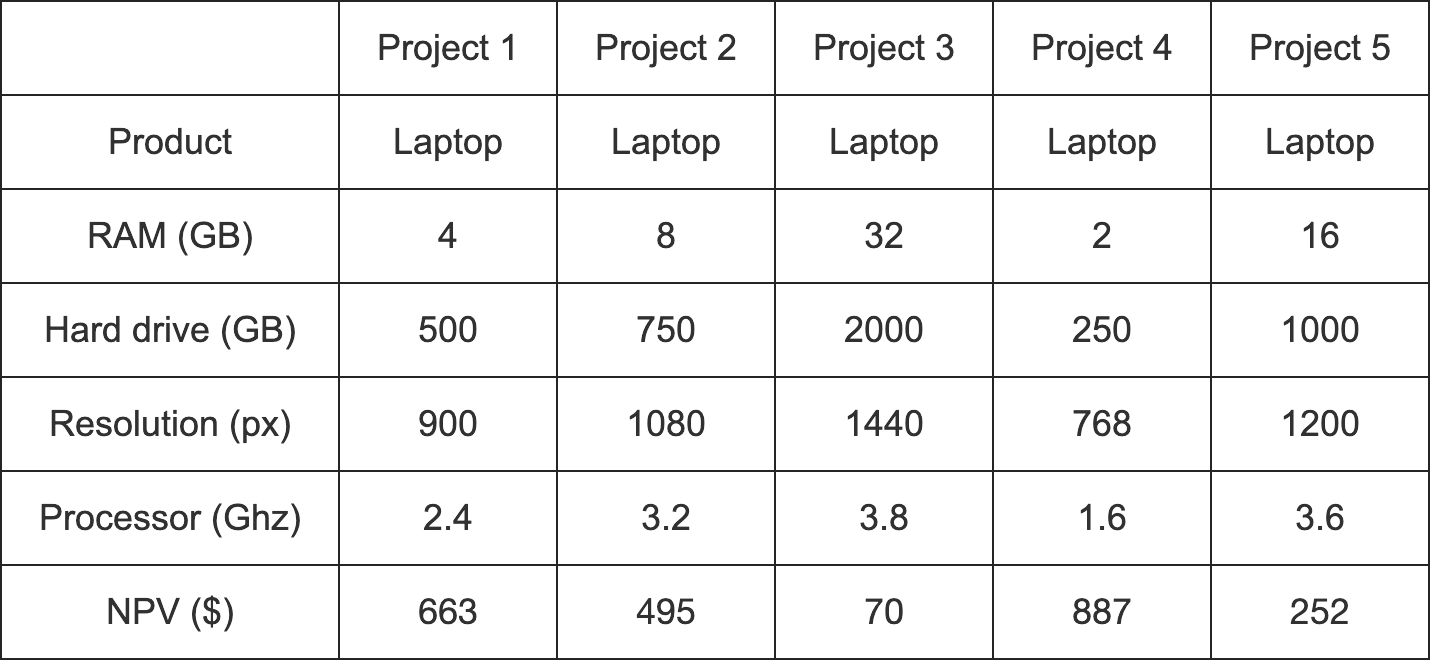
\includegraphics[width=1\linewidth]{thesis_files/figure-latex/projects-alignment-high-materials-alignment-2-1} \caption{An example of a high alignment display in Experiment~1.}\label{fig:projects-alignment-high-materials-alignment-2}
\end{figure}



\begin{figure}
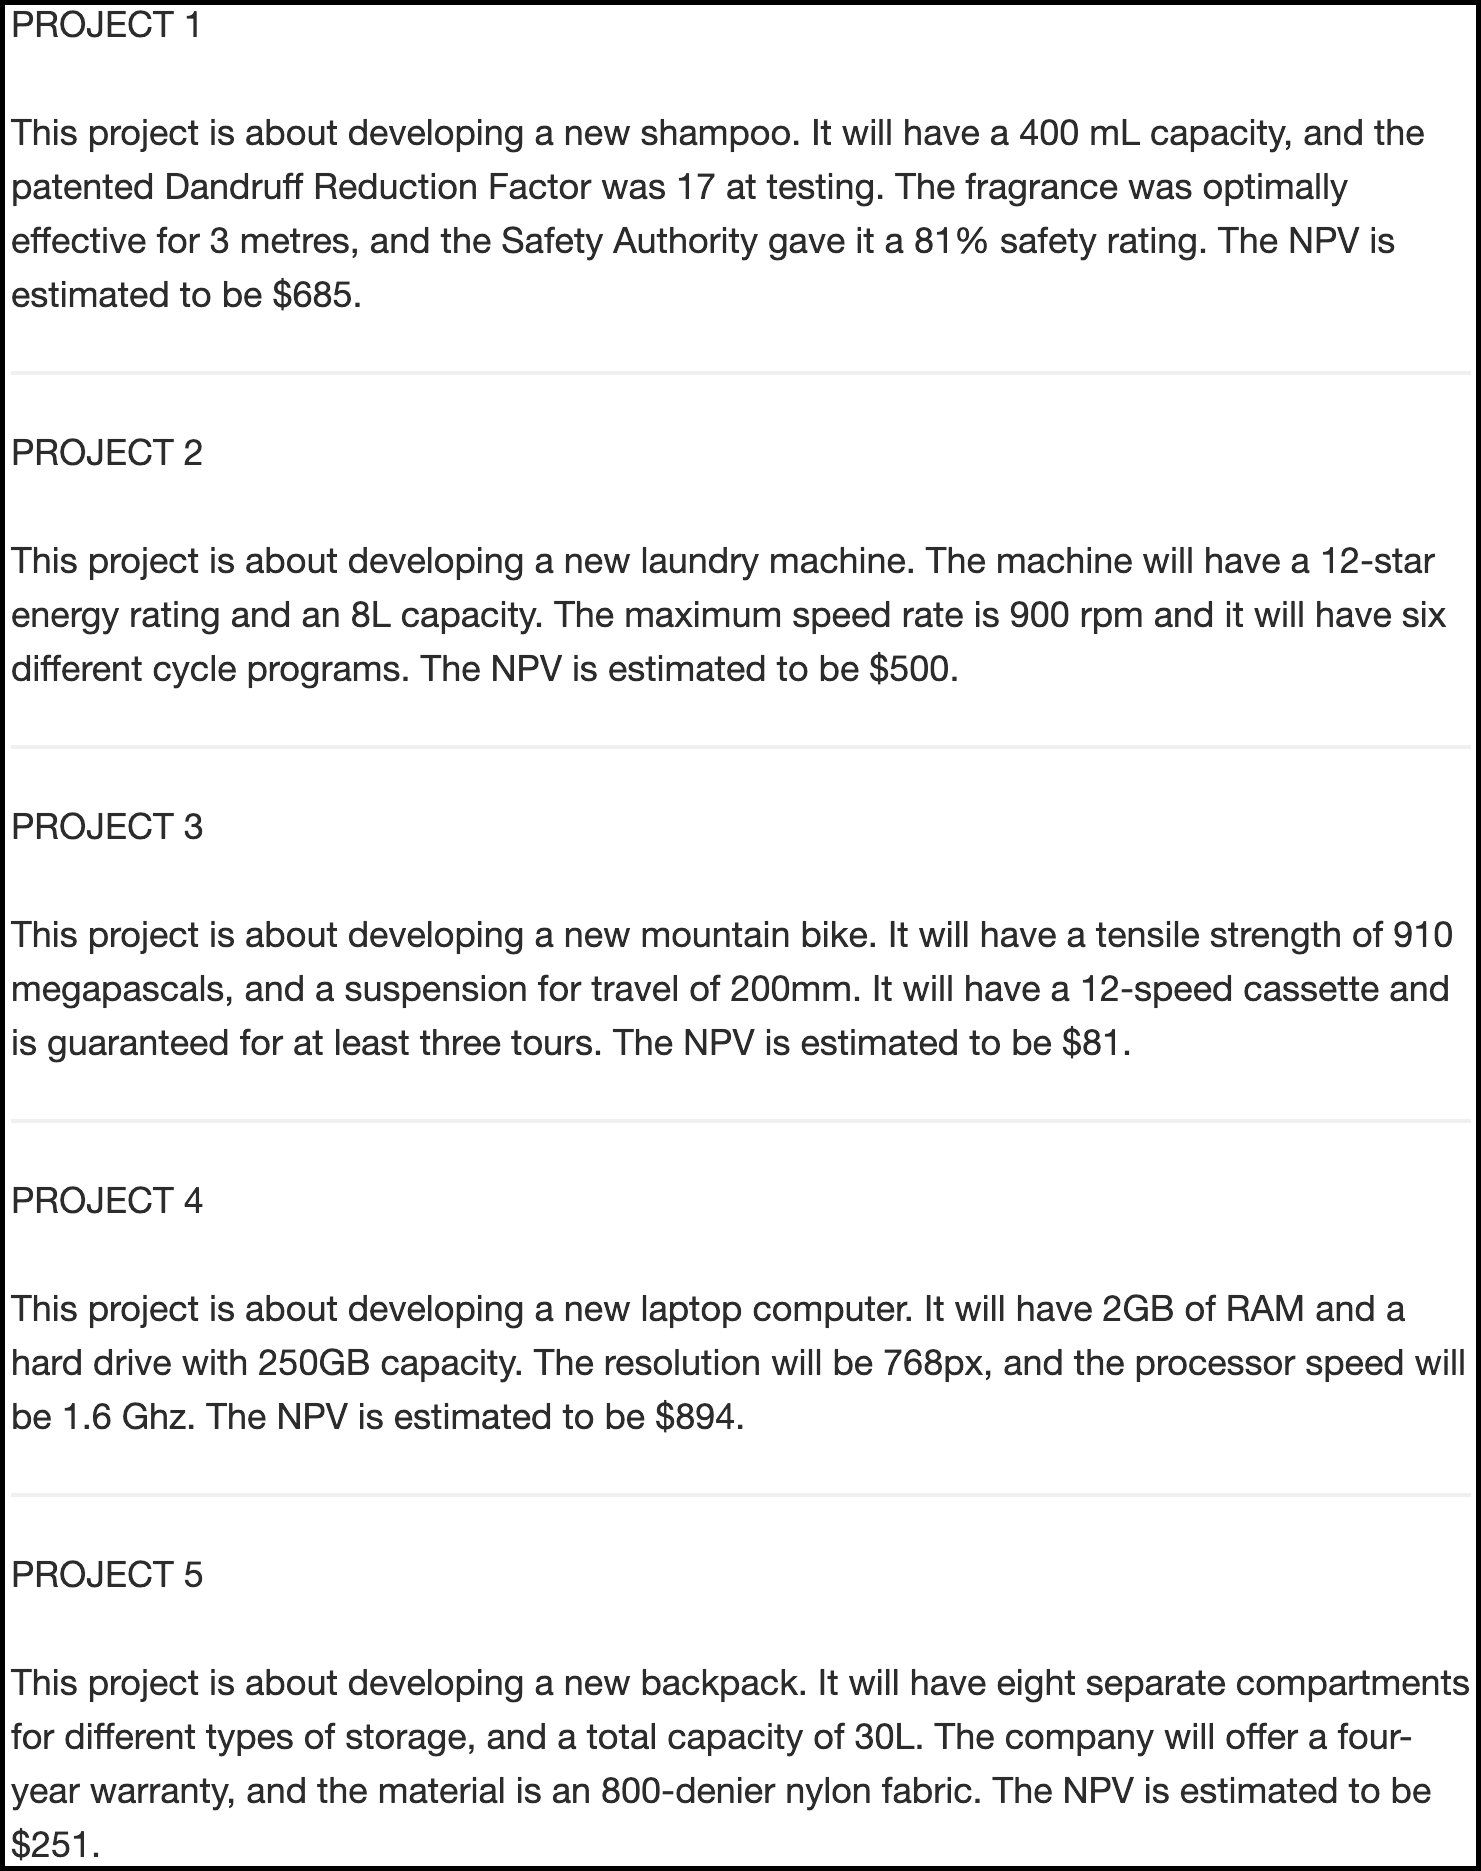
\includegraphics[width=1\linewidth]{thesis_files/figure-latex/projects-alignment-low-materials-alignment-2-1} \caption{An example of a low alignment display in Experiment~1. Border added for clarity.}\label{fig:projects-alignment-low-materials-alignment-2}
\end{figure}

Critically, the value of the concrete attributes were always in conflict with
the NPV. For instance, Project 4 always had the lowest value for each of the
concrete attributes for laptops, but always had the highest NPV. This meant that
participants' allocations could be used as a proxy measure for an individual's
degree of dependence on NPV.

\paragraph{Allocation}

Participants completed a capital allocation task (see
Figure~\ref{fig:allocation-alignment-2}), adapted from \textcite{bardolet2011}, in which
they were asked to allocate a hypothetical yearly budget across the given five
projects.



\begin{figure}
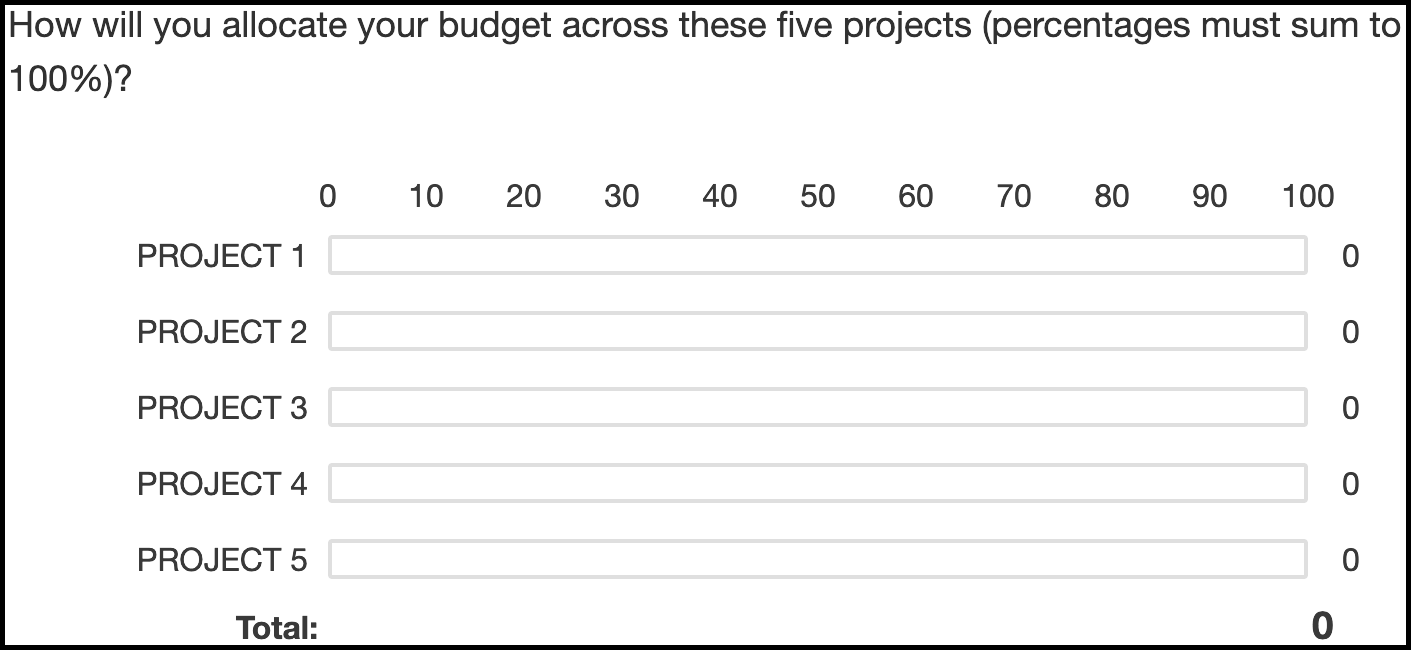
\includegraphics[width=1\linewidth]{thesis_files/figure-latex/allocation-alignment-2-1} \caption{The allocation task. Border added for clarity.}\label{fig:allocation-alignment-2}
\end{figure}

\paragraph{Additional measures}

Other measures were included apart from allocation. The stimuli and analyses for
these measures are reported in Appendices~\ref{materials-alignment-2-appendix}
and~\ref{results-alignment-2-appendix}, respectively. Specifically,
participants were asked to forecast the future returns of the projects (see
Figure~\ref{fig:forecasting-materials-alignment-2}), rank the projects (see
Figure~\ref{fig:ranking-materials-alignment-2}), indicate their confidence in
their decisions (see Figure~\ref{fig:confidence-materials-alignment-2}), and
justify their decisions (see
Figure~\ref{fig:justification-materials-alignment-2}).

\subsubsection{Procedure}

After reading the relevant instruction page, participants completed the
forecasting task directly after each project display in the low alignment
condition. For the high alignment condition this was done directly under all
projects. Participants then ranked the projects and subsequently answered the
allocation, confidence, and justification questions.

\subsection{Results}

A mixed factorial ANOVA was conducted to investigate the effects of alignment
and NPV reliability on participants' allocations. As seen in
Figure~\ref{fig:plot-alignment-2-allocation}, the alignment \(\times\)
reliability amount \(\times\) NPV amount interaction was significant,
\(F(6.57, 367.76) = 2.18\), \(p = .039\), \(\hat{\eta}^2_p = .038\). The
analyses excluding the no NPV condition showed the expected results. The NPV
amount trend was higher in the low alignment condition than in the high
alignment condition, \(M = 61.70\), 95\% CI \([33.02,~90.37]\), \(t(76) = 4.29\), \(p < .001\),
averaging over reliability amount. This shows that people relied on NPV more
when projects were dissimilar than when they were similar.

Further, the NPV amount \(\times\) reliability amount interaction was
stronger in the high alignment condition than in the low alignment condition,
\(M = 67.81\), 95\% CI \([10.47,~125.16]\), \(t(76) = 2.36\), \(p = .021\). Specifically, in
high alignment, the NPV amount trend was higher in the high reliability
condition than in the low reliability condition,
\(M = -63.47\), 95\% CI \([-100.00,~-26.94]\), \(t(112) = -3.44\), \(p = .001\), whereas in low
alignment, there was no significant difference between reliability conditions,
\(M = 4.35\), 95\% CI \([-34.52,~43.21]\), \(t(112) = 0.22\), \(p = .825\). This shows that people
only used the reliability information to moderate their allocations when
projects were similar and not when they were dissimilar.

The comparison with the no NPV condition revealed the expected pattern. In high
alignment, the linear NPV trend was only significantly lower in the no NPV
condition than the high reliability condition,
\(M = 75.70\), 95\% CI \([39.17,~112.24]\), \(t(112) = 4.11\), \(p < .001\), and not the low
reliability condition, \(M = 12.24\), 95\% CI \([-27.94,~52.41]\), \(t(112) = 0.60\), \(p = .547\).
However, in low alignment, the linear NPV trend was significantly lower in the
no NPV condition than both the low reliability condition,
\(M = 64.63\), 95\% CI \([25.76,~103.50]\), \(t(112) = 3.29\), \(p = .001\), and the high
reliability condition, \(M = 60.29\), 95\% CI \([24.14,~96.43]\), \(t(112) = 3.30\), \(p = .001\).



\begin{figure}
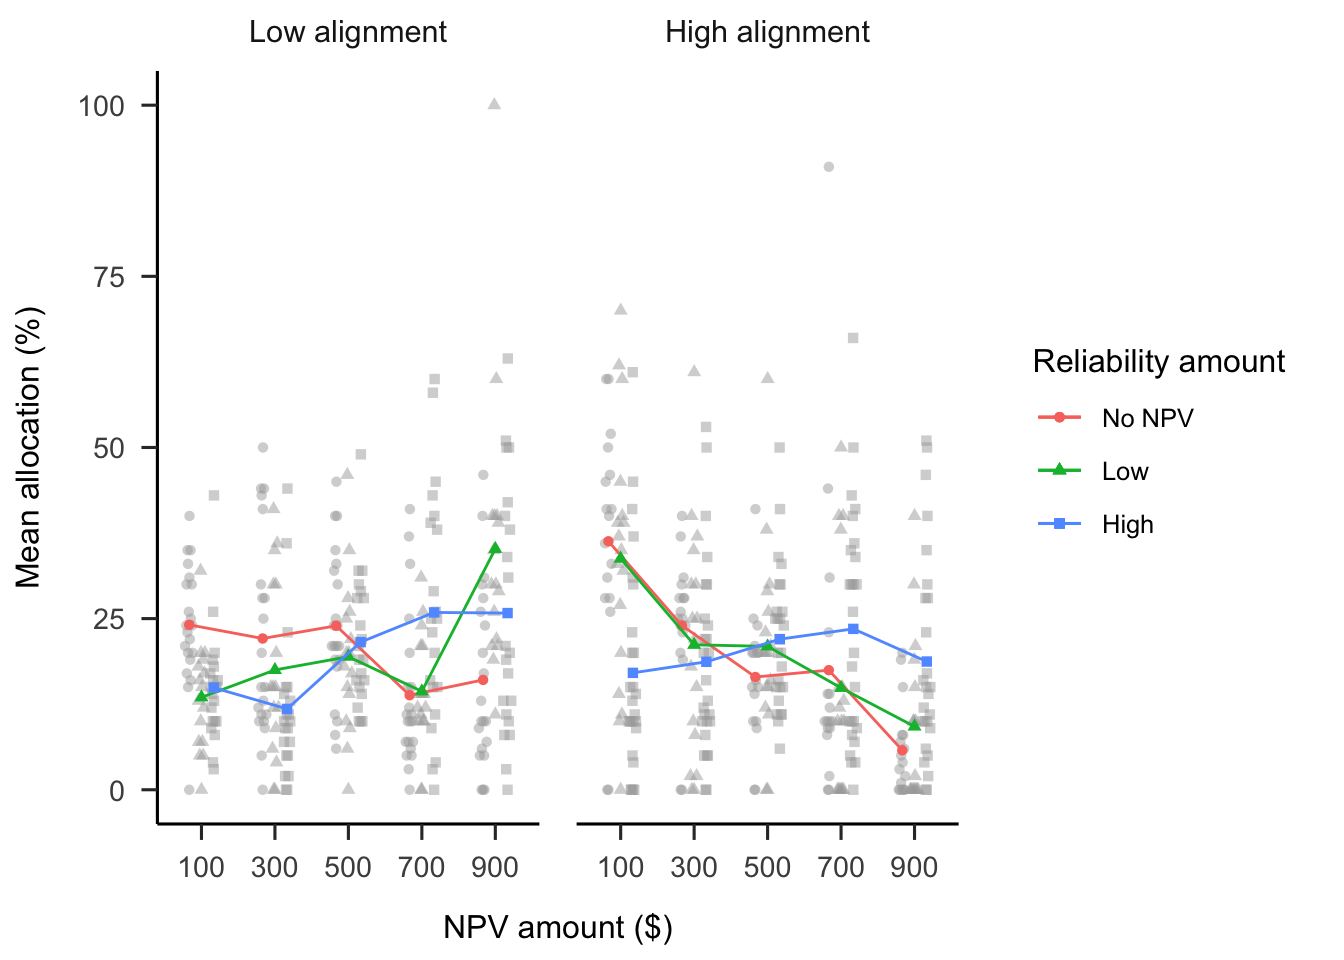
\includegraphics[width=1\linewidth]{thesis_files/figure-latex/plot-alignment-2-allocation-1} \caption{Mean allocation. Error bars represent 95\% confidence intervals based on the multivariate model. Note that this mixed factorial design does not allow for using confidence intervals to make inferences by ``eye'' across conditions.}\label{fig:plot-alignment-2-allocation}
\end{figure}

The ranking, confidence, and forecast mean data were all largely congruent with
the allocation findings (see Appendix~\ref{results-alignment-2-appendix}). The
results also showed that forecasts of those in the low alignment condition had
higher standard deviations than those in the high alignment condition (see
Appendix~\ref{forecast-sd-alignment-2}). However, this did not replicate in
subsequent experiments (see Appendices~\ref{forecast-sd-alignment-4}
and~\ref{forecast-sd-alignment-5}).

\subsection{Discussion}

Experiment~1 found evidence for the effect of alignment on laypeople's
decision-making in capital allocation scenarios. Specifically, when projects
were comparable, people used NPV when they were told that it was reliable, but
not when they were told that it was unreliable. However, they used NPV
regardless of reliability when it was the only shared dimension across products.

Experiment~1 manipulated \emph{verbal} NPV reliability. That is, participants were
explicitly told whether NPV was considered to be a reliable metric or not.
However, in the real-world the reliability of a metric is more commonly
expressed in numerical form, such as a range around an estimate. Experiment~2
attempted to replicate the alignment effects, while manipulating the \emph{numerical}
NPV reliability associated with each project, rather than the verbal reliability
as used in Experiment~1. Further, people with sufficient experience with
financial theory and analysis might be able to successfully draw inferences from
such information. Therefore, Experiment~2 used a sample of Masters of Management
students, instead of the laypeople used in Experiment~1.

\hypertarget{alignment-3}{%
\section{Experiment~2}\label{alignment-3}}

Experiment~2 investigated the effects of alignment and numerically-expressed
variance information on capital allocation decisions. In Experiment~1 the
information about the variance inherent in the NPVs was communicated explicitly
as the conclusion (e.g., ``NPV is unreliable''). In Experiment~2, however, only
the actual variance information itself was communicated without the conclusion
about its reliability. Specifically, participants saw the range of predicted
values (akin to a confidence interval). Therefore, while Experiment~1
manipulated \emph{verbal} reliability, Experiment~2 manipulated \emph{numerical}
reliability. Further, Experiment~2 studied participants with more business
experience than the previously used laypeople samples. This experiment tested
whether the previous findings of an alignment effect will replicate with people
with more business experience. The experiment also tested whether this
population is sensitive to variance in forecasts.

Hypothesis~\ref{hyp:allocation-alignment-alignment-2} was again tested to
investigate the alignment effect in the new sample. However, the other
hypotheses from Experiment~1 were not tested again because Experiment~2
manipulated numerical reliability and did not include a no NPV condition.
Research has shown that people are poor at reasoning with numerical variance
information \autocite{galesic2010,konold1993,vivalt2021,batteux2020}. Therefore,
Experiment~2 tested the following:

\begin{hypothesis}[No effect of numerical reliability]
\protect\hypertarget{hyp:allocation-npv-reliability-alignment-3}{}{\label{hyp:allocation-npv-reliability-alignment-3} \iffalse (No effect of numerical reliability) \fi{} }The NPV amount \(\times\) reliability amount interaction will not be significant
in either alignment condition.
\end{hypothesis}

Experiment~2 also investigated the potential to quickly change participants'
understanding, if they did not initially use numerical reliability for their
allocations. Therefore, participants were presented with a short lecture on the
importance of paying attention variance in financial decision-making. However,
results were inconclusive, so see Appendix~\ref{alignment-3-appendix} for a
more detailed discussion. Further, Experiment~2 investigated whether
participants would have a higher sense of understanding NPV than they really do
\autocite[as in][]{long2018}. These results are also reported in
Appendix~\ref{alignment-3-appendix} as they were not sufficiently relevant to
this chapter.

\hypertarget{method-alignment-2}{%
\subsection{Method}\label{method-alignment-2}}

\subsubsection{Participants}

Fifty-four people (28 female) were recruited from a Masters of Management course at an Australian university. Age information was not recorded.~Both the reliability amount conditions (low and
high) and alignment conditions (low and high) were presented within subjects and
the order of their presentation was counterbalanced.

\subsubsection{Materials}

\paragraph{Instructions}

Participants were shown similar instructions to Experiment~1 (see
Section~\ref{instructions-materials-alignment-2}). However, here they were
given more information about NPV (about the discount rate and initial
investment). The appendix shows the full instructions (see
Figure~\ref{fig:instructions-materials-alignment-3}).

\paragraph{NPV test}

Participants were presented with a short and simple test of their understanding
of NPV (see Appendix~\ref{npv-test-materials-alignment-3}).

\paragraph{Project display}

As seen in Figures~\ref{fig:projects-alignment-low-materials-alignment-3}
and~\ref{fig:projects-alignment-high-materials-alignment-3}, the project
display was as in Experiment~1, except for the addition of another set of
projects that differed in semantic content. That is, the projects were about
different types of products (to allow for a within-subjects manipulation). Along
with the single NPV, participants saw the forecasted ranges of cash flow that
were used to calculate the NPV. In the low numerical reliability condition, the
ranges were \(\pm85\)\% around the mean (e.g., \$150-\$1850 if the forecast mean was
\$1000); whereas in the high numerical reliability condition, the ranges were
\(\pm5\)\% around the mean (e.g., \$950-\$1050 if the forecast mean was \$1000). Wide
ranges should indicate low reliability in the measure, while narrow ranges
should indicate high reliability. Between the four displays, participants were
told to treat each new set of projects as independent to the other sets.



\begin{figure}
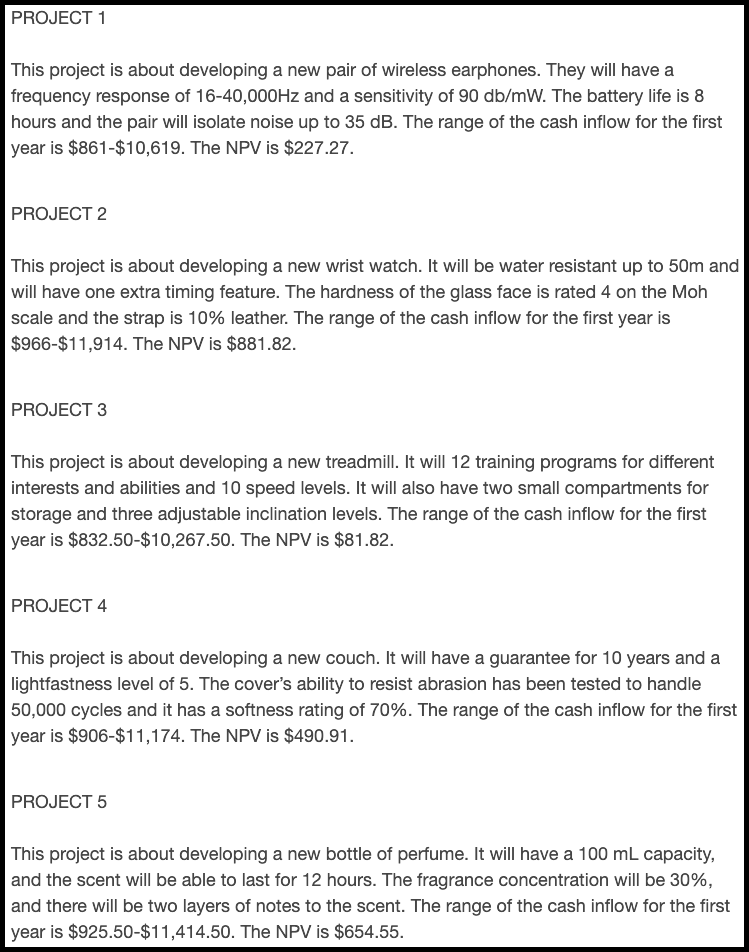
\includegraphics[width=1\linewidth]{thesis_files/figure-latex/projects-alignment-low-materials-alignment-3-1} \caption{An example of a low alignment low reliability display in Experiment~2. Border added for clarity.}\label{fig:projects-alignment-low-materials-alignment-3}
\end{figure}



\begin{figure}
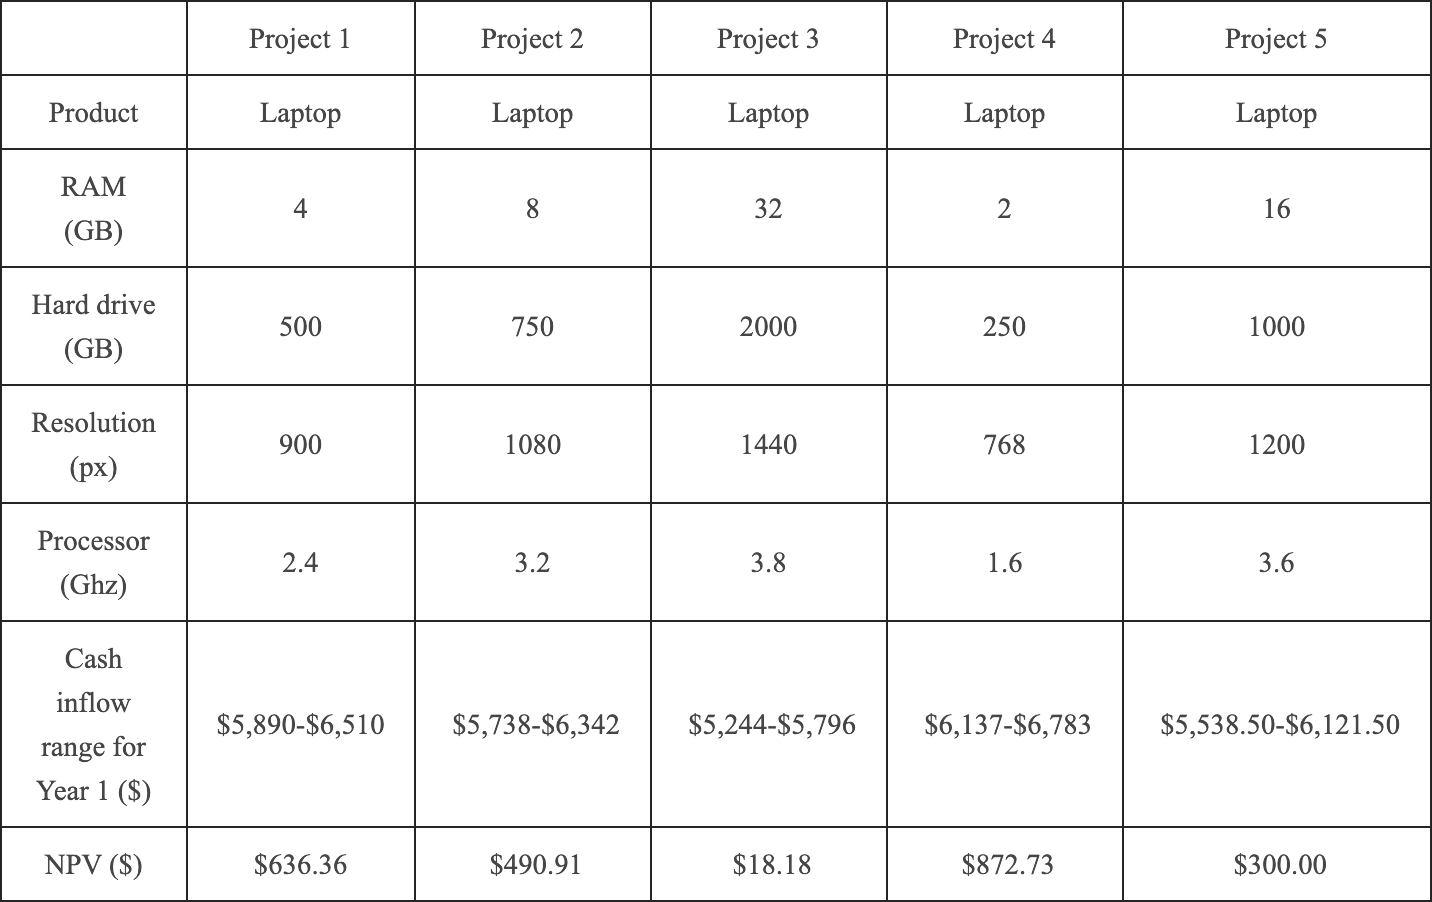
\includegraphics[width=1\linewidth]{thesis_files/figure-latex/projects-alignment-high-materials-alignment-3-1} \caption{An example of a high alignment high reliability display in Experiment~2.}\label{fig:projects-alignment-high-materials-alignment-3}
\end{figure}

\paragraph{NPV knowledge ratings}

Participants were asked to rate the confidence of their knowledge of NPV at
multiple points in the experiment. The appendix shows an example of this display
(see Figure~\ref{fig:npv-knowledge-materials-alignment-3}).

\paragraph{Variance lecture}

Participants were shown a short lecture on the importance of paying attention to
variance information, in an attempt to facilitate a subsequent increased use of
the numerical reliability information in their allocations (see
Appendix~\ref{variance-lecture-materials-alignment-3} for more details and the
lecture slides).

\hypertarget{procedure-alignment-3}{%
\subsubsection{Procedure}\label{procedure-alignment-3}}

Participants saw the instructions and NPV explanation, and completed a simple
test to demonstrate their understanding of NPV. They then completed four
counterbalanced capital allocation trials (equivalent to each condition
combination), and subsequently saw a brief presentation about the importance of
paying attention to variance in financial decision-making. Participants then
completed a further two capital allocation trials of two of the trials that they
saw earlier. They were shown the allocation values that they provided earlier,
and were given the opportunity to change them. Participants rated their
knowledge of NPV once before the NPV test, re-rated after the test, and again
after the four project displays. They were then asked to rate their knowledge of
NPV as they believe it had been both before and after the variance presentation.

\hypertarget{results-alignment-2}{%
\subsection{Results}\label{results-alignment-2}}

A within-subjects factorial ANOVA was conducted to investigate the effects of
NPV amount, alignment, and numerical NPV reliability on participants' project
allocations. Figure~\ref{fig:plot-alignment-3-allocation} shows these data. The
alignment \(\times\) reliability amount \(\times\) NPV amount interaction was
significant,
\(F(2.81, 148.75) = 3.95\), \(p = .011\), \(\hat{\eta}^2_p = .069\).
However, this appeared to be driven by the difference between alignment
conditions in the interaction between the quadratic NPV amount trend and
reliability amount,
\(\Delta M = -42.28\), 95\% CI \([-76.96,~-7.59]\), \(t(53) = -3.14\), \(p = .011\), even after
applying a Šidák correction. The same interaction but with the linear NPV trend
was not significant,
\(\Delta M = -6.13\), 95\% CI \([-31.50,~19.25]\), \(t(53) = -0.62\), \(p = .954\). Further, the linear
NPV trend did not differ between reliability amount condition in neither the low
alignment condition, \(\Delta M = -3.19\), 95\% CI \([-18.77,~12.40]\), \(t(53) = -0.41\), \(p = .683\), nor
the high alignment condition,
\(\Delta M = 2.94\), 95\% CI \([-12.63,~18.52]\), \(t(53) = 0.38\), \(p = .706\). However, averaging over
reliability amount, the linear NPV trend was higher in the low alignment
condition than in the high alignment condition,
\(\Delta M = 28.19\), 95\% CI \([5.57,~50.81]\), \(t(53) = 2.50\), \(p = .016\). This suggests that
participants relied more on NPV when projects were dissimilar than when they
were similar.



\begin{figure}
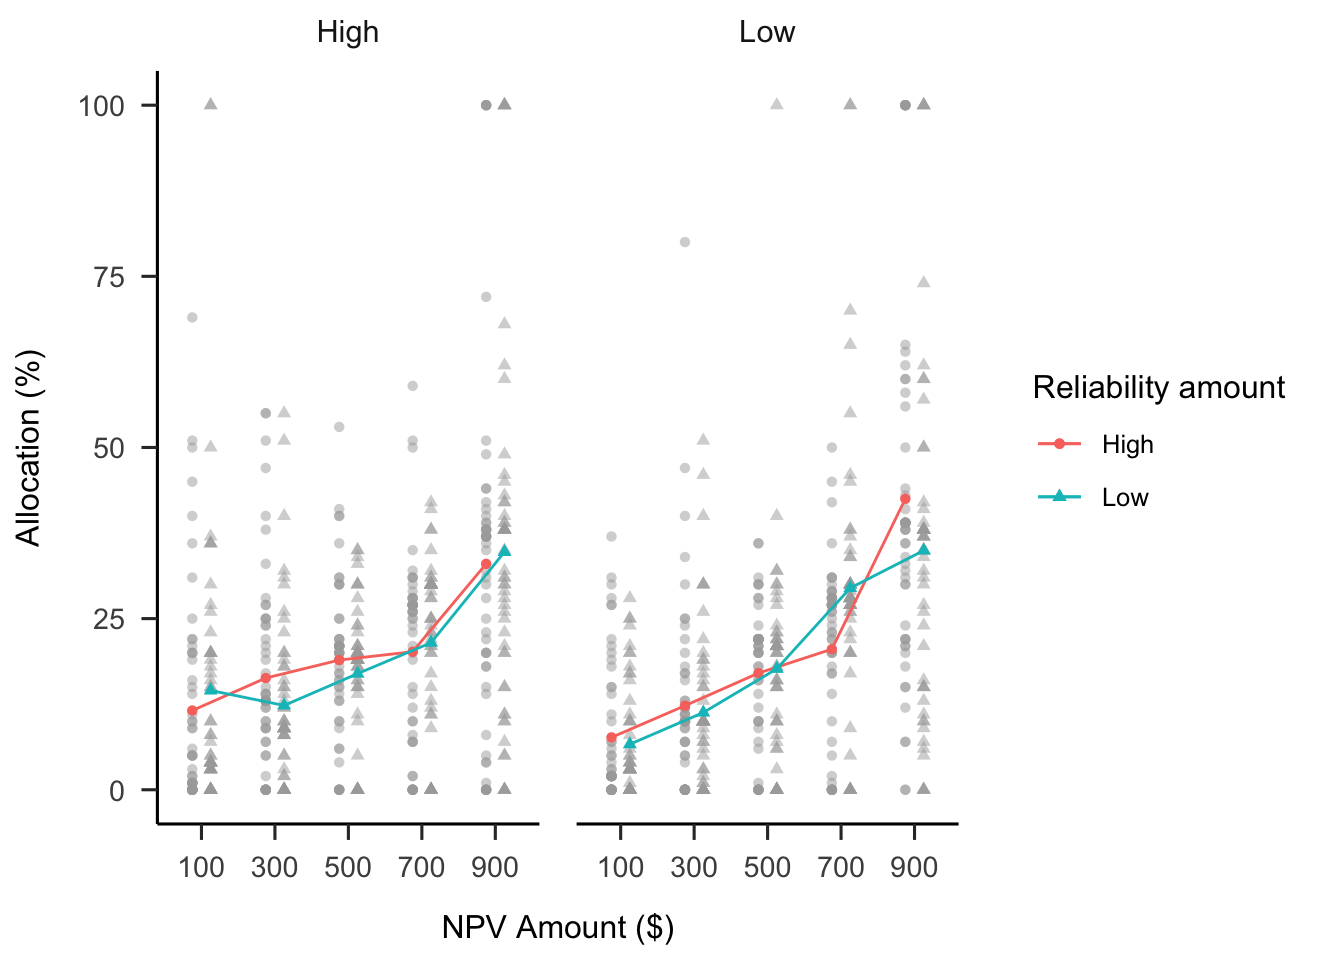
\includegraphics[width=1\linewidth]{thesis_files/figure-latex/plot-alignment-3-allocation-1} \caption{Mean allocation. Error bars represent 95\% confidence intervals based on the multivariate model.}\label{fig:plot-alignment-3-allocation}
\end{figure}

The ranking data were congruent with these results, while the confidence data
were less so. Further, the NPV knowledge data did not replicate the effect from
\textcite[Study 1]{long2018}. These analyses are reported in
Appendix~\ref{results-alignment-3-appendix}.

\subsection{Discussion}

Experiment~2 replicated the alignment effect found in Experiment~1 with
participants with real-world business experience. That is,
Hypothesis~\ref{hyp:allocation-alignment-alignment-2} was supported, as people
relied more on NPV when faced with a set of dissimilar project than when
projects were all from the same domain. Experiment~2 also found evidence for
Hypothesis~\ref{hyp:allocation-npv-reliability-alignment-3}, with no
significant differences between the numerical reliability amount conditions.
While Experiment~2 did not replicate the interaction found in Experiment~1, it
should be emphasised that these are two different effects. In Experiment~1,
participants were explicitly told about the reliability of the NPV measure,
whereas in Experiment~2, they were provided with variance information that
merely implies NPV reliability. Thus, Experiment~2 showed that business students
are affected by comparability of project sets, but not by numerical NPV
reliability information. Specifically, participants appeared to only focus on
the NPV itself, and not on any variations in the underlying noisiness of the
measure for a specific project.

However, it is unclear whether laypeople would also display this variance
neglect. Further, in Experiments~1 and~2, the business projects consisted of a
limited number of domains. It is unclear to what extent these specific domains
influenced the results. These projects were centred around consumer products,
which were originally chosen to be more easily accessible to participants
without business experience. However, with these projects, individual features
do not necessarily indicate a project's profitability. For instance, a laptop
with a low capacity can be more profitable than a laptop with a high capacity
due to the existence of consumer goods markets. Experiment~3 addressed these
limitations.

Another limitation of the last two experiments was the potential presentation
style confound. The two alignment conditions differed in the number of alignable
differences, but also in the way that the information was presented. The
information in the low alignment condition was presented in paragraphs, whereas
the information in the high alignment condition was presented in tables. While
it is likely that each of these data types would be presented in this way in a
business setting, it is important to rule out that this manipulation did not
also unnecessarily increase task difficulty. Therefore, Experiment~3 attempted
to replicate this effect, while controlling for presentation style.

\hypertarget{alignment-8}{%
\section{Experiment~3}\label{alignment-8}}

Experiment~3 investigated the effects of alignment, reliability type, NPV
amount, and reliability amount on allocations. Experiment~1 manipulated
reliability amount by using \emph{verbal} prompts. That is, participants were told
explicitly whether or not NPV was reliable for a certain project industry.
Experiment~2 investigated whether people were able to extract this same kind of
reliability information from \emph{numerical} prompts. That is, participants saw NPVs
with either wide or narrow ranges, indicating either low or high reliability of
the metric, respectively. However, Experiment~1 sampled laypeople, whereas
Experiment~2 sampled a Masters of Management course. Therefore, it was not
possible to compare the two reliability types (verbal and numerical) without
ruling out the potential confound of population type. As such, Experiment~3
manipulated NPV amount, alignment, and reliability amount, but also added a
reliability type factor. Further, presentation style was a possible confound in
the alignment manipulation of the previous experiments. That is, the business
projects in the high alignment condition were always displayed as a part of a
table, whereas the projects in the low alignment condition were displayed in
prose, as paragraphs. Experiment~3 fixed this by using the same presentation
style across alignment condition.

The expected pattern of results in the verbal reliability condition of
Experiment~3 was a replication of Experiment~1. For the numerical reliability
condition, findings from a pilot experiment (detailed in
Appendix~\ref{alignment-7}) were used for predictions. This experiment found no
significant differences in a similar numerical reliability condition to the one
used in Experiment~3. This was therefore expected also for the present numerical
reliability condition. The appendix shows a simulation of these hypothesised
effects (see Figure~\ref{fig:plot-simulation-alignment-8}). Therefore, as well
as again testing
Hypotheses~\ref{hyp:three-way-alignment-2},~\ref{hyp:allocation-alignment-alignment-2},~\ref{hyp:allocation-alignment-reliability-npv-alignment-2},~\ref{hyp:allocation-alignment-high-alignment-2},
and~\ref{hyp:allocation-alignment-low-alignment-2} for the verbal reliability
condition, Experiment~3 tested the following:

\begin{hypothesis}[Overall effect]
\protect\hypertarget{hyp:four-way-alignment-8}{}{\label{hyp:four-way-alignment-8} \iffalse (Overall effect) \fi{} }The alignment \(\times\) reliability amount \(\times\) reliability type \(\times\) NPV
amount interaction will be significant, such that the effects hypothesised above
will be seen in the verbal reliability condition, but none of these effects
will be seen in the numerical reliability condition.
\end{hypothesis}

\subsection{Method}

\subsubsection{Participants}

Four hundred and forty-eight people (176 female) were recruited from the online recruitment platform Prolific. Participants were compensated at a rate of £5 an hour. The average age was 41.65 (\emph{SD} = 10.3, \emph{min} = 29, \emph{max} = 78). Participants reported an average of 6.94 (\emph{SD} = 8.23, \emph{min} = 0, \emph{max} = 43) years of work in a business setting, and an average of 3.73 (\emph{SD} = 6.27, \emph{min} = 0, \emph{max} = 45) years of business education. The mean completion time was 11.35 (\emph{SD} = 10.79, \emph{min} = 1.92, \emph{max} = 183.7) minutes.~Table~\ref{tab:condition-allocation-alignment-8}
shows the between-subjects condition allocation. The two reliability amount
conditions (low and high) were presented within subjects and the order of their
presentation was randomised. As before, NPV amount was varied within subjects.
Therefore, each participant saw two separate project displays.
Appendix~\ref{power-analysis-alignment-8} describes the power analysis
conducted to arrive at the sample size.

\begin{table}[tbp]

\begin{center}
\begin{threeparttable}

\caption{\label{tab:condition-allocation-alignment-8}Experiment 3 group allocation.}

\begin{tabular}{lll}
\toprule
Alignment & \multicolumn{1}{c}{Reliability type} & \multicolumn{1}{c}{N}\\
\midrule
High & Explicit & 112\\
High & Implicit & 112\\
Low & Explicit & 112\\
Low & Implicit & 112\\
Total & - & 448\\
\bottomrule
\end{tabular}

\end{threeparttable}
\end{center}

\end{table}

\subsubsection{Materials}

\paragraph{Instructions}

Participants saw similar instructions to the previous experiments, with an added
explanation of the NPV reliability information for each reliability type
condition (see Appendix~\ref{instructions-materials-alignment-8-appendix}).
Further, they completed a test of basic NPV understanding. This test functioned
also as an attention check as, although it was required to answer, the response
should only be one of two letters.

\paragraph{Project display}

The project displays were similar to the previous experiments. Here, however,
participants saw the same presentation style in both alignment conditions. Each
display had a table describing the projects in the set, with ranking and
allocation inputs. The project details were presented as dot points within the
relevant cells of the table.
Figure~\ref{fig:projects-alignment-low-reliability-explicit-low-materials-alignment-8}
shows an example of a low alignment, low verbal reliability display; and
Figure~\ref{fig:projects-alignment-high-reliability-implicit-high-materials-alignment-8}
shows an example of a high alignment, high numerical reliability display.



\begin{figure}
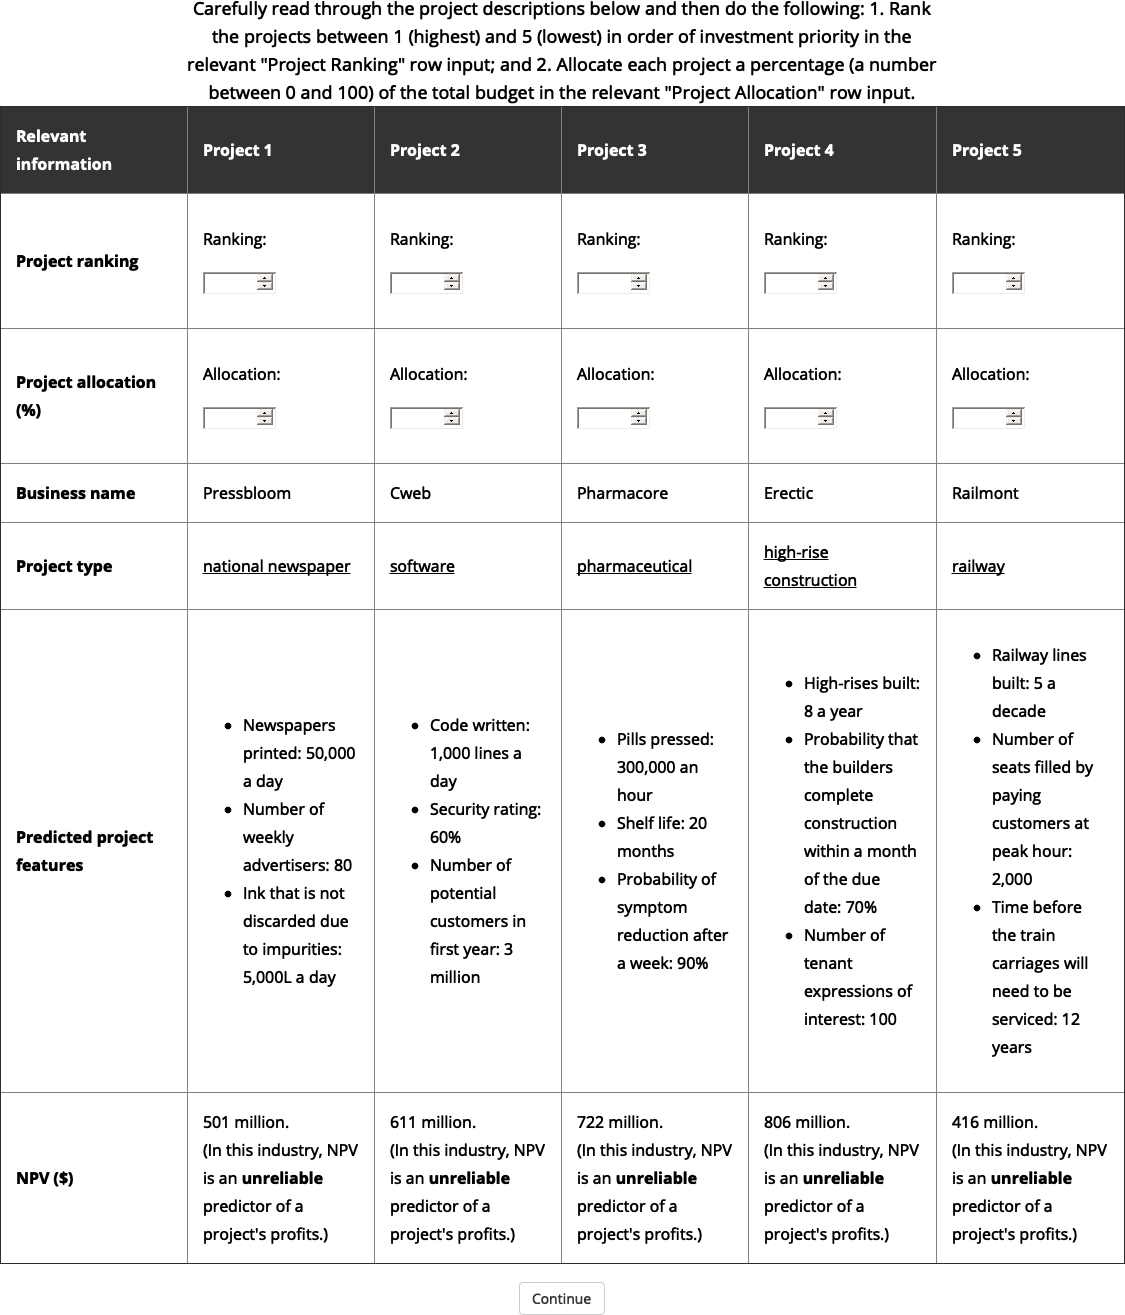
\includegraphics[width=1\linewidth]{thesis_files/figure-latex/projects-alignment-low-reliability-explicit-low-materials-alignment-8-1} \caption{An example of a low alignment, low verbal reliability display in Experiment~3.}\label{fig:projects-alignment-low-reliability-explicit-low-materials-alignment-8}
\end{figure}



\begin{figure}
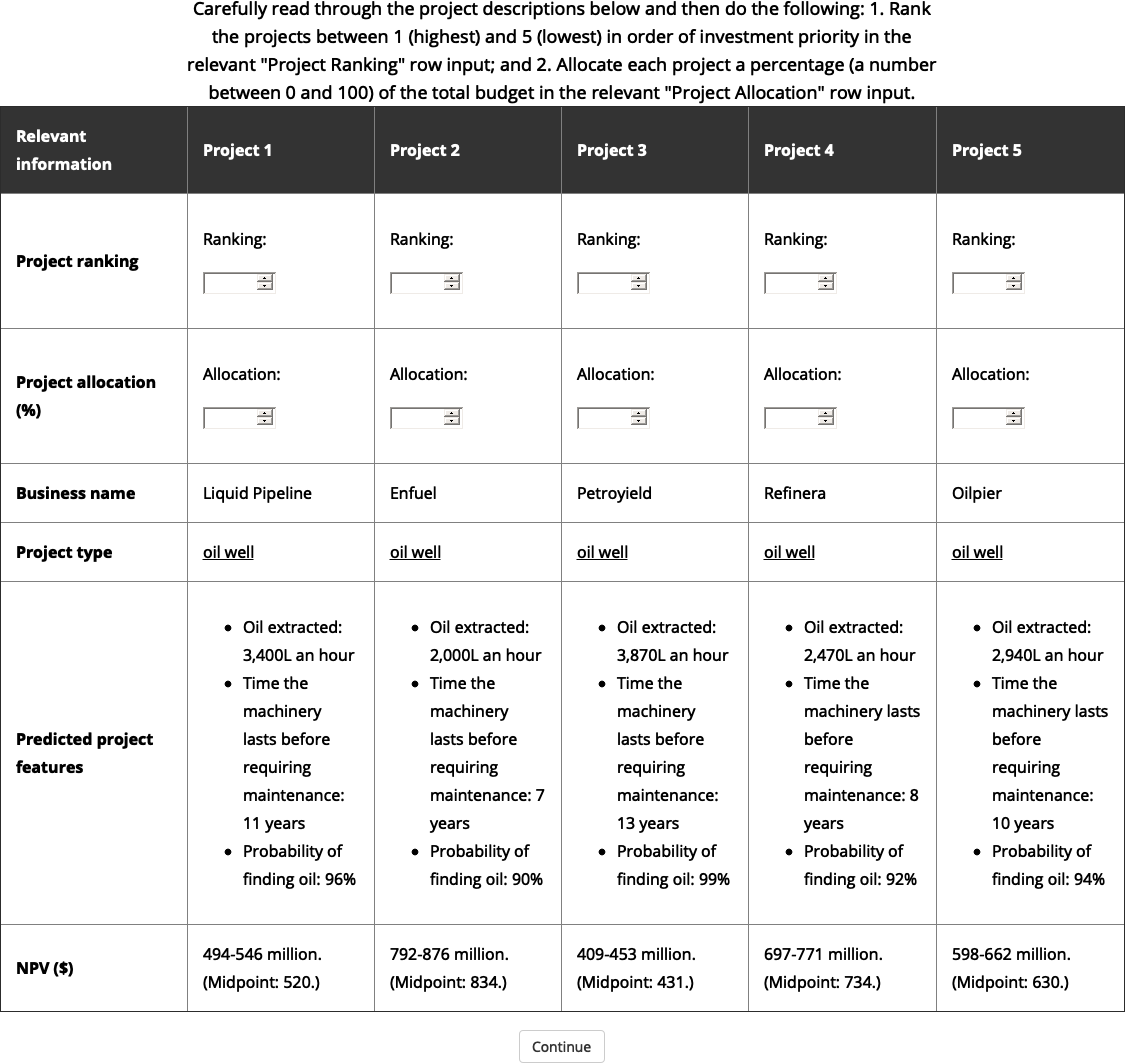
\includegraphics[width=1\linewidth]{thesis_files/figure-latex/projects-alignment-high-reliability-implicit-high-materials-alignment-8-1} \caption{An example of a high alignment, high numerical reliability display in Experiment3.}\label{fig:projects-alignment-high-reliability-implicit-high-materials-alignment-8}
\end{figure}

Three elements were counterbalanced: 1. the association of reliability amount
and project set (two variations), 2. the association of business name with NPV
(five latin square variations), and 3. project variation (five variations per
alignment condition). For high alignment, project variation meant the project
type. For low alignment, this meant the intrinsic feature variant for the
relevant project type. Table column order and project display order were both
randomised.

\paragraph{Interstitial}

Before each project display, participants saw an ``interstitial'' page, whose role
was to 1. introduce the next display, and 2. check the participant's attention
(not required to answer, so can be skipped if the interstitial text isn't read).
See Figure~\ref{fig:interstitial-materials-alignment-8} in the appendix for an
example.

\subsection{Results}

A mixed factorial ANOVA was conducted to investigate the effects of NPV amount,
alignment, NPV reliability amount, and NPV reliability type on participants'
project allocations. Figure~\ref{fig:plot-alignment-8-allocation} shows these
data. Only the main results are reported here, while the rest of the
hypothesised allocation effects are reported in
Appendix~\ref{results-alignment-8-allocation}. The predicted four-way
interaction (alignment \(\times\) reliability amount \(\times\) NPV amount \(\times\)
reliability type) was not significant,
\(F(3.20, 1,420.19) = 0.71\), \(p = .555\), \(\hat{\eta}^2_p = .002\). However, most of the
hypothesised specific effects were found.

\subsubsection{Verbal reliability}

The three-way interaction (alignment \(\times\) reliability amount \(\times\) NPV
amount) in the verbal reliability condition was not significant,
\(\Delta M = 13.42\), 95\% CI \([-1.27,~28.11]\), \(t(444) = 1.80\), \(p = .073\). This is
most likely due to the size of the two-way interactions in each alignment
condition being relatively similar, despite the expectation of no interaction in
the low alignment condition (as was seen in Experiment~1). In high alignment,
the interaction between the linear NPV amount trend and NPV reliability amount
was significant,
\(\Delta M = -36.63\), 95\% CI \([-47.02,~-26.25]\), \(t(444) = -6.93\), \(p < .001\).
Specifically, the trend was stronger in the high reliability amount condition,
\(\Delta M = 27.26\), 95\% CI \([17.69,~36.83]\), \(t(444) = 5.60\), \(p < .001\),
than in the low reliability amount condition,
\(\Delta M = -9.38\), 95\% CI \([-18.86,~0.11]\), \(t(444) = -1.94\), \(p = .053\).
This shows that, as in Experiment~1, participants moderate their allocations
based on verbally-expressed NPV reliability.

Contrary to Experiment~1, the interaction between the linear NPV amount trend
and NPV reliability amount was significant in low alignment,
\(\Delta M = -23.21\), 95\% CI \([-33.60,~-12.83]\), \(t(444) = -4.39\), \(p < .001\).
This suggests that participants were also able to moderate their allocations
based on verbal reliability in the low alignment condition. Despite the lack of
a three-way interaction in the verbal reliability condition (that would have
indicated a difference in the two alignment two-way interactions), the linear
NPV amount trend was stronger in the low alignment condition than in the high
alignment condition when averaging over reliability amount,
\(\Delta M = 28.97\), 95\% CI \([17.68,~40.26]\), \(t(444) = 5.04\), \(p < .001\). This
suggests that when NPV reliability was expressed verbally, as in Experiment~1,
participants relied more on NPV when projects were dissimilar than when they
were similar.

\subsubsection{Numerical reliability}

In the numerical reliability condition, the linear NPV amount trend was not
significantly ``equivalent'' between those in the low and high alignment
conditions (averaging over reliability amount),
\(\Delta M = 15.19\), 95\% CI \([3.90,~26.48]\), \(t(444) = 2.64\), \(p = .996\). In
fact, a post-hoc comparison suggests that the low alignment trend was stronger
(with Bonferroni adjustment),
\(\Delta M = 15.19\), 95\% CI \([0.78,~29.60]\), \(t(444) = 2.64\), \(p = .034\). This is
the same pattern as in the verbal reliability condition above and in
Experiment~2. Further, the linear NPV trend was not significantly different
between reliability amount conditions in both the low alignment condition,
\(\Delta M = 1.64\), 95\% CI \([-11.61,~14.90]\), \(t(444) = 0.31\), \(p > .999\),
and high alignment condition,
\(\Delta M = -1.21\), 95\% CI \([-14.46,~12.05]\), \(t(444) = -0.23\), \(p > .999\).
This shows that participants did not use numerical reliability to moderate their
allocations.



\begin{figure}
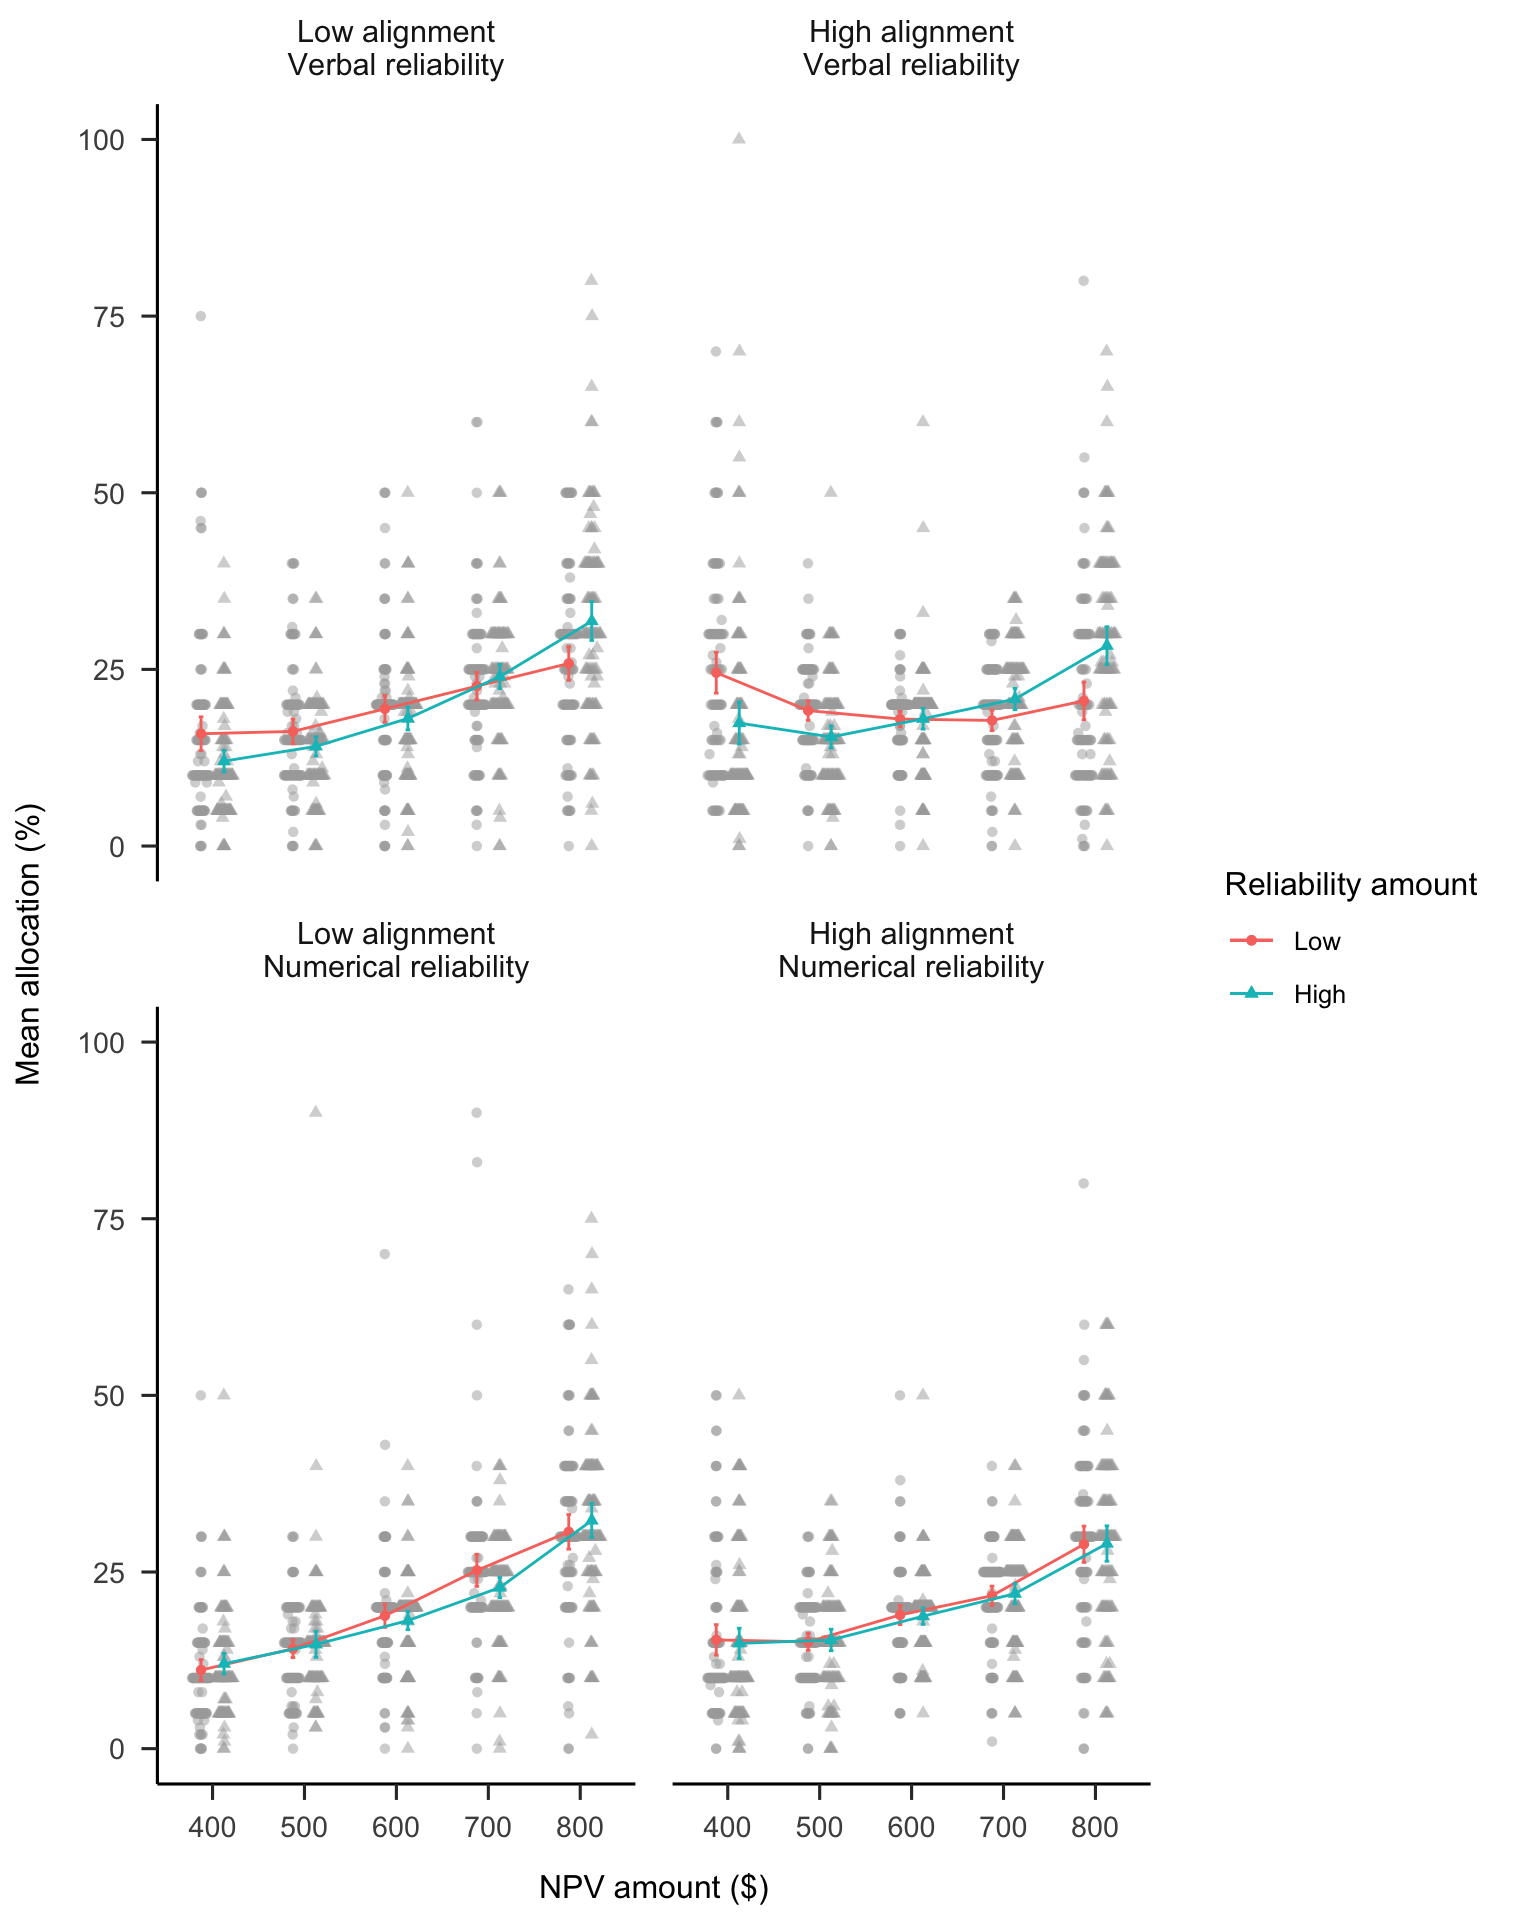
\includegraphics[width=1\linewidth]{thesis_files/figure-latex/plot-alignment-8-allocation-1} \caption{Mean project allocation for all conditions. Error bars represent 95\% confidence intervals based on the multivariate model. Here, however, the intervals are so narrow that they are mostly obscured by the mean indicators in the plot.}\label{fig:plot-alignment-8-allocation}
\end{figure}

\subsection{Discussion}

Hypotheses~\ref{hyp:three-way-alignment-2},~\ref{hyp:allocation-alignment-alignment-2},~\ref{hyp:allocation-alignment-reliability-npv-alignment-2},
and~\ref{hyp:allocation-alignment-high-alignment-2} were supported in the
verbal reliability condition. This shows that, while overall participants prefer
to use NPV as a proxy for project quality in their allocations, they still use
verbal reliability information. Specifically, when projects are similar, people
use NPV when they are told that it is reliable, and use alternative metrics when
told that it is not reliable. However, Experiment~3 did not find evidence for
Hypothesis~\ref{hyp:allocation-alignment-low-alignment-2}. Instead,
Experiment~3 found that even in the low alignment condition, participants still
moderated their use of NPV. They still used NPV regardless of reliability
condition, shown by the positive NPV amount trend in both reliability
conditions. However, Experiment~3 shows that participants used NPV less when
told that it was unreliable.

Further, Experiment~3 did not find support for
Hypothesis~\ref{hyp:four-way-alignment-8} mostly likely because of the
unexpected effects of NPV amount in the numerical reliability condition. The
hypothesis was constructed in response to the results of a pilot study
(documented in Appendix~\ref{alignment-7}) that replicated the results of
Experiment~1 in the verbal reliability condition, but did not replicate the
results of Experiment~2 in the numerical reliability condition. That is, when
faced with numerical ranges as variance information, people did not seem to even
use the midpoint in their decisions. Experiment~3, on the other hand, replicated
the finding of Experiment~2 in the numerical reliability condition.
Specifically, people used NPV more when projects were dissimilar, but
critically, they did not use numerical range information to moderate their
allocations.

\section{General discussion}

Across three experiments there were two main findings: 1. NPV is used more when
options are hard to compare; and 2. people do not consider numerical variance
information, despite this being important to the reliability of the NPV
forecasts. These effects were consistent across both naive and experienced
populations, which indicates their persistence. People make use of metrics with
alignable differences when in a situation that requires comparison across
disparate options. However, they do not sufficiently moderate their use of such
metrics even when they have alternative attributes to use.

Experiment~1 found that when participants were told that NPV was unreliable,
they did not use it in their allocation decisions, but when they were told that
it was reliable they did. Experiment~2 found that people with some business
experience relied on NPV more for capital allocation when the rest of the
information was non-alignable, compared to when it was alignable. However,
participants did not take into account the numerical reliability information
when making these decisions. Experiment~3 found further evidence of these
effects, within one experimental design.

Alignable differences have been shown to be important to decision making in many
settings \autocite{markman2010,markman1995}. The experiments in this chapter are novel
in the investigation of alignment effects in a capital allocation paradigm.
Further, these experiments considered the extent to which the reliability of an
alignable measure (NPV) affects the way people use it. The experiments found
that this is dependent on the availability of other alignable differences in the
choice set. If other alignable differences are available, then participants are
willing to reduce their use of a supposedly unreliable alignable measure (and
use it when told that it is reliable). However, when no other alignable
differences are available, then the unreliable, but alignable, measure is used
less. This was found in both Experiment~1 and~3, as well as to lesser extent in
a pilot study (reported in Appendix~\ref{alignment-1}).

Financial measures such as NPV are useful because of their alignability. That
is, they act as an alignable difference regardless of the inherent similarity of
a set of projects. Psychologically, these measures are useful because they allow
for relevant inferences \autocite{lassaline1996} and because they offer an abstraction
of concrete details \autocite{doumas2013}. However, the theoretical account of
structural alignment does not directly speak to the real-world implications when
there is a need for non-alignable comparisons. NPV is a type of abstraction that
allows comparison between different aspects of a company. For instance,
comparing an oil field project with a refinery project might be made easier by
using NPV. On the other hand, this increased alignment might actually hide
important information because it does not consider the finer complexities
inherent within each business unit. The forecasts use to calculate NPV are based
on different indicators in each business unit, and there are likely to be
differences in variance between each unit's estimates. As such, one can imagine
a continuum of similarity comparisons in which usefulness of comparison
increases with the level of alignability, but is moderated by the level of
abstraction that is required to achieve the alignment.

The finding that people, even with some business experience, do not sufficiently
consider variance information is surprising, but understandable. It is
surprising because so much of financial decision making depends on considering
different sources of variance (e.g., risk, volatility, and uncertainty).
However, it is understandable because research from psychology and statistics
education shows that statistics students and people in general have a poor
ability to draw statistical inferences \autocites[e.g.,][]{galesic2010,konold1993}. Future
research should investigate the conditions under which people's sensitivity to
variance information can be facilitated. For instance, it is unclear whether it
is merely salience that is lacking, and that therefore visual aids could be
useful, or whether further explicit explanation of the statistical inference is
necessary. Pilot experiments suggest that participants still struggle to use
numerical reliability information, even when given very explicit instructions
(see Appendix~\ref{alignment-6}).

A possible limitation of these experiments is the use of NPV as the only
financial metric. In the business world there are many metrics that serve
similar functions and would be used as a tool to deal with non-alignable
options, as NPV was in the current study. Therefore, future research should
attempt to replicate the current findings with different financial measures.

Future research should also investigate the boundary conditions of the
reliability effect. That is, people seem to be responding to explicit
reliability information, but not to variance information that implies
reliability. Future research should attempt to identify the minimal kind of
information about variance that participants need in order to understand the
relevant implications about reliability. Participants may simply not notice the
variability information, or assume that it irrelevant. For instance, future
research could test participants in a condition in which the variability
information is more salient.

\newpage

\printbibliography[segment=\therefsegment,heading=subbibintoc]

\hypertarget{interstitial-2}{%
\chapter{Looking for alignment in past cases}\label{interstitial-2}}

Chapter~\ref{alignment} found that people do not sufficiently weigh the
importance of numerical variance information in capital allocation. This is
important for when projects are dissimilar because people might not pay
attention to the variance that underlies NPV. However, there are also
implications for high alignment scenarios. When projects are alignable this
means that managers are likely to have a choice of using both abstract metrics
as well as intrinsic project features. Managers may use a metric such as NPV,
whose variance may suggest a lack of reliability, despite being able to use
intrinsic projects features. They may therefore miss out on an opportunity to
use different, potentially more reliable measures.

An evaluation of a non-alignable set of projects can therefore lead to many
potential pitfalls. Such a situation is likely to occur in most hierarchical
organisations and be more common the more the organisation is diversified.
Chapter~\ref{interstitial-1} discussed that a solution to managers not
aggregating the risk of multiple projects is a concurrent evaluation of projects
as a portfolio. However, the solution to the evaluation of dissimilar project in
the case of a diversified organisation is likely to involve significantly more
difficult structural changes in the organisation. For instance, this may mean
divesting certain divisions of the organisation, as GE has been doing over the
last few years \autocite{scott2018}.

Other solutions are also possible. For instance, organisations can develop a
more normative use of metrics and take into account underlying uncertainty.
However, this kind of change might require substantially more statistical
reasoning abilities than can be expected of managers without better decision
guidelines. Another solution managers may use is to look to evidence from
similar projects from outside the organisation. This is useful because a
diversified organisation may not have enough points of reference for a project
proposal within it. Doing this both does not require substantial restructuring
of the organisation as in divestment and is already an on-going practice, as
opposed to aiming to facilitate managers' statistical reasoning.

Evidence from similar projects may come in the form of an individual case study
from another organisation, or a research report that describes a statistical
result. Case studies are especially important in managerial decision-making
since they are used extensively in business school teaching materials.
Therefore, managers are likely to look to case studies to inform their
decisions. But would they think that a single case study is more useful than
statistical data? The literature on anecdotal bias suggests that they might.
Therefore, Chapter~\ref{anecdotes} considers the influence of an anecdote on
project allocation when it conflicts with statistical evidence.

Previous work showed that people often do not give evidence appropriate
weighting in their decisions \autocite{griffin1992}. Anecdotal and statistical evidence
are potentially conflicting sources of evidence, so it is important to
appropriately weigh their influence when making a decision. It is possible for
these sources of evidence to conflict because statistical estimates commonly
refer to the mean value of a distribution, whereas individual cases may be
sampled, for instance, from either tail of the distribution. This kind of
comparison would give the appearance of conflicting information, especially if
the distribution is skewed. In the same way that in Chapter~\ref{alignment} the
intrinsic project features conflicted with the abstract financial metric, in
Chapter~\ref{anecdotes} the description of an anecdote conflicted with the
financial metrics of the target project.

Chapter~\ref{anecdotes} considered how people dealt with such conflicting
information. That is, would they focus on one metric or use a trade-off? In the
previous chapter, people did not seem to predominantly use one cue or another.
The fact that those in the low alignment condition relied on NPV more than those
in the high alignment condition means that those in the high alignment condition
were still referring to the intrinsic project features to some extent.
Specifically, the different measures' influence may have been integrated in a
form of trade-off. However, there was no clear way of determining this, because
the allocation measure was aggregated in the analysis. Chapter~\ref{anecdotes},
however, set up the conditions so that it was possible to determine whether
participants were using anecdotes exclusively, partially, or not at all.



\begin{savequote}
We like stories, we like to summarize, and we like to simplify
\qauthor{---Nassim Nicholas \textcite[p.~63]{taleb2007}}\end{savequote}

\hypertarget{anecdotes}{%
\chapter{Anecdote similarity moderates anecdotal bias in capital allocation}\label{anecdotes}}

\minitoc

\section{Introduction}

A good story is often more persuasive than data. While usually harmless in daily
settings, poor judgement due to a bias towards anecdotal evidence can lead to
larger-scale negative consequences. Perhaps the most prominent example of such
an error in judgement is the belief that a vaccine causes a certain disorder
based on isolated stories, despite contradictory scientific evidence. An
analogous error exists in settings such as managerial decision-making. In
business, managers use analogies, usually called \emph{case studies}, as a part of
strategic decision-making. Case studies are examples of previous situations that
are considered similar by the decision-maker and are used to draw inferences
about a target problem. When comparing such examples with aggregated data these
are called anecdotes.

Many businesses use case studies to inform their decisions, but often struggle
to use them successfully \autocite{gavetti2005a}. This is likely because of the high
salience of companies that have ended up either very successful or very
unsuccessful. That is, people are often uninterested in average outcomes, but
are captivated by both positive and negative extreme outcomes. Increased
salience of an anecdote may increase its influence above useful statistical
data. Further, increased anecdote salience may also shift attention away from
structural similarities in favour of more surface similarities. Both of these
issues may explain unsuccessful use of case studies.

The first consideration when using a case study is its merit relative to
available aggregated statistical data. That is, if the case study is a single
data point in a set of other relevant cases, then using the statistical
properties of the larger sample is more inferentially informative than using a
single case from within the sample. Despite this, research has shown that people
can prefer anecdotal evidence over statistical data \autocites[e.g.,][]{reinard1988,shen2015,jaramillo2019,freling2020}.

However, if this larger sample is not available (or is ignored), then the second
consideration when using a case study is the extent of its similarity to the
target problem. Research on the psychology of similarity judgements
distinguishes between surface and relational similarity \autocite{gentner1983}. The
consensus of this research is that the more conceptual structures two cases
share, the more useful they are in decision-making \autocite{markman1995,lassaline1996}. As such, case studies that are similar to a target problem on a
merely surface level are less useful than those that are related by shared
conceptual structure.

Previous research has considered the role of similarity and analogical reasoning
in business-related decision-making \autocite[e.g.,][]{gavetti2005}. Other work has
investigated the impact of anecdotes in capital allocation decisions, and
separately the impact of similarity on anecdotes (summarised below). However, it
is unclear to what extent an anecdote's similarity to the target problem will
affect the influence of anecdotes in capital allocation decisions. Further, it
is unclear whether people will be sensitive to information about the
distribution from which the anecdote was sampled.

\subsection{Anecdotal bias}

Anecdotal bias is the finding that anecdotal evidence sometimes influences
people's beliefs more than statistical evidence. Journalists, for instance, are
well aware of the power of anecdotes. An analysis of approximately 29,000 New
York Times editorials showed a reliance on anecdotes to drive arguments
\autocite{alkhatib2017}. While some research concluded that statistics are more
persuasive than anecdotes \autocites[e.g.,][]{allen1997,hornikx2005,hoeken2001} and
others were equivocal \autocite{winterbottom2008}, a number of studies have found
evidence for anecdotal bias \autocites[e.g.,][]{reinard1988,shen2015,jaramillo2019,ratcliff2020,reinhart2006}. \textcite{zebregs2015} suggested that this disparity in
findings might be due to statistics having an effect on beliefs and attitudes,
and anecdotes affecting intention. A more recent meta-analysis of 61 studies
showed that overall people find statistical evidence more persuasive than
anecdotal evidence \autocite{freling2020}. However, even if statistical evidence is
overall more persuasive across studies, anecdotes that add no additional
information to co-presented statistics still influence judgement
\autocite{jaramillo2019}. Further, the meta-analysis found that people tend to prefer
anecdotal evidence over statistical data when the stakes are more emotional,
medical, or relevant to the decision-maker. In business, the decisions are
clearly relevant to the decision-maker.

\subsection{Anecdotal bias in business}

It is important to investigate anecdotal bias in business because of the
implications this might have on managers' use of case studies. There are many
cases of managers successfully using analogies from anecdotal cases, but also of
failures to analogise properly \autocite{gavetti2005,gavetti2005a}. There is very
little research on anecdotal bias in business, but the existing work finds clear
evidence of the effect. In fact, the recent meta-analysis by \textcite{freling2020} only
included the work in \textcite{wainberg2013} as one such paper.

\textcite{wainberg2013} gave a sample of managers and other professionals a choice between
two audit firms, which varied in their audit deficiencies for various clients.
The experiment was designed in a way that the statistical evidence favoured one
firm and the anecdotal evidence favoured the other firm. Participants viewed one
of five conditions. In the \emph{anecdote only} condition, they were shown examples
of firm deficiencies; whereas in the \emph{anecdote \& statistics} condition, they
were shown the same as in the anecdote condition, but also saw the number of
deficiencies and clients. However, participants were not explicitly provided the
proportions for these values. In the \emph{statistics only} condition, the
proportions and clients without deficiencies were made explicit. The \emph{anecdote \&
enhanced statistics} condition added the anecdotes to the statistics only
condition. The \emph{anecdote \& enhanced statistics---judgment orientation} condition
emphasised the importance of proportions and keeping absolute numbers in their
relevant context.

\textcite{wainberg2013} found evidence for anecdotal bias. They measured the proportion of
participants choosing the firm favoured by the statistical data. Those that saw
only the anecdote chose this firm equivalently to those that saw both the
anecdote and the statistics. Further, participants chose this firm less when
seeing both types of information than when seeing just statistics, even when the
underlying proportions were made explicit (anecdote \& enhanced statistics
condition). This provided evidence of anecdotal bias, as participants ignored
contradictory statistical data.

Finding no difference between the anecdote \& statistics condition and the
anecdote only condition implies that the anecdotal bias effect is ``complete.''
That is, this shows that the statistics displayed did not play a role in
influencing choice. A ``partial'' effect would have been one in which the anecdote
\& statistics condition had been chosen more than the anecdote only condition.
This would mean that statistics still played some role in influencing choice.

The other important finding in this work was that highlighting relevant
statistical features and providing some explanation of statistical inference
reduced the anecdotal bias. This is important because it suggests that potential
psychological biases can be reduced with a re-framing of the provided
information and an explanation of the relevant statistical concepts.

\textcite{wainberg2018} conducted a similar study to \textcite{wainberg2013}, but with a capital
budgeting task, as opposed to a binary choice. Participants had to choose
between purchasing three production-line machines for a mid-sized company that
prints circuit boards. The provided statistical data suggested that Machine~A
was better than Machine~B, which was better than Machine~C. Participants were
either given only this information, or were also provided with an anecdote. This
anecdote was in the form of an email correspondence from a colleague from
another company that recommended against Machine~A (the best option). As in
\textcite{wainberg2013}, participants were assigned to \emph{anecdote \& statistics} and
\emph{statistics only} conditions. In the \emph{judgment orientation I} and \emph{judgment
orientation II} conditions, participants were told to ``think like a scientist''
and either received an explanation of what this means, which was either short or
a long, respectively. These explanations emphasised the importance of
statistical inference.

\textcite{wainberg2018} found evidence for anecdotal bias. Including a contradictory
anecdote alongside statistical evidence (the anecdote \& statistics condition)
reduced the proportion of choosing Machine~A. They also found that the addition
of instructions that emphasised scientific thinking reduced this bias. Unlike
\textcite{wainberg2013}, \textcite{wainberg2018} could not determine whether this was a complete or
partial anecdotal bias because they did not use an anecdote only condition.
Further, neither work considered the effect of the similarity of the content of
the anecdote to the target problem.

\hypertarget{effect-of-similarity}{%
\subsection{Effect of similarity}\label{effect-of-similarity}}

The extent of one's reliance on an anecdote should arguably be moderated by its
similarity to the target problem. Previous work has discussed the importance of
weighting previous cases by their similarity to the present situation
\autocite{gilboa1995,lovallo2012}. For instance, consider a medical treatment that
with contradictory statistical and anecdotal evidence. A large-scale aggregated
study found 99\% efficacy of the treatment, while an individual reports on social
media that they became sick as a side-effect of the treatment. On the one hand,
an individual's decision of whether to use the treatment should be informed more
by the aggregated data than by the anecdote. On the other hand, the individual
might have reason to be concerned if the person who became sick was the
individual's identical twin. The inference that the individual may therefore
also need to be cautious about the treatment arises from a specific causal model
based on the two cases' shared genetics.

There have been mixed results regarding the effect of anecdote similarity on the
extent of anecdotal bias. \textcite[Study 3]{hoeken2009} found evidence for an effect of
similarity on anecdotal bias with laypeople for a variety of claims. As well as
manipulating whether participants received a claim supported by an anecdote or
statistical evidence, they manipulated whether the anecdotal evidence was
similar or dissimilar to the claim that it was supporting. They found that
similar anecdotes were more persuasive than dissimilar anecdotes. \textcite{hoeken2001}
did not find evidence for an effect of similarity about a local government
proposal with a student sample. Similarly, \textcite{hornikx2018} considered the effect of
similarity on anecdotal bias in local government policy decision-making. The
researchers did not find an effect of similarity, or an effect of anecdotes.
However, they measured persuasiveness and perhaps requiring to make more
concrete decisions will be a better test for a more real-life scenario.

Apart from the need to clarify the effect of similarity on the anecdotal bias
effect, it is important to clarify how such an effect might work. Research on
analogical reasoning has made the distinction between simple surface similarity
and deeper relational similarity \autocite{gentner1983}. As mentioned above, one's use
of an anecdote should be moderated by the extent to which it is associated by an
underlying casual mechanism or mere surface similarity. Imagine a manager of a
multi-divisional company that is deciding how to allocate capital between an oil
well project and a technology project. Would hearing of a recent failed oil well
project at a different company influence the manager's allocation decision? If
so, would it influence the decision because of the fact that the anecdote and
one of the target projects are from the same industry (surface similarity)? Or
would the manager look to the underlying reason of why the anecdote failed and
first identify if this mechanism is relevant to the target oil project
(relational similarity)? The experiments in this chapter investigate whether the
anecdotal bias effect is due to causal inductive reasoning or merely the
association between the valence of the anecdote and surface similarity with the
target.

\subsection{Experiment summary}

Experiment~1 investigated whether anecdotal bias in a capital allocation
paradigm is moderated by similarity of the anecdotes. Further, it tested whether
giving extra information about statistical thinking would encourage participants
to consider the statistics over the anecdote. Experiment~1 used a negative
anecdote, which is an example of an unsuccessful case. This kind of anecdote has
been shown to produce anecdotal bias in both medical \autocite{jaramillo2019} and
business \autocite{wainberg2018} decision-making. However, \textcite{jaramillo2019} found less of
a bias in positive anecdotes, which are examples of successful cases, and
\textcite{wainberg2018} did not consider these at all. Therefore, Experiment~2 attempted
to replicate the effect of similarity on anecdotal bias with a positive valence
anecdote. Further, Experiment~2 provided participants with information about the
sample distribution of the anecdote, whereas Experiment~1 did not. This allowed
for an informal test of whether people are sensitive to such information.

\hypertarget{anecdotes-1}{%
\section{Experiment~1}\label{anecdotes-1}}

Experiment~1 investigated the effects of similarity and anecdotal bias on
capital allocation. Participants were asked to allocate a hypothetical budget
between two business projects. They also saw a case study that was either
similar or dissimilar to the target project (but still from the same industry).
Further, participants were allocated to the same conditions as in \textcite{wainberg2018},
except that of the two judgement orientation conditions, only the \emph{judgment
orientation II} condition was used. Further, an anecdote only condition was
used. For the conditions with statistical evidence, participants also saw
aggregated information about the success of similar projects in the form of Net
Present Value (NPV) as well as a reliability measure. One project was clearly
better than the other when considering the statistical data, but the anecdotal
evidence suggested the opposite.

Previous research found that people are more persuaded by negative anecdotes
than by positive statistical data in capital allocation scenarios
\autocite{wainberg2018}. While other work has shown that similar anecdotes are more
persuasive than dissimilar anecdotes \autocite[Study 3]{hoeken2009}, it is unclear how
similarity changes the anecdotal bias effect. As such, the main question was
whether anecdotal bias will be greater when the anecdote is similar than when it
is dissimilar. The target project was supported by the statistics, but is
inconsistent with the anecdotes. Further, Experiment~1 only used negative
anecdotes. So, evidence of anecdotal bias is given when allocation in a
statistics only condition is higher than allocation to an anecdote \& statistics
condition. Therefore, Experiment~1 tested the following:

\begin{hypothesis}[Anecdotal bias is moderated by the similarity of negative anecdotes]
\protect\hypertarget{hyp:anecdote-similarity-anecdotes-1}{}{\label{hyp:anecdote-similarity-anecdotes-1} \iffalse (Anecdotal bias is moderated by the similarity of negative anecdotes) \fi{} }Allocations to the target project will be higher when only the statistics are
presented and when the statistics are accompanied by a low similarity anecdote,
in comparison to when the statistics are accompanied by a high similarity
anecdote. In addition, allocations are predicted to not be affected by the low
similarity anecdote at all. That is, the statistics only condition should not
differ from the low similarity anecdote \& statistics condition.
\end{hypothesis}

Experiment~1 predicted that that the anecdotal bias effect will be complete, as
in \textcite{wainberg2013}. Specifically, the participants presented with the high
similarity anecdote along with the statistics will not use any statistical
information. Testing the high similarity condition will allow for an equivalent
test to \textcite{wainberg2013}. Therefore, Experiment~1 tested the following:

\begin{hypothesis}[Effect of statistics for negative anecdotes]
\protect\hypertarget{hyp:statistics-anecdotes-1}{}{\label{hyp:statistics-anecdotes-1} \iffalse (Effect of statistics for negative anecdotes) \fi{} }Participants will allocate capital equivalently to the target project when in
the high similarity anecdote \& statistics condition and when in the high
similarity anecdote only condition without enhancing the statistics explanation.
\end{hypothesis}

Participants with additional information explaining the importance of
``scientific thinking'' and statistical data may be less affected by anecdotes, as
in the \emph{judgment orientation II} condition in \textcite{wainberg2018}, here called the
\emph{enhanced statistics condition}. Experiment~1 tests whether this effect
protecting against anecdotal bias would replicate in a capital allocation
scenario. Therefore, Experiment~1 tested the following:

\begin{hypothesis}[Effect of enhanced statistics for negative anecdotes]
\protect\hypertarget{hyp:enhanced-statistics-anecdotes-1}{}{\label{hyp:enhanced-statistics-anecdotes-1} \iffalse (Effect of enhanced statistics for negative anecdotes) \fi{} }Participants will allocate more capital to the target project when in the high
similarity anecdote \& enhanced statistics condition than when in the high
similarity anecdote \& statistics condition.
\end{hypothesis}

\hypertarget{method-anecdotes-1}{%
\subsection{Method}\label{method-anecdotes-1}}

\subsubsection{Participants}

Two hundred and eighty-four people (197 female) were recruited from a Psychology undergraduate sample at The University of Sydney. Participants were compensated with course credit. The average age was 20.84 (\emph{SD} = 4.93, \emph{min} = 18, \emph{max} = 58). Participants reported an average of 1.68 (\emph{SD} = 3.63, \emph{min} = 0, \emph{max} = 32) years of work in a business setting, and an average of 0.81 (\emph{SD} = 1.57, \emph{min} = 0, \emph{max} = 12) years of business education. The mean completion time was 22.24 (\emph{SD} = 97.45, \emph{min} = 1.67, \emph{max} = 1,101.48) minutes.~Table~\ref{tab:condition-allocation-anecdotes-1}
shows the between-subjects condition allocation.
Appendix~\ref{power-analysis-anecdotes-1} describes the power analysis
conducted to arrive at this sample size.

\begin{table}[tbp]

\begin{center}
\begin{threeparttable}

\caption{\label{tab:condition-allocation-anecdotes-1}Experiment 1 group allocation.}

\begin{tabular}{lll}
\toprule
Anecdote & \multicolumn{1}{c}{Alignment} & \multicolumn{1}{c}{N}\\
\midrule
Anecdote \& statistics & High & 41\\
Anecdote \& statistics & Low & 40\\
Anecdote only & High & 41\\
Anecdote only & Low & 40\\
Enhanced anecdote \& statistics & High & 41\\
Enhanced anecdote \& statistics & Low & 41\\
Statistics only & NA & 40\\
Total & - & 284\\
\bottomrule
\end{tabular}

\end{threeparttable}
\end{center}

\end{table}

\hypertarget{materials-anecdotes-1}{%
\subsubsection{Materials}\label{materials-anecdotes-1}}

\hypertarget{instructions-materials-anecdotes-1}{%
\paragraph{Instructions}\label{instructions-materials-anecdotes-1}}

All participants initially saw general instructions that explained the task. The
subsequent instructions that participants saw depended on their experimental
condition. Those in the anecdote only condition were told that they will see a
case study of a failed project and an analysis of why it failed. Those in the
statistics only condition were told that they will see NPV and reliability
information as a part of the descriptions of the two focal projects.
Participants were explained that these values were sourced from a study with a
large sample. Those in the anecdote \& statistics condition were given both of
these instructions, and were also told that the information in the anecdote is
subsumed in the data of the aggregated study. Those in the anecdote \& enhanced
statistics condition saw the same as those in the anecdote \& statistics
condition, but were subsequently given the explanation of scientific thinking
that \textcite{wainberg2018} used.
Appendix~\ref{instructions-materials-anecdotes-1-appendix} shows the
instructions used in Experiment~1.

\paragraph{Allocation task}

In the allocation task, participants allocated a percentage of a hypothetical
budget between two projects that come from different businesses within a
company. In this chapter, these two projects will be referred to as the \emph{focal}
projects. One of these projects will be referred to in this chapter as the
\emph{target} project and the other as the \emph{comparison} project. The target project
was used as a reference for the similarity manipulation. That is, the anecdote
was either high or low in similarity compared to the target project. Further,
the data analyses presented in Section~\ref{results-anecdotes-1} used
allocations to the target project as the DV.

Participants were presented with information about each business' name,
location, integration (vertical or horizontal), and organisational structure
(centralised or decentralised). See
Appendix~\ref{allocation-materials-anecdotes-1} for an explanation of these
terms. Further, participants were presented with information about features of
each project that they were told were available to managers before the time of
investment. Participants in the anecdote only condition saw just this
information (see
Figure~\ref{fig:project-allocation-anecdote-only-materials-anecdotes-1}), while
those in the statistics conditions saw this information along with measures of
NPV and ``Overall reliability rating'' (see
Figure~\ref{fig:project-allocation-statistics-materials-anecdotes-1}).
Participants entered their allocation data underneath this table, in two
textboxes labelled \emph{Project A allocation} and \emph{Project B allocation},
respectively.



\begin{figure}
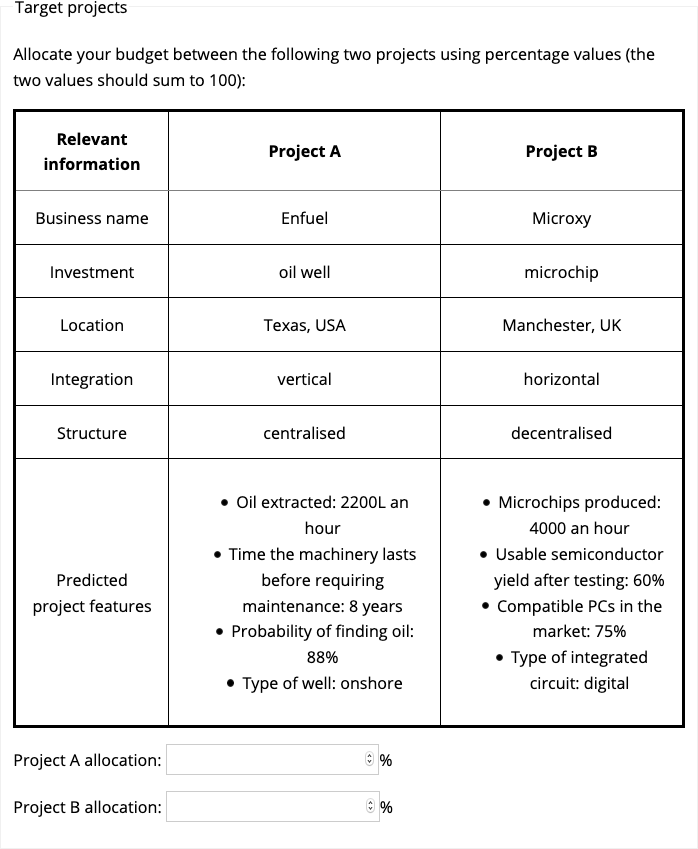
\includegraphics[width=1\linewidth]{thesis_files/figure-latex/project-allocation-anecdote-only-materials-anecdotes-1-1} \caption{Focal project display for the anecdote only condition in Experiment~1.}\label{fig:project-allocation-anecdote-only-materials-anecdotes-1}
\end{figure}



\begin{figure}
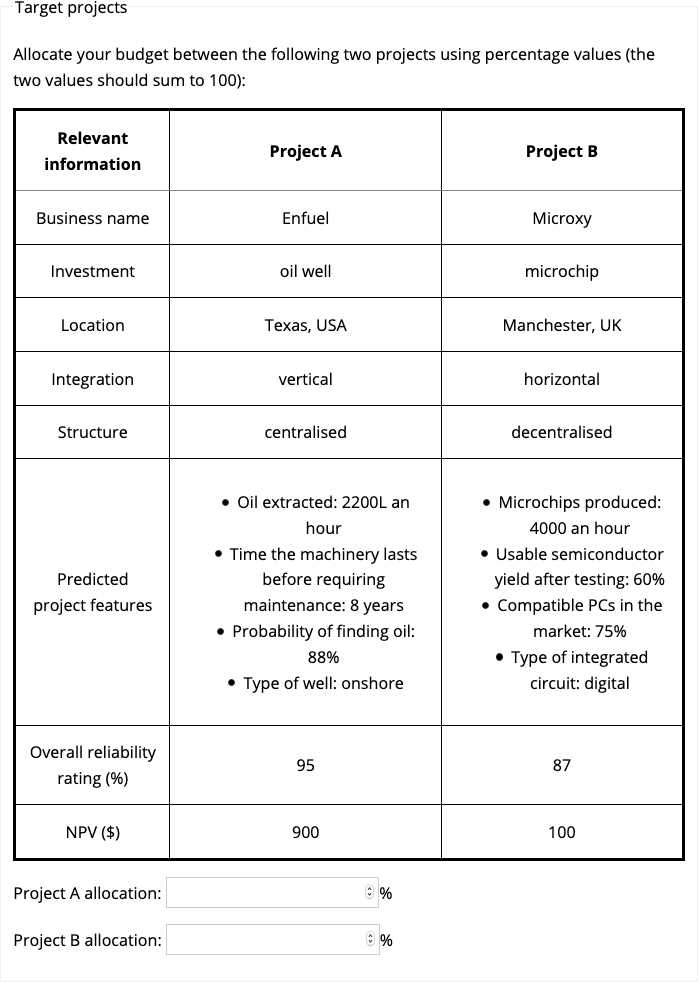
\includegraphics[width=1\linewidth]{thesis_files/figure-latex/project-allocation-statistics-materials-anecdotes-1-1} \caption{Focal project display for the statistics only, anecdote \& statistics, and anecdote \& enhanced statistics conditions in Experiment~1.}\label{fig:project-allocation-statistics-materials-anecdotes-1}
\end{figure}

\paragraph{Anecdote}

Participants that were presented with an anecdote (those in either the anecdote
only, anecdote \& statistics, or anecdote \& enhanced statistics conditions) saw a
description of a business project and an accompanying ``analysis.''
Figures~\ref{fig:anecdote-similarity-high-materials-anecdotes-1}
and~\ref{fig:anecdote-similarity-low-materials-anecdotes-1} show the anecdote
display for those in the high and low similarity conditions, respectively. The
project description had a similar layout to that of the focal projects. That is,
it contained information about the business name, location, integration, and
organisational structure of the business. It also detailed several predicted
features of the project. Underneath this description was a paragraph of text
that participants were told was an analysis of why the project failed. This text
referenced each of the features in the description in order to justify the
project failing.

Those in the high similarity condition saw a description of a project from a
business with the same type of investment as the target project (labelled
Project A). All categorical attributes were identical to those in this target
project, and the numerical attributes were all made to be lower. In the
analysis, the numerical attributes were explained to have failed because they
were not as high as certain cut-offs. Critically, these cut-offs were made to
all be higher than the relevant values in Project A. This was done to make sure
that the numerical attributes in the anecdote seem more relevant to those in
Project A. For instance, for Project A, oil extraction was 2200L an hour, for
the anecdote it was 2000L an hour, and the cutoff was 3000L an hour. As such, a
failure of the anecdote because of an insufficient oil extraction rated will
seem more relevant since they both share the state of being lower than the
cut-off in the analysis. Note, however, that there was uncertainty about the
generalisability of these cut-off values because the participants did not
receive a explicit indication of whether these values were meant to generalise
to other cases.



\begin{figure}
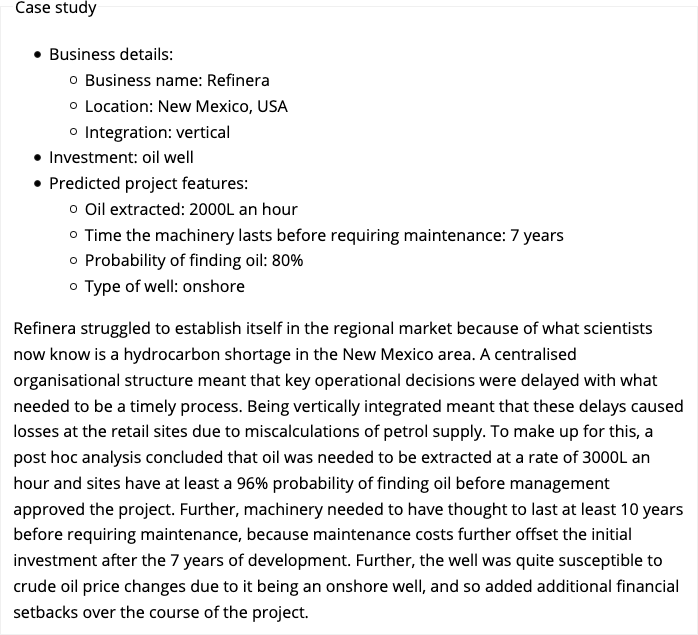
\includegraphics[width=1\linewidth]{thesis_files/figure-latex/anecdote-similarity-high-materials-anecdotes-1-1} \caption{Anecdote display for those in the high alignment condition in Experiment~1.}\label{fig:anecdote-similarity-high-materials-anecdotes-1}
\end{figure}



\begin{figure}
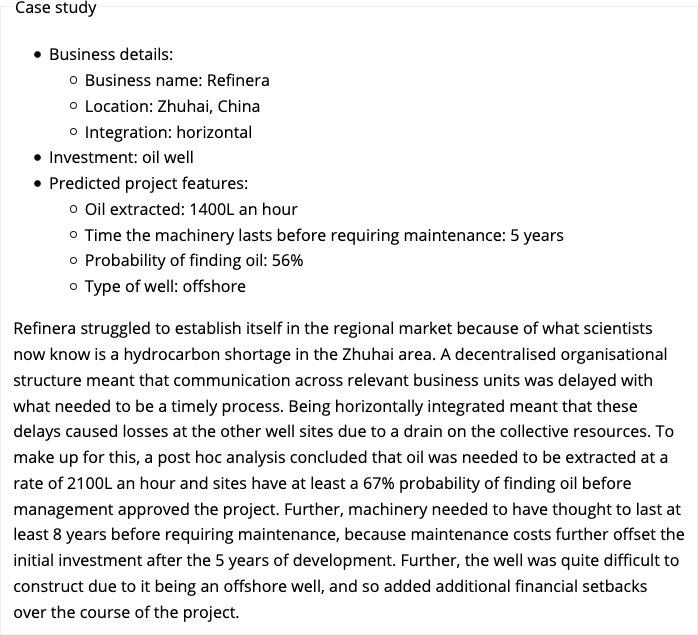
\includegraphics[width=1\linewidth]{thesis_files/figure-latex/anecdote-similarity-low-materials-anecdotes-1-1} \caption{Anecdote display for those in the low alignment condition in Experiment~1.}\label{fig:anecdote-similarity-low-materials-anecdotes-1}
\end{figure}

\paragraph{Follow-up questions}

Participants that saw the anecdote were subsequently presented with follow-up
questions. They were asked how similar they believe the anecdote was to the
target project, how relevant it was for their allocations, and how relevant it
would be for judgements about other projects of that type.
Figure~\ref{fig:follow-up-materials-anecdotes-1} in the appendix shows these
questions.

\subsubsection{Procedure}

Participants were introduced to the study through the general instructions and
the specific instructions relevant to their condition. They were then presented
with the allocation task, which included the anecdote analysis and description
(for those not in the statistics condition) and the focal projects description.
Those that saw an anecdote were subsequently shown the follow-up questions.

\hypertarget{results-anecdotes-1}{%
\subsection{Results}\label{results-anecdotes-1}}

\subsubsection{The effect of similarity on anecdotal bias}

Anecdotal bias was tested by comparing the statistics only condition with both
the high and the low similarity anecdote \& (not enhanced) statistics conditions.
Figure~\ref{fig:plot-anecdotes-1-allocation-combined} shows these data. The
omnibus one-way ANOVA test of these three conditions was significant,
\(F(2, 118) = 4.19\), \(p = .018\), \(\hat{\eta}^2_p = .066\). Planned comparisons revealed that
participants allocated more to the target project when seeing only statistics
than when seeing the high similarity anecdote with statistics,
\(\Delta M = -12.31\), 95\% CI \([-21.53,~-3.09]\), \(t(118) = -2.64\), \(p = .009\); but not compared
to seeing the low similarity anecdote with statistics,
\(\Delta M = -1.48\), 95\% CI \([-10.75,~7.80]\), \(t(118) = -0.31\), \(p = .753\). These findings
provide evidence of anecdotal bias only in the high similarity condition.



\begin{figure}
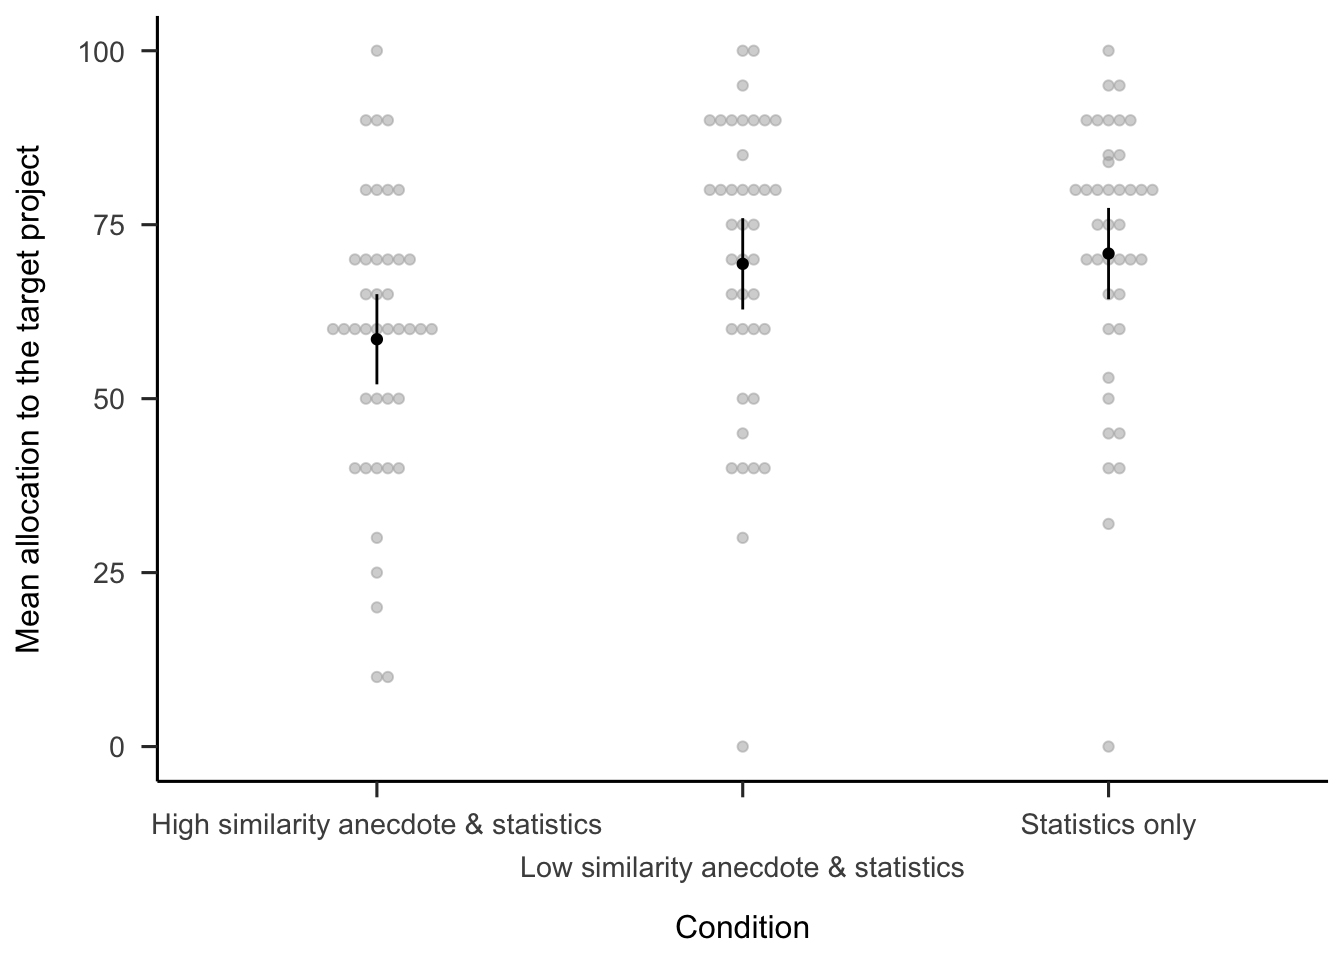
\includegraphics[width=1\linewidth]{thesis_files/figure-latex/plot-anecdotes-1-allocation-combined-1} \caption{Mean allocation to the target project. Error bars represent 95\% confidence intervals.}\label{fig:plot-anecdotes-1-allocation-combined}
\end{figure}

\subsubsection{The effect of enhanced statistics}

The effect of enhanced statistics was investigated by comparing the conditions
in which participants saw an anecdote with statistics to the conditions in which
they saw the same, but with enhanced statistics.
Figure~\ref{fig:plot-anecdotes-1-allocation} shows these data. The two-way
interaction between similarity and the two types of the anecdote \& statistics
condition was not significant,
\(M = 3.89\), 95\% CI \([-8.86,~16.65]\), \(t(238) = 0.60\), \(p = .548\). Further, the main
effect of anecdote \& statistics condition (averaging over similarity) was also
not significant, \(\Delta M = -0.12\), 95\% CI \([-6.50,~6.26]\), \(t(238) = -0.04\), \(p = .971\). This
suggests that providing participants with instructions on how to think
statistically is not sufficient to facilitate a focus on statistics.



\begin{figure}
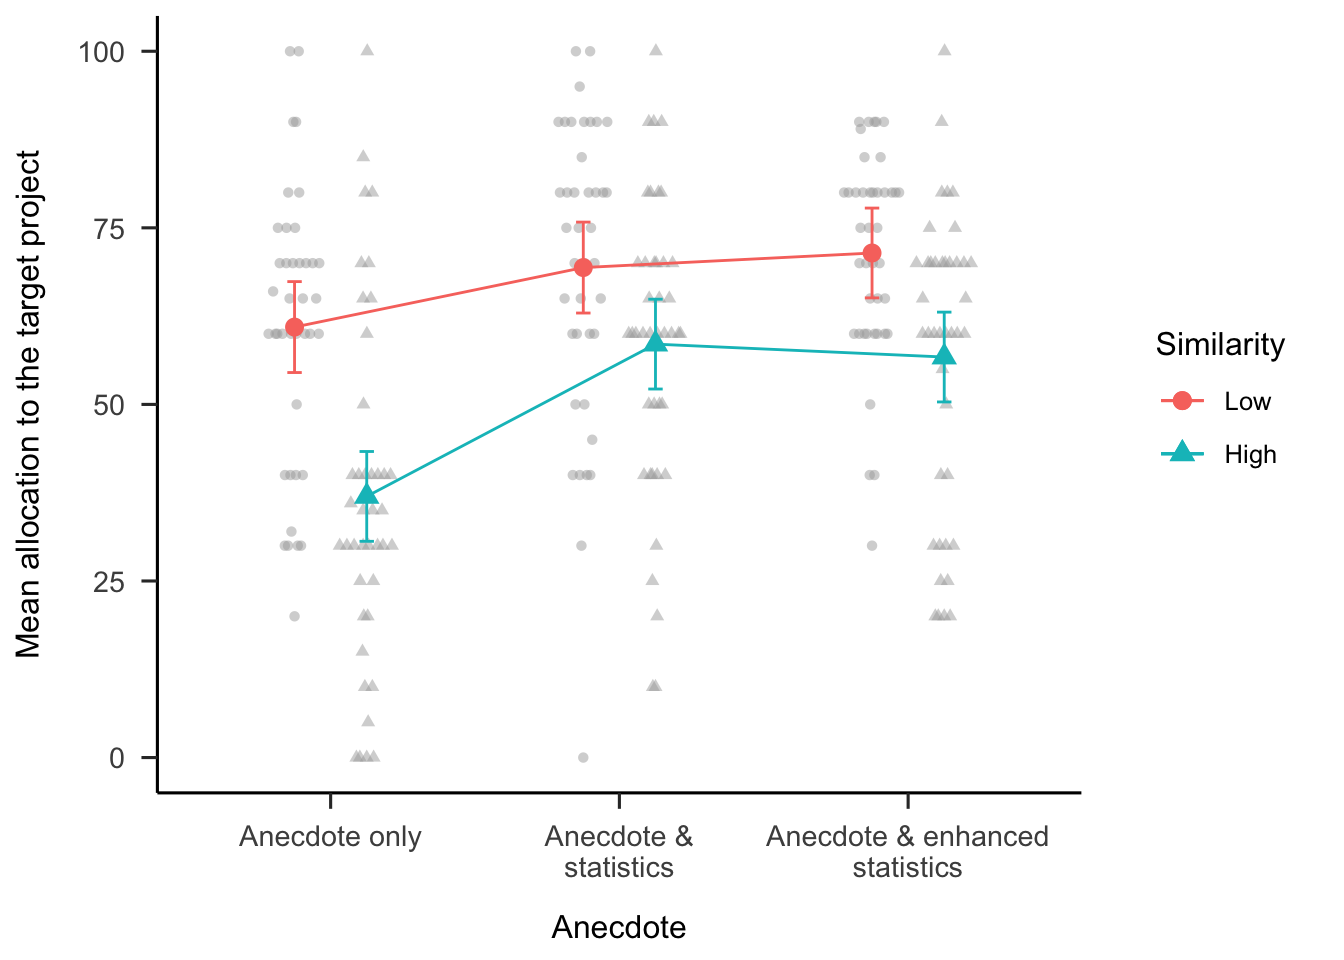
\includegraphics[width=1\linewidth]{thesis_files/figure-latex/plot-anecdotes-1-allocation-1} \caption{Mean allocation to the target project. Error bars represent 95\% confidence intervals.}\label{fig:plot-anecdotes-1-allocation}
\end{figure}

\subsubsection{The effect of statistics}

A two-way ANOVA was conducted to investigate the interaction of similarity (low
and high) and anecdote condition (anecdote only and statistics \& anecdote,
excluding the anecdote \& enhanced statistics condition).
Figure~\ref{fig:plot-anecdotes-1-allocation} shows these data. This identified
the role of statistics in people's allocations. The interaction between anecdote
condition and similarity (excluding the enhanced statistics condition) was
significant, \(M = -13.14\), 95\% CI \([-25.93,~-0.34]\), \(t(238) = -2.02\), \(p = .044\).
Specifically, the difference between allocations when only seeing an anecdote
and seeing the anecdote with statistics was greater when the anecdote was
similar,
\(\Delta M = -21.56\), 95\% CI \([-32.33,~-10.80]\), \(t(238) = -4.72\), \(p < .001\); compared to when it
was dissimilar, \(\Delta M = -8.43\), 95\% CI \([-19.32,~2.47]\), \(t(238) = -1.82\), \(p = .164\). These
findings provide evidence of partial anecdotal bias in the high similarity
condition, since the anecdote \& statistics condition was lower than the
statistics only condition (shown above), but higher than the anecdote only
condition.

\subsubsection{Relevance ratings}

Regression analyses were conducted to determine the relationship between
allocations and the follow-up relevance ratings. As seen in
Figure~\ref{fig:plot-anecdotes-1-lm-allocation-relevance-specific-alignment}
the specific relevance ratings interacted with similarity condition,
\(b = -2.84\), 95\% CI \([-4.80, -0.87]\), \(t(240) = -2.85\), \(p = .005\). It appears
that specific relevance ratings were related to allocations, but only in the
high similarity condition. Further, there were no significant associations with
the general relevance ratings. This suggests that people were reasoning about
the connection between the anecdote and target, as opposed to simply reacting to
the failed project and associating that with that project's industry.



\begin{figure}
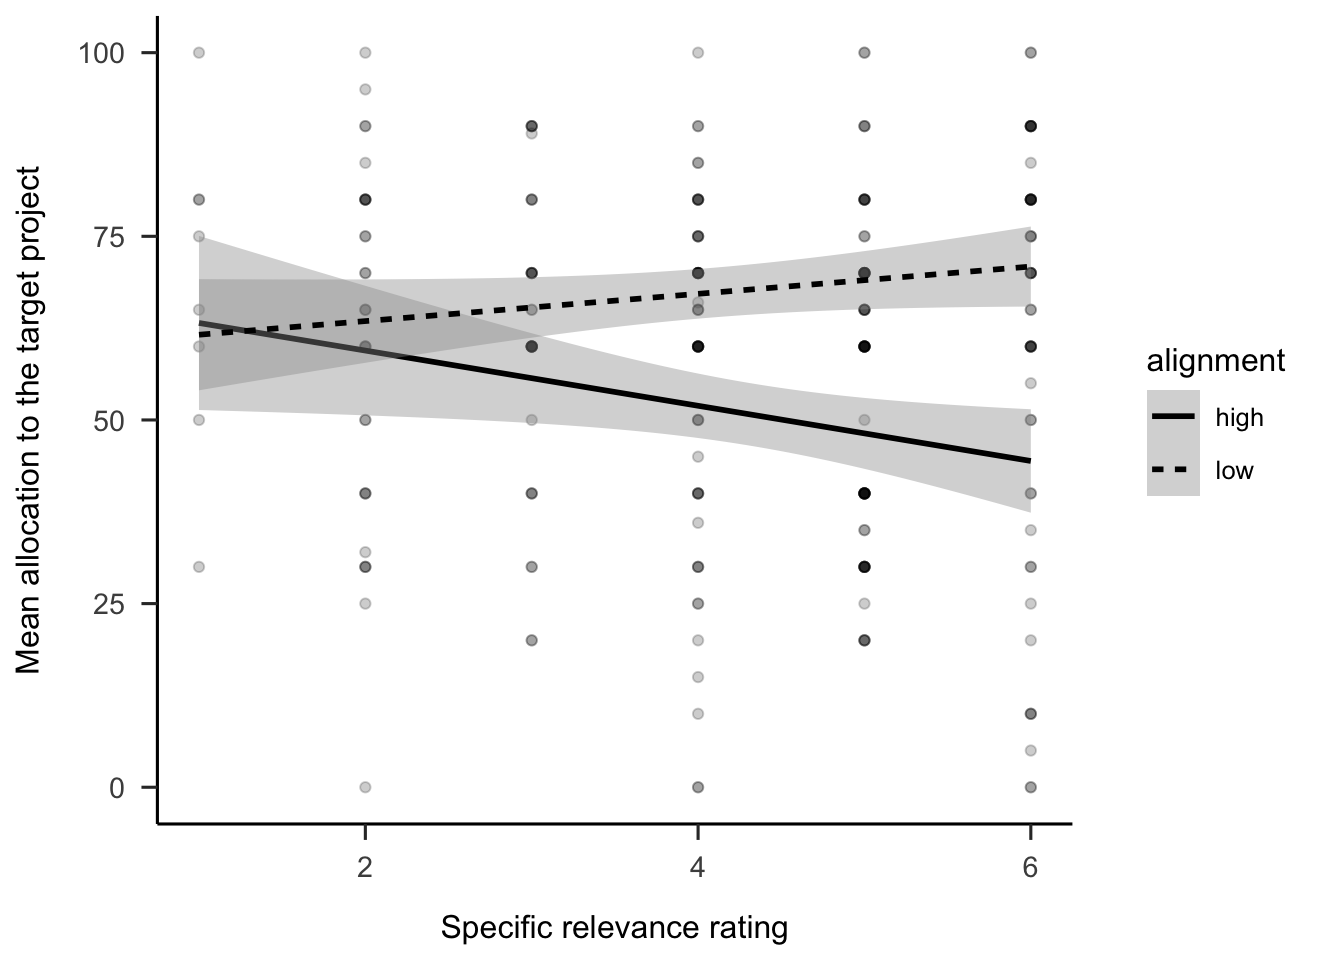
\includegraphics[width=1\linewidth]{thesis_files/figure-latex/plot-anecdotes-1-lm-allocation-relevance-specific-alignment-1} \caption{Mean allocations to the target project, by specific relevance rating and similarity condition.}\label{fig:plot-anecdotes-1-lm-allocation-relevance-specific-alignment}
\end{figure}

\subsection{Discussion}

Hypothesis~\ref{hyp:anecdote-similarity-anecdotes-1} was supported.
Participants allocated less capital when seeing the anecdote with statistics
than when seeing the statistics alone. This effect was moderated by similarity,
however, as it was seen in the high similarity condition, but not in the low
similarity condition. This shows that while anecdotal bias exists when the
anecdote is similar, participants are not influenced when the causal mechanisms
do not match. Contrary to Hypothesis~\ref{hyp:statistics-anecdotes-1}, despite
being influenced by the anecdote, participants still made some use of the
statistics. This is different from \textcite{wainberg2013}, who found no difference
between an anecdote only and an anecdote \& statistics condition, indicating a
complete effect of anecdotal bias.
Hypothesis~\ref{hyp:enhanced-statistics-anecdotes-1} was also not supported, as
the added enhanced statistical language used to encourage participants to use
the statistical information did not contribute to reducing participants'
reliance on anecdotes.

Experiment~1 was limited because it only considered an anecdote with a
\emph{negative} valence. That is, the case study was of a project that failed. In
real life, however, these case studies are often ones with \emph{positive} valence.
That is, a story of a successful company. In fact, in business, the anecdotes
that are used might be more likely to be positive, because of survivorship bias.
\textcite{jaramillo2019} found an anecdotal bias effect in negative anecdotes, but not in
positive anecdotes. This may be because the stimuli consisted of medical
decisions and in this domain a loss of health may be felt stronger than an
equivalent gain of health. Experiment~2 added a condition with a positive
anecdote, in order to investigate whether anecdote valence will impact the
anecdotal bias effect.

It was unclear if the effects found in Experiment~1 were related to
participants' perceptions of the type of sampling used in selecting the
anecdotes. The instructions in Experiment~1 did not explain how the anecdote
displayed to participants was chosen. Whether sampling is believed to be
intentional or random has been shown to affect people's decision-making \autocite[e.g.,][]{hayes2019}. In the case of the current experiments, the sampling assumption
changes the extent to which it is rational to use the anecdote or not. It may be
rational to choose the anecdote over the aggregated data if 1. the anecdote was
not sampled randomly from the pool of anecdotes, and 2. the anecdote is more
similar to the target project than any of the other anecdotes in the pool in
relevant ways. That is, if the anecdote was chosen because of its high relevance
to the target project, it would be irrational to ignore it. In Experiment~1 it
was unclear whether participants might have held these beliefs. In order to
control for these assumptions, in Experiment~2, text was added to the
instructions that clarified that the anecdote 1. was sampled randomly from the
pool of anecdotes, and 2. is not significantly more similar to the target
project than any of the other anecdotes in the pool.

\hypertarget{anecdotes-2}{%
\section{Experiment~2}\label{anecdotes-2}}

Experiment~1 replicated the anecdotal bias effect found in the literature. That
is, people used an anecdote more when presented with conflicting statistics than
with anecdote alone and less than with statistics alone. However, anecdote
similarity moderated this effect, such that anecdotal bias was stronger when the
anecdote was similar to the current task, than when it was dissimilar.
Experiment~1 only used a negative anecdote because previous research found
anecdotal bias for negative, but not for positive anecdotes \autocite{jaramillo2019}.
However, \textcite{jaramillo2019} considered medical decision-making, so this effect of
anecdote valence may be different in a business context. In the study, the
positive anecdote involved a treatment that led to a reduction in symptoms and
the negative anecdote involved symptoms persisting. This framing might mean
participants represented the positive anecdote as a return to a reference point
and the negative anecdote as a continuation of a reduction in well-being,
relative to the reference point. In business, however, both successful and
failed business projects represents a deviation from a reference point. To test
this difference further, Experiment~2 added an anecdote valence manipulation

In order to increase the experiment's power, anecdote valence and anecdote
similarity were manipulated within-subjects. Further, Experiment~2 did not
include the anecdote \& enhanced statistics manipulation, because Experiment~1
did not find evidence for its effect. All participants saw the statistics only
condition, as it did not contain an anecdote, and therefore did not need to be
manipulated between-subjects. Each participant therefore saw five displays: one
display for the statistics only condition; and four displays for either the
anecdote only condition, or the anecdote \& statistics condition. These four
anecdote displays consisted of the similarity (low and high) \(\times\) valence
(negative and positive) conditions.

Experiment~1 did not clarify certain assumptions about the distribution from
which the anecdote was sampled. In Experiment~2, participants were told that the
anecdote was sampled randomly and that it was not uniquely similar to the target
project. This should lead to a reliance on the statistical evidence, regardless
of the anecdote's similarity. However, people often struggle to use statistical
concepts presented descriptively, as seen in the enhanced statistics condition
in Experiment~1, the variance neglect in Chapter~\ref{alignment}, and the lack
of risk aggregation in descriptive risky choice as in
Chapter~\ref{aggregation}. Therefore, it was expected that the effects of
Experiment~1 will replicate in the negative valence condition. Further it was
expected that there will be a reverse effect in the positive valence condition.
The appendix shows a simulation of the hypothesised effects (see
Figures~\ref{fig:plot-simulation-anecdotes-2-negative}
and~\ref{fig:plot-simulation-anecdotes-2-positive}). Therefore, Experiment~2
tested the following:

\begin{hypothesis}[Overall effect]
\protect\hypertarget{hyp:three-way-anecdotes-2}{}{\label{hyp:three-way-anecdotes-2} \iffalse (Overall effect) \fi{} }Three-way interaction of similarity \(\times\) valence \(\times\) anecdote,
excluding statistics only
\end{hypothesis}

The main effect of interest was the moderation of anecdotal bias by similarity.
Therefore, as well as again testing
Hypothesis~\ref{hyp:anecdote-similarity-anecdotes-1} for negative anecdotes,
Experiment~2 tested the following:

\begin{hypothesis}[Anecdotal bias moderated by similarity for positive anecdotes]
\protect\hypertarget{hyp:anecdote-similarity-anecdotes-2}{}{\label{hyp:anecdote-similarity-anecdotes-2} \iffalse (Anecdotal bias moderated by similarity for positive anecdotes) \fi{} }For positive anecdotes, allocations will be higher in the statistics only
condition than in both the anecdote \& statistics conditions (high and low
similarity). Within these two anecdote \& statistics conditions, allocations will
be higher when the anecdote is similar than when it is dissimilar.
\end{hypothesis}

Contrary to both \textcite{wainberg2013} and Hypothesis~\ref{hyp:statistics-anecdotes-1},
Experiment~1 found that participants do somewhat integrate statistics in their
decisions. This effect was expected to replicate in Experiment~2. Therefore,
Experiment~2 tested the following:

\begin{hypothesis}[Effect of statistics for negative anecdotes]
\protect\hypertarget{hyp:statistics-negative-anecdotes-2}{}{\label{hyp:statistics-negative-anecdotes-2} \iffalse (Effect of statistics for negative anecdotes) \fi{} }For negative anecdotes, allocations will be higher for the high similarity
anecdote \& statistics condition than for the high similarity anecdote only
condition.
\end{hypothesis}

\begin{hypothesis}[Effect of statistics for positive anecdotes]
\protect\hypertarget{hyp:statistics-positive-anecdotes-2}{}{\label{hyp:statistics-positive-anecdotes-2} \iffalse (Effect of statistics for positive anecdotes) \fi{} }For positive anecdotes, allocations will be higher for the high similarity
anecdote only condition than for the high similarity statistics \& anecdote
condition.
\end{hypothesis}

\subsection{Method}

\subsubsection{Participants}

Ninety-six people (50 female) were recruited from the online recruitment platform Prolific. Participants were compensated at a rate of £5 an hour. The average age was 41.69 (\emph{SD} = 11.29, \emph{min} = 27, \emph{max} = 74). Participants reported an average of 7.19 (\emph{SD} = 8.34, \emph{min} = 0, \emph{max} = 43) years of work in a business setting, and an average of 3.91 (\emph{SD} = 7.67, \emph{min} = 0, \emph{max} = 50) years of business education. The mean completion time was 14.98 (\emph{SD} = 8.84, \emph{min} = 2.57, \emph{max} = 58.71) minutes.~Table~\ref{tab:condition-allocation-anecdotes-2}
shows the between-subjects condition allocation. Similarity and valence were
manipulated within-subjects. Therefore, each participant was in one of two
between-subjects anecdote conditions, and saw five displays (statistics only,
and one for each of the four similarity and valence conditions).
Appendix~\ref{power-analysis-anecdotes-2} describes the power analysis
conducted to arrive at this sample size.

\begin{table}[tbp]

\begin{center}
\begin{threeparttable}

\caption{\label{tab:condition-allocation-anecdotes-2}Experiment 2 group allocation.}

\begin{tabular}{ll}
\toprule
Anecdote between & \multicolumn{1}{c}{N}\\
\midrule
Anecdote \& statistics & 48\\
Anecdote only & 48\\
Total & 96\\
\bottomrule
\end{tabular}

\end{threeparttable}
\end{center}

\end{table}

\subsubsection{Materials}

\paragraph{Instructions}

Participants were shown similar instructions to Experiment~1 (see
Section~\ref{instructions-materials-anecdotes-1}). The general instructions
page included a test of the basic information expressed in the instructions.
This test also functioned as an attention check. As in Experiment~1,
participants also saw instructions that were specific to their condition. These
were shown on the same page as the rest of the project display, above the case
study and focal projects. The instructions clarified both that the anecdote was
sampled randomly and that the anecdotes in the pool were all equally similar to
the target project. Appendix~\ref{instructions-materials-anecdotes-2-appendix}
shows the instructions used in Experiment~2.

\hypertarget{allocation-anecdotes-2}{%
\paragraph{Allocation task}\label{allocation-anecdotes-2}}

As in Experiment~1, the allocation task included a description and analysis of
an anecdote (except for those in the anecdote only condition) and a project
display with a table describing the two focal projects.
Figures~\ref{fig:project-allocation-anecdote-valence-negative-similarity-low-materials-anecdotes-2}
and~\ref{fig:project-allocation-target-valence-negative-similarity-low-materials-anecdotes-2}
show the anecdote and focal projects, respectively, for the negative valence
low similarity condition.
Figures~\ref{fig:project-allocation-anecdote-valence-positive-similarity-high-materials-anecdotes-2}
and~\ref{fig:project-allocation-target-valence-positive-similarity-high-materials-anecdotes-2}
show the anecdote and focal projects, respectively, for the positive valence
high similarity conditions. In the statistics only condition, participants only
saw the focal projects display. Appendix~\ref{allocation-anecdotes-2-appendix}
details the counterbalancing and randomisation used in the experiment.



\begin{figure}

\includegraphics[width=1\linewidth]{thesis_files/figure-latex/project-allocation-anecdote-valence-negative-similarity-low-materials-anecdotes-2-1} \caption{An example of the anecdote display in the negative valence, low similarity condition of Experiment~2.}\label{fig:project-allocation-anecdote-valence-negative-similarity-low-materials-anecdotes-2}
\end{figure}



\begin{figure}
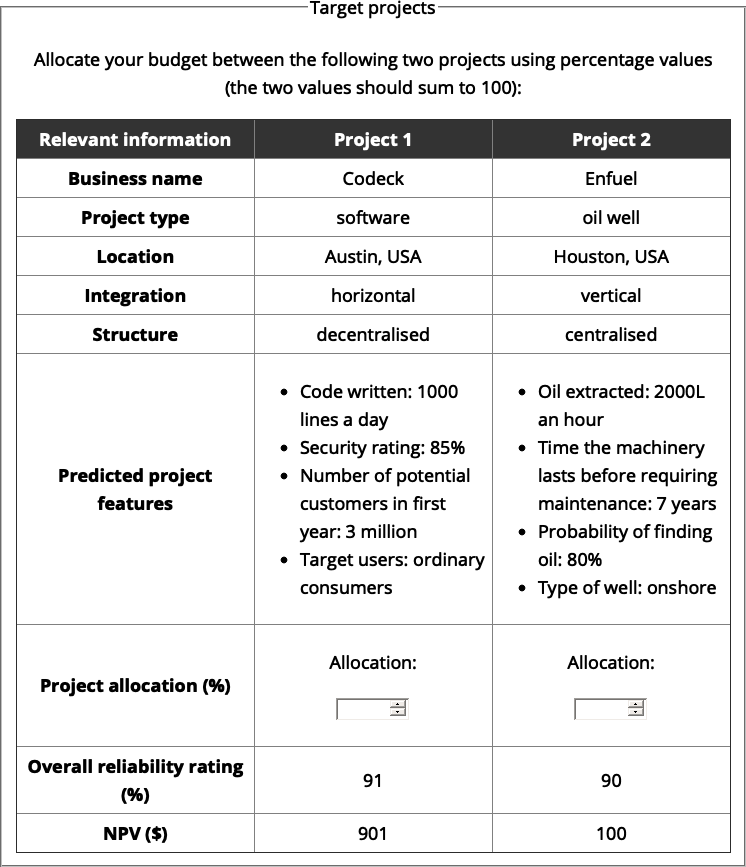
\includegraphics[width=1\linewidth]{thesis_files/figure-latex/project-allocation-target-valence-negative-similarity-low-materials-anecdotes-2-1} \caption{An example of the focal projects in the negative valence, low similarity condition of Experiment~2.}\label{fig:project-allocation-target-valence-negative-similarity-low-materials-anecdotes-2}
\end{figure}



\begin{figure}

\includegraphics[width=1\linewidth]{thesis_files/figure-latex/project-allocation-anecdote-valence-positive-similarity-high-materials-anecdotes-2-1} \caption{An example of an anecdote display in the positive valence, high similarity condition of Experiment~2.}\label{fig:project-allocation-anecdote-valence-positive-similarity-high-materials-anecdotes-2}
\end{figure}



\begin{figure}
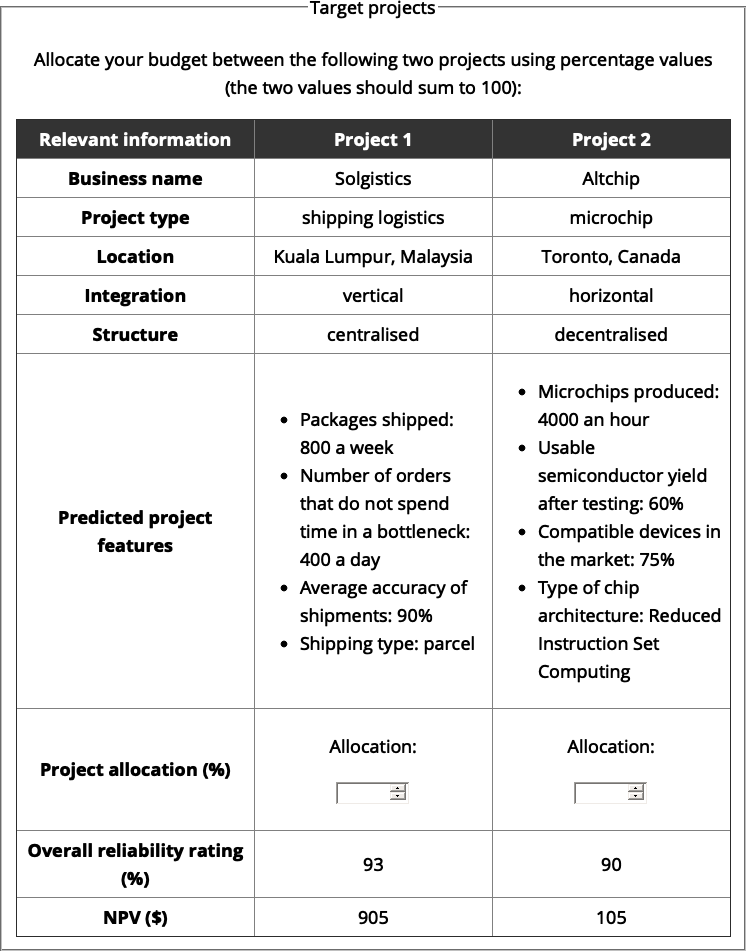
\includegraphics[width=1\linewidth]{thesis_files/figure-latex/project-allocation-target-valence-positive-similarity-high-materials-anecdotes-2-1} \caption{An example of the focal projects in the positive valence, high similarity condition of Experiment~2.}\label{fig:project-allocation-target-valence-positive-similarity-high-materials-anecdotes-2}
\end{figure}

\paragraph{Interstitial}

Before each display, participants saw an ``interstitial'' page, whose role was 1.
to introduce the next display, and 2. to provide an attention check (not
required to answer, so can be skipped if the interstitial text isn't read). See
Figure~\ref{fig:interstitial-materials-anecdotes-2} in the appendix for an
example.

\paragraph{Follow-up questions}

Participants were shown similar follow-up questions as in Experiment~1, except
that here the rating scales were 1-7, instead of 1-6. See
Figure~\ref{fig:follow-up-materials-anecdotes-2} in the appendix for an example
of the follow-up questions display.

\subsubsection{Procedure}

Participants were introduced to the study through the general instructions page.
They then saw five sets of two pages (in randomised order). Each set contained
two pages: the allocation task and a follow-up questions page (except for the
anecdotes only condition, in which participants did not see the follow-up
questions page). Each allocation task page contained specific instructions
relevant to the condition, followed by the anecdote analysis and description,
and the description for the two focal projects. The only exception was the
statistics only display, for which there was no anecdote description or
analysis.

\subsection{Results}

Only the data that were relevant to the Experiment~2 hypotheses are reported
here. See Appendix~\ref{results-anecdotes-2-appendix} for manipulation check
analyses, and analyses of the follow-up rating data.

\subsubsection{Overall effect of manipulations}

As seen in Figure~\ref{fig:plot-anecdotes-2-allocation}, the similarity
\(\times\) valence \(\times\) anecdote interaction (excluding the statistics only
condition) was not significant,
\(F(1, 94) = 3.42\), \(p = .067\), \(\hat{\eta}^2_p = .035\). However,
the similarity \(\times\) valence interaction was significant,
\(F(1, 94) = 76.41\), \(p < .001\), \(\hat{\eta}^2_p = .448\), as was the anecdote
\(\times\) valence interaction,
\(F(1, 94) = 10.11\), \(p = .002\), \(\hat{\eta}^2_p = .097\). The analyses below investigated the specific hypothesised effects.



\begin{figure}
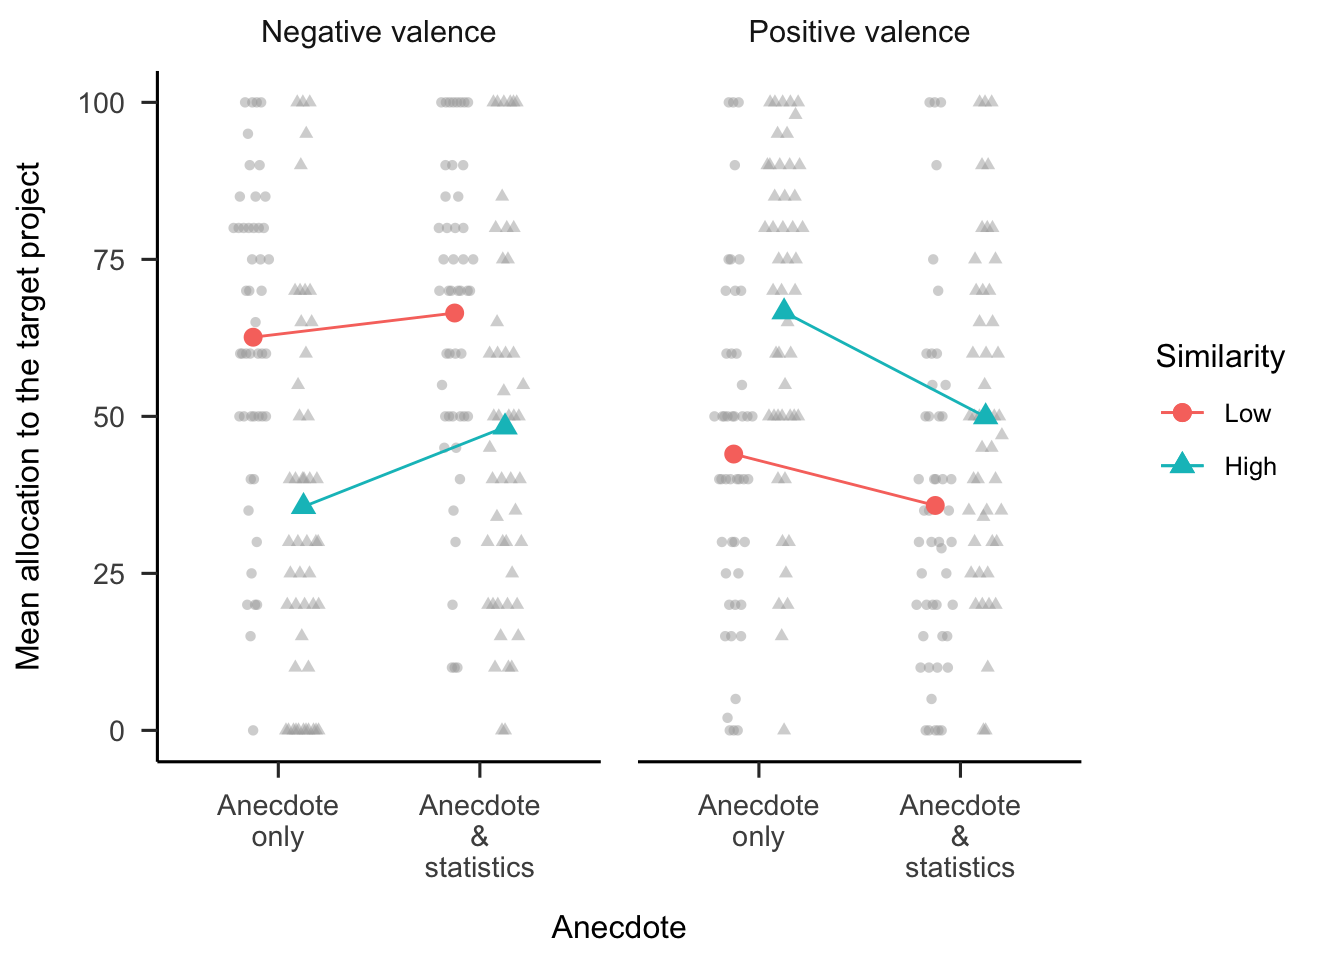
\includegraphics[width=1\linewidth]{thesis_files/figure-latex/plot-anecdotes-2-allocation-1} \caption{Mean allocation to the target project in Experiment~2. Error bars represent 95\% confidence intervals, calculated from the model-based standard error. Note that due to the mixed within-between design, these error bars do not permit inferences ``by eye'' across repeated-measures factors.}\label{fig:plot-anecdotes-2-allocation}
\end{figure}

\subsubsection{Anecdotal bias moderated by similarity}

To investigate whether anecdotal bias was moderated by similarity, a difference
measure was calculated between each participant's allocation to the statistics
only condition and their allocation to each of the two anecdote \& statistics
conditions conditions (high and low similarity). The statistics only comparison
value was different for each valence condition to create equivalent comparisons.
For negative valence, the allocation to the high NPV project was used; while for
positive valence, the allocation to the low NPV project was used.
Figure~\ref{fig:plot-anecdotes-2-allocation-difference} shows these data. The
similarity \(\times\) valence interaction was significant,
\(F(1, 47) = 30.66\), \(p < .001\), \(\hat{\eta}^2_p = .395\), as was the
main effect of valence,
\(F(1, 47) = 9.85\), \(p = .003\), \(\hat{\eta}^2_p = .173\). The main effect of
similarity was not significant,
\(F(1, 47) = 0.53\), \(p = .469\), \(\hat{\eta}^2_p = .011\).

The interaction was analysed further by comparing the two similarity conditions
for each valence condition. For negative anecdotes, the allocation difference
was greater when the anecdote was similar to the target than when it was
dissimilar, \(\Delta M = -18.17\), 95\% CI \([-26.17,~-10.17]\), \(t(93.80) = -4.51\), \(p < .001\). For
positive anecdotes, the allocation difference was greater when the anecdote was
dissimilar to the target than when it was similar,
\(\Delta M = 14.10\), 95\% CI \([6.10,~22.11]\), \(t(93.80) = 3.50\), \(p = .001\). This provides
evidence for the moderation of anecdotal bias by similarity for both negative
and positive anecdotes. People seem to be sensitive to the relevance of the
anecdote to the target problem.



\begin{figure}
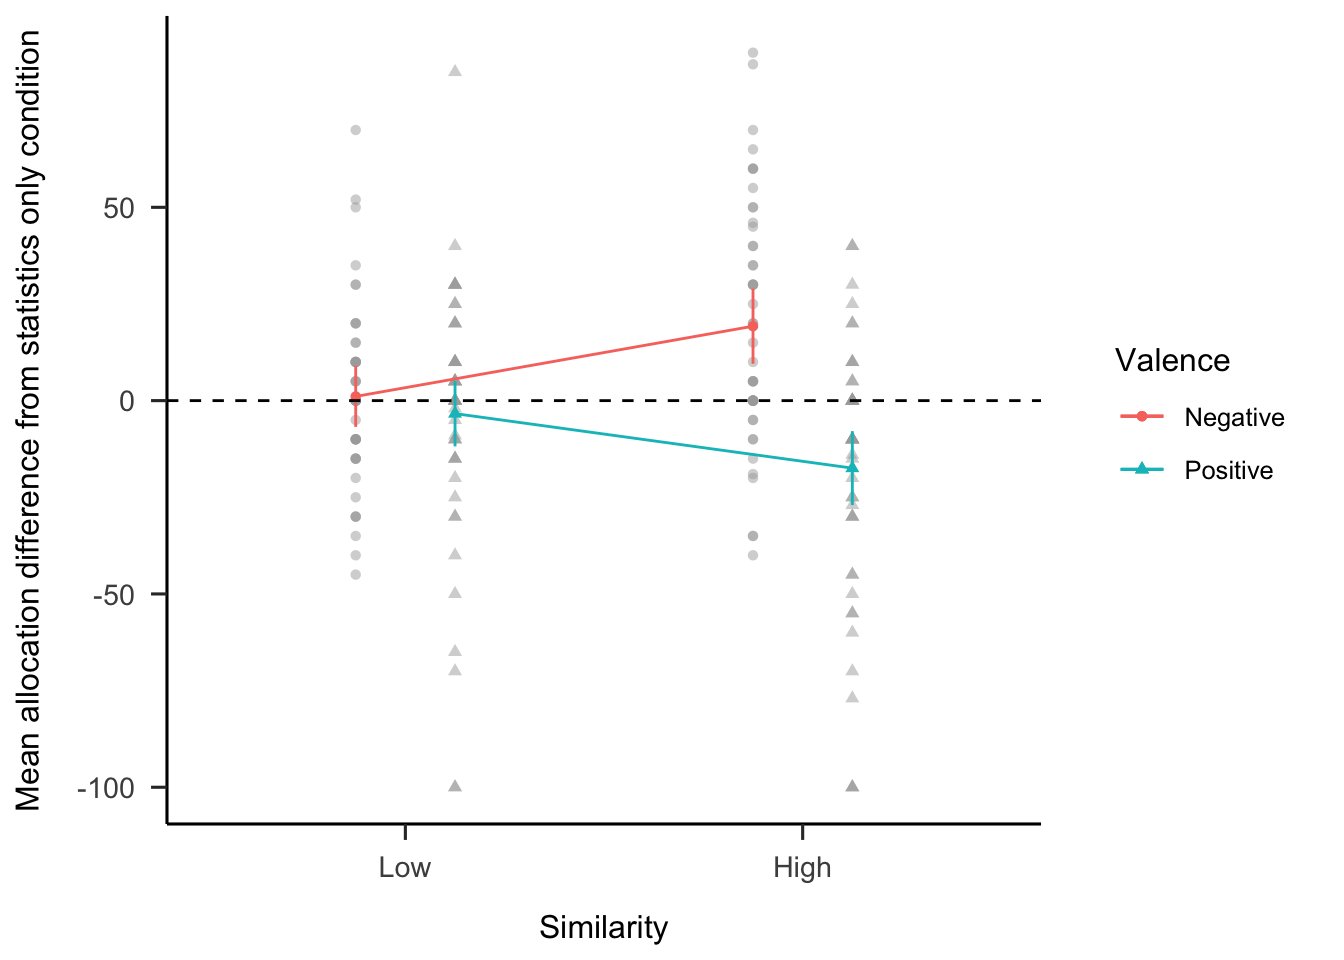
\includegraphics[width=1\linewidth]{thesis_files/figure-latex/plot-anecdotes-2-allocation-difference-1} \caption{Mean allocation difference in Experiment~2 between the statistics only condition and the anecdote \& statistics condition. The horizontal dashed line shows the point in which the two allocations were equivalent. Values that are higher than this line represent participants that allocated more when seeing only the statistics than when seeing the statistics with an anecdote. Error bars represent 95\% confidence intervals, calculated from the within-subjects SEs using the method from \textcite{cousineau2014}.}\label{fig:plot-anecdotes-2-allocation-difference}
\end{figure}

\subsubsection{Effect of statistics}

As in Experiment~1, Experiment~2 investigated the extent to which the
statistical information influenced participants' allocations. As seen in
Figure~\ref{fig:plot-anecdotes-2-allocation}, for negative anecdotes,
participants allocated more to the high similarity anecdote \& statistics project
than those in the high similarity anecdote only condition,
\(\Delta M = -12.67\), 95\% CI \([-23.53,~-1.81]\), \(t(336.36) = -2.29\), \(p = .022\).
When in the positive valence condition, they allocated more to the high
similarity anecdote only condition than those in the high similarity anecdote \&
statistics condition,
\(\Delta M = 16.71\), 95\% CI \([5.85,~27.57]\), \(t(336.36) = 3.03\), \(p = .003\).
This provides evidence for the influence of statistics on participants'
allocations for both negative and positive anecdotes.

\subsection{Discussion}

Hypotheses~\ref{hyp:anecdote-similarity-anecdotes-1}
and~\ref{hyp:anecdote-similarity-anecdotes-2} were supported, as participants
showed a stronger anecdotal bias effect when the anecdote was more similar to
the target project, for both positive and negative anecdotes. Further, as per
Hypotheses~\ref{hyp:statistics-negative-anecdotes-2}
and~\ref{hyp:statistics-positive-anecdotes-2}, participants incorporated the
statistical information into their judgements, for both negative and positive
anecdotes.

Experiment~2 therefore found that, unlike in the medical domain, the effect of
anecdotes in financial decision-making does not depend on anecdote valence.
Further, as in Experiment~1, and unlike in \textcite{wainberg2013}, the anecdotal bias
effect does not seem to be complete, with statistics still playing some role in
participants' decisions despite the effect of the anecdote.

\section{General discussion}

Most of the hypotheses were supported. This chapter found that, in a capital
allocation context, people's decisions are influenced by anecdotes even when
aggregated data are available. There were three novel findings: 1. the anecdotal
bias effect was only seen when participants considered the anecdote as
sufficiently relevant to the target project, 2. participants integrated
statistics in their decisions, and 3. these effects were found in both negative
and positive anecdotes.

The first novel finding from these experiments was that participants moderated
their use of anecdotal evidence. Specifically, when the anecdote appeared to be
causally relevant, participants used it in their decisions. However, when it
appeared irrelevant, participants relied on statistics almost entirely. The
findings in the high similarity condition are largely congruent with findings
from other work investigating anecdotal bias in business decision-making. As in
\textcite{wainberg2013} and \textcite{wainberg2018}, this chapter found that people allocated less
capital to a project that is successful according to statistical evidence
co-presented with contradictory similar anecdote, than to a project with the
statistics alone.

It seems that participants made the distinction between the low and high
similarity conditions based on the underlying structure of the anecdote. The low
similarity condition always consisted of the same project type, for each domain,
as in the high similarity condition. For instance, in one variation, both the
high and low similarity anecdotes involved oil well projects. However, the high
similarity anecdotes also matched with the target project on a number of
specific features. This means that participants were sensitive to the specific
information presented to them in the anecdote description and analysis, and did
not simply use the project type for their inferences. Further, participants'
answers to the follow up questions indicated that they did not consider the
anecdote to be necessarily relevant to other projects from the same industry. In
other words, participants did not appear to carelessly use anecdotal evidence in
their decisions, but instead appeared to carefully consider the anecdote based
on its particular causal structure.

The second novel finding from these experiments was that participants that saw
the statistics with anecdotal evidence did not completely disregard the
statistical measures. \textcite{wainberg2013} found a complete effect of anecdotal bias,
because in their study the anecdote only and anecdote \& statistics conditions
were equivalent. This meant that the statistics they provided had a negligible
effect on participants' decisions. The experiments in this chapter, on the other
hand, showed a partial anecdotal bias effect, seen as a difference in
allocations between the anecdote only and anecdote \& statistics conditions. It
seems as if participants integrated the anecdotal information with the
statistical information. This suggests that people's evaluation of evidence
might be more sensitive than previously thought.

The discrepancy between these results and those in \textcite{wainberg2013} might be a
result of the sampled population. Since \textcite{freling2020} found a stronger effect of
anecdote when decisions were more personally relevant, the manager sample in
\textcite{wainberg2013} may have simply been more personally invested in the task than the
laypeople in the experiments in this chapter. Similarly, \textcite{yang2015} found that
anxiety increases anecdotal bias in risky choice. The discrepancy might also,
however, be due to the anecdote \& statistics condition not being equivalent
between \textcite{wainberg2013} and the present work. Specifically, the statistics shown
in the anecdote \& statistics condition in \textcite{wainberg2013} were not the same ones
that were shown in the same study's statistics only condition, unlike in both
the present experiments and \textcite{wainberg2018}. Instead, it was the anecdote \&
enhanced statistics condition that contained the same statistics as in the
statistics only condition. This suggests that people only integrate statistics
when they are sufficiently clear and no further interpretation is required.

The third novel finding from these experiments was that anecdotal bias was found
in both negative and positive anecdotes. Most studies in the literature
considered anecdotes that involve an example with negative consequences (a
\emph{negative} anecdote). For instance, a medication that does not treat the
symptoms of an illness. However, there is not much work in the literature that
involves an anecdote with positive consequences (a \emph{positive} anecdote).
\textcite{jaramillo2019} found an asymmetry in the effect of the anecdote, such that the
effect was stronger when a person in a description did not get better after a
medication (negative), compared to when they did get better (positive). The
present experiments found a more symmetrical effect, such that both the effects
of the moderated anecdotal bias and the influence of statistics were found in
both valence conditions.

The difference between the findings from this chapter and those from
\textcite{jaramillo2019} might be due to the negative anecdote in their experiment
representing a persistence in a negative shift from the status quo (of not being
sick). In the business domain, both the positive and negative anecdotes
represent shifts from the status quo (of the company's financial position).
Regardless, it is still surprising not to find an asymmetry because of the
predictions of prospect theory. Loss aversion suggests that participants would
have avoided the projects associated with the negative anecdotes more than they
would have chosen those associated with the positive anecdotes. On the other
hand, each choice was associated with the conflicting statistical information,
so this may cancel out the change from the reference point. Future research
should use more realistic incentives in order to investigate this effect
further. Doing this will also increase the ecological validity of the rest of
the findings.

\subsection{Theoretical implications}

This chapter adds to the current understanding of the way people use different
forms of evidence in their decision-making. Previous work mostly investigated
the relative influence of statistics and anecdotes by comparing anecdote and
statistics conditions. The current work shows that comparing a joint anecdote \&
statistics condition to both an anecdote only and statistics only condition
allows for a more specific representation of participants' anecdotal bias. The
influence of anecdote can be seen in the comparison between statistics only and
the anecdote \& statistics condition, but the effect of statistics can be seen in
the comparison between the combined condition and the anecdote only condition.
These two effects allow to determine the independent influence of anecdote and
statistics, respectively. Further use of such a design in future research might
help to further understand the conditions under which these types of evidence
are used.

It seems that in some of the anecdotal bias literature there is an assumption
that using anecdotal evidence over statistical evidence is necessarily
irrational. This likely arises from examples from the medical domain in which
such decisions are indeed irrational (e.g., believing that vaccines cause
certain disorders despite the available evidence). In such cases, people
over-rely on anecdotes and should be relying more on aggregated data. However, a
case could be made for a rational use of anecdote based on the similarity of the
anecdote to the target. For instance, there are times in which an anecdote is so
similar to the target situation (e.g., the identical twin example discussed in
Section~\ref{effect-of-similarity}) that it would be unwise not to consider the
anecdote. That is, the use of anecdote should depend on both 1. the extent of
underlying structural similarity between it and the target problem, and 2. the
distribution of this similarity across cases in the sample from which the
anecdote was sampled. People should use an anecdote when casual structure is
significantly more relevant than other cases in available data.

However, similarity can also be misleading. For instance, if a case is highly
similar, but not along some key hidden dimension that is the real causal
mechanism to care about, then using the anecdote may be the wrong thing to do.
What seems to be important is a sensitivity to relational, rather than surface
level similarity. Future research should further investigate how varying the
assumptions that people have about sampling from a data set of anecdotes
influences their anecdotal bias. Such assumptions can include the size of the
sample and the shape of the distribution.

\subsection{Practical implications}

The current work can contribute to managerial decision making by suggesting
insights into how managers make better decisions when using case studies and
statistical information. Managers of large companies are often in a difficult
position; they have incomplete information and an uncertain environment. Despite
this, different biases and responses to those biases can be anticipated for
different levels of uncertainty. For instance, a manager may be presented with
both a convincing case study that suggests a certain course of action, and
aggregated data. The manager needs to be able to weigh the evidence accordingly.

The work in this chapter suggests that there are three elements to consider: 1.
the quality of the aggregated data (determined by factors such as the sample
size), 2. the relative similarity of the cases in the data pool to the target
situation, and 3. the similarity of the anecdote to the target. For instance, if
the anecdote is relevantly similar to the target situation, and it is
significantly more similar than the rest of the cases in the data set, then it
should have more weight than an anecdote that comes from a pool of cases that
are all equally similar to the target. \textcite{lovallo2012} found that similarity
judgements increase prediction accuracy beyond a simple regression model. Taking
into account the relative similarity to other cases is likely to further
increase predictive validity.

In a situation in which aggregated data are not available, however, managers
should rely more on anecdotes that are more similar in causal structure. That
is, they should be wary of merely using the surface similarity to make
inferences, and instead consider the underlying relational structures. The
present data suggest that laypeople can do this to an extent, with participants
not being completely swayed by the mere similarity of the type of business
project. However, future research should investigate this further to better
understand the boundaries of people's analogical reasoning in capital allocation
decisions.

\newpage

\printbibliography[segment=\therefsegment,heading=subbibintoc]



\begin{savequote}
work\ldots primarily concerned with the psychological processes that
govern judgment and inference\ldots portrayed people as fallible, not
irrational.
\qauthor{---Amos Tversky}\end{savequote}

\hypertarget{discussion}{%
\chapter{Discussion}\label{discussion}}

\minitoc

This thesis investigated the psychology of capital allocation decisions. The
influence of psychological factors on such decisions has not been sufficiently
considered in the literature despite their importance to the performance of
hierarchical organisations. This discrepancy is likely due to a greater focus of
the role of organisational influences on firm performance in the management
literature. The thesis did not investigate expertise effects, but instead
focused largely on participants without management experience. This allowed a
study of the specific cognitive processes without the potential confound of
experience. Though, it is also worth noting that, in the one case where the work
examined people with management experience, the pattern of results was largely
the same as with naive participants. Each of the empirical chapters investigated
distinct but related processes that are relevant to the capital allocation
process. These chapters investigated whether people were able to account for the
benefits of aggregation when considering multiple projects
(Chapter~\ref{aggregation}), the influence of project feature alignability and
metric variance when comparing projects directly (Chapter~\ref{alignment}), and
the influence of project anecdote similarity when the anecdote conflicts with
statistical evidence (Chapter~\ref{anecdotes}).
Section~\ref{summary-of-results} will first summarise the results of the
empirical chapters, and Sections~\ref{theoretical-implications}
and~\ref{practical-implications} will then discuss their theoretical and
practical implications, respectively. Section~\ref{conclusion} will conclude
the thesis.

\hypertarget{summary-of-results}{%
\section{Summary of results}\label{summary-of-results}}

Chapter~\ref{aggregation} investigated participants' choice of risky business
projects, when these are displayed sequentially and without feedback in between
decisions. This design modelled the real-life situation that managers face in
hierarchical organisations: an evaluation of a set of separate business project
proposals over time with no immediate indication of the performance of those
projects. Aggregating a portfolio of such projects is likely to show a lower
chance of potential loss overall than might be originally assumed. The results
from this chapter showed that people not only did not do this spontaneously, but
also were not facilitated by manipulations that encouraged grouping choices
together as a portfolio. People only seemed to recognise the benefits of
aggregation when they were presented with an outcome probability distribution of
the aggregated set of projects. There was no strong evidence that more subtle
manipulations aimed at encouraging aggregation worked. Specifically, presenting
projects together, specifying the total number of projects, and presenting
projects that were all from the same industry did not reliably encourage
aggregation.

Chapter~\ref{alignment} investigated capital allocation when projects were
evaluated jointly and capital was allocated as a proportion of the budget,
rather than a binary choice. The main manipulation was whether all the project
attributes were alignable, or only the abstract financial metric (NPV) was
alignable. NPV was also manipulated to be considered as either a reliable metric
or not. This information was expressed either as explicit verbal instruction or
as numerical ranges. The results showed that when reliability information was
presented verbally, participants used it appropriately when all project
attributes were completely alignable. That is, they used it when it was reliable
and used the intrinsic project features when it was unreliable. When only NPV
was alignable, participants relied on it almost exclusively. However, when
reliability information was presented numerically, there was no moderation of
allocation based on the ranges---participants used NPV even when they had an
opportunity to use the intrinsic features of the project. Overall, however,
participants tended to rely on NPV more when projects were low in alignment than
when they were high in alignment.

Chapter~\ref{anecdotes} investigated the effect of anecdote similarity on
allocations when the anecdote conflicted with the statistical data. Participants
were asked to allocate a hypothetical budget between two projects. One of the
projects (the target project) was clearly superior in terms of the provided
statistical measures, but some of the participants also saw a description of a
project with a conflicting outcome (the anecdotal project). This anecdotal
project was always in the same industry as the target project. The anecdote
description, however, either contained substantive connections to the target or
not. Further, the anecdote conflicted with the statistical measures because it
was either successful (positive anecdote) or unsuccessful (negative anecdote).
The results showed that participants' decisions were influenced by anecdotes
only when they believed that they were actually relevant to the target project.
Further, they still incorporated the statistical measures into their decision.
This was found for both positive and negative anecdotes. Further, participants
were given information about the way that the anecdotes were sampled that
suggested that the statistical information should have been used in all cases.
Participants did not use this information in their decisions and still showed an
anecdotal bias effect. Therefore, people seem to appropriately moderate their
use of anecdotes based on the anecdotes' relevance, but do not understand the
implications of certain statistical concepts.

Together, these results show the bounds of people's decision-making capability
in capital allocation. The participants in these experiments in general behaved
rationally but struggled to incorporate certain statistical concepts into their
decisions. Further, when confronted with multi-attribute choice, participants
tended to allocate capital using a trade-off strategy. This was seen in the
conflict between intrinsic project attributes and NPV in
Chapter~\ref{alignment} and the conflict between the anecdotal and statistical
evidence in Chapter~\ref{anecdotes}. Participants were able to moderate their
allocations when the moderating factors were sufficiently clear (as in the
verbal reliability condition in Chapter~\ref{alignment}). However, participants
struggled to do this when the moderating factor involved using a relatively
basic statistical concept. Each empirical chapter included such a concept: risk
aggregation in Chapter~\ref{aggregation}, metric variance in
Chapter~\ref{alignment}, and sample distribution in Chapter~\ref{anecdotes}.
The aggregated distribution in Chapter~\ref{aggregation} and the verbal
reliability manipulation in Chapter~\ref{alignment} showed that a formal
understanding of such concepts is not always necessary if they are expressed
explicitly.

The statistical concepts used in these studies are all likely accessible for
people without much formal mathematical knowledge. A basic concept of risk
aggregation is clearly available to laypeople as seen in the responses to
multi-play gambles (e.g., one vs.~100 gambles). Further, people certainly have a
basic understanding of numerical ranges and that a wider range means more
spread. Despite likely having this understanding, participants in the above
experiments were unable to use it in the decisions. Similarly, other work has
shown that people are sensitive to sampling \autocite{carvalho2021}. Therefore, it is
unlikely that the people in the thesis experiments simply lacked statistical
education. In fact, it is not clear that these effects will disappear with more
maths knowledge and business experience. Previous work showed that expertise
does not always remove biases and in some cases it seems to augment such effects
\autocite[e.g.,][]{haigh2005}.

\hypertarget{theoretical-implications}{%
\section{Theoretical implications}\label{theoretical-implications}}

The main theoretical contribution of this thesis is the addition of evidence
that further specifies the conditions under which people make rational decisions
in capital allocation scenarios. People made good decisions most of the time,
but sometimes do not take into account important moderating factors in their
decisions. Amos Tversky explained in his response to \textcite[p.~355]{cohen1981} that
the work on heuristics and biases ``portrayed people as fallible, not
irrational.'' That is, people are not constantly making mistakes, but often
behave rationally, largely due to adaptive heuristics. However, sometimes
shortcuts that are usually helpful can fail. Studying such biases is similar to
the way that optical illusions help understand the visual system. In both cases,
these are systems that most of the time function properly, but sometimes reveal
deficits.

Similarly, \textcite{simon1955} identified human rationality as \emph{bounded}, meaning that
people's cognitive processes are limited. The main aim of the thesis was to
contribute evidence for the ways that capital allocation decisions are bounded.
To this end, in each experiment, participants were given capital allocation
scenarios alongside both cues that describe their options and cues that frame
the options in different ways. Identifying which cues were used by participants
in their decisions, which cues were ignored, and which cues were integrated
allowed to specify the bounds of people's cognitive capacity in these decisions.
The experiments showed that people struggle to use certain statistical concepts
in their decisions, but that they are also capable of making nuanced trade-offs
and can be assisted by decision aides. Understanding how decision-making in
capital allocation is constrained and biased is important in order to improve
decision-making. Even if decisions are largely consistent with normative
concepts, falling prey to the biases identified in this thesis can have severe
consequences for organisations.

\subsection{Statistical concepts}

Chapter~\ref{aggregation} presented participants with a capital allocation
situation in which an understanding of risk aggregation would have led to
beneficial outcomes. Investing in all the hypothetical projects would have led
to a much higher chance of gaining money than losing any. Each choice bracketing
manipulation provided a hint of the possibility of combining the choices in this
way. However, participants did not need to compute the aggregated value of the
prospects themselves. An intuitive understanding of aggregation involved
considering that some of the gambles will pay-off and make up for those that
lost. However, this was not seen, with only weak evidence that people were
influenced by the more subtle choice bracketing manipulations. Instead, people
only seemed to respond to the concept of aggregation when it was explicitly
showcased. Showing people a distribution of the outcome probabilities explicitly
visualised the extent to which an aggregation of the risks can lead to an
incredibly low chance of loss.

In Chapter~\ref{alignment}, the NPVs that participants saw were critical to the
allocation task. In the low alignment condition, NPV was the only alignable
attribute in the comparison. In the high alignment condition, however, NPV was
in competition with the intrinsic project feature values. An understanding of
how to use numerical variance would have allowed participants to moderate their
allocations according to the implied reliability of the comparison metric. In
the low alignment condition, NPV was the only easy way to compare across
projects, so it was a more useful cue than the rest of the non-alignable values.
However, in the high alignment condition, the extent of numerical variance
associated with each NPV could have been used to determine NPV reliability.
There were two ways to do this: 1. noticing that in the low numerical
reliability condition the ranges were all overlapping, and 2. noticing the
difference in the width of the ranges between the two within-subjects
reliability amount conditions. By doing this, participants would have then been
able to know to (in the high alignment condition) use NPV when ranges were
narrow and use the intrinsic values more or exclusively when ranges were wider
and overlapping. Participants were able to do this sort of moderated allocation
when reliability was expressed explicitly as words, but not when it was
expressed numerically.

In Chapter~\ref{anecdotes}, participants did not make use of descriptive
information about the anecdote sample distribution. As in
Chapter~\ref{alignment}, participants were confronted with a conflict of cues:
statistical information vs.~a potentially relevant anecdote. Regardless of the
similarity manipulation, a consideration of the sample from which the anecdote
was sampled should have informed how the anecdote was used. Imagine a
distribution that represents the similarity of all the individual projects in
the sample. That is, the x-axis represents the similarity to the target project
and the y-axis is the frequency of projects that represent each level of
similarity. Even if the sampled anecdote appears very relevant to the target
project, if the underlying distribution of the sample is highly negatively
skewed, such that most projects in the sample are equivalently similar to the
target, then the sampled anecdote is not necessarily more informative than the
aggregated measure. On the other hand, if the underlying distribution was
positively skewed, normally distributed, or even uniform, then the fact that the
sampled anecdote appears highly relevant to the target project may actually mean
that it is more informative than the aggregated measure. Prior work shows that
people can reason about distributions effectively when experiencing the sampling
directly \autocites[e.g.,][]{hertwig2004,carvalho2021}. Chapter~\ref{anecdotes} shows
that people struggle to use this information when it is described verbally.

While people struggled to understand and use certain statistical concepts they
still seemed to be able to integrate multiple cues and create trade-offs. As
discussed in Chapter~\ref{interstitial-2}, both Chapters~\ref{alignment}
and~\ref{anecdotes} provided participants with more than one cue to use for
project evaluation. In Chapter~\ref{alignment}, people seemed to strike a
trade-off between NPV and the intrinsic project features as opposed to choosing
one or the other with a consistent strategy. In Chapter~\ref{anecdotes}, the
anecdotal and statistical evidence provided conflicting cues for each target
project. However, participants allocated as if both the anecdotes and statistics
had some relevance. Similar to the above, participants appeared to integrate the
influence of these two cues, as opposed to picking a consistent evidence
reliance strategy for their allocation decisions. These findings might be
explained through satisficing \autocite{simon1955} or a constraint satisfaction model
\autocite[e.g.,][]{glockner2014}. Future research can test these explanations, as well as
further clarify to what extent constructs such as need for cognition or
mathematical skill may explain individual differences.

\subsection{Decision aides}

While trade-offs allow people to integrate multiple cues, decision aides allow
people to use statistical concepts for more nuanced moderation.
Chapter~\ref{aggregation} found that people's understanding of risk aggregation
was facilitated when the mathematical work was done for them and the aggregated
values were displayed visually as a distribution. However, a follow-up
experiment to Chapter~\ref{alignment} (detailed in Appendix~\ref{alignment-6})
found that even explicit instructions sometimes do not work. That is, even
explaining the way that ranges can be used as reliability information and
telling participants how to implement this in the capital allocation task did
not facilitate proper use of ranges.

Future work should investigate the impact of visualisation on people's use of
variance information in these situations. Much work has investigated visualising
uncertainty information \autocite{bostrom2008,maceachren1992,kinkeldey2017,padilla2018,davis1997,ristovski2014,brodlie2012,johnson2003,potter2012,lipkus1999,lipkus2007,spiegelhalter2011,pang1997,kox2018,lapinski2009,torsneyweir2015}. A Hypothetical Outcome Plot \autocites[HOP;][]{kale2019,hullman2015} expresses variance information as dynamic plots and is one method
that is likely to be beneficial to people's understanding of ranges as used in
this thesis. Visualisation could also apply to the work in
Chapter~\ref{anecdotes}. Using a visual array as in \textcite{jaramillo2019} is likely to
facilitate people's understanding of the importance of statistical evidence over
anecdotes. However, an additional visualisation of the distribution of the
underlying similarity to the target might also be necessary to facilitate
understanding of the relevance of the sample distribution. Ultimately,
visualisations of the effects of certain statistical concepts might be necessary
for people to use them appropriately.

\subsection{How bounded is bounded rationality?}

The boundary between the cues that participants were able to use and the
statistical concepts that they did not use is unclear. That is, the cues that
they were able to use were not trivial, and the concepts that they were not able
to use are relatively basic. For instance, the finding in
Chapter~\ref{anecdotes} that people were able to use relevance information to
guide their allocations shows an ability to moderate choice based on quite
specific information. On the other hand, the statistical concepts that
participants ignored in each empirical chapter are all relatively intuitive.
While concepts of aggregation, variance, and sample distribution are typically
studied at a tertiary level, they can be understood when acted out or
experienced.

\textcite{clark1993} proposed a distinction between two levels of representing knowledge.
At the \emph{implicit} level an individual can only make use of a certain system of
knowledge, while it is only at the \emph{explicit} level that they develop insight
into that system. For instance, young children can use closed class words such
as ``the'' or ``to,'' but only identify them as words later in development. Adults
may have a similar distinction in knowledge representation. Concepts that can be
used when experienced directly, such as in risky choice from experience, are not
represented in a way that they can be used when presented descriptively, such as
in risky choice from description. This kind of distinction may explain why
participants in the thesis experiments failed to use concepts that have been
shown to be accessible to laypeople.

\subsection{Expertise effects}

Future research should also investigate the potential expertise effects that may
influence the findings of the thesis. This is important because of the potential
downstream effects of biased managerial decision-making. For instance, it is
unclear to what extent psychological factors such as the ones discussed in this
thesis may account for the finding that undiversified firms often perform better
than diversified firms. On the one hand, business professionals tend to work
with numbers, so the effects found in this thesis may be less pronounced for
them. For instance, \textcite{smith1991} reviewed the heuristics and biases literature and
concluded that certain cognitive biases are not as strong for accounting
professionals as they are for naive participants.

On the other hand, these effects may actually be stronger in managers. For
instance, \textcite{haigh2005} found that professional traders show more myopic loss
aversion than students. Chapter~\ref{aggregation} showed that people tend to
consider risky choices one at a time and therefore tend to be more risk averse
to a set of projects than they would be if the risks were aggregated. Managers
might be even more risk averse in these situations because of the increased
stakes for their jobs. \textcite{lovallo2020} discussed the ways in which managers tend to
have a blind spot for such project evaluations: they aggregate their personal
stock market portfolio, but not their intra-firm project portfolio.

Chapter~\ref{alignment} found evidence of variance neglect for both laypeople
and Masters of Management students. Further, in the case of the work in
Chapter~\ref{anecdotes}, it is possible that business managers prefer anecdotal
cases to inform their decisions because of their higher salience, compared to
statistical data. Managers are also more likely to feel as if the situation is
relevant to them, which acording to \textcite{freling2020} would suggest more anecdotal
bias.

\hypertarget{practical-implications}{%
\section{Practical implications}\label{practical-implications}}

The findings of this thesis have a number of potential implications for
managerial decision-making. Despite the uncertainty about potential expertise
effects, this section assumes that the findings of the thesis generalise to
experienced managers, if not in degree, at least qualitatively. Management
researchers have suggested ways of overcoming psychological biases in managerial
decision-making ever since such biases were identified. Many
practitioner-oriented papers have used the findings of the judgement and
uncertainty literature both to explain managerial decision-making processes and
to suggest ways of reducing bias \autocite{lovallo2014,koller2012,hall2012,courtney1997,courtney2013,sibony2017}, with only some specifically focused
on capital allocation decisions \autocite{birshan2013}. This section will review some of
the implications the findings of this thesis may have on both organisational
policies and manager decision-making.

The findings of Chapter~\ref{aggregation} show that the way that the framing of
business project proposals important for the way that people perceive their
risk. Specifically, in order to better account for the risks of business
projects it is important to 1. make it easier for managers to group projects
together, and 2. aggregate a portfolio of projects for them. This suggests
implementing organisational changes that will facilitate the capital allocation
process. For instance, \textcite{lovallo2020} suggested that companies change the
frequency that they evaluate projects to better allow for an aggregation of the
projects. Doing this will enable an explicit computation of the aggregated
values and therefore a visualisation of the outcome probability distribution.
Such a process could facilitate aggregation without a need to rely on managers'
intuition during sequential project evaluation decisions.

One implication of Chapter~\ref{alignment} is that it is important to expose
the variance that underlies abstract financial measures. Further, translating
such numerical variance estimates into clear verbal information would help
facilitate managers' understanding and implementation of such estimates.
Organisational changes could include reducing diversification so that there is
less reliance on abstract metrics. This would allow for more of a comparison
between alignable project attributes, potentially reducing forecast error.
\textcite{koller2017} found that companies with more similar business units report faster
growth and greater profitability than competitors, compared to companies with
dissimilar business units. Further, companies can also work to develop better
metrics and establish norms about how much to discount a metric given its
underlying variance.

The main implication of Chapter~\ref{anecdotes} is that managers should pay
attention to the way that they compare target projects to other cases. It is
important to collect prior cases that are relevant, and to have as many such
cases as possible. Ideally, each such prior case should be weighed by similarity
\autocite{lovallo2012}. If this is done, the prior distribution of the similarity of the
sample would be taken into account when computing subsequent aggregation. When
identifying such similarity ratings, it is important to focus on relevant
underlying structure. This would reduce any erroneous connections to cases that
only have a mere surface similarity. This distinction is also relevant in a
situation in which only one prior case can be found. Research on analogy shows
that analogical comparison helps expose the underlying relational structure
between objects \autocites[e.g.,][]{kurtz2013,markman1993}. Therefore, managers should
take care to first identify such relational structures first before making
subsequent inferences.

Addressing these psychological effects will help eliminate some of the biases in
the capital allocation process, but will not address other related biases. For
instance, the above effects all involve decisions that require an evaluation of
financial forecast estimates such as future cash flows and the related
uncertainty. Therefore, a further source of error could arise from the initial
estimation of these probability and cash flow values. For instance, such
estimates could be influenced by optimism or confidence biases. These biases,
however, can in turn be addressed \autocite{flyvbjerg2018}.

\hypertarget{conclusion}{%
\section{Conclusion}\label{conclusion}}

Capital allocation decisions can be consequential for large organisations. This
thesis tested the conditions under which people behave rationally or are
fallible when allocating capital. The experiments found that people struggle to
incorporate concepts such as risk aggregation, estimate variance, and sample
distribution into their decisions. People only seemed to be able to do this when
the concept was expressed visually very explicitly. However, when there were
multiple cues for choice evaluation, the results also showed that people were
capable of integrating conflicting information in their decisions. Identifying
such cognitive bounds helps to better understand how people evaluate multiple
choices and helps future research develop methods to facilitate better
decisions.

\newpage

\printbibliography[segment=\therefsegment,heading=subbibintoc]

\appendix


\hypertarget{aggregation-appendix}{%
\chapter{Chapter~\ref{aggregation} appendix}\label{aggregation-appendix}}

\minitoc

This appendix contains supplementary materials and analyses for the two
experiments reported in Chapter~\ref{aggregation}. In addition, it also report
two experiments that were conducted to follow-up the findings in Experiments~1
and~2. Both follow-up experiments tested project choice as in the first two
experiments, but Experiment~3 further investigated the effect of similarity, and
Experiment~4 further investigated the effect of awareness.

All four experiments featured probability outcome distributions. These were
Poisson binomial distributions that were calculated using the R package
\texttt{poibin}, which uses calculations described in \textcite{hong2013}.

\section{Experiment 1}

\subsection{Method}

\subsubsection{Materials}

\paragraph{Instructions}

Participants were shown the instructions in
Figure~\ref{fig:instructions-materials-aggregation-1}.



\begin{figure}
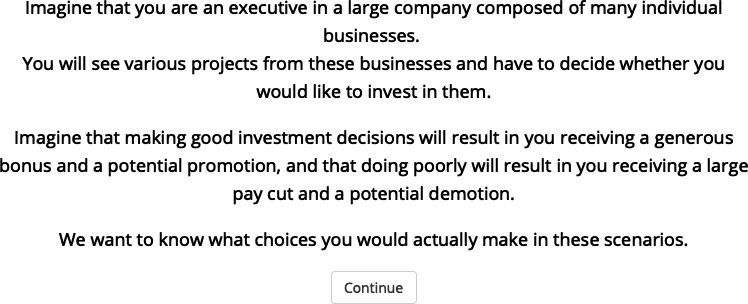
\includegraphics[width=1\linewidth]{thesis_files/figure-latex/instructions-materials-aggregation-1-1} \caption{Experiment 1 instructions. Border added for clarity.}\label{fig:instructions-materials-aggregation-1}
\end{figure}

\paragraph{Outcome distribution decision}

Figure~\ref{fig:project-choice-aggregated-aggregation-1} shows the outcome
distribution display that participants saw in Experiment 1.



\begin{figure}
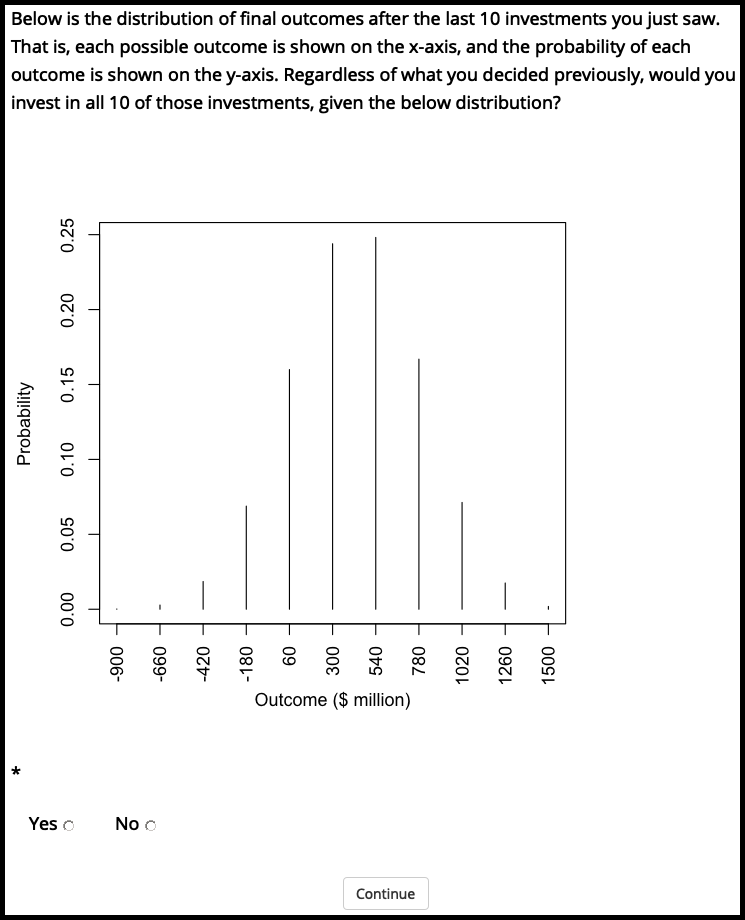
\includegraphics[width=1\linewidth]{thesis_files/figure-latex/project-choice-aggregated-aggregation-1-1} \caption{The outcome distribution of the 10 gambles used in Experiment 1. Border added for clarity.}\label{fig:project-choice-aggregated-aggregation-1}
\end{figure}

\hypertarget{follow-up-materials-aggregation-1-appendix}{%
\paragraph{Follow-up gambles}\label{follow-up-materials-aggregation-1-appendix}}

\subparagraph{Negative EV gambles}

It was important to make sure that participants were generally making decisions
that were in line with EV theory and that the sample was not abnormally risk
tolerant. As such, participants saw two project decisions that had a negative
EV. Out of the 396 negative EV gambles
included (two per participant), all but four
were rejected.

\subparagraph{\texorpdfstring{\textcite{samuelson1963} gambles}{Samuelson (1963) gambles}}

Participants saw the original \textcite{samuelson1963} gamble, were asked whether they
would accept 10 of that gamble, and whether they would accept those 10 given the
associated outcome distribution. They then saw the same three questions, but
using outcome magnitudes that were similar to the ones in the risky investment
task. That is, \$100 million instead of \$100.

\subparagraph{\texorpdfstring{\textcite{redelmeier1992} gambles}{Redelmeier \& Tversky (1992) gambles}}

Participants saw the same three types of gambles (single, 10, and aggregated),
but with the values from the gambles that were used by \textcite{redelmeier1992}.

\hypertarget{results-aggregation-1-appendix}{%
\subsection{Results}\label{results-aggregation-1-appendix}}

\hypertarget{trial-by-trial-aggregation-1}{%
\subsubsection{Trial-by-trial analysis}\label{trial-by-trial-aggregation-1}}

Figure~\ref{fig:plot-aggregation-1-trials} shows proportions of project
acceptance across all conditions and trials.



\begin{figure}
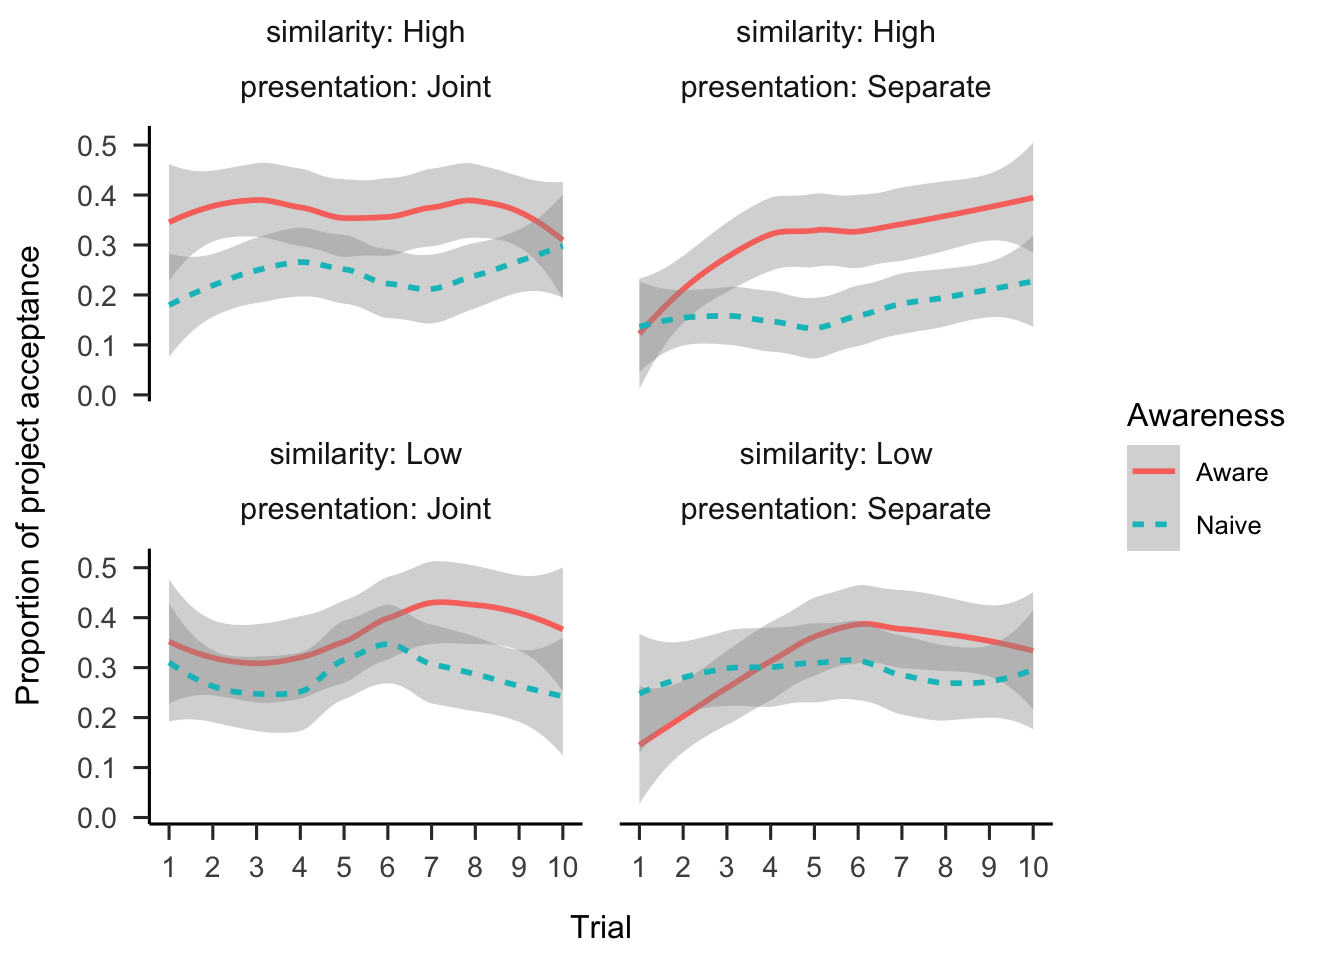
\includegraphics[width=1\linewidth]{thesis_files/figure-latex/plot-aggregation-1-trials-1} \caption{Proportion of project acceptance by trial, similarity, awareness, and presentation conditions. LOESS is used for smoothing over trials, and the shading represents 95\% confidence intervals.}\label{fig:plot-aggregation-1-trials}
\end{figure}

\hypertarget{outcome-distribution-aggregation-1}{%
\subsubsection{Outcome distribution}\label{outcome-distribution-aggregation-1}}

A paired-samples t-test was conducted to compare participants' decision to
invest in the 10 projects while seeing an aggregated distribution, and their
decisions to invest in the projects individually, without the distribution.
Participants invested in the 10 projects more when seeing the distribution both
in the separate presentation phase,
\(t(197) = 5.48\), \(p < .001\), \(d_z = 0.50\), 95\% CI \([0.31, 0.68]\); and in the joint
presentation phase, \(t(197) = 4.17\), \(p < .001\), \(d_z = 0.37\), 95\% CI \([0.19, 0.56]\).

However, it was subsequently discovered that the code that generated this
distribution mistakenly flipped the outcome values. This means that although it
appeared from the distribution that the probability of loss was
0.09, the actual probability of loss of the
underlying values given the correct distribution was
0.26. As such, even though Experiment~1
found an effect of distribution, it was unclear if the effect was driven by
participants actually accurately assessing the riskiness of the individual
gambles, and therefore showing a difference between the isolated and aggregated
gambles in a normative way.

\section{Experiment 2}

\subsection{Method}

\subsubsection{Participants}

\hypertarget{power-analysis-aggregation-2}{%
\paragraph{Power analysis}\label{power-analysis-aggregation-2}}

The power analysis was conducted using the \texttt{pwr} package \autocite{champely2020}, based
on the presentation effect size from Experiment~1, since it was the smallest
effect. The analysis suggested that a minimum sample size of
164 (41 \(\cdot\) 4) was required for
the presentation effect with an expected power of at least 80\%.

\subsubsection{Materials}

\hypertarget{follow-up-materials-aggregation-2-appendix}{%
\paragraph{Follow-up}\label{follow-up-materials-aggregation-2-appendix}}

Figure~\ref{fig:project-number-aggregation-2} shows the project number
question. The maximum value that they could enter was set to 20.
Figures~\ref{fig:portfolio-binary-aggregation-2}
and~\ref{fig:portfolio-number-aggregation-2} ask participants whether they are
willing to take all or none of the projects; and how many projects would they
choose if they could pick randomly (maximum value was set to 20). Those in the
distribution absent condition were asked the same questions, but without the
distribution and its explanation.



\begin{figure}
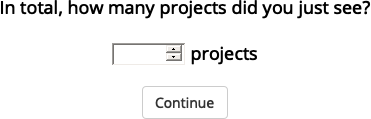
\includegraphics[width=0.5\linewidth]{thesis_files/figure-latex/project-number-aggregation-2-1} \caption{Experiment~2 project number question. Border added for clarity.}\label{fig:project-number-aggregation-2}
\end{figure}



\begin{figure}
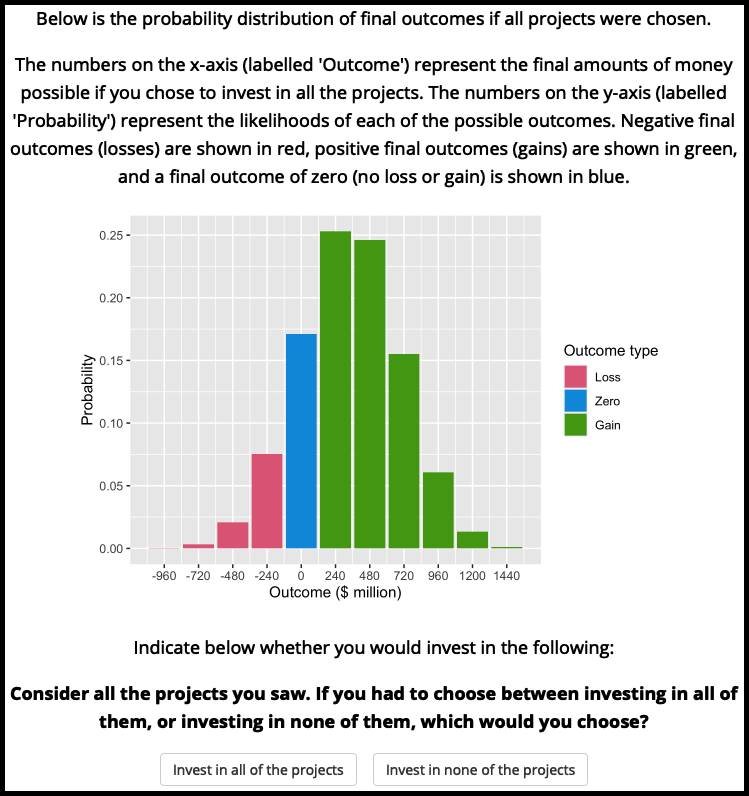
\includegraphics[width=1\linewidth]{thesis_files/figure-latex/portfolio-binary-aggregation-2-1} \caption{Experiment~2 binary portfolio question. Border added for clarity.}\label{fig:portfolio-binary-aggregation-2}
\end{figure}



\begin{figure}
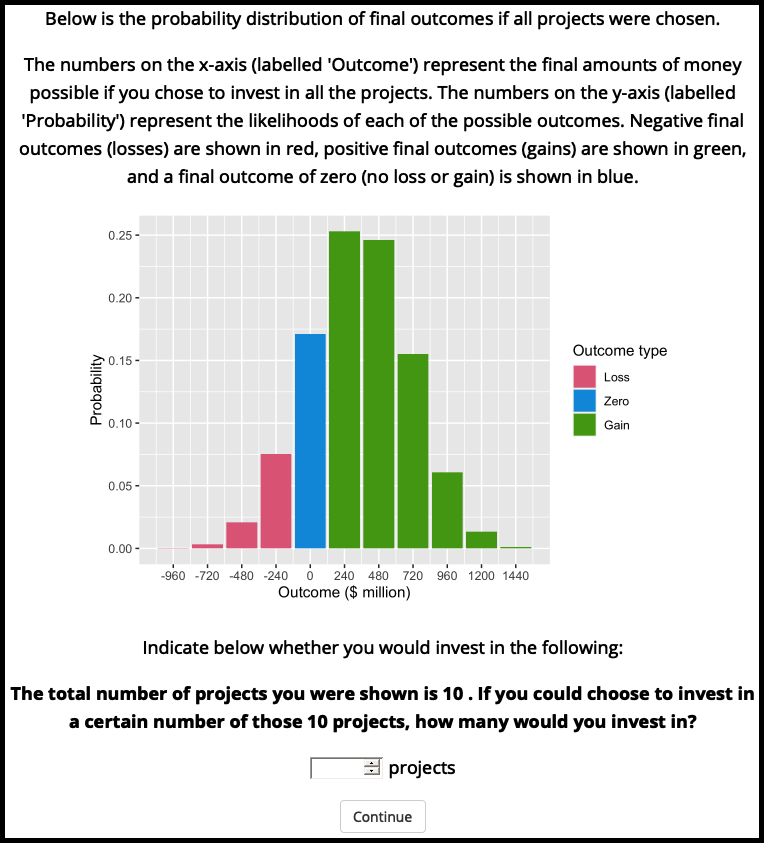
\includegraphics[width=1\linewidth]{thesis_files/figure-latex/portfolio-number-aggregation-2-1} \caption{Experiment~2 numerical portfolio question. Border added for clarity.}\label{fig:portfolio-number-aggregation-2}
\end{figure}

\hypertarget{results-aggregation-2-appendix}{%
\subsection{Results}\label{results-aggregation-2-appendix}}

\subsubsection{Follow-up}

\paragraph{Project number}

Participants were asked how many projects they thought they saw.
Figure~\ref{fig:plot-aggregation-2-project-number} shows that overall people
correctly estimated the number of projects, with more accuracy for those in the
aware condition.



\begin{figure}
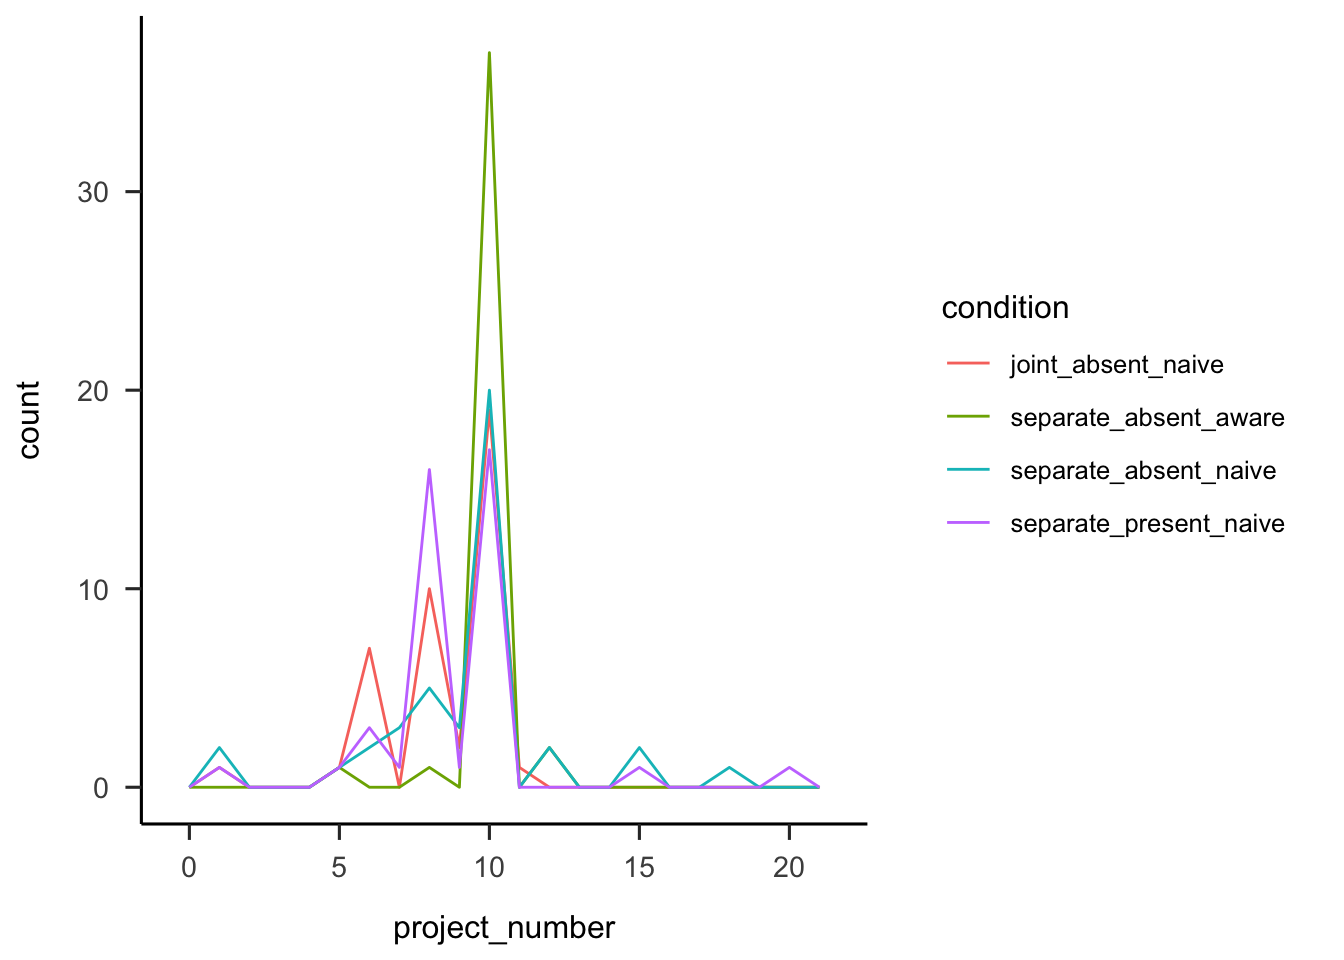
\includegraphics[width=1\linewidth]{thesis_files/figure-latex/plot-aggregation-2-project-number-1} \caption{Number of projects participants reported seeing, by condition.}\label{fig:plot-aggregation-2-project-number}
\end{figure}

\paragraph{Portfolio choice - binary}

Participants were then asked if they would rather invest in all or none of the
projects. As Figure~\ref{fig:plot-aggregation-2-portfolio-binary} shows, the
difference between presentation conditions was not significant,
\(\hat{\beta} = -0.30\), 95\% CI \([-1.19, 0.58]\), \(z = -0.67\), \(p = .500\). The
awareness effect was also not significant,
\(\hat{\beta} = -0.55\), 95\% CI \([-1.44, 0.34]\), \(z = -1.21\), \(p = .225\). However,
those that that saw a distribution chose to invest in all 10 projects
significantly more
(71.43\%) than
those that did not see a distribution
(36.59\%),
\(OR = 4.33\), 95\% CI \([1.76, 11.24]\), \(z = 3.11\), \(p = .002\).



\begin{figure}
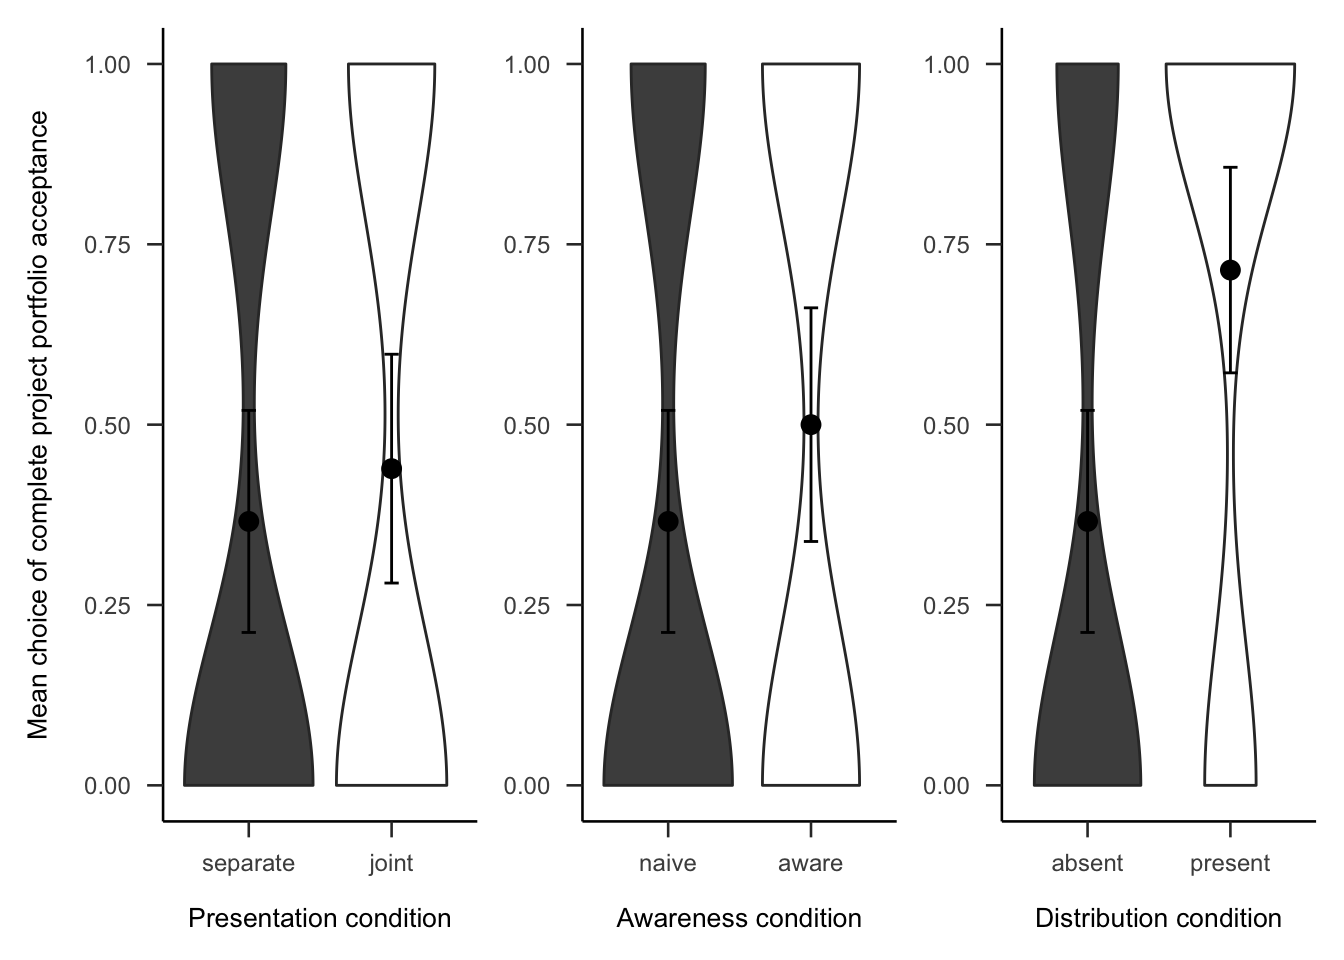
\includegraphics[width=1\linewidth]{thesis_files/figure-latex/plot-aggregation-2-portfolio-binary-1} \caption{Mean choice of investing in all 10 projects for the presentation, awareness, and distribution effects. Note, the condition on the left of each effect is the reference condition (separate presentation, naive awareness, distribution absent). As such, it is identical for the three effects.}\label{fig:plot-aggregation-2-portfolio-binary}
\end{figure}

\paragraph{Portfolio choice - number}

Subsequently, participants were asked how many projects they would invest in out
of the 10 that they saw. As
Figure~\ref{fig:plot-aggregation-2-portfolio-number} shows, the difference
between presentation conditions was not significant,
\(d_s\) = 0.08, 95\% CI {[}-0.35, 0.52{]}, \(t\)(80) = 0.38, \(p\) = .706. The awareness effect
was also not significant, \(d_s\) = 0.09, 95\% CI {[}-0.34, 0.53{]}, \(t\)(79) = 0.42, \(p\) = .678.
However, those that that saw a distribution chose to invest in significantly
more projects than those that did not see a distribution,
\(d_s\) = 0.60, 95\% CI {[}0.15, 1.03{]}, \(t\)(81) = 2.70, \(p\) = .009.



\begin{figure}
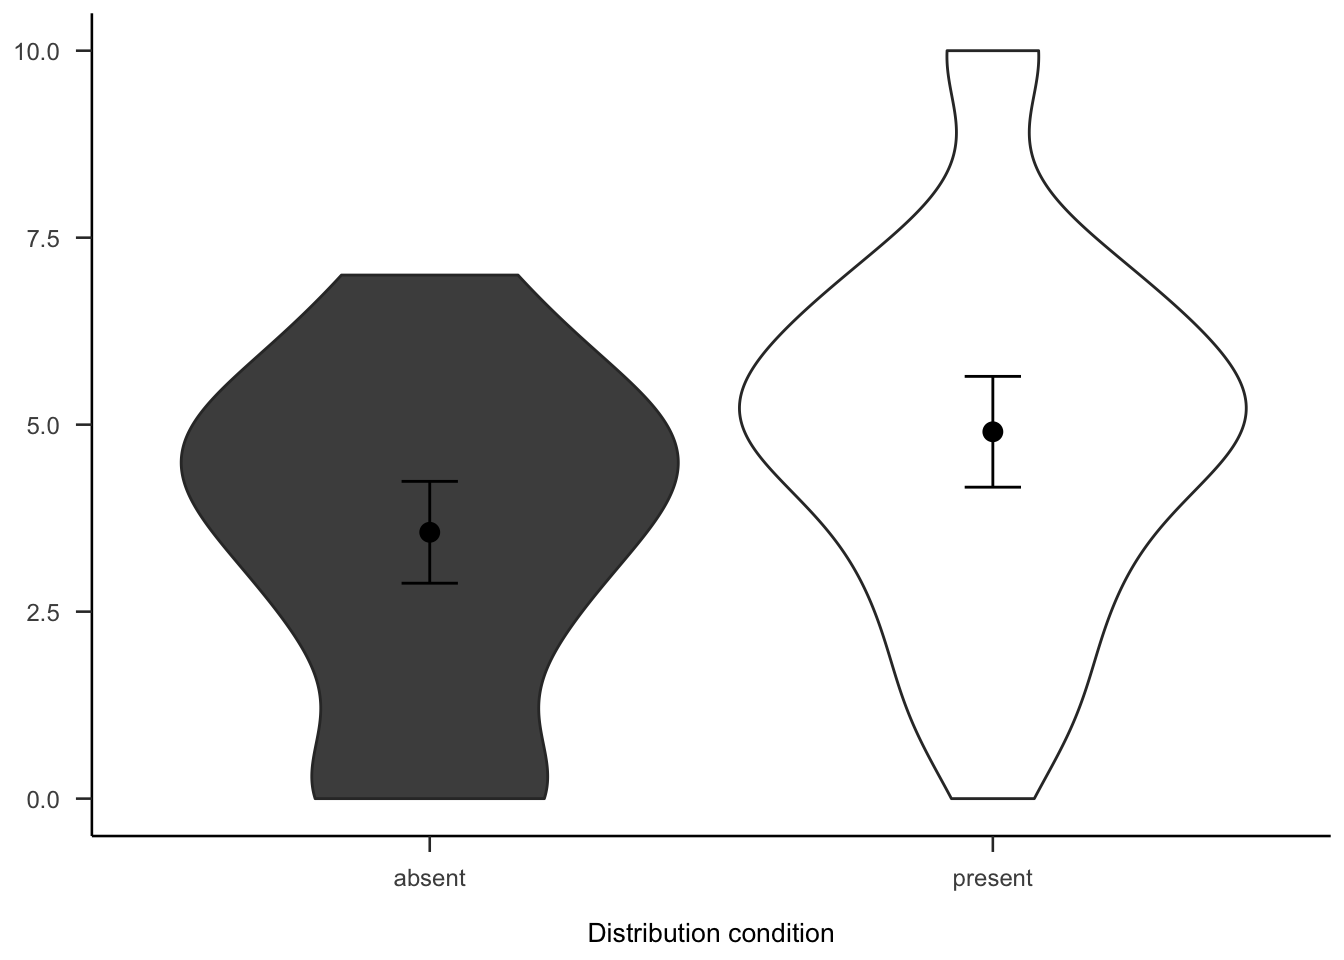
\includegraphics[width=1\linewidth]{thesis_files/figure-latex/plot-aggregation-2-portfolio-number-1} \caption{Mean number of projects chosen in the follow-up for the presentation, awareness, and distribution effects. Note, the condition on the left of each effect is the reference condition (separate presentation, naive awareness, distribution absent). As such, it is identical for the three effects.}\label{fig:plot-aggregation-2-portfolio-number}
\end{figure}

\subsubsection{Gambles}

Figures~\ref{fig:plot-aggregation-2-trials}
and~\ref{fig:plot-aggregation-2-gamble-values} show that the overall people
seemed to prefer gambles with higher probabilities of gain, sometimes regardless
of expected value or value of the gain.



\begin{figure}
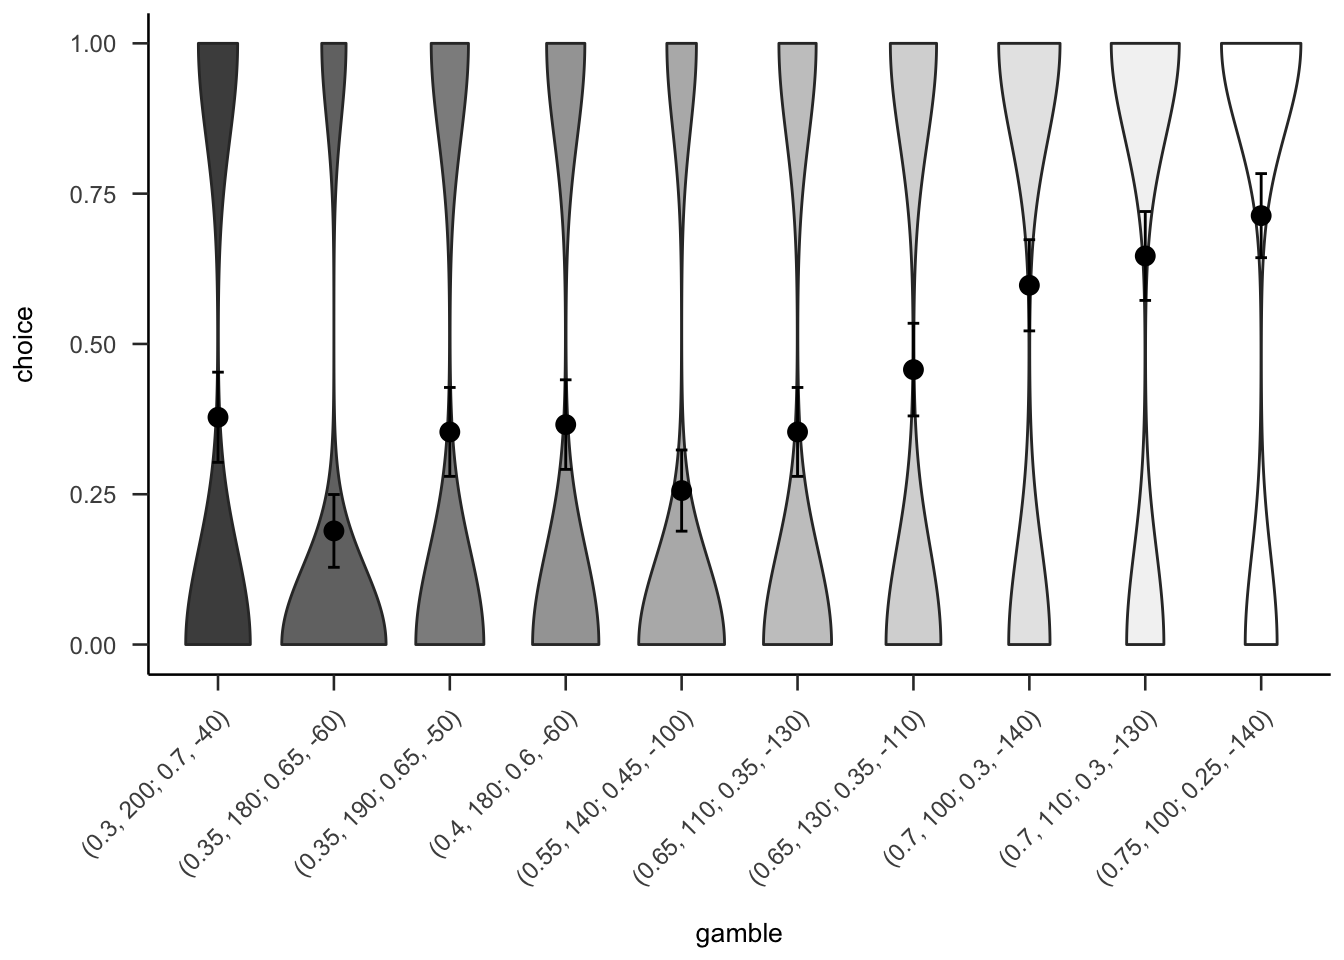
\includegraphics[width=1\linewidth]{thesis_files/figure-latex/plot-aggregation-2-trials-1} \caption{Mean project acceptance for the 10 gambles. The format of the labels indicates: (gain probability, gain value; loss probability, loss value).}\label{fig:plot-aggregation-2-trials}
\end{figure}



\begin{figure}
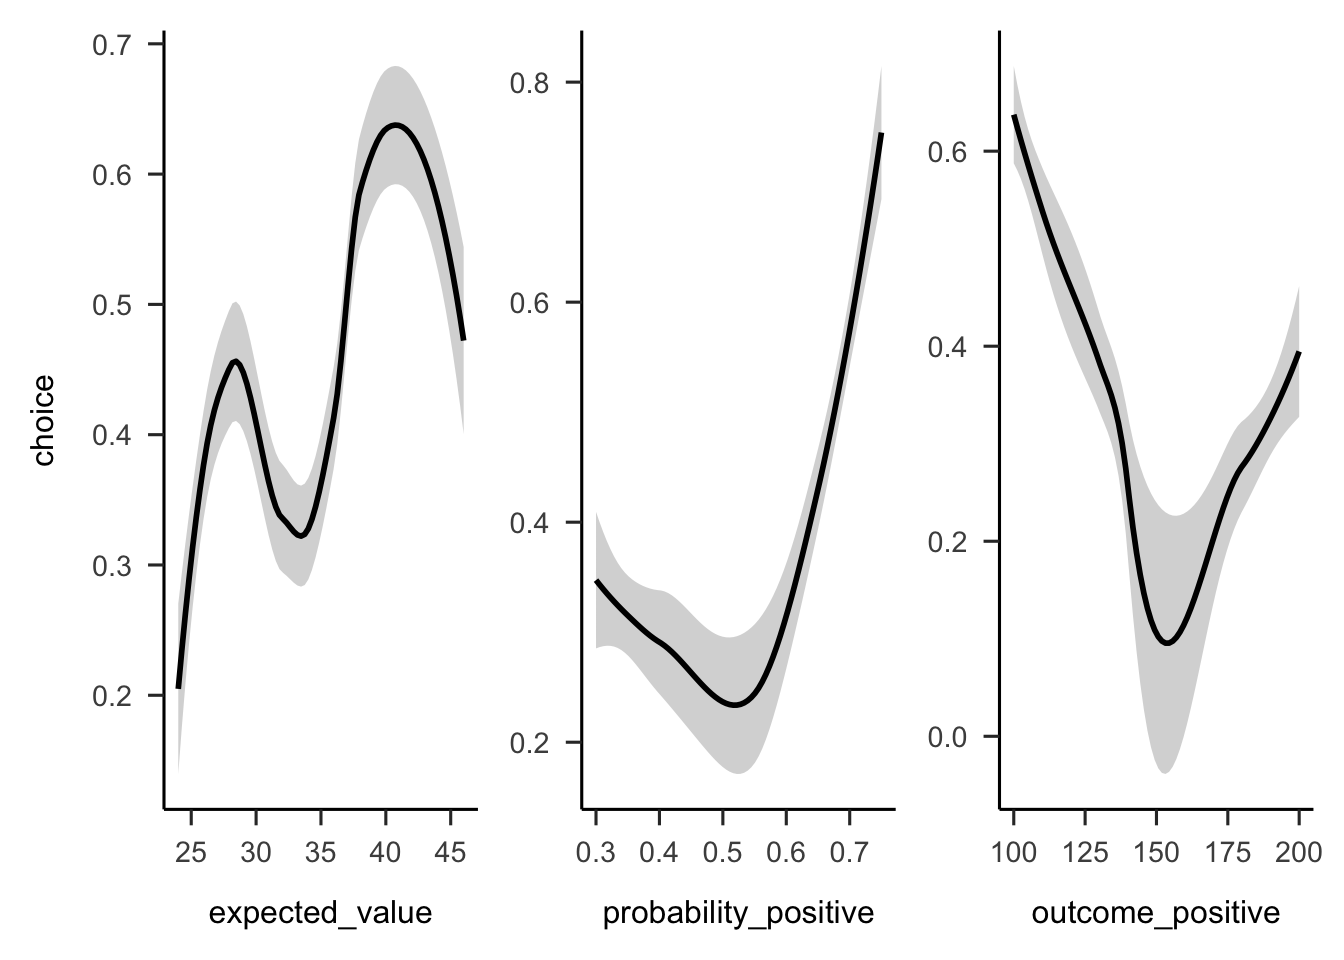
\includegraphics[width=1\linewidth]{thesis_files/figure-latex/plot-aggregation-2-gamble-values-1} \caption{Mean project acceptance for the gambles' expected value, positive probability, and positive outcome.}\label{fig:plot-aggregation-2-gamble-values}
\end{figure}

\hypertarget{aggregation-3}{%
\section{Experiment~3}\label{aggregation-3}}

Experiment~3 investigated the effect of similarity on project choice. The
previous experiments did not counterbalance the project domain when displaying
the 10 projects to participants. Experiment~3 used 10 different potential
business domains when constructing the project descriptions in order to reduce
any potential effect that the specific domain may have on people's choice.
Therefore, Experiment~3 again tested
Hypothesis~\ref{hyp:similarity-aggregation-1}.

\subsection{Method}

\subsubsection{Participants}

Two hundred and sixty-six people (127 female) were recruited from the online recruitment platform Prolific. Participants were compensated at a rate of £5 an hour. The average age was 39.56 (\emph{SD} = 8.77, \emph{min} = 25, \emph{max} = 71). Participants reported an average of 5.64 (\emph{SD} = 6.45, \emph{min} = 0, \emph{max} = 40) years of work in a business setting, and an average of 3.28 (\emph{SD} = 4.92, \emph{min} = 0, \emph{max} = 30) years of business education. The mean completion time was 9.23 (\emph{SD} = 7.2, \emph{min} = 1.41, \emph{max} = 65.46) minutes.~Table~\ref{tab:condition-allocation-aggregation-3}
shows the between-subjects condition allocation.

\begin{table}[tbp]

\begin{center}
\begin{threeparttable}

\caption{\label{tab:condition-allocation-aggregation-3}Experiment 3 group allocation.}

\begin{tabular}{ll}
\toprule
Similarity & \multicolumn{1}{c}{N}\\
\midrule
High & 133\\
Low & 133\\
Total & 266\\
\bottomrule
\end{tabular}

\end{threeparttable}
\end{center}

\end{table}

\subsubsection{Materials}

\paragraph{Instructions}

Participants were shown the same instructions as in Experiment~1 (see
Section~\ref{instructions-materials-aggregation-1}).

\hypertarget{task-aggregation-3}{%
\paragraph{Risky investment task}\label{task-aggregation-3}}

Participants saw displays with the same gamble values as those in Experiment~2
(see Section~\ref{task-aggregation-2}), but with some changes in wording and
sentence structure. The gamble information was the same, but extra prose was
added to describe the projects. Further, the order of the sentences was
randomised, so that the descriptions would not appear so similar. See
Figure~\ref{fig:project-choice-aggregation-3} for an example.



\begin{figure}
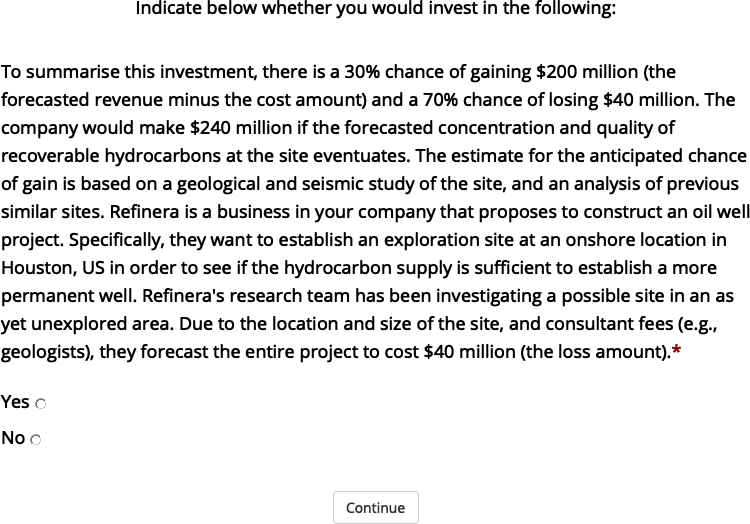
\includegraphics[width=1\linewidth]{thesis_files/figure-latex/project-choice-aggregation-3-1} \caption{An example of a project display in Experiment~3. Border added for clarity.}\label{fig:project-choice-aggregation-3}
\end{figure}

The similarity manipulation was as in Experiment~1. However, project domain was
varied so that in the high similarity condition participants saw one of ten
project domains.

\hypertarget{follow-up-aggregation-3}{%
\paragraph{Follow-up}\label{follow-up-aggregation-3}}

The follow-up questions were similar to those in Experiment~2 (see
Section~\ref{follow-up-aggregation-2}), except in the portfolio number question
participants were also shown the total number of projects that they saw (10).
Further, another question was added, asking how many projects participants were
expecting to see at the beginning of the experiment (see
Figure~\ref{fig:project-expectation-aggregation-3}).



\begin{figure}

\includegraphics[width=1\linewidth]{thesis_files/figure-latex/project-expectation-aggregation-3-1} \caption{Experiment~3 project expectation question. Border added for clarity.}\label{fig:project-expectation-aggregation-3}
\end{figure}

\subsubsection{Procedure}

Participants read the instructions and completed the risky investment task in
their respective conditions. After seeing the individual projects, participants
were then asked the four follow-up questions.

\subsection{Results}

\subsubsection{Project investment}

The project investment data were analysed as in Experiment~2 (see
Section~\ref{results-aggregation-2}).
Figures~\ref{fig:plot-aggregation-3-choice}
and~\ref{fig:plot-aggregation-3-proportion} show the choice and proportion
data, respectively. The difference between similarity conditions was not
significant, both in the logistic regression
\(b = 0.00\), 95\% CI \([-0.18, 0.17]\), \(z = -0.04\), \(p = .966\), and in the t-test,
\(d_s\) = -0.21, 95\% CI {[}-0.45, 0.03{]}, \(t\)(264) = -1.69, \(p\) = .093.



\begin{figure}
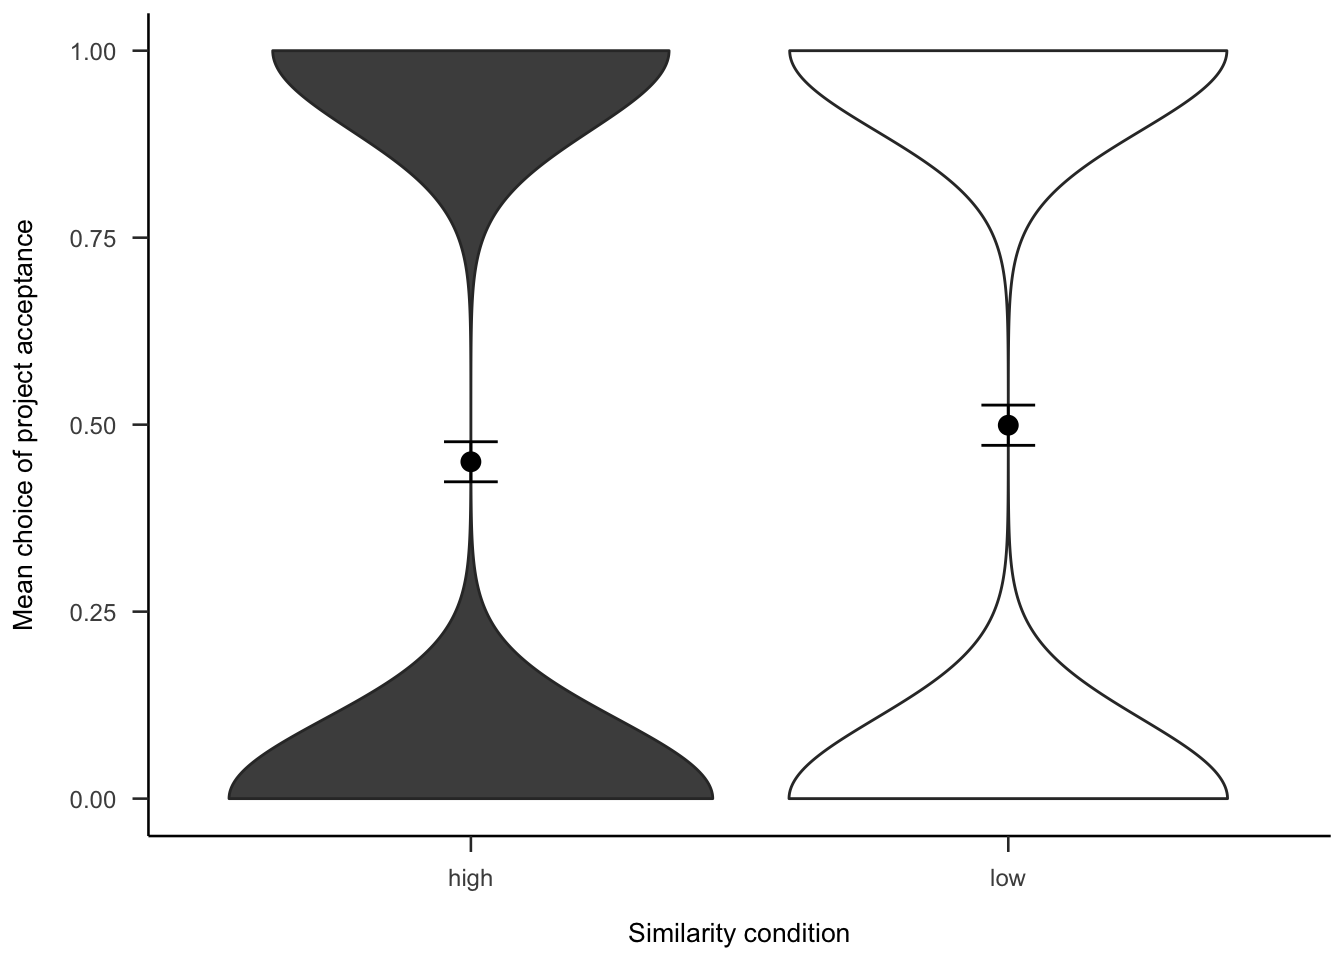
\includegraphics[width=1\linewidth]{thesis_files/figure-latex/plot-aggregation-3-choice-1} \caption{Mean project acceptance for the similarity effect.}\label{fig:plot-aggregation-3-choice}
\end{figure}



\begin{figure}
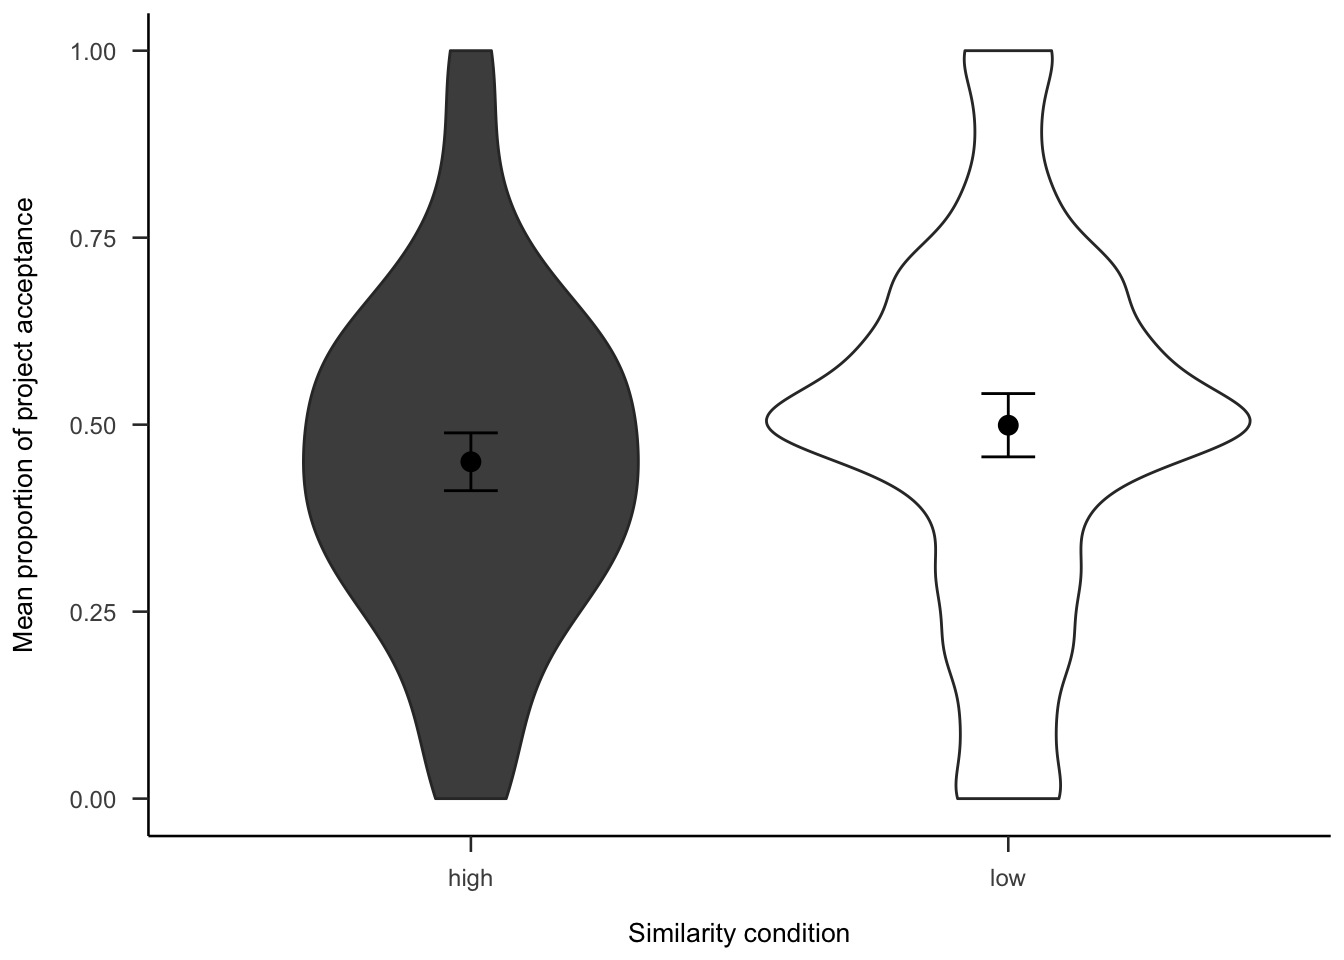
\includegraphics[width=1\linewidth]{thesis_files/figure-latex/plot-aggregation-3-proportion-1} \caption{Mean proportion of project acceptance for the similarity effect.}\label{fig:plot-aggregation-3-proportion}
\end{figure}

Further, Figure~\ref{fig:plot-aggregation-3-choice-trials} shows the choice
data as a function of the order of the project in the sequence. As
Table~\ref{tab:similarity-project-order} shows, there were no main effects or
interactions.



\begin{figure}
\includegraphics[width=1\linewidth]{thesis_files/figure-latex/plot-aggregation-3-choice-trials-1} \caption{Mean project acceptance by similarity and trial.}\label{fig:plot-aggregation-3-choice-trials}
\end{figure}

\begin{table}[tbp]

\begin{center}
\begin{threeparttable}

\caption{\label{tab:similarity-project-order}Logistic regression table of project acceptance by similarity and trial.}

\begin{tabular}{lllll}
\toprule
Term & \multicolumn{1}{c}{$\hat{\beta}$} & \multicolumn{1}{c}{95\% CI} & \multicolumn{1}{c}{$z$} & \multicolumn{1}{c}{$p$}\\
\midrule
Intercept & 0.01 & {}[-0.20, 0.22] & 0.07 & .944\\
Similarity1 & -0.02 & {}[-0.23, 0.18] & -0.22 & .826\\
Project order & -0.02 & {}[-0.05, 0.01] & -1.52 & .127\\
Similarity1 $\times$ Project order & -0.02 & {}[-0.05, 0.01] & -1.07 & .284\\
\bottomrule
\end{tabular}

\end{threeparttable}
\end{center}

\end{table}

\subsubsection{Follow-up}

\paragraph{Project expectation}

Participants were asked how many projects they expected to see. As
Figure~\ref{fig:plot-aggregation-3-project-expectation} shows, the difference
between similarity conditions was not significant,
\(d_s\) = -0.23, 95\% CI {[}-0.47, 0.01{]}, \(t\)(264) = -1.85, \(p\) = .065.



\begin{figure}
\includegraphics[width=1\linewidth]{thesis_files/figure-latex/plot-aggregation-3-project-expectation-1} \caption{Number of projects participants expected to see, by similarity.}\label{fig:plot-aggregation-3-project-expectation}
\end{figure}

\paragraph{Project number}

Participants were asked how many projects they thought they saw.
Figure~\ref{fig:plot-aggregation-3-project-number} shows that overall people
correctly estimate the number of projects.



\begin{figure}
\includegraphics[width=1\linewidth]{thesis_files/figure-latex/plot-aggregation-3-project-number-1} \caption{Number of projects participants reported seeing, by similarity.}\label{fig:plot-aggregation-3-project-number}
\end{figure}

\paragraph{Portfolio choice - binary}

Participants were then asked if they would rather invest in all or none of the
projects. As Figure~\ref{fig:plot-aggregation-3-portfolio-binary} shows, those
in the low similarity condition were significantly more likely to want to invest
in all of the projects,
\(b = -0.26\), 95\% CI \([-0.51, -0.02]\), \(z = -2.10\), \(p = .036\).



\begin{figure}
\includegraphics[width=1\linewidth]{thesis_files/figure-latex/plot-aggregation-3-portfolio-binary-1} \caption{Mean choice of investing in all 10 projects for the similarity effect.}\label{fig:plot-aggregation-3-portfolio-binary}
\end{figure}

\paragraph{Portfolio choice - number}

Subsequently, participants were asked how many projects they would invest in out
of the 10 that they saw. As
Figure~\ref{fig:plot-aggregation-3-portfolio-number} shows, the difference
between similarity conditions was not significant,
\(d_s\) = -0.14, 95\% CI {[}-0.38, 0.10{]}, \(t\)(264) = -1.12, \(p\) = .264.



\begin{figure}
\includegraphics[width=1\linewidth]{thesis_files/figure-latex/plot-aggregation-3-portfolio-number-1} \caption{Mean number of projects chosen in the follow-up for the similarity effect.}\label{fig:plot-aggregation-3-portfolio-number}
\end{figure}

\subsubsection{Gambles}

Figures~\ref{fig:plot-aggregation-3-trials}
and~\ref{fig:plot-aggregation-3-gamble-values} show the
overall people seemed to prefer gambles with higher probabilities of gain,
sometimes regardless of expected value or value of the gain.



\begin{figure}
\includegraphics[width=1\linewidth]{thesis_files/figure-latex/plot-aggregation-3-trials-1} \caption{Mean project acceptance for the 10 gambles. The format of the labels indicate: (gain probability, gain value; loss probability, loss value).}\label{fig:plot-aggregation-3-trials}
\end{figure}




\begin{figure}
\includegraphics[width=1\linewidth]{thesis_files/figure-latex/plot-aggregation-3-gamble-values-1} \caption{Mean project acceptance for the gambles'
expected value, positive probability, and positive outcome.}\label{fig:plot-aggregation-3-gamble-values}
\end{figure}

\subsection{Discussion}

Experiment~3 found some evidence for the effect of similarity on project choice,
but it was in the opposite direction to the one hypothesised. Specifically, the
results showed that when considering projects individually, participants' risk
aversion did not differ between similarity conditions, but when offered a
portfolio of the projects, those that saw the dissimilar projects were more
likely to invest.

These results provide evidence for the naive diversification account expressed
above (see Section~\ref{similarity-discussion-aggregation-1}). Specifically,
participants may really be naively diversifying, but only when they are
explicitly given an opportunity to do so. This is similar to the multi-play
effects because the question itself provides a sort of choice bracketing. That
is, the gambles are grouped together as a portfolio by the question. Together,
this suggests that people are not naively aggregating when viewing gambles in
isolation, but when the choices are bracketed explicitly, then the choice seems
to be driven by a naive diversification.

\hypertarget{aggregation-4}{%
\section{Experiment 4}\label{aggregation-4}}

Experiment~4 investigated the effect of awareness on project choice.
Experiment~1 found an effect of awareness in the trial-by-trial data that was
not replicated in Experiment~2. Above, this effect was explained through the law
of small numbers: people may have been anticipating less risky gambles towards
the end of the set. As such, the effect could be seen with more trials.
Experiment~4 attempted to replicate the effect from Experiment~1 with 20
projects. The \emph{naive} condition attempted to encourage participants to focus on
projects one at a time and did not reveal the total number of projects. The
\emph{aware} condition attempted to encourage participants to think of all 20
projects. This was done by revealing the total number of projects in the
beginning of the task and by identifying at each project display its order in
the sequence. Experiment~4 again tested
Hypothesis~\ref{hyp:awareness-trials-aggregation-2}.

\subsection{Method}

\subsubsection{Participants}

Two hundred and sixty-six people (110 female) were recruited from the online recruitment platform Prolific. Participants were compensated at a rate of £5 an hour. The average age was 40.62 (\emph{SD} = 9.59, \emph{min} = 25, \emph{max} = 74). Participants reported an average of 7.45 (\emph{SD} = 7.8, \emph{min} = 0, \emph{max} = 47) years of work in a business setting, and an average of 5.52 (\emph{SD} = 7.27, \emph{min} = 0, \emph{max} = 48) years of business education. The mean completion time was 12.66 (\emph{SD} = 8.26, \emph{min} = 1.48, \emph{max} = 53.47) minutes.~Table~\ref{tab:condition-allocation-aggregation-4}
shows the between-subjects condition allocation.

\begin{table}[tbp]

\begin{center}
\begin{threeparttable}

\caption{\label{tab:condition-allocation-aggregation-4}Experiment 4 group allocation.}

\begin{tabular}{ll}
\toprule
Awareness & \multicolumn{1}{c}{N}\\
\midrule
Aware & 133\\
Naive & 133\\
Total & 266\\
\bottomrule
\end{tabular}

\end{threeparttable}
\end{center}

\end{table}

\subsubsection{Materials}

\paragraph{Instructions}

Participants were shown similar instructions to Experiment~1 (see
Section~\ref{instructions-materials-aggregation-1}), except that the awareness
manipulation was incorporated into the text. Participants in the naive condition
saw the instructions in Figure~\ref{fig:instructions-naive-aggregation-4}, and
those in the aware condition saw the instructions in
Figure~\ref{fig:instructions-aware-aggregation-4}.



\begin{figure}
\includegraphics[width=1\linewidth]{thesis_files/figure-latex/instructions-naive-aggregation-4-1} \caption{Instructions for those in the naive condition of Experiment~4. Border added for clarity.}\label{fig:instructions-naive-aggregation-4}
\end{figure}



\begin{figure}
\includegraphics[width=1\linewidth]{thesis_files/figure-latex/instructions-aware-aggregation-4-1} \caption{Instructions for those in the aware condition of Experiment~4. Border added for clarity.}\label{fig:instructions-aware-aggregation-4}
\end{figure}

\paragraph{Risky investment task}

Participants saw similar displays to those in Experiment~3 (see
Section~\ref{task-aggregation-3}). However, here participants viewed 20
projects, so while the gamble constrains explained above were still applied, the
actual gamble values were different. Further, those in the aware condition saw
an added sentence that identified the number of the project they were currently
considering in the context of the total 20. See
Figure~\ref{fig:project-choice-aggregation-4} for an example. Those in the
naive condition saw the same display without this sentence.



\begin{figure}
\includegraphics[width=1\linewidth]{thesis_files/figure-latex/project-choice-aggregation-4-1} \caption{An example of a project display in Experiment~4. Border added for clarity.}\label{fig:project-choice-aggregation-4}
\end{figure}

\paragraph{Follow-up}

The follow-up questions were identical to those in Experiment~3 (see
Section~\ref{follow-up-aggregation-3}), except that the portfolio number
question identified the number of projects they saw as 20.

\subsubsection{Procedure}

Participants read the instructions and completed the risky investment task in
their respective conditions. After seeing the individual projects, participants
were then asked the four follow-up questions.

\subsection{Results}

\subsubsection{Project investment}

The project investment data were analysed as in Experiment~2 (see
Section~\ref{results-aggregation-2}).
Figures~\ref{fig:plot-aggregation-4-choice}
and~\ref{fig:plot-aggregation-4-proportion} show the choice and proportion
data, respectively. The difference between awareness conditions was not
significant, both in the logistic regression
\(b = -0.05\), 95\% CI \([-0.22, 0.13]\), \(z = -0.53\), \(p = .595\), and in the t-test,
\(d_s\) = -0.09, 95\% CI {[}-0.33, 0.15{]}, \(t\)(264) = -0.73, \(p\) = .464.



\begin{figure}
\includegraphics[width=1\linewidth]{thesis_files/figure-latex/plot-aggregation-4-choice-1} \caption{Mean project acceptance for the awareness effect.}\label{fig:plot-aggregation-4-choice}
\end{figure}



\begin{figure}
\includegraphics[width=1\linewidth]{thesis_files/figure-latex/plot-aggregation-4-proportion-1} \caption{Mean proportion of project acceptance for the awareness effect.}\label{fig:plot-aggregation-4-proportion}
\end{figure}

Further, Figure~\ref{fig:plot-aggregation-4-choice-trials} shows the choice
data as a function of the order of the project in the sequence. As
Table~\ref{tab:awareness-project-order} shows, there were no main effects or
interactions.



\begin{figure}
\includegraphics[width=1\linewidth]{thesis_files/figure-latex/plot-aggregation-4-choice-trials-1} \caption{Mean project acceptance by awareness and trial.}\label{fig:plot-aggregation-4-choice-trials}
\end{figure}

\begin{table}[tbp]

\begin{center}
\begin{threeparttable}

\caption{\label{tab:awareness-project-order}Logistic regression table of project acceptance by awareness and trial.}

\begin{tabular}{lllll}
\toprule
Term & \multicolumn{1}{c}{$\hat{\beta}$} & \multicolumn{1}{c}{95\% CI} & \multicolumn{1}{c}{$z$} & \multicolumn{1}{c}{$p$}\\
\midrule
Intercept & -0.01 & {}[-0.20, 0.17] & -0.12 & .907\\
Awareness1 & -0.10 & {}[-0.28, 0.09] & -1.05 & .293\\
Project order & 0.01 & {}[0.00, 0.02] & 1.66 & .096\\
Awareness1 $\times$ Project order & 0.00 & {}[-0.01, 0.01] & 0.29 & .775\\
\bottomrule
\end{tabular}

\end{threeparttable}
\end{center}

\end{table}

\subsubsection{Follow-up}

\paragraph{Project expectation}

Participants were asked how many projects they expected to see.
Figure~\ref{fig:plot-aggregation-4-project-expectation} shows that those in the
aware condition reportedly expect to see more,
\(d_s\) = -0.94, 95\% CI {[}-1.19, -0.69{]}, \(t\)(264) = -7.67, \(p\) \textless{} .001. However, this is likely to be due to
the fact that they were told how many projects there were.



\begin{figure}
\includegraphics[width=1\linewidth]{thesis_files/figure-latex/plot-aggregation-4-project-expectation-1} \caption{Number of projects participants expected to see, by awareness.}\label{fig:plot-aggregation-4-project-expectation}
\end{figure}

\paragraph{Project number}

Participants were asked how many projects they thought they saw.
Figure~\ref{fig:plot-aggregation-4-project-number} shows that overall people
correctly estimated the number of projects, with higher accuracy for those in the
aware condition.



\begin{figure}
\includegraphics[width=1\linewidth]{thesis_files/figure-latex/plot-aggregation-4-project-number-1} \caption{Number of projects participants reported seeing, by awareness.}\label{fig:plot-aggregation-4-project-number}
\end{figure}

\paragraph{Portfolio choice - binary}

Participants were then asked if they would rather invest in all or none of the
projects. As Figure~\ref{fig:plot-aggregation-4-portfolio-binary}, there was no
significant difference between awareness conditions in wanting to invest
in all of the projects,
\(b = -0.09\), 95\% CI \([-0.33, 0.15]\), \(z = -0.74\), \(p = .460\).



\begin{figure}
\includegraphics[width=1\linewidth]{thesis_files/figure-latex/plot-aggregation-4-portfolio-binary-1} \caption{Mean choice of investing in all 20 projects for the awareness effect.}\label{fig:plot-aggregation-4-portfolio-binary}
\end{figure}

\paragraph{Portfolio choice - number}

Subsequently, we asked participants how many projects they would invest in out
of the 20 that they saw. As
Figure~\ref{fig:plot-aggregation-4-portfolio-number} shows, the difference
between awareness conditions was not significant,
\(d_s\) = -0.12, 95\% CI {[}-0.36, 0.12{]}, \(t\)(264) = -0.97, \(p\) = .334.



\begin{figure}
\includegraphics[width=1\linewidth]{thesis_files/figure-latex/plot-aggregation-4-portfolio-number-1} \caption{Mean number of projects chosen in the follow-up for the awareness effect.}\label{fig:plot-aggregation-4-portfolio-number}
\end{figure}

\subsubsection{Gambles}

Figures~\ref{fig:plot-aggregation-4-trials}
and~\ref{fig:plot-aggregation-4-gamble-values} show the
overall people seemed to prefer gambles with higher probabilities of gain,
sometimes regardless of expected value or value of the gain.



\begin{figure}
\includegraphics[width=1\linewidth]{thesis_files/figure-latex/plot-aggregation-4-trials-1} \caption{Mean project acceptance for the 20 gambles. The format of the labels indicate: (gain probability, gain value; loss probability, loss value).}\label{fig:plot-aggregation-4-trials}
\end{figure}



\begin{figure}
\includegraphics[width=1\linewidth]{thesis_files/figure-latex/plot-aggregation-4-gamble-values-1} \caption{Mean project acceptance for the gambles' expected value, positive probability, and positive outcome.}\label{fig:plot-aggregation-4-gamble-values}
\end{figure}

\subsection{Discussion}

Experiment~4 did not find evidence for
Hypothesis~\ref{hyp:awareness-trials-aggregation-2}. There was no significant
effect of awareness on project choice by trial. Participants in the aware
condition were expected to become less risk averse as they continued with the
experiment if they were using a strategy similar to the law of small numbers.
The fact that this effect was not replicated in Experiment~4 might mean that the
finding in Experiment~1 was due to the specific gambles used in that experiment,
or statistical chance.

\hypertarget{alignment-appendix}{%
\chapter{Chapter~\ref{alignment} appendix}\label{alignment-appendix}}

\minitoc

This appendix contains supplementary materials and analyses for the three
experiments reported in Chapter~\ref{alignment}. In addition, five related
experiments are reported. Experiment~4 was identical to Experiment~1, except
that alignment was manipulated within-subjects, it did not include a no NPV
condition, and there was no forecasting measure. Experiment~5 replicated
Experiment~1, but only tested the forecasting effect and did so with a sample
that had investing experience. Experiment~6 replicated Experiment~5 but with a
larger sample size and a lay sample. Experiment~7 attempted to facilitate a use
of numerical reliability through explicit hints. Experiment~8 tested both verbal
and numerical reliability effects in an all within-subjects design. However,
unlike Experiment~3, the design of Experiment~8 did not allow for a direct
comparison of alignment conditions.

\hypertarget{alignment-2-appendix}{%
\section{Experiment 1}\label{alignment-2-appendix}}

In addition to the allocation measure, participants were also asked to rank the
projects and forecast their future returns. The ranking task was included before
the allocation task in order to encourage alignment and to have another measure
of participants' decision-making. The forecasting task was added (described
further below in Section~\ref{forecasting-materials-alignment-2}) in order to
test whether the variance in people's forecasts is affected by alignment and NPV
reliability.

\begin{hypothesis}
\protect\hypertarget{hyp:ranking-all-alignment-2}{}{\label{hyp:ranking-all-alignment-2} }All allocation effects will replicate in the ranking measure.
\end{hypothesis}

\begin{hypothesis}
\protect\hypertarget{hyp:forecasting-mean-all-alignment-2}{}{\label{hyp:forecasting-mean-all-alignment-2} }All allocation effects will replicate in the forecasting mean measure.
\end{hypothesis}

In the forecasting measures, more alignable differences were expected to bring
about more certainty about forecasting decisions, since participants will have
more easily comparable information. As such, people's forecasting should be less
variable when comparing projects with alignable differences, than when comparing
projects with non-alignable differences.

\begin{hypothesis}
\protect\hypertarget{hyp:forecasting-sd-alignment-alignment-2}{}{\label{hyp:forecasting-sd-alignment-alignment-2} }The standard deviation of participants' forecasts will be higher, on average,
in the low alignment condition than in the high alignment condition.
\end{hypothesis}

\subsection{Method}

\hypertarget{materials-alignment-2-appendix}{%
\subsubsection{Materials}\label{materials-alignment-2-appendix}}

\hypertarget{instructions-materials-alignment-2-appendix}{%
\paragraph{Instructions}\label{instructions-materials-alignment-2-appendix}}

Figures~\ref{fig:instructions-reliability-low-alignment-2},~\ref{fig:instructions-reliability-high-alignment-2},
and~\ref{fig:instructions-reliability-no-npv-alignment-2} show the instructions
given to those in the low NPV reliability, high NPV reliability, and no NPV
condition, respectively.



\begin{figure}
\includegraphics[width=1\linewidth]{thesis_files/figure-latex/instructions-reliability-low-alignment-2-1} \caption{Experiment~1 low reliability instructions. Border added for clarity.}\label{fig:instructions-reliability-low-alignment-2}
\end{figure}



\begin{figure}
\includegraphics[width=1\linewidth]{thesis_files/figure-latex/instructions-reliability-high-alignment-2-1} \caption{Experiment~1 high reliability instructions. Border added for clarity.}\label{fig:instructions-reliability-high-alignment-2}
\end{figure}



\begin{figure}
\includegraphics[width=1\linewidth]{thesis_files/figure-latex/instructions-reliability-no-npv-alignment-2-1} \caption{The instructions for the no NPV condition in Experiment~1. Border added for clarity.}\label{fig:instructions-reliability-no-npv-alignment-2}
\end{figure}

\hypertarget{forecasting-materials-alignment-2}{%
\paragraph{Forecasting}\label{forecasting-materials-alignment-2}}

Participants were asked to respond to a forecasting task \autocite[adapted from][]{long2018}, seen in Figure~\ref{fig:forecasting-materials-alignment-2}.
Participants were asked to predict each project's rate of return after one
month. This allowed to calculate each participant's forecasting mean and
standard deviation (the latter as inversely proportional to forecasting
precision).



\begin{figure}
\includegraphics[width=1\linewidth]{thesis_files/figure-latex/forecasting-materials-alignment-2-1} \caption{The forecasting task. Border added for clarity.}\label{fig:forecasting-materials-alignment-2}
\end{figure}

\hypertarget{ranking-materials-alignment-2}{%
\paragraph{Ranking}\label{ranking-materials-alignment-2}}

As seen in Figure~\ref{fig:ranking-materials-alignment-2}, participants were
asked to rank the projects in order of investment priority.



\begin{figure}
\includegraphics[width=1\linewidth]{thesis_files/figure-latex/ranking-materials-alignment-2-1} \caption{The ranking task. Border added for clarity.}\label{fig:ranking-materials-alignment-2}
\end{figure}

\hypertarget{confidence-materials-alignment-2}{%
\paragraph{Confidence}\label{confidence-materials-alignment-2}}

As Figure~\ref{fig:confidence-materials-alignment-2} shows, participants were
asked to indicate how confident they were about each of their allocation
decisions on a scale from 0 (``Not confident at all'') to 100 (``Extremely
confident'').



\begin{figure}
\includegraphics[width=1\linewidth]{thesis_files/figure-latex/confidence-materials-alignment-2-1} \caption{The confidence task. Border added for clarity.}\label{fig:confidence-materials-alignment-2}
\end{figure}

\hypertarget{justification-materials-alignment-2}{%
\paragraph{Justification}\label{justification-materials-alignment-2}}

As Figure~\ref{fig:justification-materials-alignment-2} shows, participants
were asked to justify their allocation decision in a free-response text-box.



\begin{figure}
\includegraphics[width=1\linewidth]{thesis_files/figure-latex/justification-materials-alignment-2-1} \caption{The justification task. Border added for clarity.}\label{fig:justification-materials-alignment-2}
\end{figure}

\hypertarget{results-alignment-2-appendix}{%
\subsection{Results}\label{results-alignment-2-appendix}}

\subsubsection{Ranking}

A mixed factorial ANOVA was conducted to investigate the effects of alignment
and verbally-instructed NPV reliability on participants' rankings of the
target project. As seen in Figure~\ref{fig:plot-alignment-2-ranking}, the
alignment \(\times\) reliability amount \(\times\) NPV amount interaction was
significant,
\(F(6.62, 370.54) = 2.70\), \(p = .011\), \(\hat{\eta}^2_p = .046\). This
effect seems to be driven by the differences between the no NPV condition and
the conditions with NPV across the two alignment conditions. Specifically, in
the low alignment condition, the linear NPV trend was significantly lower in the
no NPV condition than both the low reliability condition,
\(M = -6.56\), 95\% CI \([-10.26,~-2.85]\), \(t(112) = -3.50\), \(p = .001\), and the high
reliability condition, \(M = -7.38\), 95\% CI \([-10.83,~-3.93]\), \(t(112) = -4.24\), \(p < .001\).
However, in the high alignment condition, the linear NPV trend was only
significantly lower in the no NPV condition than the high reliability condition,
\(M = -8.37\), 95\% CI \([-11.85,~-4.88]\), \(t(112) = -4.76\), \(p < .001\), and not the low
reliability condition, \(M = -1.71\), 95\% CI \([-5.54,~2.13]\), \(t(112) = -0.88\), \(p = .380\).



\begin{figure}
\includegraphics[width=1\linewidth]{thesis_files/figure-latex/plot-alignment-2-ranking-1} \caption{Mean ranking.}\label{fig:plot-alignment-2-ranking}
\end{figure}

\subsubsection{Confidence}

A mixed factorial ANOVA was conducted to investigate the effects of alignment
and verbally-instructed NPV reliability on participants' confidence rating of
their decisions. As seen in Figure~\ref{fig:plot-alignment-2-confidence}, the
alignment \(\times\) reliability amount \(\times\) NPV amount interaction was not
significant,
\(F(7.47, 418.08) = 1.26\), \(p = .267\), \(\hat{\eta}^2_p = .022\).
Contrary to the allocation and ranking data, in
the low alignment condition, there were no significant differences in the linear
NPV trend between the no NPV condition and low reliability condition,
\(M = 10.73\), 95\% CI \([-30.15,~51.61]\), \(t(112) = 0.52\), \(p = .604\), nor the high
reliability condition, \(M = 13.05\), 95\% CI \([-24.97,~51.07]\), \(t(112) = 0.68\), \(p = .498\).
However, as above, in the high alignment condition, the linear NPV trend was
significantly lower in the no NPV condition than the high reliability condition,
\(M = 65.14\), 95\% CI \([26.72,~103.57]\), \(t(112) = 3.36\), \(p = .001\), and not the low
reliability condition, \(M = 31.88\), 95\% CI \([-10.38,~74.14]\), \(t(112) = 1.49\), \(p = .138\).



\begin{figure}
\includegraphics[width=1\linewidth]{thesis_files/figure-latex/plot-alignment-2-confidence-1} \caption{Mean confidence.}\label{fig:plot-alignment-2-confidence}
\end{figure}

\subsubsection{Forecast mean}

A mixed factorial ANOVA was conducted to investigate the effects of alignment
and verbally-instructed NPV reliability on participants' forecast means. As seen
in Figure~\ref{fig:plot-alignment-2-forecast-mean}, the alignment \(\times\)
reliability amount \(\times\) NPV amount interaction was not significant,
\(F(5.26, 142.10) = 1.89\), \(p = .095\), \(\hat{\eta}^2_p = .066\).
However, the alignment \(\times\) NPV amount interaction was significant,
\(F(2.63, 142.10) = 2.89\), \(p = .044\), \(\hat{\eta}^2_p = .051\); as well as the
reliability amount \(\times\) NPV amount interaction,
\(F(5.26, 142.10) = 7.91\), \(p < .001\), \(\hat{\eta}^2_p = .227\). The simple
effects appear to be as above. Specifically, in the low alignment condition, the
linear NPV trend was significantly lower in the no NPV condition than both the
low reliability condition,
\(M = 0.19\), 95\% CI \([0.09,~0.30]\), \(t(54) = 3.63\), \(p = .001\), and the high
reliability condition,
\(M = 0.16\), 95\% CI \([0.04,~0.28]\), \(t(54) = 2.75\), \(p = .008\). However, in the
high alignment condition, the linear NPV trend was only significantly lower in
the no NPV condition than the high reliability condition,
\(M = 0.22\), 95\% CI \([0.11,~0.32]\), \(t(54) = 4.04\), \(p < .001\), and not the low
reliability condition,
\(M = 0.08\), 95\% CI \([-0.04,~0.21]\), \(t(54) = 1.30\), \(p = .198\).



\begin{figure}
\includegraphics[width=1\linewidth]{thesis_files/figure-latex/plot-alignment-2-forecast-mean-1} \caption{Mean forecasts.}\label{fig:plot-alignment-2-forecast-mean}
\end{figure}

\hypertarget{forecast-sd-alignment-2}{%
\subsubsection{Forecast SD}\label{forecast-sd-alignment-2}}

A mixed factorial ANOVA was conducted to investigate the effects of alignment
and verbally-instructed NPV reliability on participants' forecast SDs. As seen
in Figure~\ref{fig:plot-alignment-2-forecast-sd}, the alignment \(\times\)
reliability amount \(\times\) NPV amount interaction was significant,
\(F(6.87, 185.42) = 2.91\), \(p = .007\), \(\hat{\eta}^2_p = .097\).
However, none of the linear NPV trends were significantly different from each
other as above. Of relevance, the low alignment condition on average had higher
SDs than those in the high alignment condition,
\(F(1, 54) = 5.77\), \(p = .020\), \(\hat{\eta}^2_p = .097\).



\begin{figure}
\includegraphics[width=1\linewidth]{thesis_files/figure-latex/plot-alignment-2-forecast-sd-1} \caption{Mean forecast SD.}\label{fig:plot-alignment-2-forecast-sd}
\end{figure}

\subsection{Discussion}

Hypothesis~\ref{hyp:confidence-alignment-alignment-1} was not supported, as
there was no evidence of a main effect of alignment on participants' confidence
in their allocation decisions. Instead, exploratory analyses showed that the
difference in confidence between reliability conditions is greater in the low
alignment condition. This may reflect participants' difficulty in making sense
of their choices when alignment was low, given more confidence when assured of
the reliability of NPV. In the high alignment condition, on the other hand,
regardless of reliability condition, they had a way of using the reliability
information. Further, confidence also seemed to increase more with NPV, on
average, more when projects were dissimilar, which provides evidence for their
reliance on NPV in this situation. There was limited evidence for the effect of
alignment on forecast variability. Experiments~5 and~6 attempted to replicate
this result with more participants.

\hypertarget{alignment-3-appendix}{%
\section{Experiment 2}\label{alignment-3-appendix}}

\subsection{Method}

\subsubsection{Materials}

\hypertarget{instructions-materials-alignment-3-appendix}{%
\paragraph{Instructions}\label{instructions-materials-alignment-3-appendix}}

Figure~\ref{fig:instructions-materials-alignment-3} shows the instructions.



\begin{figure}
\includegraphics[width=1\linewidth]{thesis_files/figure-latex/instructions-materials-alignment-3-1} \caption{Experiment 2 instructions. Border added for clarity.}\label{fig:instructions-materials-alignment-3}
\end{figure}

\hypertarget{npv-test-materials-alignment-3}{%
\paragraph{NPV test}\label{npv-test-materials-alignment-3}}

Participants were given more extensive information about NPV than in the
previous experiment and were tested on their ability to calculate simple
averages from given numerical ranges, as seen in
Figures~\ref{fig:npv-test-1-materials-alignment-3}
and~\ref{fig:npv-test-2-materials-alignment-3}.



\begin{figure}
\includegraphics[width=0.9\linewidth]{thesis_files/figure-latex/npv-test-1-materials-alignment-3-1} \caption{Experiment 2 NPV test. Border added for clarity.}\label{fig:npv-test-1-materials-alignment-3}
\end{figure}



\begin{figure}
\includegraphics[width=0.6\linewidth]{thesis_files/figure-latex/npv-test-2-materials-alignment-3-1} \caption{Experiment 2 NPV test answers. Border added for clarity.}\label{fig:npv-test-2-materials-alignment-3}
\end{figure}

\hypertarget{npv-knowledge-materials-alignment-3}{%
\paragraph{NPV knowledge ratings}\label{npv-knowledge-materials-alignment-3}}

A similar design to \textcite[Study 1]{long2018} was used to test whether this sample may
be overconfident in their understanding on NPV. Therefore, participants were
asked to rate their knowledge of NPV in various points in the study (see the
procedure in Section~\ref{procedure-alignment-3}).



\begin{figure}
\includegraphics[width=1\linewidth]{thesis_files/figure-latex/npv-knowledge-materials-alignment-3-1} \caption{Experiment 2 NPV knowledge rating task. Border added for clarity.}\label{fig:npv-knowledge-materials-alignment-3}
\end{figure}

\newpage
\newpage

\hypertarget{variance-lecture-materials-alignment-3}{%
\paragraph{Variance lecture}\label{variance-lecture-materials-alignment-3}}

See below the slides for the variance lecture.

\begin{center} \makebox[\linewidth][c]{\fbox{\includegraphics[width=1.2\linewidth]{/Library/Frameworks/R.framework/Versions/4.0/Resources/library/alignment3/materials/variance_lecture_split//_00000000000001.pdf}}} \end{center}
 \begin{center} \makebox[\linewidth][c]{\fbox{\includegraphics[width=1.2\linewidth]{/Library/Frameworks/R.framework/Versions/4.0/Resources/library/alignment3/materials/variance_lecture_split//_00000000000002.pdf}}} \end{center}
 \begin{center} \makebox[\linewidth][c]{\fbox{\includegraphics[width=1.2\linewidth]{/Library/Frameworks/R.framework/Versions/4.0/Resources/library/alignment3/materials/variance_lecture_split//_00000000000003.pdf}}} \end{center}
 \begin{center} \makebox[\linewidth][c]{\fbox{\includegraphics[width=1.2\linewidth]{/Library/Frameworks/R.framework/Versions/4.0/Resources/library/alignment3/materials/variance_lecture_split//_00000000000004.pdf}}} \end{center}
 \begin{center} \makebox[\linewidth][c]{\fbox{\includegraphics[width=1.2\linewidth]{/Library/Frameworks/R.framework/Versions/4.0/Resources/library/alignment3/materials/variance_lecture_split//_00000000000005.pdf}}} \end{center}
 \begin{center} \makebox[\linewidth][c]{\fbox{\includegraphics[width=1.2\linewidth]{/Library/Frameworks/R.framework/Versions/4.0/Resources/library/alignment3/materials/variance_lecture_split//_00000000000006.pdf}}} \end{center}
 \begin{center} \makebox[\linewidth][c]{\fbox{\includegraphics[width=1.2\linewidth]{/Library/Frameworks/R.framework/Versions/4.0/Resources/library/alignment3/materials/variance_lecture_split//_00000000000007.pdf}}} \end{center}
 \begin{center} \makebox[\linewidth][c]{\fbox{\includegraphics[width=1.2\linewidth]{/Library/Frameworks/R.framework/Versions/4.0/Resources/library/alignment3/materials/variance_lecture_split//_00000000000008.pdf}}} \end{center}
 \begin{center} \makebox[\linewidth][c]{\fbox{\includegraphics[width=1.2\linewidth]{/Library/Frameworks/R.framework/Versions/4.0/Resources/library/alignment3/materials/variance_lecture_split//_00000000000009.pdf}}} \end{center}
 \begin{center} \makebox[\linewidth][c]{\fbox{\includegraphics[width=1.2\linewidth]{/Library/Frameworks/R.framework/Versions/4.0/Resources/library/alignment3/materials/variance_lecture_split//_00000000000010.pdf}}} \end{center}
 \begin{center} \makebox[\linewidth][c]{\fbox{\includegraphics[width=1.2\linewidth]{/Library/Frameworks/R.framework/Versions/4.0/Resources/library/alignment3/materials/variance_lecture_split//_00000000000011.pdf}}} \end{center}
 \begin{center} \makebox[\linewidth][c]{\fbox{\includegraphics[width=1.2\linewidth]{/Library/Frameworks/R.framework/Versions/4.0/Resources/library/alignment3/materials/variance_lecture_split//_00000000000012.pdf}}} \end{center}
 \begin{center} \makebox[\linewidth][c]{\fbox{\includegraphics[width=1.2\linewidth]{/Library/Frameworks/R.framework/Versions/4.0/Resources/library/alignment3/materials/variance_lecture_split//_00000000000013.pdf}}} \end{center}
 \begin{center} \makebox[\linewidth][c]{\fbox{\includegraphics[width=1.2\linewidth]{/Library/Frameworks/R.framework/Versions/4.0/Resources/library/alignment3/materials/variance_lecture_split//_00000000000014.pdf}}} \end{center}

\hypertarget{results-alignment-3-appendix}{%
\subsection{Results}\label{results-alignment-3-appendix}}

\subsubsection{Ranking}

A mixed factorial ANOVA was conducted to investigate the effects of NPV amount,
alignment, and numerical NPV reliability on participants' project rankings.
Figure~\ref{fig:plot-alignment-3-ranking} shows these data. The alignment
\(\times\) reliability amount \(\times\) NPV amount interaction was not
significant,
\(F(3.00, 159.10) = 2.44\), \(p = .066\), \(\hat{\eta}^2_p = .044\).
However, the alignment \(\times\) NPV amount interaction was significant,
\(F(3.31, 370.54) = 21.00\), \(p < .001\), \(\hat{\eta}^2_p = .158\); as well as the reliability
amount \(\times\) NPV amount interaction,
\(F(6.62, 370.54) = 9.73\), \(p < .001\), \(\hat{\eta}^2_p = .148\). As in the
allocation data, the linear NPV trend did not differ between reliability amount
condition in neither the low alignment condition,
\(\Delta M = 0.43\), 95\% CI \([-0.77,~1.63]\), \(t(53) = 0.71\), \(p = .480\), nor the high alignment
condition, \(\Delta M = 0.46\), 95\% CI \([-0.92,~1.84]\), \(t(53) = 0.67\), \(p = .504\). However,
averaging over reliability amount, the linear NPV trend was higher in the low
alignment condition than in the high alignment condition,
\(\Delta M = -4.54\), 95\% CI \([-6.39,~-2.68]\), \(t(53) = -4.91\), \(p < .001\).



\begin{figure}
\includegraphics[width=1\linewidth]{thesis_files/figure-latex/plot-alignment-3-ranking-1} \caption{Mean ranking.}\label{fig:plot-alignment-3-ranking}
\end{figure}

\subsubsection{Confidence}

A mixed factorial ANOVA was conducted to investigate the effects of NPV amount,
alignment, and numerical NPV reliability on participants' confidence ratings.
Figure~\ref{fig:plot-alignment-3-confidence} shows these data. Only the main
effect of NPV amount was significant,
\(F(2.62, 139.08) = 2.97\), \(p = .041\), \(\hat{\eta}^2_p = .053\).



\begin{figure}
\includegraphics[width=1\linewidth]{thesis_files/figure-latex/plot-alignment-3-confidence-1} \caption{Mean confidence.}\label{fig:plot-alignment-3-confidence}
\end{figure}

\subsubsection{NPV knowledge}

A repeated-measures ANOVA was conducted to investigate the effects of experiment
phase condition on participants' NPV knowledge rating.
Figure~\ref{fig:plot-alignment-3-npv-knowledge} shows these data. The main
effect of phase was significant, \(F(2.43, 128.59) = 7.80\), \(p < .001\), \(\hat{\eta}^2_p = .128\).
The post-explanation rating was significantly higher than the pre-explanation
rating,
\(\Delta M = -0.59\), 95\% CI \([-0.92,~-0.26]\), \(t(53) = -5.07\), \(p < .001\). However, there were no significant
differences in rating between any of the later phases.



\begin{figure}
\includegraphics[width=1\linewidth]{thesis_files/figure-latex/plot-alignment-3-npv-knowledge-1} \caption{Mean NPV knowledge rating.}\label{fig:plot-alignment-3-npv-knowledge}
\end{figure}

\hypertarget{alignment-8-appendix}{%
\section{Experiment~3}\label{alignment-8-appendix}}

Figure~\ref{fig:plot-simulation-alignment-8} shows the simulated hypothesised
effects for Experiment~3. These effects were constructed as a composite of
Experiment~1 data (without the no NPV condition) for the verbal reliability type
condition, and data from a pilot study (see Appendix~\ref{alignment-7}) for the
numerical reliability type condition. Variance was removed to see the effects
clearer.



\begin{figure}
\includegraphics[width=1\linewidth]{thesis_files/figure-latex/plot-simulation-alignment-8-1} \caption{Experiment~3 predicted data.}\label{fig:plot-simulation-alignment-8}
\end{figure}

\subsection{Method}

\subsubsection{Participants}

\hypertarget{power-analysis-alignment-8}{%
\paragraph{Power analysis}\label{power-analysis-alignment-8}}

A power analysis was conducted through simulation of the effects hypothesised in
Experiment~3 (and the simple effects implied by them). The simulated data used
the same regression coefficients as Experiment~2 for the explicit condition, no
effects for the implicit condition (as shown in
Figure~\ref{fig:plot-simulation-alignment-8}), and the intercept and residual
variance of Experiment~2. The null effects were analysed using the two one-sided
tests (TOST) procedure, or \emph{equivalence} testing \autocite{lakens2018}, and setting the
smallest effect size of interest to the smallest difference that leads to a
significant equivalence between low and high implicit reliability for low
alignment in Experiment~8 (see Appendix~\ref{alignment-7}).
Figure~\ref{fig:power-curve-alignment-8} shows the resulting power curve. The
analysis suggests a total sample size of 448
(112 \(\cdot\) 4).

\newpage

\begin{landscape}



\begin{figure}
\includegraphics[width=1\linewidth]{thesis_files/figure-latex/power-curve-alignment-8-1} \caption{Alignment Experiment~3 power curve. Labels indicate lowest sample size above 80\% power.}\label{fig:power-curve-alignment-8}
\end{figure}

\end{landscape}

\newpage

\subsubsection{Materials}

\hypertarget{instructions-materials-alignment-8-appendix}{%
\paragraph{Instructions}\label{instructions-materials-alignment-8-appendix}}

Figures~\ref{fig:instructions-reliability-explicit-materials-alignment-8}
and~\ref{fig:instructions-reliability-implicit-materials-alignment-8} show the
instructions for the verbal and numerical reliability conditions, respectively.



\begin{figure}
\includegraphics[width=1\linewidth]{thesis_files/figure-latex/instructions-reliability-explicit-materials-alignment-8-1} \caption{Experiment~3 verbal reliability instructions. Border added for clarity.}\label{fig:instructions-reliability-explicit-materials-alignment-8}
\end{figure}



\begin{figure}
\includegraphics[width=1\linewidth]{thesis_files/figure-latex/instructions-reliability-implicit-materials-alignment-8-1} \caption{Experiment~3 numerical reliability instructions. Border added for clarity.}\label{fig:instructions-reliability-implicit-materials-alignment-8}
\end{figure}

\hypertarget{interstitial-materials-alignment-8}{%
\paragraph{Interstitial display}\label{interstitial-materials-alignment-8}}

Figure~\ref{fig:interstitial-materials-alignment-8} shows an example of an
interstitial display.



\begin{figure}
\includegraphics[width=1\linewidth]{thesis_files/figure-latex/interstitial-materials-alignment-8-1} \caption{An example of an interstitial display in Experiment~3. Border added for clarity.}\label{fig:interstitial-materials-alignment-8}
\end{figure}

\subsection{Results}

\hypertarget{results-alignment-8-allocation}{%
\subsubsection{Allocation}\label{results-alignment-8-allocation}}

The three-way interaction
(reliability amount \(\times\) NPV amount \(\times\) reliability type) in the high
alignment condition was significant,
\(\Delta M = 35.43\), 95\% CI \([20.74,~50.12]\), \(t(444) = 4.74\), \(p < .001\). The NPV amount
\(\times\) reliability type (averaging over reliability amount) in the low
alignment condition was significant,
\(\Delta M = 11.48\), 95\% CI \([0.19,~22.77]\), \(t(444) = 2.00\), \(p = .046\). The association
between allocation and NPV amount for those in the explicit low reliability
condition was significantly stronger for those in the low alignment condition,
than for those in the high alignment condition,
\(\Delta M = 35.68\), 95\% CI \([22.27,~49.09]\), \(t(444) = 5.23\), \(p < .001\).
The linear NPV amount trend for those in the low alignment condition was
significantly stronger for those in the explicit reliability condition, than for
those in the implicit reliability condition (averaging over reliability amount),
\(\Delta M = 11.48\), 95\% CI \([0.19,~22.77]\), \(t(444) = 2.00\), \(p = .046\). The linear
NPV amount trend for those in the implicit reliability condition was not
significantly ``equivalent'' between those in the low and high reliability
conditions for both those in the low alignment
\(\Delta M = 1.64\), 95\% CI \([-8.74,~12.03]\), \(t(444) = 0.31\), \(p = .620\)
and high alignment conditions
\(\Delta M = -1.21\), 95\% CI \([-11.59,~9.18]\), \(t(444) = 0.22\), \(p = .589\).
However, this is likely to be because the ``lowest effect size of interest''
estimate originated from an analysis used before data collection that was
different to the one that one used after data collection. Specifically, a
univariate linear model was originally used (treating NPV amount as a continuous
predictor), whereas the data were ultimately analysed using a multivariate
linear model (treating NPV amount as a repeated measures factor).

\hypertarget{alignment-1}{%
\section{Experiment~4}\label{alignment-1}}

Experiment~4 further investigated the effects of alignment and verbal NPV
reliability information on capital allocation decisions. Experiment~4 used the
same methodology as in Experiment~1 (see Section~\ref{method-alignment-2}),
except for two main changes. First, the alignment conditions were manipulated
within subjects. Second, the no NPV condition in the NPV reliability variable
was removed.

The results of Experiment~1 were expected to replicate (see
Section~\ref{results-alignment-2}). Specifically, it was expected that in the
high alignment condition, participants will be able to respond to each
reliability condition, whereas, in the low alignment condition, they will rely
more on NPV regardless of reliability condition.

In addition to the all-project allocation data analysed above, analyses for just
the ``target project'' are also reported. This refers to allocation of capital to
the project that had the highest NPV, but the lowest value on concrete measures
intrinsic to the actual product (e.g., the capacity of a laptop in gigabytes).
Therefore, a higher allocation value indicated a higher reliance on NPV.
Further, the method and analyses for the confidence measure are also reported.

\begin{hypothesis}
\protect\hypertarget{hyp:confidence-alignment-alignment-1}{}{\label{hyp:confidence-alignment-alignment-1} }Participants will be more confident about their decisions in the high alignment
condition than in the low alignment condition.
\end{hypothesis}

\hypertarget{method-alignment-1}{%
\subsection{Method}\label{method-alignment-1}}

\subsubsection{Participants}

Seventy-one people (44 female) were recruited from the online recruitment platform Prolific. Participants were compensated at a rate of £5 an hour. The average age was 33.27 (\emph{SD} = 10.21, \emph{min} = 18, \emph{max} = 65).~Table~\ref{tab:condition-allocation-alignment-1}
shows the between-subjects condition allocation. The two alignment conditions
(low and high) were presented within subjects and the order of their
presentation was randomised. Further, NPV amount was varied within subjects.

\begin{table}[tbp]

\begin{center}
\begin{threeparttable}

\caption{\label{tab:condition-allocation-alignment-1}Experiment 4 group allocation.}

\begin{tabular}{ll}
\toprule
Reliability amount & \multicolumn{1}{c}{N}\\
\midrule
High & 34\\
Low & 37\\
Total & 71\\
\bottomrule
\end{tabular}

\end{threeparttable}
\end{center}

\end{table}

\subsubsection{Materials}

The project display, allocation task, and confidence task were the same as in
Experiment~1 (see Section~\ref{materials-alignment-2}).

\paragraph{Instructions}

Participants were shown similar instructions to Experiment~1 (see
Section~\ref{instructions-materials-alignment-2}), except for the addition of
references to the multiple displays and the removal of an explanation about the
forecasting task.
Figures~\ref{fig:instructions-reliability-low-materials-alignment-1}
and~\ref{fig:instructions-reliability-high-alignment-1} show the instructions
for each NPV reliability condition.



\begin{figure}
\includegraphics[width=1\linewidth]{thesis_files/figure-latex/instructions-reliability-low-materials-alignment-1-1} \caption{Experiment~4 low reliability instructions. Border added for clarity.}\label{fig:instructions-reliability-low-materials-alignment-1}
\end{figure}



\begin{figure}
\includegraphics[width=1\linewidth]{thesis_files/figure-latex/instructions-reliability-high-alignment-1-1} \caption{Experiment~4 high reliability instructions. Border added for clarity.}\label{fig:instructions-reliability-high-alignment-1}
\end{figure}

\subsubsection{Procedure}

The procedure was the same as in Experiment~1, except that there were no
forecasting or ranking tasks.

\hypertarget{results-alignment-1}{%
\subsection{Results}\label{results-alignment-1}}

A mixed factorial ANOVA was conducted to investigate the effects of alignment,
verbal NPV reliability, and NPV amount on participants' project allocations. As
seen in Figure~\ref{fig:plot-alignment-1-allocation}, the alignment \(\times\)
reliability amount \(\times\) NPV amount interaction was not significant,
\(F(3.64, 250.93) = 1.71\), \(p = .153\), \(\hat{\eta}^2_p = .024\). This
is most likely due to the fact that the reliability amount \(\times\) NPV amount
interaction was significant in the high alignment condition,
\(\Delta M = -64.82\), 95\% CI \([-102.70,~-26.93]\), \(t(69) = -3.41\), \(p = .001\), the low alignment
condition, \(\Delta M = -37.74\), 95\% CI \([-70.92,~-4.56]\), \(t(69) = -2.27\), \(p = .026\), as well as
averaging over alignment conditions,
\(F(2.98, 205.65) = 4.90\), \(p = .003\), \(\hat{\eta}^2_p = .066\). Despite this,
the alignment \(\times\) NPV amount interaction was significant,
\(F(3.64, 250.93) = 3.19\), \(p = .017\), \(\hat{\eta}^2_p = .044\), such that the linear
trend of NPV amount was stronger in the low alignment,
\(\Delta M = 13.28\), 95\% CI \([-3.31,~29.87]\), \(t(69) = 1.60\), \(p = .115\) than in the high alignment
condition, \(\Delta M = -10.67\), 95\% CI \([-29.62,~8.27]\), \(t(69) = -1.12\), \(p = .265\). However, neither of
these trends were individually significant.



\begin{figure}
\includegraphics[width=1\linewidth]{thesis_files/figure-latex/plot-alignment-1-allocation-1} \caption{Mean project allocation in Experiment~4. Error bars represent 95\% confidence intervals based on the multivariate model. Note that this mixed factorial design does not allow for using confidence intervals to make inferences by ``eye'' across conditions.}\label{fig:plot-alignment-1-allocation}
\end{figure}

\subsubsection{Confidence}

A mixed factorial ANOVA was conducted to investigate the effects of alignment,
verbal NPV reliability, and NPV amount on participants' confidence in their
allocations. As seen in Figure~\ref{fig:plot-alignment-1-confidence}, the
difference between alignment conditions was not significant,
\(F(1, 69) = 2.76\), \(p = .101\), \(\hat{\eta}^2_p = .038\). However, the reliability \(\times\)
alignment interaction was significant, as well as the NPV amount \(\times\)
alignment interaction. An exploratory analysis was conducted of the relevant
simple effects for each interaction, applying a Šidák correction to the p values
for each effect. None of the simple effects were significant after the
correction.

The raw mean differences indicated that there was a greater difference between
reliability conditions in the low alignment condition,
\(\Delta M = -8.83\), 95\% CI \([-17.84,~0.18]\), \(t(69) = -1.95\), \(p = .055\) compared to the high alignment
condition, \(\Delta M = 2.37\), 95\% CI \([-8.65,~13.40]\), \(t(69) = 0.43\), \(p = .669\). Further, there was
a stronger linear trend of NPV amount in the low alignment condition,
\(\Delta M = 18.70\), 95\% CI \([-0.87,~38.26]\), \(t(69) = 2.44\), \(p = .067\) compared to the high alignment
condition, \(\Delta M = -6.40\), 95\% CI \([-26.84,~14.04]\), \(t(69) = -0.80\), \(p = .891\).



\begin{figure}
\includegraphics[width=1\linewidth]{thesis_files/figure-latex/plot-alignment-1-confidence-1} \caption{Mean confidence. Error bars represent 95\% confidence intervals based on the multivariate model. Note that this mixed factorial design does not allow for using confidence intervals to make inferences by ``eye'' across conditions.}\label{fig:plot-alignment-1-confidence}
\end{figure}

\subsection{Discussion}

Experiment~4 found evidence for most of the hypotheses. As per
Hypothesis~\ref{hyp:allocation-alignment-high-alignment-2}, laypeople responded
appropriately to verbal reliability instructions in the high alignment
condition. Contrary to
Hypothesis~\ref{hyp:allocation-alignment-low-alignment-2}, however,
participants also did this in the low reliability condition. That is, regardless
of the type of project display, participants tended to use NPV more when they
were told that it was reliable and tended to use it less when they were told
that it was unreliable. Further, there was no evidence that this effect was
moderated by alignment condition, contrary to
Hypothesis~\ref{hyp:allocation-alignment-reliability-npv-alignment-2}. However,
the linear NPV amount trend was higher in the high than low alignment condition,
when averaging over reliability amount, as predicted in
Hypothesis~\ref{hyp:allocation-alignment-alignment-2}. This suggests that
overall participants still make more use of NPV information when it is hard to
compare between projects.

Hypothesis~\ref{hyp:confidence-alignment-alignment-1} was not supported, as
there was no evidence of a main effect of alignment on participants' confidence
in their allocation decisions. Instead, exploratory analyses showed that the
difference in confidence between reliability conditions was greater in the low
alignment condition. This may reflect participants' difficulty in making sense
of their choices when alignment was low, given more confidence when assured of
the reliability of NPV. In the high alignment condition, on the other hand,
regardless of reliability condition, they had a way of using the reliability
information. Further, confidence also seemed to increase more with NPV, on
average, more when projects were dissimilar, which provides evidence for their
reliance on NPV in this situation.

\hypertarget{alignment-4}{%
\section{Experiment~5}\label{alignment-4}}

Experiment~5 further investigated the effects of alignment and explicit NPV
Presence information on forecasting. The goal of this experiment was to
replicate the forecasting results of Experiment~1, but with a sample that has
investing experience. As before, the hypothesis was that people's forecasting
would be less variable when comparing projects with alignable differences, than
when comparing projects with non-alignable differences.

\subsection{Method}

\subsubsection{Participants}

Sixty people (2 female) were recruited from Reddit. Participants were compensated with a virtual Gold Award, which gives the recipient a week of a premium version of Reddit and 100 virtual coins. The average age was 28.17 (\emph{SD} = 8.73, \emph{min} = 16, \emph{max} = 61).~Table~\ref{tab:condition-allocation-alignment-4}
shows the between-subjects condition allocation.

\begin{table}[tbp]

\begin{center}
\begin{threeparttable}

\caption{\label{tab:condition-allocation-alignment-4}Experiment 5 group allocation.}

\begin{tabular}{lll}
\toprule
Alignment & \multicolumn{1}{c}{Reliability amount} & \multicolumn{1}{c}{N}\\
\midrule
High & Absent & 19\\
High & Present & 17\\
Low & Absent & 14\\
Low & Present & 10\\
Total & - & 60\\
\bottomrule
\end{tabular}

\end{threeparttable}
\end{center}

\end{table}

\subsubsection{Materials}

\paragraph{Risky investment task}

The only task that was used was the forecasting task used in Experiment~1,
except that it was fixed by adding the relevant percentage intervals that were
left out in Experiment~1, seen in Figure~\ref{fig:forecasting-alignment-4}.



\begin{figure}
\includegraphics[width=1\linewidth]{thesis_files/figure-latex/forecasting-alignment-4-1} \caption{An example of the forecasting task in Experiment~5. Border added for clarity.}\label{fig:forecasting-alignment-4}
\end{figure}

\subsubsection{Procedure}

The procedure was the same as in Experiment~1, except participants only
completed the forecasting task.

\subsection{Results}

\subsubsection{Forecast mean}

A mixed factorial ANOVA was conducted to investigate the effects of alignment
and NPV presence on participants' forecasts. As seen in
Figure~\ref{fig:plot-alignment-4-forecast-mean}, the alignment \(\times\)
reliability amount \(\times\) NPV amount interaction was not significant,
\(F(2.75, 154.16) = 0.72\), \(p = .531\), \(\hat{\eta}^2_p = .013\).
Despite this, as in the previous experiments, the interaction between the linear
NPV trend and NPV presence was significant in the high alignment condition,
\(M = -0.12\), 95\% CI \([-0.21,~-0.02]\), \(t(56) = -2.50\), \(p = .015\), but not in the
low alignment condition,
\(M = -0.05\), 95\% CI \([-0.16,~0.07]\), \(t(56) = -0.81\), \(p = .424\).



\begin{figure}
\includegraphics[width=1\linewidth]{thesis_files/figure-latex/plot-alignment-4-forecast-mean-1} \caption{Mean forecasts.}\label{fig:plot-alignment-4-forecast-mean}
\end{figure}

\hypertarget{forecast-sd-alignment-4}{%
\subsubsection{Forecast SD}\label{forecast-sd-alignment-4}}

A mixed factorial ANOVA was conducted to investigate the effects of alignment
and NPV presence on participants' forecast SDs. As seen in
Figure~\ref{fig:plot-alignment-4-forecast-sd}, there were no significant
differences between alignment conditions,
\(F(1, 56) = 0.41\), \(p = .522\), \(\hat{\eta}^2_p = .007\). The alignment \(\times\)
reliability amount \(\times\) NPV amount interaction was not significant,
\(F(2.99, 167.18) = 1.27\), \(p = .287\), \(\hat{\eta}^2_p = .022\).
However, as above, the interaction between the linear NPV trend and NPV presence
was significant in the high alignment condition,
\(M = 0.02\), 95\% CI \([0.00,~0.04]\), \(t(56) = 2.06\), \(p = .045\), but not in the
low alignment condition, \(M = 0.01\), 95\% CI \([-0.02,~0.03]\), \(t(56) = 0.38\), \(p = .709\).



\begin{figure}
\includegraphics[width=1\linewidth]{thesis_files/figure-latex/plot-alignment-4-forecast-sd-1} \caption{Mean forecast SD.}\label{fig:plot-alignment-4-forecast-sd}
\end{figure}

\subsection{Discussion}

Experiment~5 found that people with some investing experience responded to
alignable information in the form of NPV when it is given, but did not show the
same effect of alignment on forecast SD that was seen in Experiment~1.

\section{Experiment~6}

Experiment~6 further investigated the effects of alignment and NPV Presence
information on forecasting. Experiment~5 did not clearly replicate the
forecasting results of Experiment~1, potentially due to low power, so this
experiment collected a much larger sample size. As before, it was hypothesised
that people's forecasting would be less variable when comparing projects with
alignable differences, than when comparing projects with non-alignable
differences.

\subsection{Method}

\subsubsection{Participants}

Three hundred and eighty-nine people (170 female) were recruited from the online recruitment platform Prolific. Participants were compensated at a rate of £5 an hour. The average age was 32.39 (\emph{SD} = 11.89, \emph{min} = 18, \emph{max} = 75).~Table~\ref{tab:condition-allocation-alignment-5}
shows the condition allocation.

\begin{table}[tbp]

\begin{center}
\begin{threeparttable}

\caption{\label{tab:condition-allocation-alignment-5}Experiment 6 group allocation.}

\begin{tabular}{lll}
\toprule
Alignment & \multicolumn{1}{c}{Reliability amount} & \multicolumn{1}{c}{N}\\
\midrule
High & Absent & 97\\
High & Present & 87\\
Low & Absent & 101\\
Low & Present & 104\\
Total & - & 389\\
\bottomrule
\end{tabular}

\end{threeparttable}
\end{center}

\end{table}

\subsubsection{Materials}

The materials were the same as in Experiment~5.

\subsubsection{Procedure}

The procedure was the same as in Experiment~5.

\subsection{Results}

\subsubsection{Forecast mean}

A mixed factorial ANOVA was conducted to investigate the effects of alignment
and NPV presence on participants' forecasts. As seen in
Figure~\ref{fig:plot-alignment-5-forecast-mean}, the alignment \(\times\)
reliability amount \(\times\) NPV amount interaction was significant,
\(F(3.08, 1,186.45) = 3.13\), \(p = .024\), \(\hat{\eta}^2_p = .008\).
As in the previous experiments, the interaction between the linear
NPV trend and NPV presence was significant in both the high alignment condition,
\(M = -0.13\), 95\% CI \([-0.16,~-0.09]\), \(t(385) = -6.57\), \(p < .001\), and in the
low alignment condition,
\(M = -0.06\), 95\% CI \([-0.09,~-0.02]\), \(t(385) = -3.28\), \(p = .001\).



\begin{figure}
\includegraphics[width=1\linewidth]{thesis_files/figure-latex/plot-alignment-5-forecast-mean-1} \caption{Mean forecasts.}\label{fig:plot-alignment-5-forecast-mean}
\end{figure}

\hypertarget{forecast-sd-alignment-5}{%
\subsubsection{Forecast SD}\label{forecast-sd-alignment-5}}

A mixed factorial ANOVA was conducted to investigate the effects of alignment
and NPV presence on participants' forecast SDs. As seen in
Figure~\ref{fig:plot-alignment-5-forecast-sd}, the alignment \(\times\)
reliability amount \(\times\) NPV amount interaction was not significant,
\(F(3.45, 1,328.06) = 0.82\), \(p = .496\), \(\hat{\eta}^2_p = .002\). The
main effect of alignment was not significant,
\(F(1, 385) = 0.64\), \(p = .424\), \(\hat{\eta}^2_p = .002\).



\begin{figure}
\includegraphics[width=1\linewidth]{thesis_files/figure-latex/plot-alignment-5-forecast-sd-1} \caption{Mean forecast SD.}\label{fig:plot-alignment-5-forecast-sd}
\end{figure}

\subsection{Discussion}

Experiment~6 did not replicate the effect of alignment on forecast SD seen in
Experiment~1. However, participants still seemed to pay attention to the task,
as seen in their higher forecasts for the high NPV project when NPV was present.

\hypertarget{alignment-6}{%
\section{Experiment~7}\label{alignment-6}}

Experiment~7 investigated potential ways to facilitate people's use of variance
in capital allocation. Arguably, people's decisions should be moderated by
variance, especially with a small set of projects. That is, when considering
between two potential measures to use for capital allocation, underlying
variance should serve as a moderator for decision making, with measures with
narrow ranges being relied upon more than those with wider ranges. As such, this
experiment presented participants with the same capital allocation scenario as
in Experiment~2, but only in low numerical reliability displays. Experiment~7
varied both the variance associated with NPV, and the extent to which
participants were explicitly hinted to use the variance information. It was
predicted that participants would be more likely to moderate their allocations
through variance when told explicitly to do so with increased salience for
variance, than when only salience is increase, or when no hint is given.

\subsection{Method}

\subsubsection{Participants}

Seventy-nine people (35 female) were recruited from the online recruitment platform Prolific. Participants were compensated at a rate of £5 an hour. The average age was 31.15 (\emph{SD} = 11.11, \emph{min} = 16, \emph{max} = 71).~Table~\ref{tab:condition-allocation-alignment-6}
shows the between-subjects condition allocation.

\begin{table}[tbp]

\begin{center}
\begin{threeparttable}

\caption{\label{tab:condition-allocation-alignment-6}Experiment 7 group allocation.}

\begin{tabular}{lll}
\toprule
Hint & \multicolumn{1}{c}{Variance} & \multicolumn{1}{c}{N}\\
\midrule
Hint salience & High & 11\\
Hint salience & Low & 11\\
No hint & High & 9\\
No hint & Low & 13\\
Salience only & High & 19\\
Salience only & Low & 16\\
Total & - & 79\\
\bottomrule
\end{tabular}

\end{threeparttable}
\end{center}

\end{table}

\subsubsection{Instructions}

As seen in Figure~\ref{fig:instructions-no-hint-alignment-6}, participants in
the no hint condition saw the same instructions as in Experiment~1. As seen in
Figure~\ref{fig:instructions-salience-only-alignment-6}, those in the salience
only condition saw the instructions along with a sentence that drew attention to
the \emph{Cash inflow range} row. As seen in
Figure~\ref{fig:instructions-salience-hint-alignment-6}, those in the
salience + hint condition saw the instructions along with a specific description
of how to use the variance information in their allocation decisions.



\begin{figure}
\includegraphics[width=1\linewidth]{thesis_files/figure-latex/instructions-no-hint-alignment-6-1} \caption{Instructions for the no hint condition. Border added for clarity.}\label{fig:instructions-no-hint-alignment-6}
\end{figure}



\begin{figure}
\includegraphics[width=1\linewidth]{thesis_files/figure-latex/instructions-salience-only-alignment-6-1} \caption{Instructions for the salience only condition. Border added for clarity.}\label{fig:instructions-salience-only-alignment-6}
\end{figure}



\begin{figure}
\includegraphics[width=1\linewidth]{thesis_files/figure-latex/instructions-salience-hint-alignment-6-1} \caption{Instructions for the salience + hint condition. Border added for clarity.}\label{fig:instructions-salience-hint-alignment-6}
\end{figure}

\subsubsection{Project display}

The project displays were the same as Experiment~2 (see
Figure~\ref{fig:projects-alignment-6}).



\begin{figure}
\includegraphics[width=1\linewidth]{thesis_files/figure-latex/projects-alignment-6-1} \caption{The projects display.}\label{fig:projects-alignment-6}
\end{figure}

\subsubsection{Procedure}

Participants read the instruction page as per their hint condition, and then
proceeded to complete one set of ranking and allocations.

\subsection{Results}

\subsubsection{Allocation}

A mixed factorial ANOVA was conducted to investigate the effects of hint
and NPV variance on participants' allocations. As seen in
Figure~\ref{fig:plot-alignment-6-allocation}, none of the interactions or main
effects were significant.



\begin{figure}
\includegraphics[width=1\linewidth]{thesis_files/figure-latex/plot-alignment-6-allocation-1} \caption{Mean allocation.}\label{fig:plot-alignment-6-allocation}
\end{figure}

\subsubsection{Ranking}

A mixed factorial ANOVA was conducted to investigate the effects of hint and NPV
variance on participants' project rankings. As seen in
Figure~\ref{fig:plot-alignment-6-ranking}, only the main effect of NPV amount
was significant, \(F(2.03, 148.33) = 7.59\), \(p = .001\), \(\hat{\eta}^2_p = .094\).



\begin{figure}
\includegraphics[width=1\linewidth]{thesis_files/figure-latex/plot-alignment-6-ranking-1} \caption{Mean ranking.}\label{fig:plot-alignment-6-ranking}
\end{figure}

\subsection{Discussion}

Experiment~7 found that explicitly telling participants how to use variance
information to moderate their allocations did not help them do so. However,
there was an increased reliance on NPV with more hints in the ranking data. This
suggests that the hint manipulations potentially simply increase participants'
attention to NPV. It is possible that the study was under-powered, as there was
substantial variance in both the allocation and ranking data. Future work should
attempt to replicate this experiment with a larger sample.

\hypertarget{alignment-7}{%
\section{Experiment~8}\label{alignment-7}}

Experiment~8 tested the alignment and reliability effects found in the previous
experiments, while addressing their limitations. Experiments~1 and~4 found a
verbal reliability effect. That is, laypeople allocated more capital to a high
NPV project, depending on how reliable they were told NPV was as a measure.
Experiment~2 found a lack of a numerical reliability effect. That is, business
students allocated an equivalent amount of capital to projects associated with a
high variance NPV, as projects with a low NPV. Testing these two effects in two
different populations did not account for potential expertise effects. As such,
Experiment~8 tested both effects with a naive sample. Further, Experiment~8 used
projects whose features more clearly indicate their profitability, and included
more project domains.

\subsection{Method}

\subsubsection{Participants}

Fifty-two people (33 female) were recruited from both the online recruitment platform Prolific and a Psychology undergraduate sample at The University of Sydney. Participants from Prolific were compensated at a rate of £5 an hour, and participants from the undergraduate sample were compensated with course credit. The average age was 24.46 (\emph{SD} = 7.77, \emph{min} = 18, \emph{max} = 68). Participants reported an average of 2.63 (\emph{SD} = 4.16, \emph{min} = 0, \emph{max} = 25) years of work in a business setting, and an average of 0.81 (\emph{SD} = 1.39, \emph{min} = 0, \emph{max} = 5) years of business education. The mean completion time was 35.57 (\emph{SD} = 71.96, \emph{min} = 7.36, \emph{max} = 511.74) minutes.~All conditions were presented within-subjects:
alignment (low and high), NPV reliability type (numerical and verbal), NPV
amount (low and high), and NPV reliability amount (low and high).

\subsubsection{Materials}

\paragraph{Instructions}

Participants saw instructions similar to the previous experiments.

\paragraph{Project display}

Participants saw and responded to four webpage displays. At the top of each
display was a text preamble, and underneath this a table that contained project
descriptions. The two columns to the right of each description contained text
boxes for participants to enter a value for the project ranking and budget
allocation. Alignment was manipulated by asking participants to either compare
between each of the project pairs (high alignment), or across all eight projects
in the display (low alignment). For instance, in the high alignment display,
participants had to compare between two railway projects, and then separately
between two logistics projects, etc. However, in the low alignment display,
participants had to compare railway projects to logistics projects directly.
This was manipulated within-subjects, such that project descriptions were
identical across alignment conditions and only the type of comparison (and the
associated preamble text) varied.

Figures~\ref{fig:alignment-low-reliability-explicit},~\ref{fig:alignment-low-reliability-implicit},~\ref{fig:alignment-high-reliability-explicit},~\ref{fig:alignment-high-reliability-implicit}
show the four conditions that participants saw (counterbalanced). Each
description provided the name of the business involved in the project, the type
of project, three specific features of the project, an NPV, and an indication of
reliability (either numerical through ranges or verbal through explicit labels).

\begin{figure}
\includegraphics[width=1\linewidth]{thesis_files/figure-latex/alignment-low-reliability-explicit-1} \caption{Experiment 8 low alignment, verbal reliability display. Cropped for space (full display had eight projects).}\label{fig:alignment-low-reliability-explicit}
\end{figure}

\begin{figure}
\includegraphics[width=1\linewidth]{thesis_files/figure-latex/alignment-low-reliability-implicit-1} \caption{Experiment 8 low alignment, numerical reliability display. Cropped for space (full display had eight projects).}\label{fig:alignment-low-reliability-implicit}
\end{figure}

\begin{figure}
\includegraphics[width=1\linewidth]{thesis_files/figure-latex/alignment-high-reliability-explicit-1} \caption{Experiment 8 high alignment, verbal reliability display. Cropped for space (full display had eight projects).}\label{fig:alignment-high-reliability-explicit}
\end{figure}

\begin{figure}
\includegraphics[width=1\linewidth]{thesis_files/figure-latex/alignment-high-reliability-implicit-1} \caption{Experiment 8 high alignment, numerical reliability display. Cropped for space (full display had eight projects).}\label{fig:alignment-high-reliability-implicit}
\end{figure}

The value of each type of reliability was also manipulated. Explicit reliability
was manipulated by varying whether participants were told that a project pair
was in an industry in which NPV is considered a reliable or unreliable measure.
Implicit reliability was manipulated by presenting NPVs alongside numerical
ranges instead of verbal reliability information about them, and varying whether
the range was high or low. Both of these were manipulated within-display, such
that NPV was reliable for four projects in each display, and NPV was unreliable
for the other four.

Each project had an associated NPV, which was crossed with each project pair's
intrinsic features. That is, each pair had one project with a high NPV and low
intrinsic feature values, and one project with a low NPV and high intrinsic
feature values. As such, a reliance on NPV was inferred if participants
allocated the high NPV project more capital, or a reliance on the intrinsic
features if participants allocated the low NPV project more capital.

\subsubsection{Procedure}

Participants viewed the instructions and then completed the ranking and
allocation tasks in the four sets of project descriptions. The order of the
display was counterbalanced, and the order of the project pairs on each page was
randomised.

\subsection{Results}

A mixed factorial ANOVA was conducted to investigate the effects of alignment
and NPV reliability type on participants project allocations. A direct
comparison of the two alignment conditions was not possible due to the different
allocation input scales, so the NPV reliability amount \(\times\) NPV amount
interaction was tested separately in each alignment condition (see
Figures~\ref{fig:plot-alignment-7-allocation-alignment-low}
and~\ref{fig:plot-alignment-7-allocation-alignment-high}). This interaction was
significant for both the high alignment condition,
\(F(1, 51) = 27.81\), \(p < .001\), \(\hat{\eta}^2_p = .353\);
and the low alignment condition,
\(F(1, 51) = 7.63\), \(p = .008\), \(\hat{\eta}^2_p = .130\).
However, there was a significant effect of NPV in the low verbal reliability
condition in high alignment,
\(\Delta M = 18.69\), 95\% CI \([2.87,~34.52]\), \(t(113.10) = 3.17\), \(p = .012\); but not in
low alignment,
\(\Delta M = 6.04\), 95\% CI \([-9.24,~21.32]\), \(t(121.35) = 1.06\), \(p > .999\).



\begin{figure}
\includegraphics[width=1\linewidth]{thesis_files/figure-latex/plot-alignment-7-allocation-alignment-low-1} \caption{Mean project allocation, for the low alignment condition. Error bars represent 95\% confidence intervals.}\label{fig:plot-alignment-7-allocation-alignment-low}
\end{figure}



\begin{figure}
\includegraphics[width=1\linewidth]{thesis_files/figure-latex/plot-alignment-7-allocation-alignment-high-1} \caption{Mean project allocation, for the high alignment condition. Error bars represent 95\% confidence intervals.}\label{fig:plot-alignment-7-allocation-alignment-high}
\end{figure}

\subsection{Discussion}

Experiment~8 found that when variance was presented verbally, participants
allocated according to the reliability information, for both low and high
alignment conditions. When variance was presented numerically, there were no
differences in allocations, for both low and high alignment conditions. Further,
there was an effect of NPV in low reliability for the high alignment condition,
but not the low alignment condition. This effect shows that people still relied
on NPV more than they should when comparing across dissimilar projects.

This experiment shows that similar to the previous experiments, when controlling
for presentation and domain, people still find it easier to allocate capital
based on explicit reliability information when projects are comparable. However,
due to the difference in scale across alignment conditions, a direct alignment
effect was more difficult to test than with the previous experiments. Further,
similar to Experiment~2, Experiment~8 showed that people without much business
experience also struggle to use range information in capital allocation to such
an extreme extent that they do not seem to be using any coherent allocation
strategy.

\hypertarget{anecdotes-appendix}{%
\chapter{Chapter~\ref{anecdotes} appendix}\label{anecdotes-appendix}}

\minitoc

This appendix contains supplementary materials and analyses for the two
experiments reported in Chapter~\ref{anecdotes}.

\hypertarget{anecdotes-1-appendix}{%
\section{Experiment 1}\label{anecdotes-1-appendix}}

Below are hypotheses that were tested, but were not sufficiently relevant for
Chapter~\ref{anecdotes} to be reported in the main text.

\begin{hypothesis}[Allocation similarity manipulation check for negative anecdote]
\protect\hypertarget{hyp:similarity-check-anecdotes-1}{}{\label{hyp:similarity-check-anecdotes-1} \iffalse (Allocation similarity manipulation check for negative anecdote) \fi{} }For negative anecdotes, allocations for the anecdote only low similarity
condition will be higher than those in the anecdote only high similarity
condition.
\end{hypothesis}

\begin{hypothesis}[Relationship between allocation and perceived similarity for negative anecdote]
\protect\hypertarget{hyp:allocation-similarity-anecdotes-1}{}{\label{hyp:allocation-similarity-anecdotes-1} \iffalse (Relationship between allocation and perceived similarity for negative anecdote) \fi{} }In the negative valence condition, the correlation between allocation and
similarity rating will be negative
\end{hypothesis}

\begin{hypothesis}[Relationship between allocation and specific-relevance for negative anecdote]
\protect\hypertarget{hyp:allocation-specific-relevance-anecdotes-1}{}{\label{hyp:allocation-specific-relevance-anecdotes-1} \iffalse (Relationship between allocation and specific-relevance for negative anecdote) \fi{} }In the negative valence condition, there will be no correlation between
allocation and specific-relevance rating in the low similarity condition, but a
negative correlation in the high similarity condition.
\end{hypothesis}

After the allocation task, participants were asked to rate the relevance of the
anecdote to the target project. It was predicted that those that saw only an
anecdote would be more influenced by the similarity of the anecdote than those
that saw an anecdote as well as statistics. Therefore, the following hypotheses
were tested:

\begin{hypothesis}
\protect\hypertarget{hyp:relevance-specific-anecdotes-1}{}{\label{hyp:relevance-specific-anecdotes-1} }The similarity effect on specific relevance will be greater in the anecdote only
condition than in the anecdote + statistics condition.
\end{hypothesis}

\begin{hypothesis}
\protect\hypertarget{hyp:relevance-specific-enhanced-anecdotes-1}{}{\label{hyp:relevance-specific-enhanced-anecdotes-1} }The similarity effect on specific relevance will be greater in the statistics +
anecdote condition than in the anecdote + enhanced statistics condition.
\end{hypothesis}

Further, participants were asked to rate the relevance of the anecdote to other
projects in the same industry. It was predicted that those that saw only an anecdote
would be more influenced by the similarity of the anecdote than those that saw
an anecdote as well as statistics. Therefore, the following hypotheses are
tested:

\begin{hypothesis}
\protect\hypertarget{hyp:relevance-general-anecdotes-1}{}{\label{hyp:relevance-general-anecdotes-1} }The similarity effect on general relevance will be greater in the anecdote only
condition than in the anecdote + statistics condition.
\end{hypothesis}

\begin{hypothesis}
\protect\hypertarget{hyp:relevance-general-enhanced-anecdotes-1}{}{\label{hyp:relevance-general-enhanced-anecdotes-1} }The similarity effect on general relevance will be greater in the statistics +
anecdote condition than in the anecdote + enhanced statistics condition.
\end{hypothesis}

\hypertarget{method-anecdotes-1-appendix}{%
\subsection{Method}\label{method-anecdotes-1-appendix}}

\subsubsection{Participants}

\hypertarget{power-analysis-anecdotes-1}{%
\paragraph{Power analysis}\label{power-analysis-anecdotes-1}}

The sample size for Experiment~1 was determined by conducting power analyses
using the \texttt{Superpower} package \autocite{lakens2019}. The package uses experimental
design, and predicted means and standard deviation, to conduct a priori power
calculations. Data from \textcite{wainberg2018}, \textcite{jaramillo2019}, and \textcite[Study 3]{hoeken2009}
was used to determine realistic means and standard deviations for the evidence
and similarity factors. According to the power functions, the resulting sample
size is assumed to allow for an expected power of at least 80\%.

Data from \textcite{wainberg2018} were used to determine the predicted means for the
anecdote conditions. Specifically, the values for the high similarity condition
were taken from the anecdote \& statistics, anecdote \& enhanced statistics, and
statistics only conditions for the corresponding anecdote conditions. This was
done because in \textcite{wainberg2018} the anecdote was always of a similar case.
\textcite{wainberg2018} did not use an anecdote only condition, but \textcite{wainberg2013} did and
found no significant differences between the anecdote only condition and the
anecdote \& statistics condition. As such, the same mean value was used for both
conditions.

It was hypothesised that there will only be an effect of similarity for the
anecdote only and anecdote \& statistics conditions. As such, the data from
\textcite[Study 3]{hoeken2009} were used to determine the corresponding mean values for
the low similarity condition. Specifically, each predicted mean was multiplied
by the Cohen's \(d_z\) of the similarity effect in \textcite[Study 3]{hoeken2009}.

To determine the predicted standard deviation, the data from \textcite{jaramillo2019} \protect\hyperlink{anecdotes-2-appendix}{Experiment~2} and \textcite[Study 3]{hoeken2009} were re-analysed to determine the
coefficient of variation (CV) of each condition. Each CV was then converted to a
standard deviation value in the relevant scale by multiplying the mean of the CV
values by the predicted means from above.

As seen in Figure~\ref{fig:power-analysis-anecdotes-1}, the power analysis
suggested that a minimum sample size of 294
(42 \(\cdot\) 7) is required for the interaction effect with
an expected power of at least 80\%.



\begin{figure}
\includegraphics[width=1\linewidth]{thesis_files/figure-latex/power-analysis-anecdotes-1-1} \caption{Power curves for the similarity and anecdote effects.}\label{fig:power-analysis-anecdotes-1}
\end{figure}

\subsubsection{Method}

\hypertarget{instructions-materials-anecdotes-1-appendix}{%
\paragraph{Instructions}\label{instructions-materials-anecdotes-1-appendix}}

Figure~\ref{fig:general-instructions-materials-anecdotes-1} shows the general
instructions all participants received, and
Figures~\ref{fig:specific-instructions-anecdote-only-materials-anecdotes-1},~\ref{fig:specific-instructions-combined-materials-anecdotes-1},~\ref{fig:specific-instructions-enhanced-materials-anecdotes-1},
and~\ref{fig:specific-instructions-statistics-only-materials-anecdotes-1} show
the condition-specific instructions.



\begin{figure}
\includegraphics[width=1\linewidth]{thesis_files/figure-latex/general-instructions-materials-anecdotes-1-1} \caption{Experiment~1 general instructions. The two boxes were split between two separate web-pages.}\label{fig:general-instructions-materials-anecdotes-1}
\end{figure}



\begin{figure}
\includegraphics[width=1\linewidth]{thesis_files/figure-latex/specific-instructions-anecdote-only-materials-anecdotes-1-1} \caption{Experiment~1 specific instructions for those in the anecdotes only condition.}\label{fig:specific-instructions-anecdote-only-materials-anecdotes-1}
\end{figure}



\begin{figure}
\includegraphics[width=1\linewidth]{thesis_files/figure-latex/specific-instructions-combined-materials-anecdotes-1-1} \caption{Experiment~1 specific instructions for those in the anecdote \& statistics condition.}\label{fig:specific-instructions-combined-materials-anecdotes-1}
\end{figure}



\begin{figure}
\includegraphics[width=1\linewidth]{thesis_files/figure-latex/specific-instructions-enhanced-materials-anecdotes-1-1} \caption{Experiment~1 specific instructions for those in the anecdote \& enhanced statistics condition.}\label{fig:specific-instructions-enhanced-materials-anecdotes-1}
\end{figure}



\begin{figure}
\includegraphics[width=1\linewidth]{thesis_files/figure-latex/specific-instructions-statistics-only-materials-anecdotes-1-1} \caption{Experiment~1 specific instructions for those in the statistics only condition.}\label{fig:specific-instructions-statistics-only-materials-anecdotes-1}
\end{figure}

\hypertarget{allocation-materials-anecdotes-1}{%
\paragraph{Allocation task}\label{allocation-materials-anecdotes-1}}

A horizontally integrated company is one which is made up of multiple businesses
that operate in similar markets, and may have previously been competitors
\autocite{gaughan2012}. A vertically integrated company, on the other hand, is one which
is made up of multiple business than operate in the same market, but in
different levels of the supply chain \autocite{gaughan2012a}. A centralised
organisational structure is one in which a company decisions tend to come from a
specific business unit or leader, whereas a decentralised structure is one in
which decisions can be made by separate units or people independently
\autocite{kenton2021}.

\hypertarget{follow-up-materials-anecdotes-1}{%
\paragraph{Follow-up}\label{follow-up-materials-anecdotes-1}}

Figure~\ref{fig:follow-up-materials-anecdotes-1} shows the follow-up questions.



\begin{figure}
\includegraphics[width=1\linewidth]{thesis_files/figure-latex/follow-up-materials-anecdotes-1-1} \caption{Follow-up questions in Experiment~1.}\label{fig:follow-up-materials-anecdotes-1}
\end{figure}

\hypertarget{results-anecdotes-1-appendix}{%
\subsection{Results}\label{results-anecdotes-1-appendix}}

\subsubsection{Allocation}

A two-way ANOVA was conducted to investigate the interaction of similarity (low
and high) and anecdote conditions (anecdote only, statistics \& anecdote,
anecdote \& enhanced statistics). The main text reports the more relevant
interaction that excludes the enhanced statistics condition. There was a main
effect of anecdote type, \(F(2, 238) = 14.47\), \(p < .001\), \(\hat{\eta}^2_p = .108\); and a main
effect of similarity, \(F(1, 238) = 38.91\), \(p < .001\), \(\hat{\eta}^2_p = .141\). However, the
interaction was not significant,
\(F(2, 238) = 2.16\), \(p = .118\), \(\hat{\eta}^2_p = .018\). The difference between
the anecdote only condition and the anecdote \& enhanced statistics condition was
not significant, \(M = -9.24\), 95\% CI \([-22.00,~3.51]\), \(t(238) = -1.43\), \(p = .155\).

\subsubsection{Manipulation check}

Figure~\ref{fig:plot-anecdotes-1-similarity-rating} shows participants' ratings
of the similarity of the anecdote to the target project. As intended,
participants in the high similarity condition rated the anecdote as more similar
to the target project than those in the low similarity condition,
\(F(1, 238) = 27.01\), \(p < .001\), \(\hat{\eta}^2_p = .102\).



\begin{figure}
\includegraphics[width=1\linewidth]{thesis_files/figure-latex/plot-anecdotes-1-similarity-rating-1} \caption{Mean similarity rating of Project A (the target project) to the anecdote. Error bars represent 95\% confidence intervals.}\label{fig:plot-anecdotes-1-similarity-rating}
\end{figure}

\subsubsection{Follow-up}

Figure~\ref{fig:plot-anecdotes-1-relevance-specific} shows participants'
ratings of the specific relevance question. There was no significant effect of
evidence type \(F(2, 238) = 0.96\), \(p = .383\), \(\hat{\eta}^2_p = .008\); or
similarity, \(F(1, 238) = 1.54\), \(p = .216\), \(\hat{\eta}^2_p = .006\). The
interaction was also not significant, \texttt{r\ results\_anecdotes\_1\$relevance\_specific\$anecdote\_alignment}.



\begin{figure}
\includegraphics[width=1\linewidth]{thesis_files/figure-latex/plot-anecdotes-1-relevance-specific-1} \caption{Mean rating of how relevant participants thought the anecdote was to Project A (the target project). Error bars represent 95\% confidence intervals.}\label{fig:plot-anecdotes-1-relevance-specific}
\end{figure}

Figure~\ref{fig:plot-anecdotes-1-relevance-general} shows participants' ratings
of the general relevance question. There was no main effect of similarity,
\(F(1, 238) = 3.32\), \(p = .070\), \(\hat{\eta}^2_p = .014\), or interaction of
similarity and evidence type, \texttt{r\ results\_anecdotes\_1\$relevance\_general\$anecdote\_alignment}. However, there was an
unexpected main effect of evidence type,
\(F(2, 238) = 3.80\), \(p = .024\), \(\hat{\eta}^2_p = .031\). A contrast analysis with
Bonferroni correction revealed that the anecdote only condition was rated
significantly higher than the anecdote \& statistics condition,
\(\Delta M = 0.58\), 95\% CI \([0.06,~1.10]\), \(t(238) = 2.71\), \(p = .022\). However, the
difference between the two anecdote \& statistics conditions was not significant,
\(\Delta M = -0.39\), 95\% CI \([-0.90,~0.13]\), \(t(238) = -1.81\), \(p = .212\).



\begin{figure}
\includegraphics[width=1\linewidth]{thesis_files/figure-latex/plot-anecdotes-1-relevance-general-1} \caption{Mean rating of how relevant participants thought the anecdote was to other oil projects. Error bars represent 95\% confidence intervals.}\label{fig:plot-anecdotes-1-relevance-general}
\end{figure}

Regression analyses were conducted to determine the relationship between
allocations and the follow-up ratings of similarity and relevance. As seen in
Figure~\ref{fig:plot-anecdotes-1-lm-allocation-similarity}, similarity ratings
were negatively correlated to allocations,
\(b = -3.53\), 95\% CI \([-5.70, -1.37]\), \(t(242) = -3.21\), \(p = .002\). Finally, as seen in
Figure~\ref{fig:plot-anecdotes-1-lm-relevance-specific-similarity} similarity
ratings were positively correlated to specific relevance ratings,
\(b = 0.30\), 95\% CI \([0.17, 0.43]\), \(t(242) = 4.59\), \(p < .001\).




\begin{figure}
\includegraphics[width=1\linewidth]{thesis_files/figure-latex/plot-anecdotes-1-lm-allocation-similarity-1} \caption{Mean allocations to the target
project by similarity rating. The shading represents 95\% confidence intervals.}\label{fig:plot-anecdotes-1-lm-allocation-similarity}
\end{figure}



\begin{figure}
\includegraphics[width=1\linewidth]{thesis_files/figure-latex/plot-anecdotes-1-lm-relevance-specific-similarity-1} \caption{Rating of how relevant participants considered the anecdote to the target project, by similarity rating. The shading represents 95\% confidence intervals.}\label{fig:plot-anecdotes-1-lm-relevance-specific-similarity}
\end{figure}

Participants' justifications for the ratings were not analysed, so are not reported.

\hypertarget{anecdotes-2-appendix}{%
\section{Experiment~2}\label{anecdotes-2-appendix}}

Figures~\ref{fig:plot-simulation-anecdotes-2-negative}
and~\ref{fig:plot-simulation-anecdotes-2-positive} show the simulated data for
the negative and positive valence conditions, respectively.



\begin{figure}
\includegraphics[width=1\linewidth]{thesis_files/figure-latex/plot-simulation-anecdotes-2-negative-1} \caption{Anecdotes Experiment~2 predicted data for the negative valence condition}\label{fig:plot-simulation-anecdotes-2-negative}
\end{figure}



\begin{figure}
\includegraphics[width=1\linewidth]{thesis_files/figure-latex/plot-simulation-anecdotes-2-positive-1} \caption{Anecdotes Experiment~2 predicted data for the positive valence condition}\label{fig:plot-simulation-anecdotes-2-positive}
\end{figure}

\begin{hypothesis}[Allocation similarity manipulation check for positive anecdote]
\protect\hypertarget{hyp:similarity-check-anecdotes-2}{}{\label{hyp:similarity-check-anecdotes-2} \iffalse (Allocation similarity manipulation check for positive anecdote) \fi{} }For positive anecdotes, allocations for the anecdote only high similarity
condition will be higher than those in the anecdote only low similarity
condition.
\end{hypothesis}

The rating effects found in Experiment~1 were expected to replicate in the
Experiment~2 negative valence condition. The reverse effects were expected to be
found in the positive valence condition.

\begin{hypothesis}[Relationship between allocation and perceived similarity for positive anecdote]
\protect\hypertarget{hyp:allocation-similarity-anecdotes-2}{}{\label{hyp:allocation-similarity-anecdotes-2} \iffalse (Relationship between allocation and perceived similarity for positive anecdote) \fi{} }In the positive valence condition, the correlation between allocation and
similarity rating will be positive
\end{hypothesis}

\begin{hypothesis}[Relationship between allocation and specific-relevance for positive anecdote]
\protect\hypertarget{hyp:allocation-specific-relevance-anecdotes-2}{}{\label{hyp:allocation-specific-relevance-anecdotes-2} \iffalse (Relationship between allocation and specific-relevance for positive anecdote) \fi{} }In the positive valence condition, there will be no correlation between
allocation and specific-relevance rating in the low similarity condition, but a
positive correlation in the high similarity condition.
\end{hypothesis}

\begin{hypothesis}[Relationship between allocation and general-relevance for positive anecdote]
\protect\hypertarget{hyp:allocation-general-relevance-anecdotes-2}{}{\label{hyp:allocation-general-relevance-anecdotes-2} \iffalse (Relationship between allocation and general-relevance for positive anecdote) \fi{} }There will be no significant correlations between allocation and
general-relevance rating
\end{hypothesis}

\subsection{Method}

\subsubsection{Participants}

\hypertarget{power-analysis-anecdotes-2}{%
\paragraph{Power analysis}\label{power-analysis-anecdotes-2}}

A power analysis was conducted through simulation of the effects implied by the
hypotheses in Experiment~2. Data were simulated with the same mean values as
Experiment~1 for the effects that were previously significant (i.e., similarity,
statistics, and moderation effects), and no effect for the differences that were
non-significant (as shown in
Figures~\ref{fig:plot-simulation-anecdotes-2-negative}
and~\ref{fig:plot-simulation-anecdotes-2-positive}). The null effect was
analysed using the two one-sided tests (TOST) procedure, or \emph{equivalence}
testing \autocite{lakens2018}, and setting the smallest effect size of interest to the
smallest difference that leads to a significant equivalence between the combined
low similarity and statistics only conditions in Experiment~1.
Figure~\ref{fig:power-analysis-anecdotes-2} shows the results of this analysis,
which suggested a total sample size of 96
(48 \(\times\) 2).

\newpage

\begin{landscape}



\begin{figure}
\includegraphics[width=1\linewidth]{thesis_files/figure-latex/power-analysis-anecdotes-2-1} \caption{Anecdotes Experiment~2 power curve. Labels indicate lowest sample size above 80\% power.}\label{fig:power-analysis-anecdotes-2}
\end{figure}

\end{landscape}

\newpage

\subsubsection{Materials}

\hypertarget{instructions-materials-anecdotes-2-appendix}{%
\paragraph{Instructions}\label{instructions-materials-anecdotes-2-appendix}}

Figure~\ref{fig:general-instructions-materials-anecdotes-2} shows the general
instructions all participants received, and
Figures~\ref{fig:specific-instructions-anecdote-only-materials-anecdotes-2},~\ref{fig:specific-instructions-combined-materials-anecdotes-2},
and~\ref{fig:specific-instructions-statistics-only-materials-anecdotes-2} show
the condition-specific instructions.



\begin{figure}
\includegraphics[width=1\linewidth]{thesis_files/figure-latex/general-instructions-materials-anecdotes-2-1} \caption{General instructions for Experiment~2.}\label{fig:general-instructions-materials-anecdotes-2}
\end{figure}



\begin{figure}
\includegraphics[width=1\linewidth]{thesis_files/figure-latex/specific-instructions-anecdote-only-materials-anecdotes-2-1} \caption{Experiment~2 specific instructions for those in the anecdotes only condition.}\label{fig:specific-instructions-anecdote-only-materials-anecdotes-2}
\end{figure}



\begin{figure}
\includegraphics[width=1\linewidth]{thesis_files/figure-latex/specific-instructions-combined-materials-anecdotes-2-1} \caption{Experiment~2 specific instructions for those in the combined condition.}\label{fig:specific-instructions-combined-materials-anecdotes-2}
\end{figure}



\begin{figure}
\includegraphics[width=1\linewidth]{thesis_files/figure-latex/specific-instructions-statistics-only-materials-anecdotes-2-1} \caption{Experiment~2 specific instructions for those in the statistics only condition.}\label{fig:specific-instructions-statistics-only-materials-anecdotes-2}
\end{figure}

\hypertarget{allocation-anecdotes-2-appendix}{%
\paragraph{Allocation task}\label{allocation-anecdotes-2-appendix}}

The following were counterbalanced: 1. project variation (five latin square
variations), which is the association of each display content with each
within-subject condition; and 2. anecdote variation (two variations), which is
the association of each project display and being either the target or
comparison project. Table column order and project display order were
randomised.

\hypertarget{follow-up-materials-anecdotes-2}{%
\paragraph{Follow-up questions}\label{follow-up-materials-anecdotes-2}}

Figure~\ref{fig:follow-up-materials-anecdotes-2} shows an example of the
follow-up questions.



\begin{figure}
\includegraphics[width=1\linewidth]{thesis_files/figure-latex/follow-up-materials-anecdotes-2-1} \caption{An example of one of the follow-up question displays in Experiment~2.}\label{fig:follow-up-materials-anecdotes-2}
\end{figure}

\hypertarget{interstitial-materials-anecdotes-2}{%
\paragraph{Interstitial display}\label{interstitial-materials-anecdotes-2}}

Figure~\ref{fig:interstitial-materials-anecdotes-2} shows an example of one of
the interstitial displays.



\begin{figure}
\includegraphics[width=1\linewidth]{thesis_files/figure-latex/interstitial-materials-anecdotes-2-1} \caption{An example of an interstitial display in Experiment~2.}\label{fig:interstitial-materials-anecdotes-2}
\end{figure}

\hypertarget{results-anecdotes-2-appendix}{%
\subsection{Results}\label{results-anecdotes-2-appendix}}

\subsubsection{Allocation}

\paragraph{Similarity manipulation check}

The similarity manipulation worked as expected, with the negative anecdote only
low similarity condition being allocated significantly more than those in the
high similarity condition,
\(\Delta M = 26.98\), 95\% CI \([18.12,~35.84]\), \(t(186.55) = 6.01\), \(p < .001\). For positive
anecdotes, participants allocated more to the high similarity condition than
those in the low similarity condition,
\(\Delta M = -22.62\), 95\% CI \([-31.48,~-13.77]\), \(t(186.55) = -5.04\), \(p < .001\)

\subsubsection{Ratings}

\paragraph{Similarity manipulation check}

Evidence for the similarity manipulation working was also seen in the rating
data. Participants rated anecdotes in the high similarity condition as more
similar to the target than those in the low similarity condition,
\(F(1, 94) = 48.36\), \(p < .001\), \(\hat{\eta}^2_p = .340\).



\begin{figure}
\includegraphics[width=1\linewidth]{thesis_files/figure-latex/plot-anecdotes-2-similarity-rating-1} \caption{Mean similarity rating of Project A (the target project) to the anecdote. Error bars represent 95\% confidence intervals.}\label{fig:plot-anecdotes-2-similarity-rating}
\end{figure}

\paragraph{Allocation is influenced by perceived similarity}

As hypothesised, allocation was influenced by perceived similarity. That is, in
the negative valence condition, there was a negative correlation between
allocation and similarity rating,
\(\Delta M = 0.34\), 95\% CI \([-3.72,~4.39]\), \(t(376) = 0.16\), \(p = .870\).
However, in the positive valence condition,
there was a positive correlation between allocation and similarity rating,
\(\Delta M = 2.86\), 95\% CI \([-1.47,~7.18]\), \(t(376) = 1.30\), \(p = .195\).

\paragraph{The relationship between allocation and specific-relevance is moderated by similarity}

In the negative valence condition, there was no significant difference between
the slopes of the high and low similarity conditions,
\(M = -2.02\), 95\% CI \([-6.44,~2.41]\), \(t(376) = -0.90\), \(p = .371\).
In the low similarity condition, allocation and specific-relevance rating were
not correlated,
\(\Delta M = 1.01\), 95\% CI \([-1.21,~3.22]\), \(t(376) = 0.90\), \(p = .371\),
as in the low similarity condition,
\(\Delta M = -1.01\), 95\% CI \([-3.22,~1.21]\), \(t(376) = -0.90\), \(p = .371\).

In the positive valence condition, there was no significant difference between
the slopes of the high and low similarity conditions,
\(M = 4.25\), 95\% CI \([-0.20,~8.70]\), \(t(376) = 1.88\), \(p = .061\).
In the low similarity condition, allocation and specific-relevance rating were
not correlated,
\(\Delta M = -2.12\), 95\% CI \([-4.35,~0.10]\), \(t(376) = -1.88\), \(p = .061\),
as in the low similarity condition,
\(\Delta M = 2.12\), 95\% CI \([-0.10,~4.35]\), \(t(376) = 1.88\), \(p = .061\).

\paragraph{People do not consider general-relevance in their allocation}

There were no significant correlations between allocation and general-relevance
rating.


%%%%% REFERENCES

% JEM: Quote for the top of references (just like a chapter quote if you're using them).  Comment to skip.
% \begin{savequote}[8cm]
% The first kind of intellectual and artistic personality belongs to the hedgehogs, the second to the foxes \dots
%   \qauthor{--- Sir Isaiah Berlin \cite{berlin_hedgehog_2013}}
% \end{savequote}

\setlength{\baselineskip}{0pt} % JEM: Single-space References

{\renewcommand*\MakeUppercase[1]{#1}%
\printbibliography[heading=bibintoc,title={\bibtitle}]}


\end{document}
